\documentclass{mimosis}

\usepackage{metalogo}

%%%%%%%%%%%%%%%%%%%%%%%%%%%%%%%%%%%%%%%%%%%%%%%%%%%%%%%%%%%%%%%%%%%%%%%%
% Some of my favourite personal adjustments
%%%%%%%%%%%%%%%%%%%%%%%%%%%%%%%%%%%%%%%%%%%%%%%%%%%%%%%%%%%%%%%%%%%%%%%%
%
% These are the adjustments that I consider necessary for typesetting
% a nice thesis. However, they are *not* included in the template, as
% I do not want to force you to use them.

% This ensures that I am able to typeset bold font in table while still aligning the numbers
% correctly.
\usepackage{etoolbox}

\usepackage[binary-units=true]{siunitx}
\DeclareSIUnit\px{px}

\sisetup{%
  detect-all           = true,
  detect-family        = true,
  detect-mode          = true,
  detect-shape         = true,
  detect-weight        = true,
  detect-inline-weight = math,
}

%%%%%%%%%%%%%%%%%%%%%%%%%%%%%%%%%%%%%%%%%%%%%%%%%%%%%%%%%%%%%%%%%%%%%%%%
% Hyperlinks & bookmarks
%%%%%%%%%%%%%%%%%%%%%%%%%%%%%%%%%%%%%%%%%%%%%%%%%%%%%%%%%%%%%%%%%%%%%%%%

\usepackage[%
  colorlinks = true,
  citecolor  = RoyalBlue,
  linkcolor  = RoyalBlue,
  urlcolor   = RoyalBlue,
  unicode,
  ]{hyperref}

\usepackage{bookmark}

%%%%%%%%%%%%%%%%%%%%%%%%%%%%%%%%%%%%%%%%%%%%%%%%%%%%%%%%%%%%%%%%%%%%%%%%
% Bibliography
%%%%%%%%%%%%%%%%%%%%%%%%%%%%%%%%%%%%%%%%%%%%%%%%%%%%%%%%%%%%%%%%%%%%%%%%
%
% I like the bibliography to be extremely plain, showing only a numeric
% identifier and citing everything in simple brackets. The first names,
% if present, will be initialized. DOIs and URLs will be preserved.

\usepackage[%
  autocite     = plain,
  backend      = bibtex,
  doi          = true,
  url          = true,
  giveninits   = true,
  hyperref     = true,
  maxbibnames  = 99,
  maxcitenames = 99,
  sortcites    = true,
  style        = numeric,
  ]{biblatex}

\input{bibliography-mimosis}

% \addbibresource{Thesis.bib}

\bibliography{
  dblp,
  Sources/crdt/misc,
  % Sources/crdt/dblp,
  Sources/transaction/misc,
  % Sources/transaction/dblp,
  Sources/sql/misc,
  % Sources/sql/dblp,
}

%%%%%%%%%%%%%%%%%%%%%%%%%%%%%%%%%%%%%%%%%%%%%%%%%%%%%%%%%%%%%%%%%%%%%%%%
% Fonts
%%%%%%%%%%%%%%%%%%%%%%%%%%%%%%%%%%%%%%%%%%%%%%%%%%%%%%%%%%%%%%%%%%%%%%%%

\ifxetexorluatex
  \setmainfont{Minion Pro}
\else
  \usepackage[lf]{ebgaramond}
  \usepackage[oldstyle,scale=0.7]{sourcecodepro}
  \singlespacing
\fi

\renewcommand{\th}{\textsuperscript{\textup{th}}\xspace}

\newacronym[description={Principal component analysis}]{PCA}{PCA}{principal component analysis}
\newacronym                                            {SNF}{SNF}{Smith normal form}
\newacronym[description={Topological data analysis}]   {TDA}{TDA}{topological data analysis}

\newglossaryentry{LaTeX}{%
  name        = {\LaTeX},
  description = {A document preparation system},
  sort        = {LaTeX},
}

\newglossaryentry{Real numbers}{%
  name        = {$\real$},
  description = {The set of real numbers},
  sort        = {Real numbers},
}

\makeindex
\makeglossaries

%%%%%%%%%%%%%%%%%%%%%%%%%%%%%%%%%%%%%%%%%%%%%%%%%%%%%%%%%%%%%%%%%%%%%%%%
% Incipit
%%%%%%%%%%%%%%%%%%%%%%%%%%%%%%%%%%%%%%%%%%%%%%%%%%%%%%%%%%%%%%%%%%%%%%%%

\title{Automated Formal Testing of Storage Systems and Applications}
\subtitle{\emph{Crash in the Cloud}}
\author{Ranadeep Biswas}

%!TEX root = Thesis.tex

% \usepackage[utf8]{inputenc}

\usepackage{amsmath}
\usepackage{amssymb}
% \usepackage{amsthm}
\usepackage{mathrsfs}
\usepackage{graphicx}
%\usepackage{subcaption}
\usepackage{tikz}
\usetikzlibrary{arrows,automata,positioning,backgrounds,calc}

\DeclareUnicodeCharacter{0301}{ }


\usepackage{pifont}
\usepackage[boxed,linesnumbered,noend]{algorithm2e}

\usepackage{bigdelim}
\usepackage{booktabs}
\usepackage{array}

\usepackage{float}
\usepackage{caption}
\usepackage{subcaption,wrapfig}
\usepackage{pifont}

\usepackage{listings}
\lstset{columns=fullflexible,keepspaces=true,basicstyle=\ttfamily\footnotesize}
\lstset{commentstyle=\color{gray}}


\newtheorem{theorem}{Theorem}[section]
\newtheorem{example}{Example}[section]
\newtheorem{lemma}{Lemma}[section]
\newtheorem{corollary}{Corollary}[section]
\newtheorem{remark}{Remark}[section]
\newtheorem{definition}{Definition}[section]

%% Some recommended packages.
\usepackage{booktabs}   %% For formal tables:
\usepackage{subcaption} %% For complex figures with subfigures/subcaptions


\def\tool{\mbox{MonkeyDB}}

\lstdefinelanguage{MyLang}{%
  keywords = { delete, do, each, else, export, finally, for, foreach, function, if, in, let, of, return, void, while, with, yield, elements, read, write, insert, remove, add, AddItem, DeleteItem, Push, Pop, Enroll, Tweet, Timeline, NewsFeed, Begin, Commit},
  morecomment = [l]{//},
  morecomment = [s]{/*}{*/},
  morestring  = [b]',
  morestring  = [b]",
  sensitive   = true,
}

\lstdefinelanguage{Java10}{
  language      = Java,
  morekeywords  ={ var },
}



\newcommand{\eg}{\textit{e.g.} }
\newcommand{\ie}{\textit{i.e.} }

\newcommand{\RO}{\mathsf{ro}}
\newcommand{\PO}{\textsf{po} }
\newcommand{\SO}{\textsf{so} }
\newcommand{\WR}{\textsf{WR} }
\newcommand{\WW}{\textsf{WW} }
\newcommand{\RW}{\textsf{RW} }
%\newcommand{\VIS}{\textsf{vis} }
\newcommand{\CO}{\textsf{co} }

\newcommand{\rf}{\textsf{rf} }
\newcommand{\hb}{\textsf{hb}}
\newcommand{\vis}{\textsf{vis}}
\newcommand{\ro}{\mathsf{ro}}

\newcommand{\axpre}{\mathsf{Prefix}}
\newcommand{\axconf}{\mathsf{Conflict}}
\newcommand{\axsi}{\textsc{Si}}
\newcommand{\axser}{\mathsf{Serializability}}

\newcommand{\ext}{\textsc{Ext}}
\newcommand{\session}{\textsc{Session}}
\newcommand{\transvis}{\textsc{TransVis}}
\newcommand{\prefix}{\textsc{Prefix}}
\newcommand{\noconflict}{\textsc{NoConflict}}
\newcommand{\totalvis}{\textsc{TotalVis}}

\newcommand{\set}[1]{{\{{#1}\}}}
\newcommand{\mset}[1]{{\{\!\{ #1 \}\!\}}}
\newcommand{\tup}[1]{{\left\langle{#1}\right\rangle}}
\renewcommand{\implies}{\Rightarrow}
\newcommand{\pto}{\rightharpoonup}
\newcommand{\To}{\Rightarrow}
\newcommand{\Path}[3]{{#1}\xrightarrow{#2}{#3}}


\newcommand{\Obj}{\mathsf{Obj}}
\newcommand{\Var}{\mathsf{Var}}
\newcommand{\Val}{\mathsf{Val}}
\newcommand{\OId}{\mathsf{OId}}
\newcommand{\Op}{\mathsf{Op}}
\newcommand{\xvar}{{x}}
\newcommand{\yvar}{{y}}
\newcommand{\val}{{v}}
\newcommand{\id}{{i}}
% \newcommand{\rd}[3][]{\textsf{read}_{#1}({#2},{#3})}
\newcommand{\wrt}[3][]{\textsf{write}_{#1}({#2},{#3})}
\newcommand{\op}{{o}}
\newcommand{\Tr}{{\mathcal{T}}}
\newcommand{\tr}{{t}}
\newcommand{\Hist}{{\mathcal{H}}}
\newcommand{\hist}{{h}}
\newcommand{\exec}{{e}}
\newcommand{\po}{\mathsf{po}}
\newcommand{\so}{\mathsf{so}}
\newcommand{\co}{\mathsf{co}}
% \newcommand{\wro}[1][]{\mathsf{wr}_{#1}}
\newcommand{\rwo}{\mathsf{RW}}
\newcommand{\wrosi}{\mathsf{WR}}
\newcommand{\readOp}[1]{\mathsf{reads}({#1})}
\newcommand{\vars}[1]{\mathsf{vars}({#1})}
\newcommand{\writeOp}[1]{\mathsf{writes}({#1})}
\newcommand{\writeVar}[2]{{#1}\ \mathsf{writes}\ {#2}}
\newcommand{\readVar}[2]{{#1}\ \mathsf{reads}\ {#2}}
\renewcommand{\hist}{{h}}
\newcommand{\lin}{\mathsf{lin}}
%\newcommand{\vis}{\mathsf{vis}}
\newcommand{\aread}{\mathsf{r}}
\newcommand{\none}{\mathsf{None}}

% GP: Why do we have all these macros?
\newcommand\eqdef{\stackrel{\text{def}}{=}}

%\newcommand{\nondsum}{\bigbox}
\newcommand{\nondsum}{\bigsqcupplus}
\newcommand{\probplus}[1]{\oplus_{#1}}
%\newcommand{\nondplus}{\square}
\newcommand{\bang}{!\,}
\newcommand{\nondplus}{{\textstyle\bigsqcupplus}}
\newcommand{\partmap}{\rightharpoonup}
\newcommand{\map}{\rightarrow}
%\newcommand{\exc}{\phi}
\newcommand{\exc}{\alpha}
%\newcommand{\exec}{\mathit{exec}}
\newcommand{\execp}{\mathit{execp}}
\newcommand{\Act}{\mathit{Act}}
\newcommand{\Sec}{\mathit{Sec}}
\newcommand{\Obs}{\mathit{Obs}}
\newcommand{\etree}{\mathit{etree}}
\newcommand{\lstate}{\mathit{lst}}
\newcommand{\fstate}{\mathit{fst}}
%\newcommand{\STATE}{\mathcal{P}r}  $ original marked
%\newcommand{\STATE}{\mathcal{P}}   $ marked by me
%\newcommand{\st}{P}
\newcommand{\trans}{\mathcal{T}}
\newcommand{\Aut}{\mathcal{M}}
\newcommand{\init}{\mathit{init}}
\newcommand{\perr}{\mathcal{P}}

\newcommand{\calo}{\mathcal{O}}
\newcommand{\cals}{\mathcal{S}}
\newcommand{\sseq}{\vec s}
\newcommand{\oseq}{\vec o}
\newcommand{\ccsp}{CCS$_p$}

\newcommand{\bigfrac}[2]{\frac{\raisebox{1ex}{$#1$}}{\raisebox{-1.5ex}{$#2$}}}
\newcommand{\nondarr}[1]{\overset{#1}{\longrightarrow}}
\newcommand{\Nondarr}[1]{\overset{#1}{\Longrightarrow}}
\newcommand{\vectorArrow}[1]{\stackrel{\longrightarrow}{\mbox{#1}}}
\newcommand{\probarr}[1]{\overset{#1}{\dashrightarrow}}
\newcommand{\paral}{\,|\,}
\newcommand{\outp}[1]{\overline{#1}}
\renewcommand{\Pr}{{\rm Pr}}


\DeclareOldFontCommand{\bf}{\normalfont\bfseries}{\mathbf}
\DeclareOldFontCommand{\sc}{\normalfont\scshape}{\mathsc}
\DeclareOldFontCommand{\sf}{\normalfont\sffamily}{\mathsf}
\DeclareOldFontCommand{\it}{\normalfont\itshape}{\mathit}
\DeclareOldFontCommand{\tt}{\normalfont\ttfamily}{\mathtt}


%Commands by Chao Wang

%memory models%
\newcommand{\TSO}{\textrm{TSO}}
\newcommand{\PSO}{\textrm{PSO}}

%correctness conditions%
%\newcommand{\lin}{\textrm{linearizability}}
\newcommand{\slin}{\textrm{static linearizability}}
\newcommand{\qlin}{\textrm{quasi linearizability}}
\newcommand{\TTlin}{\textrm{TSO-to-TSO linearizability}}

\newcommand{\pair}[2]{\langle #1 , #2 \rangle}% pairs
\newcommand{\setof}[2]{\{ \, #1 \mid #2 \, \}}% Sets
%\newcommand{\set}[1]{\{ {#1}  \}  }
%\newcommand{\map}[3]{{#1} \colon {#2} \longmapsto {#3}} %functions
\newcommand{\den}[1]{[\![#1]\!]}% Denotation of
\newcommand{\mean}[1]{|\!|#1|\!|}
\newcommand{\forget}[1]{}

%%%%%%%%%%%%%GENERAL%%%%%%%%%%%%%%%%%%%%%%%%%%%

\newcommand{\itbox}[1]{{\it #1\/}}
\newcommand{\un}[1]{\uline{#1}}%\underline{#1}}
\newcommand{\ov}[1]{\overline{#1}}
\newcommand{\smallspace}{\vspace{10mm}}
\newcommand{\is}{\mbox{$\Longleftarrow\ $}}
\newcommand{\pright}[1]{\hfill{#1}}
\newcommand{\bnfor}{\;\;\mid\;\;}

\newcommand{\ar}[1]{\stackrel{\scriptstyle #1}{\longrightarrow}}

%%%%%%%%%italics in math mode
%%%%%%%%%%%%%%%%%%%%%%%%%%%%%%%%%%%%%%%%%

%\newcommand{\true}{{\it true}}
%\newcommand{\false}{{\it false}}
\newcommand{\calB}{{\cal B}}
\newcommand{\calF}{{\cal F}}
\newcommand{\calP}{{\cal P}}
\newcommand{\order}{{\cal O}}
\newcommand{\size}[1]{|#1|}

%other notations%
\newcommand{\LTS}{\textit{LTS}}
\newcommand{\bedt}[1]{{\color{blue}#1}}
\newcommand{\redt}[1]{{\color{red}#1}}

\newcommand{\todo}[1]{{\bf \color{red}{#1}}}

%%%%%%%%%%%%% CRDTs %%%%%%%%%%%%%%%%%%%%%%%%%%%
\newcommand{\crdtlin}{RA-linearizability}
\newcommand{\crdtlinearization}{RA-linearization}
\newcommand{\crdtlinearizable}{RA-linearizable}
\newcommand{\CRDTLin}{Replication-Aware Linearizability}
\newcommand{\CRDTLinshort}{RA\text{-}Linearizability}

\newcommand{\hwlin}{{\color{magenta} hw-linearizability}}
\newcommand{\hwlinear}{{\color{magenta} hw-linear}}
\newcommand{\hwlinearization}{{\color{magenta} hw-linearization}}
\newcommand{\hwlinearizable}{{\color{magenta} hw-linearizable}}
\newcommand{\HWLin}{{\color{magenta} HW-Linearizability}}



%%%%%%%%%%%%% CRDTs %%%%%%%%%%%%%%%%%%%%%%%%%%%

\newcommand{\aobj}{\ensuremath{\mathtt{o}}}
\newcommand{\ahist}{\ensuremath{{h}}}
\newcommand{\objs}{\ensuremath{\mathbb{O}}}
\newcommand{\acts}{\ensuremath{\mathbb{A}}}
\newcommand{\aact}{\ensuremath{a}}
\newcommand{\arep}{\ensuremath{\mathtt{r}}}
\newcommand{\reps}{\ensuremath{\mathbb{R}}}
\newcommand{\amethod}{\ensuremath{\mathsf{m}}}
\newcommand{\ainput}{\ensuremath{\mathsf{a}}}
\newcommand{\areturn}{\ensuremath{\mathsf{r}}}
\newcommand{\tsof}{\ensuremath{\mathsf{ts}}}
\newcommand{\atimestamp}{\ensuremath{\mathsf{t}}}
\newcommand{\methods}{\ensuremath{\mathbb{M}}}
\newcommand{\histories}{\ensuremath{\mathbb{H}\mathsf{ist}}}
\newcommand{\traces}{\ensuremath{\mathbb{T}\mathsf{r}}}
\newcommand{\datadomain}{\ensuremath{\mathbb{D}}}
\newcommand{\timestampdomain}{\ensuremath{\mathbb{T}}}
\newcommand{\acrdttyp}{\ensuremath{\mathsf{t}}}
\newcommand{\amethodset}{\ensuremath{\mathsf{M}}}
\newcommand{\adomain}{\ensuremath{\mathsf{D}}}
\newcommand{\atsdomain}{\ensuremath{\mathsf{T}}}
\newcommand{\powerset}[1]{\ensuremath{\mathcal{P}(#1)}}
\newcommand{\astate}{\ensuremath{\sigma}}
\newcommand{\abstate}{\ensuremath{\phi}}
\newcommand{\abstates}{\ensuremath{\Phi}}
\newcommand{\states}{\ensuremath{\Sigma}}
\newcommand{\amesg}{\ensuremath{\mathsf{m}}}
\newcommand{\messages}{\ensuremath{\mathcal{M}\mathsf{sg}}}
\newcommand{\amesgset}{\ensuremath{\mathsf{M}}}
\newcommand{\aop}{\ensuremath{\mathsf{op}}}
\newcommand{\ops}{\ensuremath{\mathbb{O}\mathsf{ps}}}
\newcommand{\aopid}{\ensuremath{\aop_{\mathsf{id}}}}
\newcommand{\opids}{\ensuremath{\mathbb{O}\textsf{p}\mathsf{ID}}}
\newcommand{\argv}{\ensuremath{a}}
\newcommand{\retv}{\ensuremath{b}}
\newcommand{\alabellong}[3][\amethod]{\ensuremath{#1(#2) \Rightarrow #3}}
\newcommand{\alabelshort}[2][\amethod]{\ensuremath{#1(#2)}}
\newcommand{\alabellongind}[4][\amethod]{\ensuremath{#1(#2) \overset{#4}{\Rightarrow}
    #3}}
\newcommand{\alabelobjind}[4][{\aobj.\amethod}]{\ensuremath{{#1}(#2) \overset{#4}{\Rightarrow}
    #3}}
\newcommand{\src}[2]{\ensuremath{\mathsf{gen}_{#1}(#2)}}
\newcommand{\dwn}[2]{\ensuremath{\mathsf{eff}_{#1}(#2)}}
\newcommand{\atsm}[1]{\mathsf{tsm}_{#1}}

\newcommand{\alabel}{\ensuremath{\ell}}
\newcommand{\refmap}{\ensuremath{\mathsf{abs}}}
\newcommand{\firstrep}{\ensuremath{\mathsf{qry}}}
\newcommand{\secondrep}{\ensuremath{\mathsf{upd}}}
\newcommand{\specOrSet}{\ensuremath{\Spec(\text{OR\text{-}Set})}}
\newcommand{\specTwoPSet}{\ensuremath{\Spec(\text{2P\text{-}Set})}}
\newcommand{\specLWWSet}{\ensuremath{\Spec(\text{Set})}}
\newcommand{\specReg}{\ensuremath{\Spec(\text{Reg})}}
\newcommand{\specMVReg}{\ensuremath{\Spec(\text{MV\text{-}Reg})}}
\newcommand{\specCounter}{\ensuremath{\Spec(\text{Counter})}}
\newcommand{\specRGA}{\ensuremath{\Spec(\text{RGA})}}
\newcommand{\specWooki}{\ensuremath{\Spec(\text{Wooki})}}
\newcommand{\specAddatOne}{\ensuremath{\Spec(\text{addAt1})}}
\newcommand{\specAddatTwo}{\ensuremath{\Spec(\text{addAt2})}}
\newcommand{\specAddatThree}{\ensuremath{\Spec(\text{addAt3})}}
\newcommand{\labels}{\ensuremath{\mathbb{L}}}
\newcommand{\labelsspec}[1]{\ensuremath{\mathbb{L}\mathsf{ab}({#1})}}
\newcommand{\labelsspecrd}[1]{\ensuremath{\mathbb{L}\mathsf{ab}_{\mathsf{rd}}({#1})}}
\newcommand{\labelsspecmod}[1]{\ensuremath{\mathbb{L}\mathsf{ab}_{\mathsf{mod}}({#1})}}
\newcommand{\alabelset}{\ensuremath{\mathsf{L}}}
\newcommand{\arepord}{\ensuremath{\mathsf{ro}}}
\newcommand{\avisord}{\ensuremath{\mathsf{vis}}}
\newcommand{\atsord}[1]{\ensuremath{\prec_{#1}}}
\newcommand{\aseqord}{\ensuremath{\mathsf{seq}}}
\newcommand{\alinord}{\ensuremath{\mathsf{lin}}}
\newcommand{\absopsemplain}{\ensuremath{\Rightarrow}}
\newcommand{\absopsem}[2][\alabel]{\ensuremath{\delta_{#1}(#2)}}
\newcommand{\apre}{\ensuremath{\mathsf{pre}}}
\newcommand{\comp}{\ensuremath{\otimes}}


\newcommand{\atrace}{\ensuremath{\mathit{tr}}}
%\newcommand{\hist}[1]{\ensuremath{\mathit{h}({#1)}}}
\newcommand{\Spec}{\ensuremath{\mathsf{Spec}}}
\newcommand{\updates}{\mathbb{U}}
\newcommand{\queries}{\mathbb{Q}}
\newcommand{\Updates}{\ensuremath{\mathsf{Updates}}}
\newcommand{\Queries}{\ensuremath{\mathsf{Queries}}}
\newcommand{\queryupdates}{\ensuremath{\mathsf{Query\text{-}Updates}}}

\newcommand{\effector}{\ensuremath{\delta}}
\newcommand{\semop}[2][\aop]{\ensuremath{\llbracket #1
    \rrbracket}\ifthenelse{\isempty{#2}}{}{(#2)}}
\newcommand{\localstates}{\ensuremath{\mathsf{LC}}}
\newcommand{\globalstates}{\ensuremath{\mathsf{GC}}}
\newcommand{\gstates}{\ensuremath{\mathsf{G}}}
\newcommand{\dom}[1]{\ensuremath{\mathsf{dom}(#1)}}
\newcommand{\labeldom}[1]{\ensuremath{\mathsf{labels}(#1)}}
\newcommand{\downstreams}{\ensuremath{\mathsf{DS}}}
\newcommand{\msgs}{\ensuremath{\mathsf{Ms}}}
\newcommand{\vmsgs}{\ensuremath{\mathsf{VMs}}}

\newcommand{\specarrow}[1]{\xhookrightarrow{#1}}



\newcommand{\alabellongNoret}[2][\amethod]{\ensuremath{#1(#2)}} % m(a)

\newcommand{\alabellongNoArg}[2][\amethod]{\ensuremath{#1 \Rightarrow
    #2}} % m() \Rightarrow b

\newcommand{\ats}{\ensuremath{ts}} % a timestamp
\newcommand{\tss}{\ensuremath{\mathbb{T}\mathsf{s}}} % set of timestamps
\newcommand{\atsource}{\ensuremath{\theta}} % atsource
\newcommand{\aglobalstate}{\ensuremath{\mathtt{gc}}} % a global state
\newcommand{\aexec}{\ensuremath{\mathtt{e}}} % an execution
\newcommand{\ahis}{\ensuremath{\mathtt{h}}} % a history
\newcommand{\tzerolin}{t0-linearizability} % t0-linearizability
\newcommand{\tzerolinearization}{t0-linearization} % t0-linearization
\newcommand{\tzerolinearizable}{t0-linearizable} % t0-linearizable
\newcommand{\tonelin}{t1-linearizability} % t1-linearizability
\newcommand{\tonelinearization}{t1-linearization} % t1-linearization
\newcommand{\tonelinearizable}{t1-linearizable} % t1-linearizable

\newcommand{\tzerospec}{t0-specification} % t0-specification
\newcommand{\tonespec}{t1-specification} % t0-specification

\newcommand{\crdtimp}{crdt-implementation} % crdt-implementation
\newcommand{\gts}{global-timestamp} % a global-timestamp
\newcommand{\gtss}{\ensuremath{\mathbb{G}\mathsf{ts}}} % global-timestamps
\newcommand{\updategts}{\ensuremath{updGTs}} % update global-timestamp
\newcommand{\rupdategts}{\ensuremath{rupdGTs}} % update global-timestamp with a random value
\newcommand{\funobjtostates}{\ensuremath{\sigma}\ensuremath{s}} % a function from object to lobal states
\newcommand{\severalobj}{\ensuremath{\mathtt{os}}} % a set of objects
\newcommand{\mobj}[1]{\ensuremath{\mathsf{modify}(#1)}} % modify a object where use random update timestamp
%%%%%%%%%%%%%%%%%%%%%%%%%%%%%%%%%%%%%%%%%%%%%%
\newcommand{\gconfres}{\ensuremath{\mathsf{gcr}}} % a function for global conflict resolution. This is used for non-determnistic sequential specification
\newcommand{\igconfres}{\ensuremath{\mathsf{igcr}}} % a function for global conflict resolution in implementation. This is used for non-determnistic sequential specification

%%% Local Variables:
%%% mode: latex
%%% TeX-master: t
%%% End:


%%% sql

\usepackage{tikz}
\usetikzlibrary{arrows,automata,positioning,backgrounds,calc,patterns}

\usepackage{mathpartir}


\newcommand{\dipnote}[1]{{\color{red}{#1}}}
\newcommand{\constantin}[1]{{\color{red}{Constantin: #1}}}
\newcommand{\akash}[1]{{\color{blue}{Akash: #1}}}

\newcommand{\figref}[1]{Figure~\ref{fig:#1}}
\newcommand{\sectref}[1]{\S\ref{sec:#1}}

% \newcommand{\eg}{e.g., }
% \newcommand{\ie}{i.e., }

\newcommand{\key}{k}
\newcommand{\Keys}{\mathsf{Keys}}

% \newcommand{\PO}{\textcolor{red}{\textsf{po}}}
% \newcommand{\SO}{\textcolor{red}{\textsf{so}}}
% \newcommand{\WR}{\textcolor{red}{\textsf{WR}}}
% \newcommand{\WW}{\textcolor{red}{\textsf{WW}}}
% \newcommand{\RW}{\textcolor{red}{\textsf{RW}}}
% \newcommand{\VIS}{\textcolor{red}{\textsf{vis}}}
% \newcommand{\CO}{\textcolor{red}{\textsf{co} }}

% \newcommand{\axpre}{\mathsf{Prefix}}
% \newcommand{\axconf}{\mathsf{Conflict}}
% \newcommand{\axsi}{\textsc{Si}}
% \newcommand{\axser}{\mathsf{Serializability}}

% \newcommand{\ext}{\textsc{Ext}}
% \newcommand{\session}{\textsc{Session}}
% \newcommand{\transvis}{\textsc{TransVis}}
% \newcommand{\prefix}{\textsc{Prefix}}
% \newcommand{\noconflict}{\textsc{NoConflict}}
% \newcommand{\totalvis}{\textsc{TotalVis}}

% \newcommand{\set}[1]{{\{{#1}\}}}
% \newcommand{\mset}[1]{{\{\!\{ #1 \}\!\}}}
% \newcommand{\tup}[1]{{\left\langle{#1}\right\rangle}}
\renewcommand{\implies}{\Rightarrow}
% \newcommand{\pto}{\rightharpoonup}
% \newcommand{\To}{\Rightarrow}
% \newcommand{\Path}[3]{{#1}\xrightarrow{#2}{#3}}


% \newcommand{\Obj}{\mathsf{Obj}}
% \newcommand{\Var}{\mathsf{Vars}}
\newcommand{\Vars}{\mathsf{Vars}}
% \newcommand{\Val}{\mathsf{Vals}}
\newcommand{\Vals}{\mathsf{Vals}}
\newcommand{\Columns}{\mathbb{C}}
\newcommand{\Rows}{\mathbb{R}}
\newcommand{\Tables}{\mathbb{T}}
% \newcommand{\OId}{\mathsf{OpId}}
% \newcommand{\Op}{\mathsf{Op}}
% \newcommand{\xvar}{{x}}
\newcommand{\prog}{{\mathsf{P}}}
\newcommand{\histOf}[2][]{{\mathsf{hist}_{#1}({#2})}}


% \newcommand{\yvar}{{y}}
% \newcommand{\val}{{v}}
% \newcommand{\id}{{i}}
% \newcommand{\rd}[3][]{\textsf{read}_{#1}({#2},{#3})}
\newcommand{\rdo}{\textsf{read}}
% \newcommand{\wrt}[3][]{\textsf{write}_{#1}({#2},{#3})}
% \newcommand{\op}{{o}}
% \newcommand{\Tr}{{\mathcal{T}}}
% \newcommand{\tr}{{t}}
% \newcommand{\Hist}{{\mathcal{H}}}
% \newcommand{\hist}{{h}}
% \newcommand{\po}{\textcolor{red}{\mathsf{po}}}
% \newcommand{\so}{\textcolor{red}{\mathsf{so}}}
% \newcommand{\co}{\textcolor{red}{\mathsf{co}}}
% \newcommand{\wro}[1][]{\textcolor{red}{\mathsf{wr}_{#1}}}
% \newcommand{\rwo}{\mathsf{RW}}
% \newcommand{\wrosi}{\mathsf{WR}}
% \newcommand{\readOp}[1]{\mathsf{reads}({#1})}
\newcommand{\tlogs}[1]{\mathsf{TLogs}({#1})}
\newcommand{\transC}[1]{\mathsf{compTrans}({#1})}
% \newcommand{\vars}[1]{\mathsf{vars}({#1})}
% \newcommand{\writeOp}[1]{\mathsf{writes}({#1})}
% \newcommand{\writeVar}[2]{{#1}\ \mathsf{writes}\ {#2}}
% \newcommand{\readVar}[2]{{#1}\ \mathsf{reads}\ {#2}}
\renewcommand{\hist}{{h}}
% \newcommand{\lin}{\textcolor{red}{\mathsf{lin}}}
% \newcommand{\vis}{\textcolor{red}{\mathsf{vis}}}
% \newcommand{\aread}{\mathsf{r}}
% \newcommand{\none}{\mathsf{None}}
\newcommand{\btrue}{\mathsf{true}}
\newcommand{\bfalse}{\mathsf{false}}

% \newcommand{\eqdef}{::=}
\newcommand{\tab}{\mathit{tab}}
\newcommand{\pkey}{\mathit{pkey}}
\newcommand{\pkeyVal}{\mathit{pkeyVal}}
\newcommand{\ibegin}{\mathtt{begin}}
\newcommand{\iadd}{\mathtt{add}}
\newcommand{\iremove}{\mathtt{remove}}
\newcommand{\ielements}{\mathtt{elements}}
\newcommand{\icontains}{\mathtt{has}}
\newcommand{\icommit}{\mathtt{commit}}
\newcommand{\iif}[2]{\mathtt{if}({#1}) \{ {#2} \}}
\newcommand{\iread}{\mathtt{read}}
\newcommand{\iwrite}{\mathtt{write}}
\newcommand{\iselect}[4]{\mathtt{SELECT}\ {#1}\ \mathtt{AS}\ {#2}\ \mathtt{FROM}\ {#3}\ \mathtt{WHERE}\ {#4}}
\newcommand{\iinsert}[2]{\mathtt{INSERT\ INTO}\ {#1}\ \mathtt{VALUES}\ {#2}}
\newcommand{\idelete}[2]{\mathtt{DELETE\ FROM}\ {#1}\ \mathtt{WHERE}\ {#2}}
\newcommand{\iupdate}[3]{\mathtt{UPDATE}\ {#1}\ \mathtt{SET}\ {#2}\ \mathtt{WHERE}\ {#3}}
\newcommand{\KVProgs}{\mathcal{P}_{KV}}
\newcommand{\SQLProgs}{\mathcal{P}_{SQL}}
\newcommand{\DBschema}{\mathcal{S}}
\newcommand{\DBinst}{\mathcal{D}}

%% transaction

% \newcommand{\eg}{e.g., }
% \newcommand{\ie}{i.e., }

% \newcommand{\PO}{\textcolor{red}{\textsf{po}}}
% \newcommand{\SO}{\textcolor{red}{\textsf{so}}}
% \newcommand{\WR}{\textcolor{red}{\textsf{WR}}}
% \newcommand{\WW}{\textcolor{red}{\textsf{WW}}}
% \newcommand{\RW}{\textcolor{red}{\textsf{RW}}}
\newcommand{\VIS}{\textcolor{red}{\textsf{vis}}}
% \newcommand{\CO}{\textcolor{red}{\textsf{co} }}

% \newcommand{\axpre}{\mathsf{Prefix}}
% \newcommand{\axconf}{\mathsf{Conflict}}
% \newcommand{\axsi}{\textsc{Si}}
% \newcommand{\axser}{\mathsf{Serializability}}

% \newcommand{\ext}{\textsc{Ext}}
% \newcommand{\session}{\textsc{Session}}
% \newcommand{\transvis}{\textsc{TransVis}}
% \newcommand{\prefix}{\textsc{Prefix}}
% \newcommand{\noconflict}{\textsc{NoConflict}}
% \newcommand{\totalvis}{\textsc{TotalVis}}

% \newcommand{\set}[1]{{\{{#1}\}}}
% \newcommand{\mset}[1]{{\{\!\{ #1 \}\!\}}}
% \newcommand{\tup}[1]{{\left\langle{#1}\right\rangle}}
\renewcommand{\implies}{\Rightarrow}
% \newcommand{\pto}{\rightharpoonup}
% \newcommand{\To}{\Rightarrow}
% \newcommand{\Path}[3]{{#1}\xrightarrow{#2}{#3}}


% \newcommand{\Obj}{\mathsf{Obj}}
% \newcommand{\Var}{\mathsf{Var}}
% \newcommand{\Val}{\mathsf{Val}}
% \newcommand{\OId}{\mathsf{OpId}}
% \newcommand{\Op}{\mathsf{Op}}
% \newcommand{\xvar}{{x}}
% \newcommand{\yvar}{{y}}
% \newcommand{\val}{{v}}
% \newcommand{\id}{{i}}
% \newcommand{\rd}[3][]{\textsf{read}_{#1}({#2},{#3})}
% \newcommand{\wrt}[3][]{\textsf{write}_{#1}({#2},{#3})}
% \newcommand{\op}{{o}}
% \newcommand{\Tr}{{\mathcal{T}}}
% \newcommand{\tr}{{t}}
% \newcommand{\Hist}{{\mathcal{H}}}
% \newcommand{\hist}{{h}}
% \newcommand{\po}{\textcolor{red}{\mathsf{po}}}
% \newcommand{\so}{\textcolor{red}{\mathsf{so}}}
% \newcommand{\co}{\textcolor{red}{\mathsf{co}}}
\newcommand{\wro}[1][]{\textcolor{red}{\mathsf{wr}_{#1}}}
% \newcommand{\rwo}{\mathsf{RW}}
% \newcommand{\wrosi}{\mathsf{WR}}
% \newcommand{\readOp}[1]{\mathsf{reads}({#1})}
% \newcommand{\vars}[1]{\mathsf{vars}({#1})}
% \newcommand{\writeOp}[1]{\mathsf{writes}({#1})}
% \newcommand{\writeVar}[2]{{#1}\ \mathsf{writes}\ {#2}}
% \newcommand{\readVar}[2]{{#1}\ \mathsf{reads}\ {#2}}
\renewcommand{\hist}{{h}}
% \newcommand{\lin}{\textcolor{red}{\mathsf{lin}}}
% \newcommand{\vis}{\textcolor{red}{\mathsf{vis}}}
% \newcommand{\aread}{\mathsf{r}}
% \newcommand{\none}{\mathsf{None}}


\begin{document}

\frontmatter  
  %!TEX root = ../Thesis.tex

\begin{titlepage}
%   \vspace*{5cm}
  \makeatletter
  \begin{center}
    
\includegraphics[scale=.4]{assets/uparis_couleur_RVB.png} \hfill 
\includegraphics[scale=.4]{assets/IRIF_horizontal_version.png}\\
    \vspace{1em}
    \begin{large}
    Université de Paris\\
    École Doctorale de Sciences Mathématiques de Paris Centre - ED 386\\
    Institut de Recherche en Informatique Fondamentale (IRIF)\\
    \end{large}
    \vspace{0.7cm}
    \begin{Huge}
      \@title
    \end{Huge}\\[0.1cm]
    %
    % \begin{Large}
    %   \@subtitle
    % \end{Large}\\
    %
    \emph{par}\\
    \vspace{0.1cm}
    \begin{Large}\@author\end{Large}\\
    \vspace{0.7cm}
    \begin{Large}\emph{Thèse de doctorat d’informatique}\end{Large}\\
    \vspace{0.7cm}
    \emph{dirigée par}\\
    \vspace{0.1cm}
    \begin{Large}Ahmed Bouajjani\end{Large}\\
    \emph{et}\\
    \begin{Large}Constantin Enea\end{Large}\\
    \vspace{0.5cm}
    Présentée et soutenue publiquement le 30 Mars 2021\\
    \vspace{0.1cm}
    Devant un jury composé de :\\
    \vspace{0.5cm}
    \begin{tabular}{lp{9em}p{12em}c}
    Ahmed Bouajjani & \emph{Professeur} & Université de Paris & Directeur\\
    Constantin Enea & \emph{Maitre de conférences (HDR)} & Université de Paris & Co-directeur\\
    Bengt Jonsson & \emph{Professor} & Uppsala University, Suède & Rapporteur\\
    Ilya Sergey & \emph{Associate Professor} & Yale-NUS College, Singapore & Rapporteur\\
    Mihaela Sighireanu & \emph{Professeure} & ENS Paris-Saclay & Examinatrice\\
    Noam Rinetzky & \emph{Associate Professor} & Tel Aviv University, Israel & Examinateur\\
    Viktor Vafeiadis & \emph{Tenured Researcher} & Max Planck Institute for Software Systems, Kaiserslautern & Examinateur\\
    \end{tabular}\\
    \vfill
    \begin{tabular}{cccb{12em}}
      
\includegraphics[scale=.5]{assets/cc.png} & 
\includegraphics[scale=.5]{assets/by.png} & 
\includegraphics[scale=.5]{assets/nd.png} & Except where otherwise noted, this work is licensed under \href{https://creativecommons.org/licenses/by-nd/4.0}{CC-BY-ND}.\\
    \end{tabular}
  \end{center}
  \makeatother
\end{titlepage}
\newpage
\null
\thispagestyle{empty}
\newpage

  %!TEX root = Thesis.tex

\begin{center}
  \textsc{Abstract}
\end{center}
%
\noindent
%
Scientific documents often use \LaTeX{} for typesetting. While numerous
packages and templates exist, it makes sense to create a new one. Just
because.


  \begin{center}
    \textsc{Acknowledgments}
  \end{center}
  \noindent

First and foremost, I have to thank my supervisor M. Constantin Enea. Without his assistance and dedicated involvement in every step throughout the process; this thesis would have been accomplished. I would like to thank you very much for your support and understanding over the last three years.

Also I would like to show my gratitude to the jury members, Mr. Bengt Jonsson (Professor, Uppsala University, Sweden), Mr. Ilya Sergey (Associate Professor, Yale-NUS College, Singapore), Mme. Mihaela Sighireanu (Professor, ENS Paris-Saclay, France), Mr. Noam Rinetzky (Associate Professor, Tel Aviv University, Israel), M. Viktor Vafeiadis (Tenured Researcher, Max Planck Institute for Software Systems (MPI-SWS), Kaiserslautern). Thank you for taking time to go through my thesis and your valuable comments and remarks.

I also like to thank my colleagues and friends Sidi Mohammed, Rachid Zennou. The discussions with you helped me to progress when I was stuck at something. Thanks for the friendly environment in the lab.

I also like to thank my faculties in undergrad university, Chennai Mathematical Institute (Chennai, India). Thank you Mr. Balaguru Srivathsan, for your lectures that inspired me to choose Computer Science as my career. This PhD opportunity would have never been possible without your guidance and advice.

Most importantly, none of this could have ever happened without my family. My mother Kanyakumarika Biswas, my father Ramtanu Biswas and my grandparents Namita Paik and Krishnapada Paik and my brothers Rudradeep Biswas and Suvadeep Biswas and my uncle Arup Paik. Without your love, sacrifice and emotional and financial support, I would never reach the place where I am right now.

But last but not least, this journey would not have been interesting and fun without my friends. My school friends Sanchari Chakraborty, Subhajit Mukherjee, Poulomi Aich, Kanchan Yadav and Mouli Bose - thanks for your continuous support and advice for my life choices. My university friends Arpita Kar, Sougata Bose, Abhishek De - thanks for all the career wise advice and friendly help. Darshana Krishnamony - thank you for being the first helping hand and friend in Paris. You were there for me when I had no one in Paris. Anjum Mullani - thank you for adopting a brother and teaching me to be a better person in life. You are the sister I never had. Melisa Benakay and Simone Perriello - thank you for keeping me sane with all the best experiences in Europe. You are the best of friends that I could never imagine. Thank you Paula Souto Montero for all the love and support. You have been an amazing and loving person.

At the end, I would like to show gratitude for everyone in my life who contributed to make me a better person and reach this position. Thank you.

  \tableofcontents

\mainmatter

  \chapter{Introduction}

  %!TEX root = ../Thesis.tex

% \section{Distributed Systems}

%% What is distributed system. Why it is necessary. Where it is used.

As \internet{} grows to be cheaper and faster, distributed software systems and applications are becoming more and more ubiquitous.
Today they are the backbone of a large number of online services like banking, e-commerce, social networking, \etc{}
As the popularity of these softwares increases, it is very important that they ensure strong levels of reliability and security.

%% How does it work.

Distributed software is deployed over multiple nodes connected through a network, e.g., the \internet{}. 
Data is typically \emph{replicated} at multiple nodes, in order to guarantee availability and fast response to user requests. 
%This makes it possible to guarantee data availability and fast response for users of an online service. 
%There are multiple good reasons why an online service would need that.
%The users of the service may require .
%Usually each distributed \emph{nodes} maintains a replica of the global data.
A user connects to the node \emph{nearest} to them and that node serves its requests.
This way the system reduces response time and distributes the workload to multiple nodes. 
Also, if some node goes offline, the system remains available since other nodes can still serve users.

While data replication is a solution to improving availability and scalability, it actually offers a trade off.
As we allow concurrent modifications of data at multiple nodes, they still need to synchronize among them and maintain a meaningful or \emph{consistent} view of data.
A pessimistic approach to maintaining consistency, based on global locks (or other synchronization protocols like 2-Phase-Commit), defeats the whole purpose of replication, because taking a lock over a multiple distributed nodes means more communication and slow response time.

Over the recent years, many solutions for implementing \emph{weakly-consistent} distributed systems have been proposed.
Such systems allow different nodes to store different versions of data in favor of scalability, thereby violating notions of strong consistency (all nodes store the same data at all times) that could be maintained using the pessimistic approaches mentioned above. 
%Weak notions of consistency have been shown to be sufficient for implementing many practical online services.
%
% throw away strong consistent guarantees of the global data in favour of a scalable system.
%This is almost always alright. Because in most cases, the distributed applications do not really require strong guarantees over the data.
%
The specific levels of consistency these systems ensure are most often described only informally, which makes it difficult to reason about them.
Moreover, in many cases, there are significant discrepancies between the guarantees claimed in their documentation and the guarantees that they really provide.

%But these implementations are often not correctly reasoned.
%%% examples of real world problems
%Many cases the guaranteed weak consistencies are explained in words and not formalized, which makes it difficult to reason about them.
%Also, often these systems promise a weak consistency on paper, but implements something else in practice.
%So it is very crucial, these systems are tested thoroughly against the consistency needs of an application.

The objective of this dissertation is to propose algorithmic techniques for \emph{automated testing} of weakly-consistent distributed systems against \emph{formal specifications}. We focus on an important class of distributed data types, called \emph{Conflict-Free Replicated Data Types} (\emph{CRDT}s for short), that include many variations like registers, flags, sets, arrays, etc., and on \emph{Transactional Systems (Databases)}, which enable computations on shared data that are isolated from other concurrent computations and resilient to failures. We introduce formal specifications for such systems and investigate the asymptotic complexity of checking whether a given execution conforms to such specifications. We also 
%This dissertation is an effort to give solutions to these problems. We first study \emph{Conflict Free Replicated Data Type} or \emph{CRDT}. CRDTs are popular data types like sets, flags, registers, but replicated and maintained at multiple nodes. Then we move on to \emph{Transactional Systems} which allows to perform a set of operations isolated from other sets of operations. In both cases we reason about their consistency guarantees and provide algorithms to test their histories against the promised weak-consistency. Lastly, we 
study the problem of testing applications that run on top of weakly-consistent transactional systems, introducing an mock in-memory storage system that simulates the behaviors of such systems according to their formal specifications.

% correctness of applications implemented over distributed systems guaranteeing weak consistency level. We implement an artificial data storage, \tool{}, based on our previous formalization of consistency levels to simulate the possible abstraction of weak scenarios such as network partition, packet drops \etc{}. These applications can use \tool{} as a drop-in replacement to their backend databases to inject faults without any external control over network.

%%%%%%%%%
% CRDT
%%%%%%%%

\section{Conflict-Free Replicated Data Types}

Conflict-Free Replicated Data Types (CRDTs)~\cite{DBLP:conf/sss/ShapiroPBZ11} 
represent a methodological approach to the problem of retaining
some form of data-Consistency and Availability under network Partitions (CAP),
famously known to be an impossible combination of requirements by the
CAP theorem of Gilbert and Lynch~\cite{DBLP:journals/sigact/GilbertL02}.
%
CRDTs are data types designed to favor availability over consistency
by replicating the type instances across multiple nodes of a
network, and allowing different nodes to temporarily have different
views of the same instance.
%
However, CRDTs guarantee that the different states of the multiple
nodes will \emph{eventually} converge to a unique state common to all
nodes~\cite{DBLP:conf/sss/ShapiroPBZ11,DBLP:journals/ftpl/Burckhardt14}.
%
Importantly, this \emph{convergence property} is intrinsic to the data
type design and in general no synchronization is needed among nodes,
hence achieving availability.

%Replication is used in any distributed system. But to maintain a reliable replicated data, one has to maintain some level of consistency through clever synchronization techniques. The standard \emph{strong consistency} approach is to find a linearization of the set of all global operations. But as CAP theorem shows, achieving strong consistency is not possible while maintaining availability and network partition.

A client, i.e. a program issuing calls to a data type instance, connects to any node holding a copy of the instance, called \emph{replica}, and performs the operation in that replica. The state of the instance is read only at that replica, and if the state needs to be changed as part of the operation, an update is generated, which will be \emph{asynchronously} propagated to all the other replicas. When  updates eventually reach all replicas, they may be received in different orders by different replicas. To ensure convergence, conflicts between concurrent updates need to be resolved. This is quite non-trivial and an important source of complexity.

%When network delays are big and network partition is an issue, \emph{eventual consistency} promises better performance and availability. An update gets executed at some replica but it may be sent to other replicas later as a delayed synchronization. Although updates eventually reaches to all replicas, these updates may be seen concurrently, even in different orders, by different replicas. If these concurrent updates are \emph{conflicting}, they need to be resolved. This is not trivial because the resolved outcome need to be the \emph{same} in all replicas such that the replicas do not diverge.

\begin{figure}
% \resizebox{\textwidth}{!}{
\centering
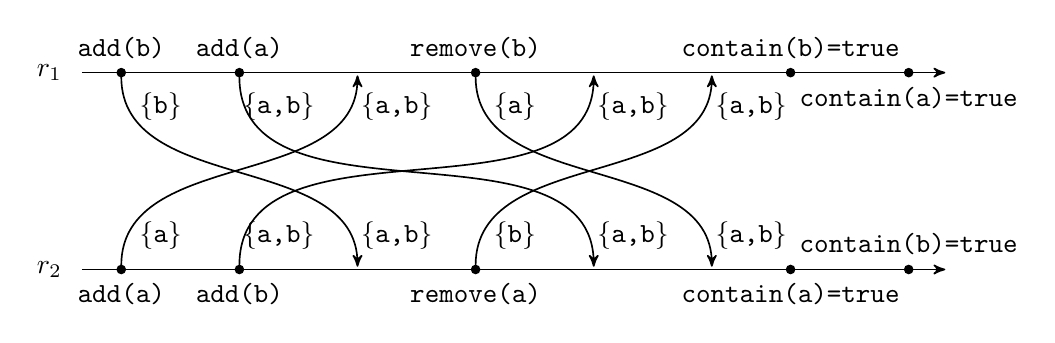
\begin{tikzpicture}[->,>=stealth',shorten >=1pt,auto,node distance=3cm,semithick, transform shape]

\draw (0, 0) -- (11, 0);
\draw (0, 2.5) -- (11, 2.5);

\node[label=left:{$r_2$}] at (0, 0) {};
\node[label=left:{$r_1$}] at (0, 2.5) {};

\node[draw,circle,fill=black,scale=0.3,label=below:{\texttt{add(a)}}](r21) at (.5, 0) {};
\node[draw,circle,fill=black,scale=0.3,label=below:{\texttt{add(b)}}](r22) at (2, 0) {};
\node[draw,circle,fill=black,scale=0.3,label=below:{\texttt{remove(a)}}](r23) at (5, 0) {};
\node[draw,circle,fill=black,scale=0.3,label=below:{\texttt{contain(a)=true}}] at (9, 0) {};
\node[draw,circle,fill=black,scale=0.3,label=above:{\texttt{contain(b)=true}}] at (10.5, 0) {};

\node[draw,circle,fill=black,scale=0.3,label=above:{\texttt{add(b)}}](r11) at (.5, 2.5) {};
\node[draw,circle,fill=black,scale=0.3,label=above:{\texttt{add(a)}}](r12) at (2, 2.5) {};
\node[draw,circle,fill=black,scale=0.3,label=above:{\texttt{remove(b)}}](r13) at (5, 2.5) {};
\node[draw,circle,fill=black,scale=0.3,label=above:{\texttt{contain(b)=true}}] at (9, 2.5) {};
\node[draw,circle,fill=black,scale=0.3,label=below:{\texttt{contain(a)=true}}] at (10.5, 2.5) {};

\node[label=above:{\texttt{\{a\}}}] at (1, 0) {};
\node[label=above:{\texttt{\{a,b\}}}] at (2.5, 0) {};
\node[label=above:{\texttt{\{a,b\}}}] at (4, 0) {};
\node[label=above:{\texttt{\{b\}}}] at (5.5, 0) {};
\node[label=above:{\texttt{\{a,b\}}}] at (7, 0) {};
\node[label=above:{\texttt{\{a,b\}}}] at (8.5, 0) {};

\node[label=below:{\texttt{\{b\}}}] at (1, 2.5) {};
\node[label=below:{\texttt{\{a,b\}}}] at (2.5, 2.5) {};
\node[label=below:{\texttt{\{a,b\}}}] at (4, 2.5) {};
\node[label=below:{\texttt{\{a\}}}] at (5.5, 2.5) {};
\node[label=below:{\texttt{\{a,b\}}}] at (7, 2.5) {};
\node[label=below:{\texttt{\{a,b\}}}] at (8.5, 2.5) {};

\draw (r11) edge[out=-90,in=90] (3.5, 0);
\draw (r12) edge[out=-90,in=90] (6.5, 0);
\draw (r13) edge[out=-90,in=90] (8, 0);

\draw (r21) edge[out=90,in=-90] (3.5, 2.5);
\draw (r22) edge[out=90,in=-90] (6.5, 2.5);
\draw (r23) edge[out=90,in=-90] (8, 2.5);

\end{tikzpicture}  
% }
\caption{A non-linearizable OR-Set execution. Edges represent propagation of updates. Each replica is annotated with labels showing the evolution of the set object after each update.}
\label{fig:crdt:intro}
\end{figure}

%\emph{Conflict-free replicated data types} (CRDTs)~\cite{DBLP:conf/sss/ShapiroPBZ11} efficiently resolve the effects of concurrent updates to replicated data. In 
For instance, Figure~\ref{fig:crdt:intro} pictures an execution of a CRDT called \emph{OR-Set}~\cite{DBLP:conf/sss/ShapiroPBZ11}, a set data type with standard \texttt{add(\_)}, \texttt{remove(\_)}, \texttt{contains(\_)} operations. \texttt{add(\_)} and \texttt{remove(\_)} are the only update operations. Two updates are in conflict if they are trying to insert or remove the same element, and possible conflicts are resolved by assuming that an \texttt{add(\_)} operation will always ``win'' among multiple conflicting concurrent updates, i.e., it will overwrite their effect. In Figure~\ref{fig:crdt:intro}, each replica executes the first two \texttt{add} operations in isolation (without being aware of operations on the other replica), receives the first \texttt{add} update from the other replica, and executes a \texttt{remove} operation before receiving the second \texttt{add} update from the other replica (as mentioned above, updates are propagated to other replicas asynchronously). The element $b$, resp., $a$, is again a member of the set on the top replica, resp., bottom replica, after receiving the last \texttt{add} update because the latter is concurrent (not causally related) to the \texttt{remove} on the receiving replica and the conflict is resolved by assuming that the \texttt{add} wins. This is witnessed by the last two \texttt{contains} operations on each replica that both return \texttt{true}. Note that this execution is an instance of \emph{weak consistency} since the return values of the \texttt{contains} operations cannot be explained using an interleaving of these operations (consistent with the order between operations on the same replica) as in classic variations of strong consistency, e.g., sequential consistency~\cite{DBLP:journals/tc/Lamport79} or linearizability\cite{DBLP:journals/toplas/HerlihyW90}.
%In figure \ref{fig:crdt:intro}, \texttt{read()} can seen as performing \texttt{contain(\_)} on $a$ and $b$. 

%In each replica $r_i$, everything seems fine when only \texttt{add(\_)} is happening. In $r_1$, after adding $a$ and $b$ and getting the update from $r_2$, the internal set contains both $a$ and $b$. After performing \texttt{remove(b)}, $b$ gets remove from the set. Now, the update of \texttt{add(b)} from $r_2$ reaches $r_1$. Since last \texttt{remove(b)} on $r_1$ and \texttt{add(b)} from $r_2$ are concurrent, meaning they are not causally related, they are in conflict. The OR-Set resolves them to the \texttt{add(b)}, so $b$ gets added in the set. Then the \texttt{remove(a)} from $r_2$ reaches to $r_1$. Like before, the \texttt{add(a)} on $r_1$ and \texttt{remove(a)} from $r_2$ are in conflict. The OR-Set resolves them to the \texttt{add(a)} and ignores the \texttt{remove(b)} from $r_2$. So $a$ and $b$ both persists in the set. The same can be explained for $r_2$'s observation. It can be shown, this behavior is not linearizable. This behavior is not possible when strong guarantees are promised.
%Similarly, \emph{And-Set} is a CRDT in which \texttt{remove(\_)} always wins among multiple conflicting updates.

%Recent distributed systems have introduced variations of familiar abstract data types (ADTs) like counters, registers, flags, and sets, that provide high availability and partition tolerance. These \emph{conflict-free replicated data types} (CRDTs)~\cite{DBLP:conf/sss/ShapiroPBZ11} efficiently resolve the effects of concurrent updates to replicated data. Naturally, they weaken consistency guarantees to achieve availability and partition-tolerance, and various notions of \emph{weak consistency} capture such guarantees~\cite{DBLP:conf/pdis/TerryDPSTW94, DBLP:conf/sosp/TerryTPDSH95, DBLP:conf/popl/MansonPA05, DBLP:journals/ftpl/Burckhardt14, DBLP:conf/popl/BurckhardtGYZ14}.

\begin{figure}[t]
  \centering
  \setlength{\tabcolsep}{1em}
\renewcommand{\arraystretch}{1.2}
\begin{tabular}{lr}
  \toprule
  Data Types & Complexity \\
  \cmidrule(lr){1-2}
  Add-Wins Set, Remove-Wins Set         & {\sc np}-complete \\
  Enable-Wins Flag, Disable-Wins Flag   & {\sc np}-complete \\
  Sets \& Flags — with bounded domains  & {\sc ptime} \\
  Last-Writer-Wins Register ({\sc lww}) & {\sc np}-complete \\
  Multi-Value Register ({\sc mvr})      & {\sc np}-complete \\
  Registers – with unique values        & {\sc ptime} \\
  Replicated Counters                   & {\sc np}-complete \\
  Counters – with bounded replicas      & {\sc ptime} \\
  Replicated Growable Array ({\sc rga}) & {\sc ptime} \\
  \bottomrule
\end{tabular}

  \caption{The complexity of consistency checking for various replicated data types. 
  %We demonstrate intractability and tractability results in Sections~\ref{sec:intractability} and~\ref{sec:algorithms}, respectively.
  }
  \label{fig:results}
\end{figure}

In this thesis we study the tractability of checking whether an execution of a CRDT conforms to the intended specification for different classes of data types; Figure~\ref{fig:results} summarizes some of our results. This problem is particularly relevant as distributed-system testing tools like Jepsen~\cite{MISC:Jepsen} are appearing; without efficient, general consistency-checking algorithms, such tools could be limited to specialized classes of errors like node crashes. 

Our study proceeds in two parts. First, to precisely characterize the consistency of various CRDTs, and facilitate symbolic reasoning, we develop novel logical characterizations to capture their guarantees. These characterizations integrate the data type semantics into the consistency guarantees, as opposed to existing formalizations, e.g.,~\cite{DBLP:journals/ftpl/Burckhardt14, DBLP:conf/popl/BurckhardtGYZ14}, of eventual consistency~\cite{DBLP:conf/sosp/TerryTPDSH95}, causal consistency~\cite{DBLP:journals/cacm/Lamport78}, sequential consistency, or linearizability, where the data type semantics is a parameter of the consistency specification. 

Second, we demonstrate the intractability of several CRDTs by reduction from propositional satisfiability (SAT) problems, and we develop tractable consistency-checking algorithms for individual data types and special cases. Previous work has mostly focused on the problem of checking conformance to \emph{strong} notions of consistency, e.g., checking for sequential consistency~\cite{DBLP:conf/cav/HenzingerQR99a, DBLP:journals/tpds/Qadeer03, DBLP:conf/cav/BinghamCHQZ04, DBLP:conf/pldi/BurckhardtAM07}, serializability~\cite{DBLP:conf/fmcad/0002OPTZ07, DBLP:conf/cav/FarzanM08, DBLP:conf/pldi/GuerraouiHJS08, DBLP:conf/pldi/EmmiMM10}, or linearizability~\cite{DBLP:journals/jpdc/WingG93, DBLP:conf/pldi/BurckhardtDMT10, DBLP:conf/pldi/EmmiEH15, DBLP:journals/concurrency/Lowe17}. 


%\subsection{State of the Art}
%
%The consistency models to specify these replicated data types.
%Many have considered consistency models applicable to CRDTs, including causal consistency~\cite{DBLP:journals/cacm/Lamport78}, sequential consistency~\cite{DBLP:journals/tc/Lamport79}, linearizability~\cite{DBLP:journals/toplas/HerlihyW90}, session consistency~\cite{DBLP:conf/pdis/TerryDPSTW94}, eventual consistency~\cite{DBLP:conf/sosp/TerryTPDSH95}, and happens-before consistency~\cite{DBLP:conf/popl/MansonPA05}. Burckhardt et al.~\cite{DBLP:journals/ftpl/Burckhardt14, DBLP:conf/popl/BurckhardtGYZ14} propose a unifying framework to formalize these models. Many have also studied the complexity of verifying data-type agnostic notions of consistency, including serializability, sequential consistency and linearizability~\cite{DBLP:journals/jacm/Papadimitriou79b, DBLP:journals/siamcomp/GibbonsK97, DBLP:journals/iandc/AlurMP00, DBLP:conf/spaa/BinghamCH03, DBLP:conf/cav/FarzanM08, DBLP:conf/esop/BouajjaniEEH13, DBLP:conf/netys/Hamza15}, as well as causal consistency~\cite{DBLP:conf/popl/BouajjaniEGH17}.
%% Our definition of the replicated LWW register corresponds to the notion of causal convergence in~\cite{DBLP:conf/popl/BouajjaniEGH17}. This work studies the complexity of the admissibility problem for the replicated LWW register. It shows that this problem is NP-complete in general and polynomial time when each value is written only once. 
%% Our NP-completeness result is stronger since it assumes a fixed number of replicas, and our algorithm for the case of unique values is more general and can be applied uniformly to MVR and RGA. 
%Bouajjani et al.~\cite{DBLP:journals/iandc/BouajjaniEEH18, DBLP:journals/pacmpl/EmmiE18} consider the complexity for individual linearizable collection types. Others have developed effective consistency checking algorithms for sequential consistency~\cite{DBLP:conf/cav/HenzingerQR99a, DBLP:journals/tpds/Qadeer03, DBLP:conf/cav/BinghamCHQZ04, DBLP:conf/pldi/BurckhardtAM07}, serializability~\cite{DBLP:conf/fmcad/0002OPTZ07, DBLP:conf/cav/FarzanM08, DBLP:conf/pldi/GuerraouiHJS08, DBLP:conf/pldi/EmmiMM10}, linearizability~\cite{DBLP:journals/jpdc/WingG93, DBLP:conf/pldi/BurckhardtDMT10, DBLP:conf/pldi/EmmiEH15, DBLP:journals/concurrency/Lowe17}, and even weaker notions like eventual consistency~\cite{DBLP:conf/popl/BouajjaniEH14} and sequential happens-before consistency~\cite{DBLP:conf/cav/EmmiE18, DBLP:journals/pacmpl/EmmiE19}.
%
%
%\subsection{Contribution}
%
%In this work we study the tractability of CRDT consistency checking. In particular, we consider \emph{runtime verification}: deciding whether a given execution of a CRDT is consistent with its ADT specification. This problem is particularly relevant as distributed-system testing tools like Jepsen~\cite{MISC:Jepsen} are appearing; without efficient, general consistency-checking algorithms, such tools could be limited to specialized classes of errors like node crashes.
%
%Our study proceeds in three parts.
%First, to precisely characterize the consistency of various CRDTs, and facilitate symbolic reasoning, we develop novel logical characterizations to capture their guarantees.
%Second, we demonstrate the intractability of several replicated data types by reduction from propositional satisfiability (SAT) problems.
%Third, we develop tractable consistency-checking algorithms for individual data types and special cases: replicated growing arrays; multi-value and last-writer-wins registers, when each value is written only once; counters, when replicas are bounded; and sets and flags, when their sizes are also bounded.





%%%%%%%%%%
% Transaction
%%%%%%%%%%

\section{Transactional Systems}\label{sec:intro:trans}


% \texttt{Payment(k)} \\
% \texttt{x = read_balance()} \\
% \texttt{x = read_balance()} \\ 
% \texttt{update_balance(x - k)} \\

\begin{figure}
    \centering
%    \begin{minipage}{.45\textwidth}
        \resizebox{.45\textwidth}{!}{
         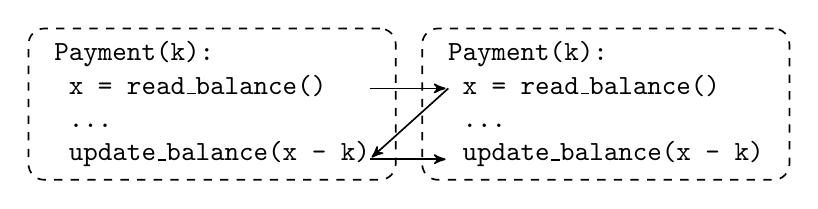
\begin{tikzpicture}[->,>=stealth',shorten >=1pt,auto,node distance=3cm,
           semithick, transform shape]
          \node[draw,dashed,rounded corners=2mm] (t1) at (0, 0) {\begin{tabular}{l}
            \texttt{Payment(k):} \\
            \texttt{  x = read\_balance()} \\
            \texttt{  ...} \\ 
            \texttt{  update\_balance(x - k)} \end{tabular}};
            \node[draw,dashed,rounded corners=2mm] (t2) at (5, 0) {\begin{tabular}{l}
              \texttt{Payment(k):} \\
              \texttt{  x = read\_balance()} \\
              \texttt{  ...} \\ 
              \texttt{  update\_balance(x - k)} \end{tabular}};
          \path (2, 0.2) edge (3, 0.2);
          \path (3, 0.2) edge (2, -0.7);
          \path (2, -0.7) edge (3, -0.7);
        %   \path (t1) edge[red, bend left] node {$\co$} (t2);
        %   \path (t4_2) edge node {$\po$} (t4_3);
        %   \path (t2) edge[blue, bend left] node {$\co$} (t1);
         \end{tikzpicture}  
        }
        \caption{A concurrent program. Edges show a non-transactional execution where both reads execute before a write.}
        \label{fig:txn:intro:1}
%       \end{minipage}
%       \hspace{.5cm}
%       \begin{minipage}{.45\textwidth}
%        \resizebox{\textwidth}{!}{
%         \begin{tikzpicture}[->,>=stealth',shorten >=1pt,auto,node distance=3cm,
%           semithick, transform shape]
%          \node[draw, rounded corners=2mm] (t1) at (0, 0) {\begin{tabular}{l}
%            \texttt{Payment(k):} \\
%            \texttt{  x = read\_balance()} \\
%            \texttt{  ...} \\ 
%            \texttt{  update\_balance(x - k)} \end{tabular}};
%            \node[draw, rounded corners=2mm] (t2) at (5, 0) {\begin{tabular}{l}
%              \texttt{Payment(k):} \\
%              \texttt{  x = read\_balance()} \\
%              \texttt{  ...} \\
%              \texttt{  update\_balance(x - k) } \\
%              \texttt{  // error -> rollback } \end{tabular}};
%        %   \path (t4_1) edge node {$\po$} (t4_2);
%        %   \path (t1) edge[red, bend left] node {$\co$} (t2);
%        %   \path (t4_2) edge node {$\po$} (t4_3);
%        %   \path (t2) edge[blue, bend left] node {$\co$} (t1);
%         \end{tikzpicture}  
%        }
%        \caption{Transactional execution}
%        \label{fig:txn:intro:2}
%    \end{minipage}
% \caption{Behaviors in non-transactional and transactional system}
\end{figure}

Transactions simplify concurrent programming by enabling multiple computations on shared data that are isolated from other concurrent computations and resilient to failures.
As an illustrating example, consider the \textsf{Payment} procedure in Figure \ref{fig:txn:intro:1} to be executed by two different processes. If we allow the internal read and write operations to be interleaved, we can have a scenario where both reads happen before a write. This would allow a user to pay €200 while his balance decreases only by €100. Executing the code of \textsf{Payment} as a transaction can disable such a behavior since each invocation is executed in isolation without interference from the other invocation. 
Modern databases provide transactions in various forms corresponding to different tradeoffs between consistency and availability. The strongest level of consistency is achieved with \emph{serializable} transactions~\cite{DBLP:journals/jacm/Papadimitriou79b} whose outcome in concurrent executions is the same as if the transactions were executed atomically in some order. Unfortunately, serializability carries a significant penalty on the availability of the system assuming, for instance, that the database is accessed over a network that can suffer from partitions or failures. For this reason, modern databases often provide weaker guarantees about transactions, formalized by weak consistency models, e.g., causal consistency~\cite{DBLP:journals/cacm/Lamport78} and snapshot isolation~\cite{DBLP:conf/sigmod/BerensonBGMOO95}.

Implementations of large-scale databases providing transactions are difficult to build and test. For instance, distributed (replicated) databases must account for partial failures, where some components or the network can fail and produce incomplete results. Ensuring fault-tolerance relies on intricate protocols that are difficult to design and reason about. The black-box testing framework Jepsen~\cite{jepsen} found a remarkably large number of subtle problems in many production distributed databases. %\footnote{https://www.infoq.com/presentations/partitioning-comparison}.

Testing a transactional database raises two issues: (1) deriving a suitable set of testing scenarios, e.g., faults to inject into the system and the set of transactions to be executed, and (2) deriving efficient algorithms for checking whether a given execution satisfies the considered consistency model. The Jepsen framework aims to address the first issue by using randomization, 
%shows that the first issue can be solved using randomization, 
e.g., introducing faults at random and choosing the operations in a transaction randomly. The effectiveness of this approach has been proved formally in recent work~\cite{DBLP:journals/pacmpl/OzkanMNBW18}. The second issue is, however, largely unexplored. Jepsen checks consistency in a rather ad-hoc way, focusing on specific classes of violations to a given consistency model, e.g., dirty reads (reading values from aborted transactions). This problem is challenging because the consistency specifications are non-trivial and they cannot be checked using, for instance, standard local assertions added to the client's code. 

Besides serializability, the complexity of checking correctness of an execution w.r.t. some consistency model is unknown. Checking serializability has been shown to be NP-complete~\cite{DBLP:journals/jacm/Papadimitriou79b}, and checking causal consistency in a \emph{non-transactional} context is known to be polynomial time~\cite{DBLP:conf/popl/BouajjaniEGH17}. In this thesis, we try to fill this gap by investigating the complexity of this problem w.r.t. several consistency models and, in the case of NP-completeness, devising algorithms that are polynomial time assuming fixed bounds for certain parameters of the input executions, e.g., the number of sessions. 

%
%The only result that explores the complexity of this problem 
%
%Except for  serializability, in which case it has been shown that checking  be NP-complete~\cite{DBLP:journals/jacm/Papadimitriou79b}
%% testing, i.e., randomly choosing the faults injected into the system and the transactions to be executed is enough to reveal a
%
%
%The success of Jepsen relies on random transactions as well as randomly introduced partition faults, therefore it is solved. We tackle the second issue for a series of consistency models (Jepsen implements a test of linearizability https://github.com/jepsen-io/knossos and an ad-hoc test for causal consistency restricted to bounded executions, \url{https://github.com/jepsen-io/jepsen/blob/f345226dba1266bc37487d734a02caddf7d1d125/jepsen/src/jepsen/tests/causal.clj})
We consider several consistency models that are the most prevalent in practice. The weakest of them, \emph{Read Committed} (RC)~\cite{DBLP:conf/sigmod/BerensonBGMOO95}, requires that every value read in a transaction is written by a committed transaction. \emph{Read Atomic} (RA)~\cite{DBLP:conf/concur/Cerone0G15} requires that successive reads of the same variable in a transaction return the same value (also known as Repeatable Reads~\cite{DBLP:conf/sigmod/BerensonBGMOO95}), and that a transaction ``sees'' the values written by previous transactions in the same session. In general, we assume that transactions are organized in \emph{sessions}~\cite{DBLP:conf/pdis/TerryDPSTW94}, an abstraction of the sequence of transactions performed during the execution of an application.
\emph{Causal Consistency} (CC)~\cite{DBLP:journals/cacm/Lamport78} requires that if a transaction~$\tr_1$ ``affects'' another transaction $\tr_2$, e.g., $\tr_1$ is ordered before $\tr_2$ in the same session or $\tr_2$ reads a value written by $\tr_1$, then these two transactions are observed by any other transaction in this order. \emph{Prefix Consistency} (PC)~\cite{DBLP:conf/ecoop/BurckhardtLPF15} requires that there exists a total commit order between all the transactions such that each transaction observes a prefix of this sequence. \emph{Snapshot Isolation} (SI)~\cite{DBLP:conf/sigmod/BerensonBGMOO95} further requires that two different transactions observe different prefixes if they both write to a common variable.
%Two different transactions $\tr_1$ and $\tr_2$ may observe the same prefix, which is not allowed under \emph{Snapshot Isolation} (SI)~\cite{DBLP:conf/sigmod/BerensonBGMOO95} when these two transactions write on a common variable. 
%Finally, we also provide new results concerning the problem of checking serializability (SER) that complement the known result about its NP-completeness. 

%The algorithmic issues we explore in this paper have led to a new specification framework for these consistency models that relies on the fact that the \emph{write-read} relation in an execution (also known as \emph{read-from}), relating reads with the transactions that wrote their value, can be defined effectively. The write-read relation can be extracted easily from executions where each value is written at most once (a variable can be written an arbitrary number of times). This can be easily enforced by tagging values with unique identifiers (e.g., a local counter that is incremented with every new write coupled with a client/session identifier)\footnote{This is also used in Jepsen, e.g., checking dirty reads in Galera~\cite{jepsen-galera}.}. Since practical database implementations are data-independent~\cite{DBLP:conf/popl/Wolper86}, i.e., their behavior doesn't depend on the concrete values read or written in the transactions, any potential buggy behavior can be exposed in executions where each value is written at most once. Therefore, this assumption is without loss of generality.
%
%Previous work~\cite{DBLP:conf/popl/BouajjaniEGH17,DBLP:conf/popl/BurckhardtGYZ14,DBLP:conf/concur/Cerone0G15} has formalized such consistency models using two auxiliary relations: a \emph{visibility} relation defining for each transaction the set of transactions it observes, and a \emph{commit order} defining the order in which transactions are committed to the ``global'' memory. An execution satisfying some consistency model is defined as the existence of a visibility relation and a commit order obeying certain axioms. In our case, the write-read relation derived from the execution plays the role of the visibility relation. This simplification allows us to state a series of axioms defining these consistency models, which have a common shape. Intuitively, they define lower bounds on the set of transactions $\tr_1$ that \emph{must} precede in commit order a transaction $\tr_2$ that is read in the execution. Besides shedding a new light on the differences between these consistency models, these axioms are essential for the algorithmic issues we investigate afterwards.

%Based on our formalization of these criteria, 
We establish that checking whether an execution satisfies RC, RA, or CC is polynomial time, while the same problem is NP-complete for PC and SI. Moreover, in the case of the NP-complete consistency models (PC, SI, SER), we show that their verification problem becomes polynomial time provided that, roughly speaking, the number of sessions in the input executions is considered to be fixed (i.e., not counted for in the input size). In more detail, we establish that checking SER reduces to a search problem in a space that has polynomial size when the number of sessions is fixed. (This algorithm applies to arbitrary executions, but its complexity would be exponential in the number of sessions in general.) Then, we show that checking PC or SI can be reduced in polynomial time to checking SER using a transformation of executions that, roughly speaking, splits each transaction in two parts: one part containing all the reads, and one part containing all the writes (SI further requires adding some additional variables in order to deal with transactions writing on a common variable).
We extend these results even further by relying on an abstraction of executions called \emph{communication graphs}~\cite{DBLP:journals/pacmpl/ChalupaCPSV18}. Roughly speaking, the vertices of a communication graph correspond to sessions, and the edges represent the fact that two sessions access (read or write) the same variable. We show that all these criteria are polynomial-time checkable provided that the \emph{biconnected} components of the communication graph are of fixed size. 

These results rely on a novel specification framework for such criteria which is of independent interest. 
This framework uses logical constraints, called \emph{axioms}, to characterize the
set of executions that conform to a particular consistency level. An execution is modeled using a specific set of
relations between events/transactions that describe control-flow
or data-flow dependencies: a program order $\po$ between events in the same
transaction, a session order $\so$ between transactions in the same session, 
and a write-read $\wro$ (read-from) relation that
associates each read event with a transaction that writes the value returned by
the read. These relations along with the events (also called, operations) in an
execution are called a \emph{history}. 
%The initial value of the key is supposed to be written in a fictitious transaction. 
A given history is said to satisfy a consistency model if it admits a \emph{total commit order} between its transactions
satisfying a specific set of axioms, which intuitively, 
define lower bounds on the set of transactions $\tr_1$ that \emph{must} precede in commit 
order a transaction $\tr_2$ that is read in the execution. 

We provide an experimental evaluation of our algorithms on executions of several production databases, that makes it possible to uncover new bugs or contradictions to their documentation. 
In particular, we show that, although the asymptotic complexity of our algorithms is exponential in general (w.r.t. the number of sessions), the worst-case behavior is not exercised in practice.

%=============
%
%Implementations of large-scale databases providing transactions are difficult to build and test. For instance, distributed (replicated) databases must account for partial failures, where some components or the network can fail and produce incomplete results. Ensuring fault-tolerance relies on intricate protocols that are difficult to design and reason about. The black-box testing framework Jepsen~\cite{jepsen} found a remarkably large number of subtle problems in many production distributed databases. \footnote{https://www.infoq.com/presentations/partitioning-comparison}.
%
%\subsection{State of the Art}
%
%Testing a transactional database raises two issues. First, deriving a suitable set of testing scenarios, e.g., faults to inject into the system and the set of transactions to be executed, and second, deriving efficient algorithms for checking whether a given execution satisfies the considered consistency model. The Jepsen framework aims to address the first issue by using randomization, 
%%shows that the first issue can be solved using randomization, 
%e.g., introducing faults at random and choosing the operations in a transaction randomly. The effectiveness of this approach has been proved formally in recent work~\cite{DBLP:journals/pacmpl/OzkanMNBW18}. The second issue is, however, largely unexplored. Jepsen checks consistency in a rather ad-hoc way, focusing on specific classes of violations to a given consistency model, e.g., dirty reads (reading values from aborted transactions). This problem is challenging because the consistency specifications are non-trivial and they cannot be checked using, for instance, standard local assertions added to the client's code. 
%
%Besides serializability, the complexity of checking correctness of an execution w.r.t. some consistency model is unknown. Checking serializability has been shown to be NP-complete~\cite{DBLP:journals/jacm/Papadimitriou79b}, and checking causal consistency in a \emph{non-transactional} context is known to be polynomial time~\cite{DBLP:conf/popl/BouajjaniEGH17}.
%
%\subsection{Contribution}
%
%In this work, we try to fill this gap by investigating the complexity of this problem w.r.t. several consistency models and, in the case of NP-completeness, devising algorithms that are polynomial time assuming fixed bounds for certain parameters of the input executions, e.g., the number of sessions. We consider several consistency models that are the most prevalent in practice. \emph{Read Committed} (RC)~\cite{DBLP:conf/sigmod/BerensonBGMOO95}, \emph{Read Atomic} (RA)~\cite{DBLP:conf/concur/Cerone0G15},  \emph{Causal Consistency} (CC)~\cite{DBLP:journals/cacm/Lamport78}, \emph{Prefix Consistency} (PC)~\cite{DBLP:conf/ecoop/BurckhardtLPF15}, \emph{Snapshot Isolation} (SI)~\cite{DBLP:conf/sigmod/BerensonBGMOO95} and Serializability (SER).

%
%The only result that explores the complexity of this problem 
%
%Except for  serializability, in which case it has been shown that checking  be NP-complete~\cite{DBLP:journals/jacm/Papadimitriou79b}
%% testing, i.e., randomly choosing the faults injected into the system and the transactions to be executed is enough to reveal a
%
%
%The success of Jepsen relies on random transactions as well as randomly introduced partition faults, therefore it is solved. We tackle the second issue for a series of consistency models (Jepsen implements a test of linearizability https://github.com/jepsen-io/knossos and an ad-hoc test for causal consistency restricted to bounded executions, \url{https://github.com/jepsen-io/jepsen/blob/f345226dba1266bc37487d734a02caddf7d1d125/jepsen/src/jepsen/tests/causal.clj})
% We consider several consistency models that are the most prevalent in practice. The weakest of them, \emph{Read Committed} (RC)~\cite{DBLP:conf/sigmod/BerensonBGMOO95}, requires that every value read in a transaction is written by a committed transaction. \emph{Read Atomic} (RA)~\cite{DBLP:conf/concur/Cerone0G15} requires that successive reads of the same variable in a transaction return the same value (also known as Repeatable Reads~\cite{DBLP:conf/sigmod/BerensonBGMOO95}), and that a transaction ``sees'' the values written by previous transactions in the same session. In general, we assume that transactions are organized in \emph{sessions}~\cite{DBLP:conf/pdis/TerryDPSTW94}, an abstraction of the sequence of transactions performed during the execution of an application.
% \emph{Causal Consistency} (CC)~\cite{DBLP:journals/cacm/Lamport78} requires that if a transaction~$\tr_1$ ``affects'' another transaction $\tr_2$, e.g., $\tr_1$ is ordered before $\tr_2$ in the same session or $\tr_2$ reads a value written by $\tr_1$, then these two transactions are observed by any other transaction in this order. \emph{Prefix Consistency} (PC)~\cite{DBLP:conf/ecoop/BurckhardtLPF15} requires that there exists a total commit order between all the transactions such that each transaction observes a prefix of this sequence. \emph{Snapshot Isolation} (SI)~\cite{DBLP:conf/sigmod/BerensonBGMOO95} further requires that two different transactions observe different prefixes if they both write to a common variable.
%Two different transactions $\tr_1$ and $\tr_2$ may observe the same prefix, which is not allowed under \emph{Snapshot Isolation} (SI)~\cite{DBLP:conf/sigmod/BerensonBGMOO95} when these two transactions write on a common variable. 
% Finally, we also provide new results concerning the problem of checking serializability (SER) that complement the known result about its NP-completeness. 

% The algorithmic issues we explore in this paper have led to a new specification framework for these consistency models that relies on the fact that the \emph{write-read} relation in an execution (also known as \emph{read-from}), relating reads with the transactions that wrote their value, can be defined effectively. The write-read relation can be extracted easily from executions where each value is written at most once (a variable can be written an arbitrary number of times). This can be easily enforced by tagging values with unique identifiers (e.g., a local counter that is incremented with every new write coupled with a client/session identifier)\footnote{This is also used in Jepsen, e.g., checking dirty reads in Galera~\cite{jepsen-galera}.}. Since practical database implementations are data-independent~\cite{DBLP:conf/popl/Wolper86}, i.e., their behavior doesn't depend on the concrete values read or written in the transactions, any potential buggy behavior can be exposed in executions where each value is written at most once. Therefore, this assumption is without loss of generality.

% Previous work~\cite{DBLP:conf/popl/BouajjaniEGH17,DBLP:conf/popl/BurckhardtGYZ14,DBLP:conf/concur/Cerone0G15} has formalized such consistency models using two auxiliary relations: a \emph{visibility} relation defining for each transaction the set of transactions it observes, and a \emph{commit order} defining the order in which transactions are committed to the ``global'' memory. An execution satisfying some consistency model is defined as the existence of a visibility relation and a commit order obeying certain axioms. In our case, the write-read relation derived from the execution plays the role of the visibility relation. This simplification allows us to state a series of axioms defining these consistency models, which have a common shape. Intuitively, they define lower bounds on the set of transactions $\tr_1$ that \emph{must} precede in commit order a transaction $\tr_2$ that is read in the execution. Besides shedding a new light on the differences between these consistency models, these axioms are essential for the algorithmic issues we investigate afterwards.

%%Based on our formalization of these criteria, 
%We establish that checking whether an execution satisfies RC, RA, or CC is polynomial time, while the same problem is NP-complete for PC and SI. Moreover, in the case of the NP-complete consistency models (PC, SI, SER), we show that their verification problem becomes polynomial time provided that, roughly speaking, the number of sessions in the input executions is considered to be fixed (i.e., not counted for in the input size). In more detail, we establish that checking SER reduces to a search problem in a space that has polynomial size when the number of sessions is fixed. (This algorithm applies to arbitrary executions, but its complexity would be exponential in the number of sessions in general.) Then, we show that checking PC or SI can be reduced in polynomial time to checking SER using a transformation of executions that, roughly speaking, splits each transaction in two parts: one part containing all the reads, and one part containing all the writes (SI further requires adding some additional variables in order to deal with transactions writing on a common variable).
%
%% We extend these results even further by relying on an abstraction of executions called \emph{communication graphs}~\cite{DBLP:journals/pacmpl/ChalupaCPSV18}. Roughly speaking, the vertices of a communication graph correspond to sessions, and the edges represent the fact that two sessions access (read or write) the same variable. We show that all these criteria are polynomial-time checkable provided that the \emph{biconnected} components of the communication graph are of fixed size.
%
%We provide an experimental evaluation of our algorithms on executions of CockroachDB~\cite{cockroach}, which claims to implement serializability~\cite{cockroach-claim} acknowledging however the possibility of anomalies, Galera~\cite{galera}, whose documentation contains contradicting claims about whether it implements snapshot isolation~\cite{galera-claim,galera-notclaim}, and AntidoteDB~\cite{antidote}, which claims to implement causal consistency~\cite{antidote-claim}.
%%Galera~\cite{galera}, and AntidoteDB~\cite{antidote}, which claim to implement serializability~\cite{cockroach-claim}, snapshot isolation~\cite{galera-claim} and causal consistency~\cite{antidote-claim}, respectively (in the default configuration). 
%Our implementation reports violations of these criteria in all cases. 
%%In the case of CockroachDB, the documentation admits possible anomalies while in the case of Galera we confirm an open issue submitted on Github~\cite{galera-issue}. 
%The consistency violations we found for AntidoteDB are novel and have been confirmed by its developers. We show that our algorithms are efficient and scalable.
%%and they outperform an encoding to boolean satisfiability of the consistency models. 
%In particular, we show that, although the asymptotic complexity of our algorithms is exponential in general (w.r.t. the number of sessions), the worst-case behavior is not exercised in practice.
%
%
%%%%%%
% \tool{}
%%%%%%

\section{Applications Using Transactional Systems}
\label{sec:app:intro}

Data storage is no longer about writing data to a single
disk with a single point of access. Modern applications require not just data
reliability, but also high-throughput concurrent accesses. 
Applications concerning supply chains, banking, etc. use traditional relational databases
for storing and processing data, whereas applications such as social networking
software and e-commerce platforms 
use cloud-based storage systems (such as Azure CosmosDb \cite{cosmosdb}, Amazon DynamoDb
\cite{DBLP:conf/sosp/DeCandiaHJKLPSVV07}, Facebook TAO \cite{DBLP:conf/usenix/BronsonACCDDFGKLMPPSV13}, etc.). We use the term \textit{storage
system} to refer to any such database system/service.

Providing high-throughput processing, unfortunately, comes at an unavoidable cost of weakening 
the guarantees offered to users.
Concurrently-connected clients may end up observing different views of the same data. 
These ``anomalies'' can be prevented by using a strong \textit{isolation (consistency) level}  
such as \textit{serializability}, which essentially offers a single view of the
data. However, since serializability requires expensive synchronization and incurs a high performance cost, 
most storage systems use weaker consistency models, such as RC, CC, or SI. 
%{\it Causal Consistency}~\cite{DBLP:journals/cacm/Lamport78,DBLP:conf/sosp/LloydFKA11,antidote-white-paper},
%{\it Snapshot Isolation}~\cite{DBLP:conf/sigmod/BerensonBGMOO95}, {\it Read
%Committed}~\cite{DBLP:conf/sigmod/BerensonBGMOO95}, etc. for better performance.
In a recent survey of
database administrators \cite{DBLP:conf/sigmod/Pavlo17}, 86\% of the participants responded that
most or all of the transactions in their databases execute at read committed (RC) consistency models.

\begin{figure}
  \centering
	\begin{minipage}{4.2cm}
		\begin{lstlisting}[basicstyle=\ttfamily\footnotesize,escapeinside={(*}{*)},language=MyLang]
// Append item to cart
AddItem(item i, userId) {
  Begin()
  key = "cart:" + userId
  cart = read(key)
  cart.append(i)
  write(key, cart)
  Commit()
}
		\end{lstlisting}
	\end{minipage}
	\hspace{-5mm}
	\begin{minipage}{4.2cm}
		\begin{lstlisting}[xleftmargin=4mm,basicstyle=\ttfamily\footnotesize,escapeinside={(*}{*)},language=MyLang]
// Fetch cart and delete item
DeleteItem(item i, userId) {
  Begin()
  key = "cart:" + userId
  cart = read(key)
  cart.remove(i)
  write(key, cart)
  Commit()
}
		\end{lstlisting}
	\end{minipage}
	
\vspace{-6mm}	
  \resizebox{8.5cm}{!}{
   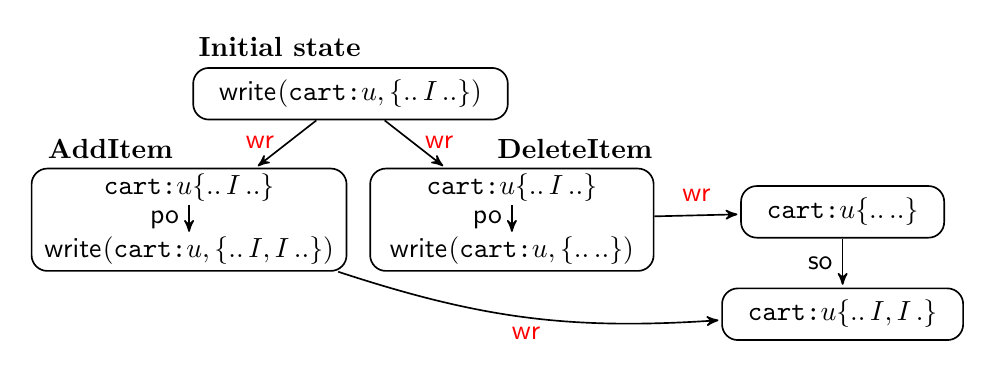
\begin{tikzpicture}[->,>=stealth',shorten >=1pt,auto,node distance=4cm,
     semithick, transform shape]
    \node (s11l) at (1.15, 2.1) {\textbf{Initial state}};
    \node[draw, rounded corners=2mm] (t0) at (2.05, 1.5) {\begin{tabular}{l} $\wrt{\texttt{cart:}u}{\{..\, I\, ..\}}$ \end{tabular}};
    \node[draw, rounded corners=2mm, minimum width=4cm, minimum height=1.3cm] (s1) at (0, -0.1) {};
    \node[style={inner sep=0,outer sep=0}] (s11) at (0, 0.3) {\begin{tabular}{l} $\rd{\texttt{cart:}u}{\{..\, I\, ..\}}$\end{tabular}};
    \node[style={inner sep=0,outer sep=0}] (s12) at (0, -0.5) {\begin{tabular}{l} $\wrt{\texttt{cart:}u}{\{..\, I,I\, ..\}}$ \end{tabular}};
    \node (s11l) at (-1, 0.8) {\textbf{AddItem}};
    \node[draw, rounded corners=2mm, minimum width=3.6cm, minimum height=1.3cm] (s2) at (4.1, -0.1) {};
    \node[style={inner sep=0,outer sep=0}] (s21) at (4.1, 0.3) {\begin{tabular}{l} $\rd{\texttt{cart:}u}{\{..\, I\, ..\}}$ \end{tabular}};
    \node[style={inner sep=0,outer sep=0}] (s22) at (4.1, -0.5) {\begin{tabular}{l} $\wrt{\texttt{cart:}u}{\{..\, ..\}}$ \end{tabular}};
    \node (s11l) at (4.9, 0.8) {\textbf{DeleteItem}};
    \node[draw, rounded corners=2mm] (r1) at (8.3, 0) {\begin{tabular}{l} $\rd{\texttt{cart:}u}{\{..\, ..\}}$ \end{tabular}};
    \node[draw, rounded corners=2mm] (r2) at (8.3, -1.3) {\begin{tabular}{l} $\rd{\texttt{cart:}u}{\{..\, I, I\, .\}}$ \end{tabular}};
    \path (s11) edge[left] node {$\po$} (s12);
    \path (s21) edge[left] node {$\po$} (s22);
    \path (t0) edge[left] node {$\wro$} (s1);
    \path (t0) edge[right] node {$\wro$} (s2);
    \path (r1) edge[left] node {$\so$} (r2);
    \path (s2) edge[above] node {$\wro$} (r1);
    \path (s1) edge[below,bend right=11] node {$\wro$} (r2);
%    \path (t0) edge[red, right, bend left=20] node[pos=0.4,xshift=-1] {$\wro$} (s11);
%    \path (t0) edge[red, left, bend right=20] node[pos=0.9,xshift=-1] {$\wro$} (s12);
   \end{tikzpicture}  
  }

%  \begin{lstlisting}[xleftmargin=4mm,basicstyle=\ttfamily\footnotesize,escapeinside={(*}{*)},language=MyLang,morekeywords={Test,GetCart}]
%Test: 
%{ AddItem(I, u); GetCart(u); GetCart(u) } || DeleteItem(I, u)
%		\end{lstlisting}
\vspace{-2mm}
	\caption{A simple shopping cart service.}
	\label{fig:motiv}
\vspace{-3mm}
\end{figure}

A weaker consistency model allows for more possible behaviors than stronger
consistency models. It is up to the developers then to ensure that their
application can tolerate this larger set of behaviors. Unfortunately, weak
consistency models are hard to understand or reason about
\cite{DBLP:conf/popl/BrutschyD0V17,adya-thesis} and resulting application bugs
can cause loss of business \cite{DBLP:conf/sigmod/WarszawskiB17}.
Consider a simple shopping cart application that stores a per-client shopping
cart in a key-value store (\textit{key} is the client ID and \textit{value} is a
multi-set of items). \figref{motiv} shows procedures for adding an item to the cart
(\texttt{AddItem}) and deleting \textit{all} instances of an item from the cart
(\texttt{DeleteItem}). Each procedure executes in a transaction, represented by
the calls to \texttt{Begin} and \texttt{Commit}. Suppose that initially, a user $u$ has 
a single instance of item $I$ in their cart.
Then the user connects to the application via two different
sessions (for instance, via two browser windows), adds $I$ in one session
(\texttt{AddItem($I$, $u$)}) and deletes $I$ in the other session
(\texttt{DeleteItem($I$, $u$)}). With serializability, the cart can either be
left in the state $\{ I \}$ (delete happened first, followed by the add) or $\emptyset$ (delete
happened second). However, with causal consistency (or read committed), it is possible that with two
sequential reads of the shopping cart, the cart is empty in the first read
(signaling that the delete has succeeded), but there are \textit{two} instances of $I$ 
in the second read! The history corresponding to this behavior 
is given on the bottom of Figure~\ref{fig:motiv} 
(read operations include the read value, and boxes group events from the same transaction).
Such anomalies, of deleted items reappearing, have been
noted in previous work \cite{DBLP:conf/sosp/DeCandiaHJKLPSVV07}. 


%\paragraph{Testing storage-based applications}
In this thesis, we address the problem of \textit{testing} code for correctness
against weak behaviors: a developer should be able to write a test that runs
their application and then asserts for correct behavior. 
The main difficulty today is getting coverage of weak behaviors during
the test. If one runs the test
against the actual production storage system, it is very likely to only result in
serializable behaviors because of their optimized implementation. For
instance, only 0.0004\% of all reads performed on Facebook's TAO storage system 
were not serializable \cite{DBLP:conf/sosp/LuVAHSTKL15}. 
Emulators, offered by cloud providers for local development, on the other hand, do not support weaker
consistency models at all \cite{cosmosdb-local}. Another option, possible when
the storage system is available open-source, is to set it up with a 
tool like Jepsen~\cite{jepsen} to inject noise (bring down replicas or
delay packets on the network). 
This approach is unable to provide good coverage at the level of client operations
\cite{DBLP:journals/pacmpl/RahmaniNDJ19} (\sectref{oltp}). Another line of work has focussed on finding
anomalies by identifying non-serializable behavior (\sectref{app:related}). Anomalies, however, do not
always correspond to bugs \cite{DBLP:conf/pldi/BrutschyD0V18,DBLP:journals/pvldb/GanRRB020}; they may
either not be important (e.g., gather statistics) or may already be handled in
the application (e.g., checking and deleting duplicate items).

We present MonkeyDB, a mock in-memory storage system meant for testing
correctness of storage-backed applications. 
MonkeyDB supports 
common APIs for accessing data (key-value updates, as well as SQL queries),
making it an easy substitute for an actual storage system. MonkeyDB
can be configured with one of several consistency models. 
%Currently,
%MonkeyDB supports Serializability, Causal Consistency as well as Read
%Committed. (Addition of other consistency models is easy.)
On a read operation, \tool{} computes the set of all possible return values
allowed under the chosen consistency models, and randomly returns one of them. The
developer can then simply execute their test multiple times to get coverage of
possible weak behaviors. For the program in \figref{motiv}, if we write a test
asserting that two sequential reads cannot return empty-cart followed by $\{I,
I\}$, then it takes only 20 runs of the test (on average) to fail the
assert. In contrast, the test does not fail when using MySQL with read committed, 
even after 100k runs. 
%MonkeyDB can work with any application with little to no modifications:
%a developer simply needs to link their tests to MonkeyDB, instead of the
%production storage system.

\paragraph{Design of \tool{}}
\tool{} does not rely on stress generation, fault
injection, or data replication. 
Rather, it works directly with a formalization of
the given consistency model in order to compute allowed return values. 

MonkeyDB implements a \emph{centralized} operational semantics for key-value stores, 
which is based on the axiomatic definitions of isolation (consistency)
levels that we introduced while investigating the algorithmic questions described in Section~\ref{sec:intro:trans}. 
Transactions are executed \emph{serially}, 
one after another, the concurrency being simulated during the handling of read events.  
This semantics maintains a history that contains all the past events (from all
transactions/sessions), and write events are simply added to the history. The
value returned by a read event is established based on a non-deterministic
choice of a write-read dependency (concerning this read event) that satisfies
the axioms of the considered consistency model.
%(MonkeyDB resolves any non-determinism in a random fashion). 
Depending on the weakness of the isolation
level, this makes it possible to return values written in arbitrarily ``old''
transactions, and simulate any concurrent behavior. For instance, the history in Figure~\ref{fig:motiv}
can be obtained by executing \texttt{AddItem}, \texttt{DeleteItem}, and then the two reads (serially).
The read in \texttt{DeleteItem} can take its value from the initial state and ``ignore'' the
previously executed \texttt{AddItem}, because the obtained history validates the axioms of 
causal consistency (or read committed). The same happens for the two later reads in the same
session, the first one being able to read from \texttt{DeleteItem} and the second one
from \texttt{AddItem}.

We formally prove that this semantics does indeed simulate any concurrent behavior, by 
showing that it is equivalent to a semantics where transactions are allowed to interleave.
In comparison with concrete implementations, this semantics makes it possible to handle 
a wide range of consistency models in a uniform way. It only has two sources of
non-determinism: 
the order in which entire transactions are submitted, and the choice of write-read dependencies in read 
events. This enable better coverage of possible behaviors, the penalty in performance not
being an issue in safety testing workloads which are usually small (see our evaluation). 


We also extend our semantics to cover SQL queries as well, by compiling SQL queries down to transactions with multiple key-value reads/writes. A table in a relational database is represented using a set of primary key values (identifying uniquely the set of rows) and a set of keys, one for each cell in the table. The set of primary key values is represented using a set of Boolean key-value pairs that simulate its characteristic function (adding or removing an element corresponds to updating one of these keys to $\btrue$ or $\bfalse$). Then, SQL queries are compiled to read or write accesses to the keys representing a table. For instance, a $\mathtt{SELECT}$ query that retrieves the set of rows in a table that satisfy a $\mathtt{WHERE}$ condition is compiled to (1) reading Boolean keys to identify the primary key values of the rows contained in the table, (2) reading keys that represent columns used in the $\mathtt{WHERE}$ condition, and (3) reading all the keys that represent cells in a row satisfying the $\mathtt{WHERE}$ condition. This rewriting contains the minimal set of accesses to the cells of a table that are needed to ensure the conventional specification of SQL.
It makes it possible to ``export'' formalizations of key-value store consistency models to SQL transactions.

We present an evaluation of MonkeyDB on several applications, showcasing its superior coverage of weak behaviors as well as bug-finding abilities.

%Modern applications require not just data
%reliability, but also high-throughput concurrent accesses. 
%Applications concerning supply chains, banking, etc. use traditional relational databases
%for storing and processing data, whereas applications such as social networking
%software and e-commerce platforms 
%use cloud-based storage systems (such as Azure CosmosDb \cite{cosmosdb}, Amazon DynamoDb
%\cite{DBLP:conf/sosp/DeCandiaHJKLPSVV07}, Facebook TAO \cite{DBLP:conf/usenix/BronsonACCDDFGKLMPPSV13}, etc.).
%
%
%%As applications have moved from a single-box environment to the cloud, the notion of
%%data persistence has also changed. It is no longer about storing data on a
%%single disk with a single point of access. Rather, modern applications such as
%%social networking software, e-commerce platforms, cloud micro-services, etc. are built using 
%%high-scale storage systems, such as Azure CosmosDb \cite{cosmosdb}, Amazon DynamoDb \cite{DBLP:conf/sigmod/Sivasubramanian12}, 
%%Facebook TAO \cite{DBLP:conf/usenix/BronsonACCDDFGKLMPPSV13}. Applications such as 
% 
%%These storage systems, commonly offered by most major cloud providers (such as
%%Azure CosmosDb \cite{cosmosdb}, Amazon DynamoDb \cite{DBLP:conf/sigmod/Sivasubramanian12}, 
%%Facebook TAO \cite{DBLP:conf/usenix/BronsonACCDDFGKLMPPSV13}, etc.)
%%create and manage multiple replicas of data. Having multiple replicas offers reliability and prevents
%%data loss, but it also offers availability and low-latency accesses by allowing
%%different clients to connect with different replicas. 
%
%Providing high-throughput processing, unfortunately, comes at an unavoidable cost of weakening 
%the guarantees offered to users.
%Concurrently-connected clients may end up observing different views of the same data. 
%These ``anomalies'' can be prevented by using a strong \textit{isolation level} 
%such as \textit{serializability}, which essentially offers a single view of the
%data. However, serializability requires expensive synchronization and incurs a high performance cost. As a
%consequence, most storage systems use weaker isolation levels, such as 
%{\it Causal Consistency}~\cite{DBLP:journals/cacm/Lamport78,DBLP:conf/sosp/LloydFKA11,antidote-white-paper},
%{\it Snapshot Isolation}~\cite{DBLP:conf/sigmod/BerensonBGMOO95}, {\it Read
%Committed}~\cite{DBLP:conf/sigmod/BerensonBGMOO95}, etc. for better performance.
%In a recent survey of
%database administrators \cite{DBLP:conf/sigmod/Pavlo17}, 86\% of the participants responded that
%most or all of the transactions in their databases execute at read committed isolation level.
%
%A weaker isolation level allows for more possible behaviors than stronger
%isolation levels. It is up to the developers then to ensure that their
%application can tolerate this larger set of behaviors. Unfortunately, weak
%isolation levels are hard to understand or reason about
%\cite{DBLP:conf/popl/BrutschyD0V17,adya-thesis} and resulting application bugs
%can cause loss of business \cite{DBLP:conf/sigmod/WarszawskiB17}.
%
%
%\subsection{State of the Art}
%
%This work addresses the problem of \textit{testing} code for correctness
%against weak behaviors: a developer should be able to write a test that runs
%their application and then asserts for correct behavior. 
%The main difficulty today is getting coverage of weak behaviors during
%the test. If one runs the test
%against the actual production storage system, it is very likely to only result in
%serializable behaviors because of their optimized implementation. For
%instance, only 0.0004\% of all reads performed on Facebook's TAO storage system 
%were not serializable \cite{DBLP:conf/sosp/LuVAHSTKL15}. 
%Emulators, offered by cloud providers for local development, on the other hand, do not support weaker
%isolation levels at all \cite{cosmosdb-local}. Another option, possible when
%the storage system is available open-source, is to set it up with a 
%tool like Jepsen~\cite{jepsen} to inject noise (bring down replicas or
%delay packets on the network). 
%This approach is unable to provide good coverage at the level of client operations
%\cite{DBLP:journals/pacmpl/RahmaniNDJ19} (\sectref{oltp}). Another line of work has focussed on finding
%anomalies by identifying non-serializable behavior (\sectref{app:related}). Anomalies, however, do not
%always correspond to bugs \cite{DBLP:conf/pldi/BrutschyD0V18,DBLP:journals/pvldb/GanRRB020}; they may
%either not be important (e.g., gather statistics) or may already be handled in
%the application (e.g., checking and deleting duplicate items).
%
%\subsection{Contribution}
%
%%Prior work on this problem has largely focussed on
%%formal verification techniques: to establish correctness of code against a specification 
%%of a particular isolation level \cite{DBLP:journals/pacmpl/RahmaniNDJ19,DBLP:journals/sigsoft/DabaghchianROMT17} (\akash{others?}). Verification requires
%%statically analyzing application code; with such an approach, in addition to
%%scalability problems, it is often difficult to support
%%various programming styles, libraries, frameworks and languages. 
%%For these reasons, testing is still the more widely adopted engineering practice. 
%%Our goal is support testing of any application, with little to no modifications.
%%We defer more details to the related work section.
%
%
%%
%%There 
%%is informal documentation available \cite{cosmosdb-consistency} as well as
%%formal specifications \akash{cite CosmosDb-TLA}, but none of it is immediately 
%%actionable for a developer. 
%
%
%%Modern applications such as social networking, ecommerce, etc., use
%%highly-available low-latency geo-replicated storage systems~\cite{cosmosdb} to
%%achieve high performance and scalability.
%%These storage systems must replicate data for persistence, and then allow
%%clients to connect with different replicas for availability on failures and for
%%low latency.
%%The replicas communicate updates to each other in the background using message
%%passing.
%%However, unfortunately, maintaining strong consistency across these replicas
%%requires global synchronization which incurs high performance overheads.
%%Moreover, as stated by the Consistency, Availability, and Partition-tolerance
%%(CAP) theorem~\cite{DBLP:journals/sigact/GilbertL02},
%%it is not possible for such storage systems to remain available and
%%simultaneously guarantee consistency under network partitions (which are
%%unavoidable).
%%Hence, to provide high availability and low latency, many distributed data
%%stores provide only weak consistency guarantees, formally defined as different
%%consistency models: {\it Causal Consistency}~\cite{DBLP:conf/popl/BouajjaniEGH17,DBLP:journals/cacm/Lamport78},
%%{\it Snapshot Isolation}~\cite{DBLP:conf/sigmod/BerensonBGMOO95}, and {\it Read
%%Committed}~\cite{DBLP:conf/sigmod/BerensonBGMOO95}, etc.
%%This current scenario is also showcased in a recent Database Admin
%%Survey~\cite{DBLP:conf/sigmod/Pavlo17} where more than 73\% participants responded that all the
%%transactions in their databases execute at read committed consistency level.
%
%%THE NEXT PARAGRAPH SHOULD BE ONLY ABOUT: PROGRAMMING ON TOP OF WEAK ISOLATION IS HARD. 
%
%%The weak isolation semantics of these consistency models permit various
%%anomalies that violate data consistency; for example, lost updates,
%%non-repeatable reads etc. 
%%(DIRTY READS IS NOT AN ANOMALY ABOVE READ COMMITTED).
%%Such anomalies often lead to undesirable executions in client applications and manifest in the form of invariant violations (assertion violations).
%%For example, consider an online store with a shopping cart
%%service~\ref{fig:motiv}.
%%If a user is accessing the cart from multiple clients, and deletes an item from
%%one client. 
%%Under weak consistency, not only that delete operation can take some time to be
%%visible through another client, but even after viewing deletion, the item could
%%appear again in the cart \cite{DBLP:conf/sosp/DeCandiaHJKLPSVV07}.
%%%\textcolor{blue}{Shopping cart example showing assertion violation on weak consistency.}
%%To prevent them, developers should be aware of such anomalies and use explicit
%%synchronization at appropriate program points in their applications. 
%%(TODO: LOCKING IS TOO SPECIFIC, USE SYNCHRONIZATION INSTEAD).
%%This requirement makes application development extremely challenging, because
%%such weak isolation semantics are hard to understand and
%%reason~\cite{DBLP:conf/popl/BrutschyD0V17,adya-thesis}, compared to the simple case of
%%serializability where one can argue about one transaction at a time. Further,
%%often these consistency levels are informally explained with low-level
%%implementation details, leading to poor understanding.
%%For example, Cosmos DB~\cite{cosmosdb} defines five levels of consistency with
%%only rough guidelines on which one to pick~\cite{cosmosdb-consistency}.
%%(THE FLOW IS A LITTLE BIT AKWARD: WEAK ISOLATION IS HARD TO UNDERSTAND COMPARED TO SERIALIZABILITY; MENTION THE Cosmos DB STUFF AS SUPPORT => INSERTING THE RIGHT SYNCHRONIZATION IS HARD => APPLICATION DEVELOPMENT IS HARD. WHY IS TESTING HARD BECAUSE WEAK ISOLATION IS COMPLICATED ?) 
%
%We present \tool{}, a mock in-memory storage system meant for testing
%correctness of storage-backed applications. 
%\tool{} supports 
%common APIs for accessing data (key-value updates, as well as SQL queries),
%making it an easy substitute for an actual storage system. \tool{}
%can be configured with one of several isolation levels. 
%%Currently,
%%\tool{} supports Serializability, Causal Consistency as well as Read
%%Committed. (Addition of other isolation levels is easy.)
%% On a read operation, \tool{} computes the set of all possible return values
%% allowed under the chosen isolation level, and randomly returns one of them. The
%% developer can then simply execute their test multiple times to get coverage of
%% possible weak behaviors. For the program in \figref{motiv}, if we write a test
%% asserting that two sequential reads cannot return empty-cart followed by $\{I,
%% I\}$, then it takes only 20 runs of the test (on average) to fail the
%% assert. In contrast, the test does not fail when using MySQL with read committed, 
%% even after 100k runs. 
%%\tool{} can work with any application with little to no modifications:
%%a developer simply needs to link their tests to \tool{}, instead of the
%%production storage system.
%
%\tool{} does not rely on stress generation, fault
%injection, or data replication. 
%Rather, it works directly with a formalization of
%the given isolation level in order to compute allowed return values.
%The theory behind \tool{} builds on the axiomatic definitions of isolation
%levels introduced in chapter \ref{chap:txn} \cite{DBLP:journals/pacmpl/BiswasE19}. These
%definitions use logical constraints (called \emph{axioms}) to characterize the
%set of executions of a key-value store that conform to a particular isolation
%level (we discuss SQL queries later).
%% These constraints refer to a specific set of
%% relations between events/transactions in an execution that describe control-flow
%% or data-flow dependencies: a program order $\po$ between events in the same
%% transaction, a session order $\so$ between transactions in the same session\footnote{A
%% session is a sequential interface to the storage system. It corresponds to what
%% is also called a connection.}, and a write-read $\wro$ (read-from) relation that
%% associates each read event with a transaction that writes the value returned by
%% the read. These relations along with the events (also called, operations) in an
%% execution are called a \emph{history}. The history corresponding to the 
%% shopping cart anomaly explained above is given on the bottom of Figure~\ref{fig:motiv}.
%% Read operations include the read value, and boxes group events from the same transaction.
%% %The initial value of the key is supposed to be written in a fictitious transaction. 
%% A history describes only the
%% interaction with the key-value store, omitting application side events (e.g., computing
%% the value to be written to a key). 
%
%% \tool{} implements a \emph{centralized} operational semantics for key-value stores, which is based on these axiomatic definitions. Transactions are executed \emph{serially}, one after another, the concurrency being simulated during the handling of read events.  
%% This semantics maintains a history that contains all the past events (from all
%% transactions/sessions), and write events are simply added to the history. The
%% value returned by a read event is established based on a non-deterministic
%% choice of a write-read dependency (concerning this read event) that satisfies
%% the axioms of the considered isolation level.
%% %(\tool{} resolves any non-determinism in a random fashion). 
%% Depending on the weakness of the isolation
%% level, this makes it possible to return values written in arbitrarily ``old''
%% transactions, and simulate any concurrent behavior. For instance, the history in Figure~\ref{fig:motiv}
%% can be obtained by executing \texttt{AddItem}, \texttt{DeleteItem}, and then the two reads (serially).
%% The read in \texttt{DeleteItem} can take its value from the initial state and ``ignore'' the
%% previously executed \texttt{AddItem}, because the obtained history validates the axioms of 
%% causal consistency (or read committed). The same happens for the two later reads in the same
%% session, the first one being able to read from \texttt{DeleteItem} and the second one
%% from \texttt{AddItem}.
%
%% We formally prove that this semantics does indeed simulate any concurrent behavior, by 
%% showing that it is equivalent to a semantics where transactions are allowed to interleave.
%% In comparison with concrete implementations, this semantics makes it possible to handle 
%% a wide range of isolation levels in a uniform way. It only has two sources of
%% non-determinism: 
%% the order in which entire transactions are submitted, and the choice of write-read dependencies in read 
%% events. This enable better coverage of possible behaviors, the penalty in performance not
%% being an issue in safety testing workloads which are usually small (see our evaluation). 
%
%We consider a set of micro-benchmarks Twitter \cite{twissandra}, Shopping Cart \cite{DBLP:conf/pldi/Sivaramakrishnan15}, Courseware \cite{DBLP:conf/esop/NairP020}, Treiber Stack \cite{DBLP:conf/cav/NagarMJ20} inspired from real-world applications 
%(\sectref{micro-benchmarks}) and evaluate the number of test iterations
%required to fail an invalid assertion 
%(\sectref{micro-assertion-violations}). We also measure the \textit{coverage} of
%weak behaviors provided by \tool{} (\sectref{micro-coverage}). Each of these
%applications were implemented based on their specifications described in prior
%work; they all use \tool{} as a library, via its KV interface.  
%
%
%We also extend our semantics to cover SQL queries as well, by compiling SQL queries down to transactions with multiple key-value reads/writes. Naturally, we considered OLTPBench \cite{DBLP:journals/pvldb/DifallahPCC13}, a popular benchmark suite of representative 
%OLTP workloads for relational databases. We picked a subset of OLTPBench, including TPC-C, for which we had reasonable assertions. We showed using our technique, \tool{} was able to violate these assertion under weak isolation levels.
%% A table in a relational database is represented using a set of primary key values (identifying uniquely the set of rows) and a set of keys, one for each cell in the table. The set of primary key values is represented using a set of Boolean key-value pairs that simulate its characteristic function (adding or removing an element corresponds to updating one of these keys to $\btrue$ or $\bfalse$). Then, SQL queries are compiled to read or write accesses to the keys representing a table. For instance, a $\mathtt{SELECT}$ query that retrieves the set of rows in a table that satisfy a $\mathtt{WHERE}$ condition is compiled to (1) reading Boolean keys to identify the primary key values of the rows contained in the table, (2) reading keys that represent columns used in the $\mathtt{WHERE}$ condition, and (3) reading all the keys that represent cells in a row satisfying the $\mathtt{WHERE}$ condition. This rewriting contains the minimal set of accesses to the cells of a table that are needed to ensure the conventional specification of SQL.
%% It makes it possible to ``export'' formalizations of key-value store isolation levels to SQL transactions.
%
%%This paper first presents an axiomatic semantics for various isolation levels 
%%in Key-Value stores that allows one to reason about the set of valid behaviors
%%under a given isolation level. We follow this by a non-deterministic operation
%%semantics, equivalent to the axiomatic semantics, where
%%each operation is cooperatively scheduled to execute one at a time (serially).
%%The operational semantics maintains a history of the read-write operations,
%%including a \textit{read-from} relationship that matches reads to previous
%%writes. On the submission of a new operation, this history is extended in
%%accordance with this operational semantics. \tool{} implements the operational
%%semantics, while resolving any non-determinism in a random fashion. 
%%We also extend our semantics to cover SQL queries as well, by compiling SQL
%%queries down to transactions with multiple key-value updates.
%
%% \paragraph{Contributions}
%%We implemented \tool{} to support an interface consistent with key-value
%%stores and databases, which allows us to directly run real applications unmodified. 
%%We evaluated \tool{} on a series of micro-benchmarks, inspired from real
%%applications, as well as the well-known OLTPBench \cite{DBLP:journals/pvldb/DifallahPCC13}
%%that is used for evaluating
%%databases on OLTP workloads. 
%
%% This paper makes the following contributions:
%% \begin{itemize}
%% \item We define an operational semantics for key-value stores under various
%%   isolation levels, which simulates all concurrent behaviors with executions
%%   where transactions execute serially (\sectref{op-kv}) and which is based 
%%   on the axiomatic definitions in~\cite{DBLP:journals/pacmpl/BiswasE19} (and outlined in \S\ref{sec:def}),
%% \item We broaden the scope of the key-value store semantics to SQL transactions
%%   using a compiler that rewrites SQL queries to key-value accesses (\sectref{SQL-to-KV}),
%% \item The operational semantics and the SQL compiler are implemented in a tool
%%   called \tool{} (\sectref{impl}). It randomly resolves possible choices to provide coverage
%%   of weak behaviors. It supports both a key-value interface as well as SQL,
%%   making it readily compatible with any storage-backed application.
%% \item We present an evaluation of \tool{} on several applications, showcasing
%% its superior coverage of weak behaviors as well as bug-finding abilities
%% (\sectref{micro}, \sectref{oltp}).\footnote{Source code of our benchmarks is available
%% as supplementary material.}
%% \end{itemize}

\section{Thesis Outline}

\emph{Weak consistency} concerning distributed datastores and applications remains the central topic of this dissertation. As discussed before, we studied the unexplored problems concerning \emph{weak consistency} from three domains - Conflict-Free Replicated Data Types, Transactional Systems and Applications implemented on top of transactional datastores. The remaining of this dissertation goes as following,

\begin{itemize}
  \item First in chapter \ref{chap:crdt}, we explore various Conflict-Free Replicated Data Types (CRDTs) and establish their formal characterizations. Then we study the asymptotic complexities of checking a given history for these CRDTs. Although the general problems (except Growing-Array) remains in NP-complete, we are able to give polynomial time algorithms for practical constraints, such as bounded number of replicas, using different values at each writes.
  \item Then in chapter \ref{chap:txn}, we explore the similar problems in the context of transactional systems. We study various levels of weak consistency for these systems and establish their formal characterizations. We study the asymptotic complexities of checking conformance of a given transactional history to a weak consistency criteria. We prove, for weaker consistency criteria, such as Causal Consistency, the complexities of this checking problem are polynomial time. But for stronger consistency models, such as Snapshot Isolation, they are NP-complete. But we provide polynomial time algorithm for the history whose the communication graphs have bounded size of biconnected components. We provide some performance analysis on some production databases doing comparisons against SAT solvers using SAT encodings of NP-complete problems.
  \item Next in chapter \ref{chap:dist-app} we look at the testing coverage problem of distributed applications built with transactional datastores. We implement \tool{} based on our previous work for transactional system. \tool{} transforms the high level database queries or calls to low level transactional key-value store operations. Then, using the characterizations for transactional systems for a given consistency model, it simulates possible cases probabilistically and give a better test coverages than current state of the art benchmark setups to find bugs within few attempts. We run tests on some popular benchmarks including OLTPBench to show it outperforms other existing tools.
\end{itemize}

At the end we conclude at chapter \ref{chap:conclusion} and discuss future works in section \ref{sec:global-future-work}.

  \chapter{Checking Consistency for Conflict-Free Replicated Data Types}
  \label{chap:crdt}

  %!TEX root = Thesis.tex

\section{Introduction}
\label{sec:crdt:intro}

Recent distributed systems have introduced variations of familiar abstract data types (ADTs) like counters, registers, flags, and sets, that provide high availability and partition tolerance. These \emph{conflict-free replicated data types} (CRDTs)~\cite{DBLP:conf/sss/ShapiroPBZ11} efficiently resolve the effects of concurrent updates to replicated data. Naturally, they weaken consistency guarantees to achieve availability and partition-tolerance, and various notions of \emph{weak consistency} capture such guarantees~\cite{DBLP:conf/pdis/TerryDPSTW94, DBLP:conf/sosp/TerryTPDSH95, DBLP:conf/popl/MansonPA05, DBLP:journals/ftpl/Burckhardt14, DBLP:conf/popl/BurckhardtGYZ14}.

In this work we study the tractability of CRDT consistency checking; Figure~\ref{fig:results} summarizes our results. In particular, we consider \emph{runtime verification}: deciding whether a given execution of a CRDT is consistent with its ADT specification. This problem is particularly relevant as distributed-system testing tools like Jepsen~\cite{MISC:Jepsen} are appearing; without efficient, general consistency-checking algorithms, such tools could be limited to specialized classes of errors like node crashes.

Our setting captures executions across a set of replicas as per-replica sequences of operations called \emph{histories}. Roughly speaking, a history is \emph{consistent} so long as each operation’s return value can be justified according to the operations that its replica has observed so far. In the setting of CRDTs, the determination of a replica’s observations is essentially an implementation choice: replicas are only obliged to observe their own operations, and the predecessors of those it has already observed. This relatively-weak constraint on replicas’ observations makes the CRDT consistency checking problem unique.

\begin{figure}[t]
  \centering
  \setlength{\tabcolsep}{1em}
\renewcommand{\arraystretch}{1.2}
\begin{tabular}{lr}
  \toprule
  Data Types & Complexity \\
  \cmidrule(lr){1-2}
  Add-Wins Set, Remove-Wins Set         & {\sc np}-complete \\
  Enable-Wins Flag, Disable-Wins Flag   & {\sc np}-complete \\
  Sets \& Flags — with bounded domains  & {\sc ptime} \\
  Last-Writer-Wins Register ({\sc lww}) & {\sc np}-complete \\
  Multi-Value Register ({\sc mvr})      & {\sc np}-complete \\
  Registers – with unique values        & {\sc ptime} \\
  Replicated Counters                   & {\sc np}-complete \\
  Counters – with bounded replicas      & {\sc ptime} \\
  Replicated Growable Array ({\sc rga}) & {\sc ptime} \\
  \bottomrule
\end{tabular}

  \caption{The complexity of consistency checking for various replicated data types. We demonstrate intractability and tractability results in Sections~\ref{sec:intractability} and~\ref{sec:algorithms}, respectively.}
  \label{fig:results}
\end{figure}

Our study proceeds in three parts. First, to precisely characterize the consistency of various CRDTs, and facilitate symbolic reasoning, we develop novel logical characterizations to capture their guarantees. Our logical models are built on a notion of \emph{abstract execution}, which relates the operations of a given history with three separate relations: a \emph{read-from} relation, governing the observations from which a given operation constitutes its own return value; a \emph{happens-before} relation, capturing the causal relationships among operations; and a \emph{linearization} relation, capturing any necessary arbitration among non-commutative effects which are executed concurrently, e.g.,~following a \emph{last-writer-wins} policy. Accordingly, we capture data type specifications with logical axioms interpreted over the read-from, happens-before, and linearization relations of abstract executions, reducing the consistency problem to: does there exist an abstract execution over the given history which satisfies the axioms of the given data type?

Second, we demonstrate the intractability of several replicated data types by reduction from propositional satisfiability (SAT) problems. In particular, we consider the 1-in-3 SAT problem~\cite{DBLP:books/fm/GareyJ79}, which asks for a truth assignment to the variables of a given set of clauses such that exactly one literal per clause is assigned true. Our reductions essentially simulate the existential choice of a truth assignment with the existential choice of the read-from and happens-before relations of an abstract execution. For a given 1-in-3 SAT instance, we construct a history of replicas obeying carefully-tailored synchronization protocols, which is consistent exactly when the corresponding SAT instance is positive.

Third, we develop tractable consistency-checking algorithms for individual data types and special cases: replicated growing arrays; multi-value and last-writer-wins registers, when each value is written only once; counters, when replicas are bounded; and sets and flags, when their sizes are also bounded. While the algorithms for each case are tailored to the algebraic properties of the data types they handle, they essentially all function by constructing abstract executions incrementally, processing replicas’ operations in prefix order.

The remainder of this article is organized around our three key contributions:
% \vspace{-3.5mm}
\begin{enumerate}

  \item We develop novel logical characterizations of consistency for the replicated register, flag, set, counter, and array data types (§\ref{sec:consistency});

  \item We develop novel reductions from propositional satisfiability problems to consistency checking to demonstrate intractability for replicated flags, sets, counters, and registers (§\ref{sec:intractability}); and

  \item We develop tractable consistency-checking algorithms for replicated growable arrays, registers, when written values are unique, counters, when replicas are bounded, and sets and flags, when their sizes are also bounded (§\ref{sec:algorithms}–\ref{sec:ptime:sets}).

\end{enumerate}
% \vspace{-1.5mm}
Section~\ref{sec:crdt:related} overviews related work, and Section~\ref{sec:conclusion} concludes.

  %!TEX root = ../../Thesis.tex

\section{A Logical Characterization of Replicated Data Types}
\label{sec:consistency}

In this section we describe an axiomatic framework for defining the semantics of replicated data types.
%To formalize the semantics of replicated data types we use several semantic domains defined hereafter.
We consider a set of method names $\methods$, and that
each method $\amethod \in \methods$ has a number of arguments and a return value sampled from
a data domain $\datadomain$. %We use a distinguished value $\bot$ to denote absence of return value.
%By an abuse of terminology, the methods that return a value different from $\bot$
%are called \emph{query methods} even though they may modify the state of the object.
%The set of query methods is denoted by $\queries$. TODO EXAMPLE.
We will use operation labels of the form
$\alabellongind{\argv}{\retv}{i}$ to represent the call of a
method $\amethod \in \methods$, with
argument $\argv \in \datadomain$, and resulting in the value $\retv \in
\datadomain$. Since there might be multiple calls to the same method with the same
arguments and result, labels are tagged with a unique identifier $i$. We will ignore identifiers when unambiguous.
%The set of all operation labels is denoted by $\labels$.
%The operation labels corresponding to query methods are called queries.
%For a given operation label $\ell=\alabellongind{\argv}{\retv}{i}$, ${\sf meth}

The interaction between a data type implementation and a client is represented by a \emph{history} $\hist=\tup{\Op, \RO}$ which consists of a set of operation labels $\Op$ and a partial \emph{replica order} $\RO$ ordering operations issued by the client on the same replica. Usually, $\RO$ is a union of sequences, each sequence representing the operations issued on the same replica, and the \emph{width} of $\RO$, i.e., the maximum number of mutually-unordered operations, gives the number of replicas in a given history.

To characterize the set of histories $\hist=\tup{\Op, \RO}$ admitted by a certain replicated data type, we use \emph{abstract executions} $\exec = \tup{ \rf,\hb,\lin }$, which include:
%a set of relations that concern
%%. The overarching principle is to say that a history is admitted if there exist several relations between the labels in the history which satisfy certain properties. These relations are concerned with
%the correctness of return values (the read-from relation), preserving causal dependencies between operations (the happens-before order), and modeling the conflict resolution policy (the linearization order). In this work, we consider replicated data types which satisfy \emph{causal consistency}~\cite{DBLP:journals/cacm/Lamport78}, i.e., updates which are related by cause and effect relations are observed by all replicas in the same order. %The properties of these different relations are expressed using a set of first-order axioms. 
%Therefore, an \emph{abstract execution} $\exec = \tup{ \rf,\hb,\lin }$ of the history $\hist=\tup{\Op, \RO}$  is:
\vspace{-2.5mm}
\begin{itemize}
  \item a \emph{read-from} binary relation $\rf$ over operations in $\Op$, which identifies the set of updates needed to ``explain'' a certain return value, e.g., a {\sf write} operation explaining the return value of a {\sf read},
  \item a strict partial \emph{happens-before} order $\hb$, which includes $\ro$ and $\rf$, representing the causality constraints in an execution, and
  \item a strict total \emph{linearization} order $\lin$, which includes $\hb$, used to model conflict resolution policies based on timestamps.
\end{itemize}
\vspace{-1mm}
In this work, we consider replicated data types which satisfy \emph{causal consistency}~\cite{DBLP:journals/cacm/Lamport78}, i.e., updates which are related by cause and effect relations are observed by all replicas in the same order. This follows from the fact that the happens-before order is constrained to be a partial order, and thus transitive (other forms of weak consistency don't pose this constraint). Some of the replicated data types we consider in this work do \emph{not} consider resolution policies based on timestamps and in those cases, the linearization order can be ignored.

A \emph{replicated data type} is defined by a set of first-order axioms $\Phi$ characterizing the relations in an abstract execution. 
A history $\hist$ is \emph{admitted} by a data type when there exists an abstract execution $\exec$ such that $\tup{\hist,\exec}\models\Phi$. The satisfaction relation $\models$ is defined as usual in first order logic. The \emph{admissibility problem} is the problem of checking whether a history $\hist$ is admitted by a given data type.

%More precisely, the axioms in $\Phi_{\rf}$ characterize a pair $\tup{\hist,\rf}$ formed of a history and a read-from relation, the axioms in $\Phi_{\hb}$ a triple $\tup{\hist,\rf,\hb}$ formed of a history, read-from relation, and happens-before order, and finally, $\Phi_{\lin}$ characterize abstract executions of histories $\tup{\hist,\rf,\hb,\lin}$. Their satisfaction relation $\models$ on such tuples is defined as usual.

%We say that a history $\hist$ is admitted by a data type $\Phi_{\rf}\cup \Phi_{\hb}\cup \Phi_{\lin}$ when there exists an abstract execution $\exec = \tup{ \rf,\hb,\lin }$ of $\hist$ such that $\tup{\hist,\rf}\models \Phi_{\rf}$, $\tup{\hist,\rf,\hb}\models \Phi_{\hb}$, and $\tup{\hist,\rf,\hb,\lin}\models \Phi_{\lin}$.



\begin{figure}[t]
  \footnotesize
  \hspace{-5mm}
  \begin{minipage}[t]{.48\linewidth}
    \begin{align*}
  & \text{\underline{{\sc ReadFrom}$(R)$}} \\
  & \forall o_1,o_2.\ \rf(o_1,o_2) \implies R(o_1,o_2)
  \\[1em]
  & \text{\underline{{\sc ReadFromMaximal}$(R)$}} \\
  & \forall o_1,o_2,o_3.\ \rf(o_1,o_2) \land R(o_3,o_2) \implies \\
  & \lnot\hb(o_1,o_3) \lor \lnot\hb(o_3,o_2)
  \\[1em]
  & \text{\underline{{\sc ReadAllMaximals}$(R)$}} \\
  & \forall o_1,o_2.\ \hb(o_1,o_2)\land R(o_1,o_2) \\
  & \implies \exists o_3.\ \hb^*(o_1,o_3)\land  \rf(o_3,o_2)
  \\[1em]
  & \text{\underline{{\sc ClosedRF}$(R)$}} \\
  & \forall o_1, o_2, o_3.\ R(o_1,o_2) \land \hb(o_1,o_3) \\
  & \land \rf(o_3,o_2) \implies \rf(o_1,o_2)
\end{align*}

  \end{minipage}
  \hfill
  \begin{minipage}[t]{.48\linewidth}
    \begin{align*}
  & \text{\underline{{\sc RetvalSet}$(X,v,Y)$}} \\
  & \forall o_1.\ {\sf meth}(o_1) = X\land {\sf ret}(o_1) = v \\
  & \Leftrightarrow \exists o_2.\ \rf(o_2,o_1) \land {\sf meth}(o_2) = Y \\
  & \quad \quad \quad \land {\sf arg}(o_1)={\sf arg}(o_2)
  \\[1em]
  & \text{\underline{\sc RetvalCounter}} \\
  & \forall o_1.\ {\sf meth}(o_1) = {\sf read} \\
  & \implies {\sf ret}(o_1) = |\{o_2: {\sf meth}(o_2) = {\sf inc}\land \rf(o_2,o_1)\}| \\
  & - |\{o_2: {\sf meth}(o_2) = {\sf dec}\land \rf(o_2,o_1)\}|
  \\[1em]
  & \text{\underline{\sc LinLWW}} \\
  & \forall o_1, o_2, o_3.\ \rf(o_1,o_2) \land {\sf meth}(o_3)={\sf write} \\
  & \land {\sf arg}_1(o_3)={\sf arg}(o_2)\land \hb(o_3,o_2) \implies \lin(o_3,o_1)
\end{align*}

  \end{minipage}
  \begin{align*}
  & \text{\underline{\sc RetvalReg}} \\
  & \forall o_1,v. {\sf meth}(o_1) = {\sf read} \land v\in {\sf ret}(o_1)
  \implies \exists! o_2. \rf(o_2,o_1) \land {\sf meth}(o_2) = {\sf write}
  \land {\sf arg}_2(o_2)=v
\end{align*}

  \vspace{-2em}
  \caption{The axiomatic semantics of replicated data types. Quantified variables are implicitly distinct, and $\exists! o$ denotes the existence of a unique operation $o$.}
  \label{fig:formulas:common}
  \vspace{-1em}
\end{figure}



In the following, we define the replicated data types with respect to which we study the complexity of the admissibility problem. The axioms used to define them are listed in Figure~\ref{fig:formulas:common} and Figure~\ref{fig:formulas:RGA}. These axioms use the function symbols {\sf meth}-od, {\sf arg}-ument, and {\sf ret}-urn interpreted over operation labels, whose semantics is self-explanatory. 
%Moreover, {\sf ReadOk} is a binary predicate interpreted over operation labels whose semantics is defined individually for each data type.

\subsection{Replicated Sets and Flags}

The Add-Wins Set and Remove-Wins Set~\cite{DBLP:journals/eatcs/ShapiroPBZ11}
are two implementations of a replicated set with operations {\sf add}($x$), {\sf remove}($x$), and {\sf contains}($x$) for adding, removing, and checking membership of an element $x$.
Although the meaning of these methods is self-evident from their names,
 the result of conflicting concurrent operations is not evident. When concurrent {\sf add}($x$) and {\sf remove}($x$)
 operations are delivered to a certain replica, the Add-Wins Set chooses to keep the element $x$ in the set, so every
 subsequent invocation of {\sf contains}($x$) on this replica returns $\mathit{true}$, while the Remove-Wins Set makes the dual choice
 of removing $x$ from the set.

The formal definition of their semantics uses abstract executions where the read-from relation associates sets of {\sf add}($x$) and {\sf remove}($x$)
operations to {\sf contains}($x$) operations. Therefore, the predicate ${\sf ReadOk}(o_1,o_2)$ is defined by
\begin{align*}
{\sf meth}(o_1) \in \{{\sf add},{\sf remove}\} \land {\sf meth}(o_2) ={\sf contains} \land {\sf arg}(o_1)= {\sf arg}(o_2)
\end{align*}
and the Add-Wins Set is defined by the following set of axioms:
\begin{align*}
&\textsc{ReadFrom}({\sf ReadOk}) \land \textsc{ReadFromMaximal}({\sf ReadOk})\ \land \\
& \textsc{ReadAllMaximals}({\sf ReadOk}) \land \textsc{RetvalSet}({\sf contains},\mathit{true},{\sf add})
\end{align*}
\textsc{ReadFromMaximal} says that every operation read by a {\sf contains}($x$) is maximal among its $\hb$-predecessors that add or remove $x$ while \textsc{ReadAllMaximals} says that all such maximal $\hb$-predecessors are read. The \textsc{RetvalSet} instantiation ensures that a {\sf contains}($x$) returns $\mathit{true}$ iff it reads-from at least one {\sf add}($x$).

The definition of the Remove-Wins Set is similar, except for the parameters of \textsc{RetvalSet}, which become
$
\textsc{RetvalSet}({\sf contains},\mathit{false},{\sf remove}),
$
i.e., a {\sf contains}($x$) returns $\mathit{false}$ iff it reads-from at least one {\sf remove}($x$).
%\end{example}

The Enable-Wins Flag and Disable-Wins Flag are implementations of a set of flags with operations: {\sf enable}($x$), {\sf disable}($x$), and {\sf read}($x$), where {\sf enable}($x$) turns the flag $x$ to true, {\sf disable}($x$) turns $x$ to false, while {\sf read}($x$) returns the state of the flag $x$. Their semantics is similar to the Add-Wins Set and Remove-Wins Set, respectively, where {\sf enable}($x$), {\sf disable}($x$), and {\sf read}($x$) play the role of {\sf add}($x$), {\sf remove}($x$), and {\sf contains}($x$), respectively. Their axioms are defined as above.

\subsection{Replicated Registers}

We consider two variations of replicated registers called Multi-Value Register (MVR) and Last-Writer-Wins Register (LWW)~\cite{DBLP:journals/eatcs/ShapiroPBZ11} which maintain a set of registers and provide {\sf write}($x$,$v$) operations for writing a value $v$ on a register $x$ and {\sf read}($x$) operations for reading the content of a register $x$ (the domain of values is kept unspecified since it is irrelevant). While a {\sf read}($x$) operation of MVR returns \emph{all} the values written by concurrent writes which are maximal among its happens-before predecessors, therefore, leaving the responsibility for solving conflicts between concurrent writes to the client, a {\sf read}($x$) operation of LWW returns a single value chosen using a conflict-resolution policy based on timestamps. Each written value is associated to a timestamp, and a {\sf read} operation returns the most recent value w.r.t. the timestamps. This order between timestamps is modeled using the linearization order of an abstract execution.

Therefore, the predicate ${\sf ReadOk}(o_1,o_2)$ is defined by
\begin{align*}
{\sf meth}(o_1) = {\sf write} \land {\sf meth}(o_2) ={\sf read} \land {\sf arg}_1(o_1)= {\sf arg}(o_2) \land {\sf arg}_2(o_1)\in {\sf ret}(o_2)
\end{align*}
(we use ${\sf arg}_1(o_1)$ to denote the first argument of a {\sf write} operation, i.e., the register name, and ${\sf arg}_2(o_1)$ to denote its second argument, i.e., the written value) and the MVR is defined by the following set of axioms:
\begin{align*}
&\textsc{ReadFrom}({\sf ReadOk})\land \textsc{ReadFromMaximal}({\sf ReadOk})\ \land \\
& \textsc{ReadAllMaximals}({\sf ReadOk})\land \textsc{RetvalReg}
\end{align*}
where \textsc{RetvalReg} ensures that a {\sf read}($x$) operation reads from a {\sf write}($x$,$v$) operation, for each value $v$ in the set of returned values~\footnote{For simplicity, we assume that every history contains a set of {\sf write} operations writing the initial values of variables, which precede every other operation in replica order.}.

LWW is obtained from the definition of MVR by replacing \textsc{ReadAllMaximals} with the axiom \textsc{LinLWW} which ensures that every {\sf write}($x$,\_) operation which happens-before a {\sf read}($x$) operation is linearized before the {\sf write}($x$,\_) operation from where the {\sf read}($x$) takes its value (when these two {\sf write} operations are different). This definition of LWW is inspired by the ``bad-pattern'' characterization in~\cite{DBLP:conf/popl/BouajjaniEGH17}, corresponding to their causal convergence criterion.

\subsection{Replicated Counters}\label{ssec:counter}

%TODO PROBABLY A GOOD IDEA TO MENTION SOME BASIC FACTS LIKE (A) WHAT YOU CALL A “COUNTER” IS IN FACT A COLLECTION OF COUNTERS, (B) WHAT ARE THE DOMAIN AND RANGE OF A COUNTER? E.G. DOMAIN IS PROBABLY SOME SET OF VARIABLE NAMES, AND RANGE IS PROBABLY INTEGERS… WITHOUT SAYING THIS, ONE MIGHT THINK THAT COUNTERS SHOULD ARE ALWAYS POSITIVE. ALSO: THIS KIND OF DISCUSSION SHOULD PROBABLY PRECLUDE EACH OF THESE SUBSECTIONS.

The replicated counter datatype~\cite{DBLP:journals/eatcs/ShapiroPBZ11} maintains a set of counters interpreted as integers (the counters can become negative). This datatype provides  operations {\sf inc}($x$) and {\sf dec}($x$) for incrementing and decrementing a counter $x$, and {\sf read}($x$) operations to read the value of the counter $x$. The semantics of the replicated counter is quite standard: a {\sf read}($x$) operation returns the value computed as the difference between the number of {\sf inc}($x$) operations and {\sf dec}($x$) operations among its happens-before predecessors. The axioms defined below will enforce the fact that a {\sf read}($x$) operation reads-from all its happens-before predecessors which are {\sf inc}($x$) or {\sf dec}($x$) operations.

Therefore, the predicate ${\sf ReadOk}(o_1,o_2)$ is defined by
\begin{align*}
{\sf meth}(o_1) \in \{{\sf inc},{\sf dec}\} \land {\sf meth}(o_2) ={\sf read} \land {\sf arg}(o_1)= {\sf arg}(o_2)
\end{align*}
and the replicated counter is defined by the following set of axioms:
\begin{align*}
&\textsc{ReadFrom}({\sf ReadOk})\land \textsc{ClosedRF}({\sf ReadOk})\land \textsc{RetvalCounter}.
\end{align*}

\subsection{Replicated Growable Array}

\begin{figure}[t]
  \footnotesize
  %!TEX root = ../main.tex
\begin{align*}
  & \text{\underline{\sc ReadFromRGA}} \\
  & \forall o_2.\ {\sf meth}(o_2)={\sf addAfter} \implies {\sf arg}_1(o_2) = \circ\ \vee\\
  & \hspace{4cm}\exists o_1.\ {\sf meth}(o_1)={\sf addAfter}\land {\sf arg}_2(o_1)={\sf arg}_1(o_2) \land \rf(o_1,o_2)\  \\
  & \hspace{.2cm} \land {\sf meth}(o_2)={\sf remove} \implies \exists o_1.\  {\sf meth}(o_1)={\sf addAfter}\land {\sf arg}_2(o_1)={\sf arg}(o_2) \land \rf(o_1,o_2)\  \\
  & \hspace{.2cm} \land\ {\sf meth}(o_2)={\sf read} \implies \forall v\in {\sf ret}(o_2)\ \exists o_1.{\sf meth}(o_1)={\sf addAfter}\land {\sf arg}_2(o_1)=v \land \rf(o_1,o_2)
  \\
  & \text{\underline{\sc RetvalRGA}} \\
  & \forall o_1,o_2.\ {\sf meth}(o_1) = {\sf read}\land {\sf meth}(o_2) = {\sf addAfter}\land \hb(o_2,o_1)\land {\sf arg}_2(o_2)\not\in {\sf ret}(o_1) \\
  & \hspace{3.7cm}\implies \exists o_3.\ {\sf meth}(o_3) = {\sf remove}\land {\sf arg}(o_3)={\sf arg}_2(o_2)\land \rf(o_3,o_1)
  \\
  & \text{\underline{\sc LinRGA}} \\
  & \forall o_1, o_2.\ \big({\sf meth}(o_1) = {\sf meth}(o_2) = {\sf addAfter}\land {\sf arg}_1(o_1)={\sf arg}_1(o_2) \ \land \\
  &\hspace{1.05cm} \exists o_3,o_4,o_5.\ {\sf meth}(o_3) = {\sf meth}(o_4) = {\sf addAfter}\land \rf^*_{\sf addAfter}(o_1,o_3)\land \rf^*_{\sf addAfter}(o_2,o_4)\land \\
  &\hspace{1.05cm} {\sf meth}(o_5) = {\sf read}\land {\sf arg}_2(o_4) <_{o_5} {\sf arg}_2(o_3) \big) \implies \lin(o_1,o_2)
\end{align*}

  \vspace{-2em}
  \caption{Axioms used to define the semantics of RGA.}
  \label{fig:formulas:RGA}
  \vspace{-2em}
\end{figure}

The Replicated Growing Array (RGA)~\cite{DBLP:journals/jpdc/RohJKL11} is a replicated list used for text-editing applications.
%  to be consistent with the rest of the paper.}
%
RGA supports three operations:
{\sf addAfter}($a$,$b$) which adds the character
  $b$
  immediately after the occurrence of the character $a$
  assumed to be present in the list,
  {\sf remove}($a$) which removes $a$
  assumed to be present in the list, and
{\sf read}() which returns the list contents.
It is assumed that a character is added at most once~\footnote{In a practical context, this can be enforced by tagging characters with replica identifiers and sequence numbers.}.
The conflicts between concurrent {\sf addAfter} operations that add a character immediately after the same character is solved using timestamps (i.e., each added character is associated to a timestamp and the order between characters depends on the order between the corresponding timestamps), which in the axioms below are modeled by the linearization order.

Figure~\ref{fig:formulas:RGA} lists the axioms defining RGA. \textsc{ReadFromRGA} ensures that:
\vspace{-1.5mm}
\begin{itemize}
\item every {\sf addAfter}($a$,$b$) operation reads-from the {\sf addAfter}(\_,$a$) adding the character $a$, except when $a=\circ$ which denotes the ``root'' element of the list\footnote{This element is not returned by {\sf read} operations.}, 
\item every {\sf remove}($a$) operation reads-from the operation adding $a$, and 
\item every {\sf read} operation returning a list containing $a$ reads-from the operation {\sf addAfter}(\_,$a$)  adding $a$. 
\vspace{-1.5mm}
\end{itemize}

Then, \textsc{RetvalRGA} ensures that a {\sf read} operation $o_1$ happening-after an operation adding a character $a$ reads-from a {\sf remove}($a$) operation when $a$ doesn't occur in the list returned by $o_1$ (the history must contain a {\sf remove}($a$) operation because otherwise, $a$ should have occurred in the list returned by the {\sf read}). 

Finally, \textsc{LinRGA} models the conflict resolution policy by constraining the linearization order between {\sf addAfter}($a$,\_) operations adding some character immediately after the same character $a$. As a particular case, \textsc{LinRGA} enforces that {\sf addAfter}($a$,$b$) is linearized before {\sf addAfter}($a$,$c$) when a {\sf read} operation returns a list where $c$ precedes $b$ ({\sf addAfter}($a$,$b$) results in the list $a\cdot b$ and applying {\sf addAfter}($a$,$c$) on $a\cdot b$ results in the list $a\cdot c\cdot b$). However, this is not sufficient: assume that the history contains the two operations {\sf addAfter}($a$,$b$) and {\sf addAfter}($a$,$c$) along with two operations {\sf remove}($b$) and {\sf addAfter}($b$,$d$). Then, a {\sf read} operation returning the list $a\cdot c\cdot d$ must enforce that {\sf addAfter}($a$,$b$) is linearized before {\sf addAfter}($a$,$c$) because this is the only order between these two operations that can lead to the result $a\cdot c\cdot d$, i.e., executing {\sf addAfter}($a$,$b$), {\sf addAfter}($b$,$d$), {\sf remove}($b$), {\sf addAfter}($a$,$c$) in this order. \textsc{LinRGA} deals with any scenario where arbitrarily-many characters can be removed from the list: $\rf^*_{\sf addAfter}$ is the reflexive and transitive closure of the projection of $\rf$ on ${\sf addAfter}$ operations and $<_{o_5}$ denotes the order between characters in the list returned by the {\sf read} operation $o_5$.


%
%
%\begin{example}
%The RGA is defined by the following set of axioms:
%\begin{align*}
%\textsc{Read-from-RGA}\land \textsc{ReturnRGA}\land \textsc{LinRGA}
%\end{align*}
%\end{example}


%OR-Set:
%
%$\Phi_{\rf} = \tup{\op_2, \op_1} \in \rf$ implies $\op_1 = \tup{Contains(\xvar), \_}, \op_2 = \tup{Add/Remove(\xvar), \bot}$
%
%$\Phi_{\hb} = \forall \op_1 = \tup{Contains(\xvar), \_} \in \Op \land \op_2 = \tup{Add/Remove(\xvar), \bot} \in \Op$ st. $\tup{\op_2, \op_1} \in \rf$ implies $\not\exists \op_3 = \tup{Add/Remove(\xvar), \_} \in \Op$ st. $\tup{\op_2, \op_3}, \tup{\op_3, \op_1} \in \hb$
%
%$\Phi_{\lin} = \forall \op_1 = \tup{Contains(\xvar), r} \in \Op, \exists \op_2 = \tup{Add(\xvar), \bot} \in \Op$ st. $\tup{\op_2, \op_1} \in \rf$ iff $r = true$.
%
%And-Set:
%
%$\Phi_{\rf} = \tup{\op_2, \op_1} \in \rf$ implies $\op_1 = \tup{Contains(\xvar), \_}, \op_2 = \tup{Add/Remove(\xvar), \bot}$
%
%$\Phi_{\hb} = \forall \op_1 = \tup{Contains(\xvar), \_} \in \Op \land \op_2 = \tup{Add/Remove(\xvar), \bot} \in \Op$ st. $\tup{\op_2, \op_1} \in \rf$ implies $\not\exists \op_3 = \tup{Add/Remove(\xvar), \_} \in \Op$ st. $\tup{\op_2, \op_3}, \tup{\op_3, \op_1} \in \hb$
%
%$\Phi_{\lin} = \forall \op_1 = \tup{Contains(\xvar), r} \in \Op, \exists \op_2 = \tup{Remove(\xvar), \bot} \in \Op$ st. $\tup{\op_2, \op_1} \in \rf$ iff $r = false$.
%
%
%Enable-win-flag:
%
%$\Phi_{\rf} = \tup{\op_2, \op_1} \in \rf$ implies $\op_1 = \tup{Read(\xvar), \_}, \op_2 = \tup{Enable/Disable(\xvar), \bot}$
%
%$\Phi_{\hb} = \forall \op_1 = \tup{Read(\xvar), \_} \in \Op \land \op_2 = \tup{Enable/Disable(\xvar), \bot} \in \Op$ st. $\tup{\op_2, \op_1} \in \rf$ implies $\not\exists \op_3 = \tup{Enable/Disable(\xvar), \_} \in \Op$ st. $\tup{\op_2, \op_3}, \tup{\op_3, \op_1} \in \hb$
%
%$\Phi_{\lin} = \forall \op_1 = \tup{Read(\xvar), r} \in \Op, \exists \op_2 = \tup{Enable(\xvar), \bot} \in \Op$ st. $\tup{\op_2, \op_1} \in \rf$ iff $r = true$.
%
%Disable-win-flag:
%
%$\Phi_{\rf} = \tup{\op_2, \op_1} \in \rf$ implies $\op_1 = \tup{Read(\xvar), \_}, \op_2 = \tup{Enable/Disable(\xvar), \bot}$
%
%$\Phi_{\hb} = \forall \op_1 = \tup{Read(\xvar), \_} \in \Op \land \op_2 = \tup{Enable/Disable(\xvar), \bot} \in \Op$ st. $\tup{\op_2, \op_1} \in \rf$ implies $\not\exists \op_3 = \tup{Enable/Disable(\xvar), \_} \in \Op$ st. $\tup{\op_2, \op_3}, \tup{\op_3, \op_1} \in \hb$
%
%$\Phi_{\lin} = \forall \op_1 = \tup{Read(\xvar), r} \in \Op, \exists \op_2 = \tup{Disable(\xvar), \bot} \in \Op$ st. $\tup{\op_2, \op_1} \in \rf$ iff $r = false$.
%
%MVReg:
%
%$\Phi_{\rf} = \tup{\op_2, \op_1} \in \rf$ implies $\op_1 = \tup{Read(\xvar), \_}, \op_2 = \tup{Write(\xvar), \_}$
%
%$\Phi_{\hb} = \forall \op_1 = \tup{Read(\xvar), \_} \in \Op \land \op_2 = \tup{Write(\xvar), \_} \in \Op$ st. $\tup{\op_2, \op_1} \in \rf$ implies $\not\exists \op_3 = \tup{Write(\xvar), \_} \in \Op$ st. $\tup{\op_2, \op_3}, \tup{\op_3, \op_1} \in \hb$
%
%$\Phi_{\lin} = \forall \op_1 = \tup{Read(\xvar), r} \in \Op, v \in r$ iff $\exists \op_2 = \tup{Write(\xvar), v} \in \Op$ st. $\tup{\op_2, \op_1} \in \rf$
%
%
%LWWReg:
%
%$\Phi_{\rf} = \tup{\op_2, \op_1} \in \rf$ implies $\op_1 = \tup{Read(\xvar), \_}, \op_2 = \tup{Write(\xvar), \_}$
%
%$\Phi_{\hb} = \forall \op_1 = \tup{Read(\xvar), \_} \in \Op \land \op_2 = \tup{Write(\xvar), \_} \in \Op$ st. $\tup{\op_2, \op_1} \in \rf$ implies $\not\exists \op_3 = \tup{Write(\xvar), \_} \in \Op$ st. $\tup{\op_2, \op_3}, \tup{\op_3, \op_1} \in \hb$
%
%$\Phi_{\lin} = \forall \op_1 = \tup{Read(\xvar), r} \in \Op$ iff $\exists \op_2 = \tup{Write(\xvar), r} \in \Op$ st. $\tup{\op_2, \op_1} \in \rf$ and $\forall \op_3 \in \Op$ st. $\tup{\op_3, \op_1} \in \rf$ implies $\tup{\op_3, \op_2} \in \lin \lor \op_3 = \op_2$
%
%Counter:
%
%$\Phi_{\rf} = \tup{\op_2, \op_1} \in \rf$ implies $\op_1 = \tup{Read(\xvar), \_}, \op_2 = \tup{Increase/Decrease(\xvar), \_} \land \forall \op_1 = \tup{Read(\xvar), v}, v = |\{\op_2 = Increase(\xvar) | \tup{\op_2, \op_1} \in \rf\}| - |\{\op_2 = Decrease(\xvar) | \tup{\op_2, \op_1} \in \rf\}|$.
%
%$\Phi_{\hb} = \forall \tup{\op_2, \op_1} \in \rf$ if $\op_2 = \tup{Increase/Descrease(\xvar), \_}$ and $\exists \op_3$ such that $\tup{\op_2, \op_3} \in \hb$ and $\tup{\op_3, \op_1} \in \rf$
%
%$\Phi_{\lin} = \top$
%
%RGA:
%
%$\Phi_{\rf} = \op_2 = \tup{AddAfter(\_, \xvar), \_}$ and $\op_1 = \tup{AddAfter(\xvar, \_)} \lor \op_1 = \tup{Remove(\xvar), \_} \lor \op_1 = \tup{Read, [\ldots,\xvar,\ldots]}$ implies $\tup{\op_2, \op_1} \in \rf$.
%
%$\Phi_{\hb} = \forall \op_1 = \tup{Read, array without \xvar} \in \Op \land \op_2 = \tup{AddAfter(\xvar), \_} \in \Op$ st. $\tup{\op_2, \op_1} \in \hb$ implies $\exists \op_3 = \tup{Remove(\xvar), \_} \in \Op$ st. $\tup{\op_3, \op_1} \in \rf$
%
%$\Phi_{\lin} = \forall \op_1 = \tup{AddAfter(\xvar, y), \_}, \op_2 = \tup{AddAfter(\xvar, z), \_} \in \Op$ if $\exists \op_3 = \tup{Read, [\ldots,y,\ldots,z,\ldots]} \in \Op$, $\tup{\op_2, \op_1} \in \lin$


% TODO RANADEEP: DEFINE THE AXIOMS FOR THE OBJECTS WE CONSIDER

  %!TEX root = ../../Thesis.tex

\section{Intractability for Registers, Sets, Flags, and Counters}
\label{sec:intractability}

In this section, we demonstrate that checking the consistency is intractable for many widely-used data types. While this is not completely unexpected, since some related consistency-checking problems like sequential consistency are also intractable~\cite{DBLP:journals/siamcomp/GibbonsK97}, this contrasts recent tractability results for checking strong consistency (i.e.,~linearizability) of common non-replicated data types like sets, maps, and queues~\cite{DBLP:journals/pacmpl/EmmiE19}. In fact, in many cases, we show that intractability even holds if the number of replicas is fixed.

Our proofs of intractability follow the general structure of Gibbons and Korach’s proofs for the intractability of checking sequential consistency (SC) for atomic registers with read and write operations~\cite{DBLP:journals/siamcomp/GibbonsK97}. In particular, we reduce a specialized type of NP-hard propositional satisfiability (SAT) problem to checking whether histories are admitted by a given data type. While our construction borrows from Gibbons and Korach’s, the adaptation from SC to CRDT consistency requires a significant extension to handle the consistency relaxation represented by abstract executions: rather than a direct sequencing of threads’ operations, CRDT consistency requires the construction of three separate relations: read-from, happens-before, and linearization.

Technically, our reductions start from the 1-in-3 SAT problem~\cite{DBLP:books/fm/GareyJ79}: given a propositional formula $\bigwedge_{i=1}^{m} (\alpha_i \lor \beta_i \lor \gamma_i)$ over variables $x_1, \ldots, x_n$ with only positive literals, i.e.,~$\alpha_i, \beta_i, \gamma_i \in \set{ x_1, \ldots, x_n }$, does there exist an assignment to the variables such that exactly one of $\alpha_i, \beta_i, \gamma_i$ per clause is assigned $\mathit{true}$? The proofs of Theorems~\ref{thm:3sat-to-flags} and~\ref{thm:3sat-to-counter} reduce 1-in-3 SAT to CRDT consistency checking.

\vspace{-1mm}
\begin{theorem}
  \label{thm:3sat-to-flags}

  The admissibility problem is NP-hard when the number of replicas is fixed for the following data types: Add-Wins Set, Remove-Wins Set, Enable-Wins Flag, Disable-Wins Flag, Multi-Value Register, and Last-Writer-Wins Register.
\vspace{-1mm}
\end{theorem}

\begin{proof}

  We demonstrate a reduction from the 1-in-3 SAT problem. For a given problem $p = \bigwedge_{i=1}^{m} (\alpha_i \lor \beta_i \lor \gamma_i)$ over variables $x_1, \ldots, x_n$, we construct a 3-replica history $h_p$ of the flag data type — either enable- or disable-wins — as illustrated in Figure~\ref{fig:3sat-to-flags}. The encoding includes a flag variable~$x_j$ for each propositional variable $x_j$, along with a per-replica flag variable $y_j$ used to implement synchronization barriers. Intuitively, executions of $h_p$ proceed in $m+1$ rounds: the first round corresponds to the assignment of a truth valuation, while subsequent rounds check the validity of each clause given the assignment. The reductions to sets and registers are slight variations on this proof, in which the \textrm{Read}, \textrm{Enable}, and \textrm{Disable} operations are replaced with \textrm{Contains}, \textrm{Add}, and \textrm{Remove}, respectively, and \textrm{Read} and \textrm{Writes} of values 1 and 0, respectively. Now it suffices to show that the constructed history $h_p$ is admitted if and only if the given problem $p$ is satisfiable.
  
  \begin{lemma}
    \label{crdt:flag:npc-proof:lemma3}
    $p = \bigwedge_{i=1}^{m} (\alpha_i \lor \beta_i \lor \gamma_i)$ is satisfied if and only if $h_p$ is admissible
  \end{lemma}
  
  Since the flag data type does not constrain the linearization relation of its abstract executions, we regard only the read-from and happens-before components. The construction of $h_p$ ensures the happens-before relations of its abstract executions:
  \vspace{-1.5mm}
  \begin{enumerate}

    \item does not interleave operations from different rounds. Each consecutive rounds are separated by the barriers in happens-before relations; and

    \item at each round, only one replica, say replica $i$, can finish its \textrm{Read}s then finish its \textrm{Enable}s/\textrm{Disable}s, then $(i+1) \bmod 3$ replica can finish its \textrm{Read}s and so on. And these \textrm{Enable}s/\textrm{Disable}s from one round are totally ordered between replicas by the happens-before relation.

\vspace{-1.5mm}
  \end{enumerate}

  In other words, replicas appear to execute atomically per round, in a round-robin fashion. Furthermore, since all operations in a given round happen before the operations of subsequent rounds, the values of flag variables are consistent across rounds — i.e.,~as read by the first replica to execute in a given round — and determined in the initial round either by conflict resolution — i.e.,~enable- or disable-wins — or by happens-before, in case of conflict resolution would have been inconsistent with subsequent reads.

  \begin{figure}[t]
    \centering
    {\scriptsize\setlength{\tabcolsep}{2em}
\begin{tabular}{rlll}

  & Replica 0 & Replica 1 & Replica 2 \\
  \cmidrule(lr){2-2}
  \cmidrule(lr){3-3}
  \cmidrule(lr){4-4}

  \ldelim\{{3}{2em}[Round 0]
  & $\mathrm{Enable}(x_1)$  & $\mathrm{Disable}(x_1)$ & \\
  & \ldots                  & \ldots                  & \\
  & $\mathrm{Enable}(x_n)$  & $\mathrm{Disable}(x_n)$ & \\[1em]

  \ldelim\{{3}{2em}[Barrier 1]
  & $\mathrm{Enable}(y_0)$      & $\mathrm{Enable}(y_1)$      & $\mathrm{Enable}(y_2)$      \\
  & $\mathrm{Read}(y_1) = \mathit{true}$ & $\mathrm{Read}(y_0) = \mathit{true}$ & $\mathrm{Read}(y_0) = \mathit{true}$ \\
  & $\mathrm{Read}(y_2) = \mathit{true}$ & $\mathrm{Read}(y_2) = \mathit{true}$ & $\mathrm{Read}(y_1) = \mathit{true}$ \\[1em]

  \ldelim\{{5}{2em}[Round 1]
  & $\mathrm{Read}(\alpha_1) = \mathit{true}$  & $\mathrm{Read}(\alpha_1) = \mathit{false}$  & $\mathrm{Read}(\alpha_1) = \mathit{false}$  \\
  & $\mathrm{Read}(\beta_1) = \mathit{false}$   & $\mathrm{Read}(\beta_1) = \mathit{true}$   & $\mathrm{Read}(\beta_1) = \mathit{false}$   \\
  & $\mathrm{Read}(\gamma_1) = \mathit{false}$  & $\mathrm{Read}(\gamma_1) = \mathit{false}$  & $\mathrm{Read}(\gamma_1) = \mathit{true}$  \\
  & $\mathrm{Disable}(\alpha_1)$      & $\mathrm{Disable}(\beta_1)$       & $\mathrm{Disable}(\gamma_1)$      \\
  & $\mathrm{Enable}(\beta_1)$        & $\mathrm{Enable}(\gamma_1)$       & $\mathrm{Enable}(\alpha_1)$       \\[1em]

  \ldelim\{{3}{2em}[Barrier 2]
  & $\mathrm{Disable}(y_0)$     & $\mathrm{Disable}(y_1)$     & $\mathrm{Disable}(y_2)$      \\
  & $\mathrm{Read}(y_1) = \mathit{false}$ & $\mathrm{Read}(y_0) = \mathit{false}$ & $\mathrm{Read}(y_0) = \mathit{false}$ \\
  & $\mathrm{Read}(y_2) = \mathit{false}$ & $\mathrm{Read}(y_2) = \mathit{false}$ & $\mathrm{Read}(y_1) = \mathit{false}$ \\[1em]

  & \ldots & \ldots & \ldots \\[1em]

  \ldelim\{{5}{2em}[Round m]
  & $\mathrm{Read}(\alpha_m) = \mathit{true}$  & $\mathrm{Read}(\alpha_m) = \mathit{false}$  & $\mathrm{Read}(\alpha_m) = \mathit{false}$  \\
  & $\mathrm{Read}(\beta_m) = \mathit{false}$   & $\mathrm{Read}(\beta_m) = \mathit{true}$   & $\mathrm{Read}(\beta_m) = \mathit{false}$   \\
  & $\mathrm{Read}(\gamma_m) = \mathit{false}$  & $\mathrm{Read}(\gamma_m) = \mathit{false}$  & $\mathrm{Read}(\gamma_m) = \mathit{true}$  \\
  & $\mathrm{Disable}(\alpha_m)$      & $\mathrm{Disable}(\beta_m)$       & $\mathrm{Disable}(\gamma_m)$      \\
  & $\mathrm{Enable}(\beta_m)$        & $\mathrm{Enable}(\gamma_m)$       & $\mathrm{Enable}(\alpha_m)$       \\

\end{tabular}
}
         \vspace{-1mm}
    \caption{The encoding of a 1-in-3 SAT problem $\bigwedge_{i=1}^{m} (\alpha_i \lor \beta_i \lor \gamma_i)$ over variables $x_1, \ldots, x_n$ as a 3-replica history of a flag data type. Besides the flag variable $x_j$ for each propositional variable $x_j$, the encoding adds per-replica variables $y_j$ for synchronization barriers.}
    \label{fig:3sat-to-flags}
    \vspace{-4mm}
  \end{figure}


  \begin{proof}
    Only-if direction.
    When $\bigwedge_{i=1}^{1} (\alpha_i \lor \beta_i \lor \gamma_i)$ is satisfied, that means, there exists an assignment for which all the first clause have exactly one literal set to true. First for all, to assign the corresponding values to $x_i$, we construct the $\hb$ such way that if $x_i = false$ in the SAT formula, then we make $Enable(x_i)$ in Replica 0 visible to $Disable(x_i)$ in Replica 1, \ie $(Enable(x_i), Disable(x_i)) \in \hb$. This is make sure value of $x_i$ is $false$ after Barrier 1. Similarly we $(Disable(x_i), Enable(x_i)) \in \hb$ if $x_i = true$ in SAT formula. Note this does not introduce any cycle in $\hb$ because $x_i$s are \textrm{Enable}d and \textrm{Disable}d in same order in Replica 0 and Replica 1.

    Now at barrier i, we add all the \textrm{Enable} happens-before all the \textrm{Read} in $\hb$. This also makes sure there is no cycle.

    Now for each round i, if $\alpha_i$ is true in clause i, then we make the round i of replica 0 happen-before the round i of replica 1 in $\hb$, then the round i of replica 1 happens-before the round i of replica 2 in $\hb$. This makes the history admissible because at first $\alpha_1$ is true and $\beta_1$ and $\gamma_1$ are false. So the reads of round i in replica 0 go ahead. Then the updates of round i in replica 0 make $\alpha_1$ false and $\beta_1$ true. $\gamma_1$ stays false. So now, the reads of round i in replica 1 can go ahead. Similarly, the happens-before relation works between replica 1 and replica 2. So the sub-history till round i is admissible.
    
    If $\beta_i$ is true then the happens-order between replicas are is 1, 2 then 0, and $\gamma_1$ is true, it is 2, 0, and then 1.

    So we have a happens-before relation that admits each round and barrier, so the history is admissible.

    Before we prove if-direction, we prove some lemmas for the properties of admissible history.

  \begin{lemma}
    \label{crdt:flag:npc-proof:lemma1}
    The \textrm{Read}s of each barrier reads from the \textrm{Enable}s or \textrm{Disable}s of the same barrier. 
  \end{lemma}

  \begin{proof}
    We prove by induction on the number of each barrier.
    Base case. $k = 1$. Note that only replica $i$ \textrm{Enable}s or \textrm{Disable}s $y_i$. At barrier 1, if the $\mathrm{Read}(y_j) = true$ at replica $i$ is read from a barrier other than 1, then it must have read from barrier 3 at least. Because $y_j$ is set to true at odd numbered barriers. Now at barrier 2 and replica j, $\mathrm{Read}(y_i) = false$ reads from a \textrm{Disable} because replica j has $\mathrm{Read}(y_i) = true$ at barrier 1. So at barrier 2 and replica j, $\mathrm{Read}(y_i) = false$ can read from a \textrm{Disable} which is at even numbered barriers, atleast from barrier 2.
    
    So we found a cycle in happens-before order. $\mathrm{Enable}(y_j)$ at barrier $\geq3$ and replica $j$ happens-before $\mathrm{Read}(y_j) = true$ at barrier 1 and replica $i$ because of read-from. Then $\mathrm{Read}(y_j) = true$ at barrier 1 and replica $i$ happens-before $\mathrm{Disable}(y_i)$ at barrier $\geq2$ and replica $i$. Then $\mathrm{Disable}(y_i)$ at barrier $\geq2$ and replica $i$ happens-before $\mathrm{Read}(y_i) = false$ at barrier 2 and replica $j$ because of read-form. Then$\mathrm{Read}(y_i) = false$ at barrier 2 and replica $j$ happens-before $\mathrm{Enable}(y_j)$ at barrier $\geq3$ and replica $j$.
    
    Inductive step. By the induction hypothesis, barrier $k$ always reads from barrier $k$ itself. Now at $\mathrm{Read}(y_j)$ of barrier $(k+1)$, the history is visible up to the write of $y_j$ from barrier $k$. Without loss of generality, let's assume, barrier $k$ writes $false$ value. Since barrier $k$ writes $true$, the $false$ reads of barrier $(k+1)$ must read from a barrier strictly greater than $k$. Using the same logic from the base case, we can find a cycle in the happens-before relation. The argument stays similar when barrier $k$ writes $true$ value.
  \end{proof}

Lemma \ref{crdt:flag:npc-proof:lemma1} ensures, all the operations from all replicas before barrier i are visible to each replica after barrier i.

  Two \textrm{Read} operations \emph{see the same value of $x_i$} when one \textrm{Read} reads-from a $\mathrm{Enable}(x_i)$ if and only if the other \textrm{Read} also reads-from a $\mathrm{Enable}(x_i)$. But these two \textrm{Enable} operations may not be the same.

  \begin{lemma}
    \label{crdt:flag:npc-proof:lemma2}
    $\hb$-minimal \textrm{Read}s of two consecutive rounds see the same values of $x_i$.
  \end{lemma}

  \begin{proof}
    We will show at each round$_{\geq 1}$, the operations from each replica happen in total order, that too one replica after another. Explicitly, for some some replica $i$, its operations happen first, then the operations from replica $(i+1) \bmod 2$ happen, then the operations from replica $(i+2) \bmod 2$ happen. 

    First of all, any $\hb$-minimal \textrm{Read} of each round sees exactly the same values of $x_i$ till last round because of lemma \ref{crdt:flag:npc-proof:lemma1}. Also, the \textrm{Read}s from each round read only from updates from the same round or the rounds from before. Reading from any later round is not possible, because that will introduce a cycle between the current round and that later round in $\hb$ because of lemma \ref{crdt:flag:npc-proof:lemma1}.

    Also, in each round, there exist one replica which does not read-from other replicas in the same round. If replica $p$ is reading from replica $q$, then replica $q$ again can not read from replica $p$, cause it will create a cycle in $\hb$ between replica $p$ and $q$ in the same round. So replica $q$ has to read from replica $r$. But then replica $r$ will have to read from replica $p$, which creates a cycle between replica $p$, $q$, and $r$ in the same round.

    So there exists one replica, which reads-from the updates till last round. Since the \textrm{Read}s of that are successful, it ensures only one of $\alpha_k, \beta_k, \gamma_k$ are true \ie only one of those \textrm{Read}s reads-from a \textrm{Enable}. Hence, the first true \textrm{Read}s at other replicas must read-from the updates at the same round. That totally orders the operations of one round. That is, if replica 0 was the first one to finish its reads, $\mathrm{Read}(\beta_k) = true$ read-from $\mathrm{Enable}(\beta_k)$ and $\mathrm{Read}(\gamma_k) = true$ read-from $\mathrm{Enable}(\gamma_k)$. Since the updates are totally ordered and they only flips the read values of $x_i$ twice, \ie if the first read on $x_i$ is $false$, then it does not read-from any \textrm{Enable} till round $(k-1)$ and at round $k$, after $\mathrm{Read}(x_i) = false$, $\mathrm{Enable}(x_i)$ and $\mathrm{Disable}(x_i)$ happen in $\hb$. So the $\hb$-maximal update on $x_i$ on round $k$ stays $\mathrm{Disable}(x_i)$. Similarly we can show, the $\hb$-maximal update on $x_i$ on round $k$ stays $\mathrm{Enable}(x_i)$ when the first $\mathrm{Read}(x_i)$ was true.

    When round $(k+1)$ begins, because of lemma \ref{crdt:flag:npc-proof:lemma1}, it sees all the updates at the end of round $k$, which includes the updates from earlier rounds.
    
    \begin{itemize}
      \item If $x_i$ is not modified in round $k$, then round $(k+1)$ will read-from from the same update for $x_i$ as round $k$.
      \item If $x_i$ is modified in round $k$, any $\hb$-maximal $\mathrm{Read}(x_i)$ at round $(k+1)$ will read-form $\hb$-maximal updates at round $k$ by lemma \ref{crdt:flag:npc-proof:lemma1}. And, the $\hb$-maximal update on $x_i$ at the end of round $k$ stays the same as the update which round $k$ read-form at the beginning. 
    \end{itemize}
  \end{proof}

  Now we go back to our main lemma \ref{crdt:flag:npc-proof:lemma3}. We use the same assignment of $x_i$s at the first \textrm{Read}s of each round (they are the same by lemma \ref{crdt:flag:npc-proof:lemma2}) for the SAT formula.

  Now we show that the assignment satisfies the 1-in-3 SAT formula. Suppose, there is a clause $i$ which does not have exactly one positive literal. If we look at round $i$, there is a replica that happens-before the other replicas. The \textrm{Read}s of that replica sees the same $x_i$ assignment as the SAT assignment, yet they see exactly one true value. Which contradicts our assumption that the assignment makes clause $i$ unsatisfied.
\end{proof}

We proved that this reduction from an NP-complete problem to our admissibility works. It is very easy to the size of the history is linear in the size of the formula and can be computed in linear time. The theorem \ref{thm:3sat-to-flags} is proved.

%   In the “if” direction, let $\vec{r} \in \set{0,1,2}^m$ be the positions of positively-assigned variables in each clause, e.g.,~$r_i = 0$ implies $\alpha_i = \mathit{true}$ and $\beta_i = \gamma_i = \mathit{false}$. We construct an abstract execution $e_{\vec{r}}$ in which the happens-before relation sequences the operations of replica~$r_i$ before those of $r_i + 1 \bmod 3$, and in turn before $r_i + 2 \bmod 3$. In other words, the replicas in round $i$ appear to execute in left-to-right order from starting with the replica~$r_i$, whose reads correspond to the satisfying assignment of $(\alpha_i \lor \beta_i \lor \gamma_i)$. The read-from relation of $e_{\vec{r}}$ relates each $\mathrm{Read}(x_j) = \mathit{true}$ operation to the most recent $\mathrm{Enable}(x_j)$ operation in happens-before order, which is unique since happens-before sequences the operations of all rounds; the case for $\mathrm{Read}(x_j) = \mathit{false}$ and $\mathrm{Disable}(x_j)$ is symmetric. It is then straightforward to verify that $e_{\vec{r}}$ satisfies the axioms of the enable- or disable-wins flag, and thus $h_p$ is admitted.

%   In the “only if” direction, let $e$ be an abstract execution of $h_p$, and let $\vec{r} \in \set{0,1,2}^m$ be the replicas first to execute in each round according to the happens-before order of $e$. It is straightforward to verify that the assignment in which a given variable is set to true if{f} the replica encoding its positive assignment in some clause executes first in its round, i.e.,
% \vspace{-1mm}
%   \begin{align*}
%     x_j = \left\{
%     \begin{array}{ll}
%       \mathit{true} \qquad & \text{ if } \exists i. (r_i = 0 \land \alpha_i = x_j) \lor (r_i = 1 \land \beta_i = x_j) \lor (r_i = 2 \land \gamma_i = x_j) \\
%       \mathit{false} & \text{ otherwise,}
%     \end{array}
%     \right. \\[-7mm]
%   \end{align*}
%   is a satisfying assignment to $p$.
% \vspace{-1mm}
\end{proof}

Theorem~\ref{thm:3sat-to-flags} establishes intractability of consistency for the aforementioned sets, flags, and registers, independently from the number of replicas. In contrast, our proof of Theorem~\ref{thm:3sat-to-counter} for counter data types depends on the number of replicas, since our encoding requires two replicas per propositional variable. Intuitively, since counter increments and decrements are commutative, the initial round in the previous encoding would have fixed all counter values to zero. Instead, the next encoding isolates initial increments and decrements to independent replicas.
% Todo:
The weaker result is indeed tight since checking counter consistency with a fixed number of replicas is polynomial time, as Section~\ref{sec:counter} demonstrates.

\vspace{-1mm}
\begin{theorem}
  \label{thm:3sat-to-counter}

  The admissibility problem for the Counter data type is NP-hard.

\vspace{-1mm}
\end{theorem}

We demonstrate a reduction from the 1-in-3 SAT problem. For a given problem $p = \bigwedge_{i=1}^{m} (\alpha_i \lor \beta_i \lor \gamma_i)$ over variables $x_1, \ldots, x_n$, we construct a history $h_p$ of the counter data type over $2n+3$ replicas, as illustrated in Figure~\ref{fig:3sat-to-counter}.

    \begin{figure}[t]
      \centering
      {\scriptsize\setlength{\tabcolsep}{0.8em}
\begin{tabular}{rlll}

  & Replica 0 & Replica $2j\!+\!1$ & Replica $2j\!+\!2$  \\
  \cmidrule(lr){2-2}
  \cmidrule(lr){3-3}
  \cmidrule(lr){4-4}

  \ldelim\{{3}{4em}[Round 0]
  & & $\mathrm{Inc}(y)$   & $\mathrm{Inc}(y)$ \\
  & & $\mathrm{Inc}(x_j)$ & $\mathrm{Dec}(x_j)$ \\

  & $\mathrm{Read}(y) = n$ \\[1em]

  & & Replica 1 & Replica 2 \\
  \cmidrule(lr){3-3}
  \cmidrule(lr){4-4}

  \ldelim\{{3}{4em}[Barrier 1]
  & $\mathrm{Inc}(y_0)$      & $\mathrm{Inc}(y_1)$      & $\mathrm{Inc}(y_2)$ \\
  & $\mathrm{Read}(y_1) = 1$ & $\mathrm{Read}(y_2) = 1$ & $\mathrm{Read}(y_0) = 1$ \\
  & $\mathrm{Read}(y_2) = 1$ & $\mathrm{Read}(y_0) = 1$ & $\mathrm{Read}(y_1) = 1$ \\[1em]

  \ldelim\{{5}{4em}[Round 1]
  & $\mathrm{Read}(\alpha_1) = 1$   & $\mathrm{Read}(\beta_1) = 1$  & $\mathrm{Read}(\gamma_1) = 1$  \\
  & $\mathrm{Read}(\beta_1) = -1$   & $\mathrm{Read}(\gamma_1) = -1$    & $\mathrm{Read}(\alpha_1) = -1$   \\
  & $\mathrm{Read}(\gamma_1) = -1$  & $\mathrm{Read}(\alpha_1) = -1$  & $\mathrm{Read}(\beta_1) = -1$   \\
  & $\mathrm{Dec}(\alpha_1)$; $\mathrm{Dec}(\alpha_1)$ & $\mathrm{Dec}(\beta_1)$; $\mathrm{Dec}(\beta_1)$ & $\mathrm{Dec}(\gamma_1)$; $\mathrm{Dec}(\gamma_1)$ \\
  & $\mathrm{Inc}(\beta_1)$; $\mathrm{Inc}(\beta_1)$ & $\mathrm{Inc}(\gamma_1)$; $\mathrm{Inc}(\gamma_1)$ & $\mathrm{Inc}(\alpha_1)$; $\mathrm{Inc}(\alpha_1)$ \\[1em]

  \ldelim\{{3}{4em}[Barrier 2]
  & $\mathrm{Dec}(y_0)$      & $\mathrm{Dec}(y_1)$      & $\mathrm{Dec}(y_2)$ \\
  & $\mathrm{Read}(y_1) = 0$ & $\mathrm{Read}(y_2) = 0$ & $\mathrm{Read}(y_0) = 0$ \\
  & $\mathrm{Read}(y_2) = 0$ & $\mathrm{Read}(y_0) = 0$ & $\mathrm{Read}(y_1) = 0$ \\[1em]

  & \ldots & \ldots & \ldots \\[1em]

  \ldelim\{{5}{4em}[Round $m$]
  & $\mathrm{Read}(\alpha_m) = 1$   & $\mathrm{Read}(\beta_m) = 1$  & $\mathrm{Read}(\gamma_m) = 1$  \\
  & $\mathrm{Read}(\beta_m) = -1$   & $\mathrm{Read}(\gamma_m) = -1$    & $\mathrm{Read}(\alpha_m) = -1$   \\
  & $\mathrm{Read}(\gamma_m) = -1$  & $\mathrm{Read}(\alpha_m) = -1$  & $\mathrm{Read}(\beta_m) = -1$   \\
  & $\mathrm{Dec}(\alpha_m)$; $\mathrm{Dec}(\alpha_m)$ & $\mathrm{Dec}(\beta_m)$; $\mathrm{Dec}(\beta_m)$ & $\mathrm{Dec}(\gamma_m)$; $\mathrm{Dec}(\gamma_m)$ \\
  & $\mathrm{Inc}(\beta_m)$; $\mathrm{Inc}(\beta_m)$ & $\mathrm{Inc}(\gamma_m)$; $\mathrm{Inc}(\gamma_m)$ & $\mathrm{Inc}(\alpha_m)$; $\mathrm{Inc}(\alpha_m)$ \\[1em]

  \ldelim\{{3}{6em}[Barrier $m\!+\!1$]
  & $\mathrm{Inc}(y_0)$ or $\mathrm{Dec}(y_0)$  & $\mathrm{Inc}(y_1)$ or $\mathrm{Dec}(y_1)$     & $\mathrm{Inc}(y_2)$ or $\mathrm{Dec}(y_2)$      \\
  & $\mathrm{Read}(y_1) = 1 \text{ or } 0$ & $\mathrm{Read}(y_2) = 1 \text{ or } 0$ & $\mathrm{Read}(y_0) = 1 \text{ or } 0$ \\
  & $\mathrm{Read}(y_2) = 1 \text{ or } 0$ & $\mathrm{Read}(y_0) = 1 \text{ or } 0$ & $\mathrm{Read}(y_1) = 1 \text{ or } 0$ \\[1em]

  \ldelim\{{1}{5em}[Round $m\!+\!1$]
  & $\mathrm{Read}(y) = n$ \\

\end{tabular}
}
     \vspace{-1mm}
      \caption{The encoding of a 1-in-3 SAT problem $\bigwedge_{i=1}^{m} (\alpha_i \lor \beta_i \lor \gamma_i)$ over variables $x_1, \ldots, x_n$ as the history of a counter over $2n+3$ replicas. Besides the counter variables $x_j$ encoding propositional variables $x_j$, the encoding adds a variable $y$ encoding the number of initial increments and decrements, and a variable $z$ to implement synchronization barriers.}
      \label{fig:3sat-to-counter}
     \vspace{-4mm}
    \end{figure}

     Besides the differences imposed due to the commutativity of counter increments and decrements, our reduction follows the same strategy as in the proof of Theorem~\ref{thm:3sat-to-flags}: the happens-before relation of $h_p$’s abstract executions order every pair of operations in distinct rounds (of Replicas 0–2), and every operation in a given (non-initial) round. As before, Replicas 0–2 appear to execute atomically per round, in a round-robin fashion, and counter variables are consistent across rounds. The key difference is that here abstract executions’ happens-before relations only relate the operations of either Replica~$2j\!+\!1$ or $2j\!+\!2$, for each $j = 1, \ldots, n$, to operations in subsequent rounds: the other’s operations are never observed by other replicas. Our encoding ensures that exactly one of each is observed by ensuring that the counter~$y$ is incremented exactly $n$ times — and relying on the fact that every variable appears in some clause so that a read that observed neither or both would yield the value zero, which is inconsistent with $h_p$. Otherwise, our reasoning follows the proof of Theorem~\ref{thm:3sat-to-flags}, in which the read-from relation selects all increments and decrements of the same counter variable in happens-before order.
\vspace{-2mm}

% \begin{lemma}
%   \label{crdt:counter:npc-proof:lemma1}
%   The \textrm{Read}s of each barrier reads from the \textrm{Inc}s or \textrm{Dec}s of the same barrier. 
% \end{lemma}

% \begin{proof}
%   Base case. At barrier 1, let's assume replica $i$'s $\mathrm{Read}(z) = 3$ happened-before at first. Then, it must have been three Inc(z) before it. Since the $\mathrm{Read}(z) = 3$ are not performed, the only $Inc(z)$ are available from same barrier but from other replicas. If the second $\mathrm{Read}(z) = 3$ reads from other barrier, then the first replica progressed through some other barrier which $\mathrm{Read}(z) = 0$, which is not possible. So the second read also reads from barrier 1. Similarly the third read also read from barrier 1.

%   Inductive step. This step is very similar to the induction step of lemma \ref{crdt:flag:npc-proof:lemma1}. Once we prove the base case, we show that the possible reads can only happen from barriers after the current barrier. Then just like the base, we prove reading from any barrier after the current one is not possible. 
% \end{proof}

% \begin{lemma}
%   \label{crdt:counter:npc-proof:lemma2}
%   At the completion of each sub-history till each round has same assignment for $x_i$s.
% \end{lemma}

% \begin{proof}
%   The proof of lemma \ref{crdt:counter:npc-proof:lemma2} and lemma \ref{crdt:counter:npc-proof:lemma3} are very similar to the proof of lemma \ref{crdt:flag:npc-proof:lemma2} and \ref{crdt:flag:npc-proof:lemma3}. Instead of $\mathrm{Enable}$, $\mathrm{Distable}$, $\mathrm{Read}=true$ and $\mathrm{Read}=false$, we have two $\mathrm{Inc}$s, two $\mathrm{Dec}$s, $\mathrm{Read}=1$, $\mathrm{Read}=-1$. Otherwise the proof stays the same.
% \end{proof}

% \begin{lemma}
%   \label{crdt:counter:npc-proof:lemma3}
%   $p = \bigwedge_{i=1}^{j \leq m} (\alpha_i \lor \beta_i \lor \gamma_i)$ is satisfied if and only if the sub-history till round j is admissible.
% \end{lemma}

% \begin{proof}
%   Theorem \ref{thm:3sat-to-counter} is a direct consequence of lemma \ref{crdt:counter:npc-proof:lemma3} when $j = m$.
% \end{proof}

  %!TEX root = Thesis.tex

\section{Polynomial-Time Algorithms for Registers and Arrays}
\label{sec:algorithms}

We show that the problem of checking consistency is polynomial time for RGA, and even for LWW and MVR under the assumption that each value is written at most once, i.e., for each value $v$, the input history contains at most one write operation {\sf write}($x$,$v$). Histories satisfying this assumption are called \emph{differentiated}. The latter is a restriction motivated by the fact that practical implementations of these datatypes are data-independent~\cite{DBLP:conf/popl/Wolper86}, i.e., their behavior doesn't depend on the concrete values read or written and any potential buggy behavior can be exposed in executions where each value is written at most once. Also, in a testing environment, this restriction can be enforced by tagging each value with a replica identifier and a sequence number.

In all three cases, the feature that enables polynomial time consistency checking is the fact that the read-from relation becomes fixed for a given history, i.e., if the history is consistent, then there exists exactly one read-from relation $\rf$ that satisfies the \textsc{ReadFrom\_} and \textsc{Retval\_} axioms, and $\rf$ can be derived syntactically from the operation labels (using those axioms). Then, our axiomatic characterizations enable a consistency checking algorithm which roughly, consists in instantiating those axioms in order to compute an abstract execution.

%\setlength{\textfloatsep}{3pt}
\begin{algorithm}[t]
  {\footnotesize\SetKwInOut{KwInput}{Input}
\SetKwInOut{KwOutput}{Output}
\KwIn{A differentiated history $\hist = \tup{\Op, \ro}$ and a datatype $T$.}
\KwOut{$\mathit{true}$ iff $\hist$ satisfies the axioms of $T$.}
\BlankLine
$\rf$ $\leftarrow$ {\sf ComputeRF}($\hist$,\textsc{ReadFrom}[$T$],\textsc{Retval}[$T$] )\;
\lIf{\emph{$\rf=\bot$}}{\Return{false}}
$\hb \leftarrow (\ro\cup\rf)^+$\;
\If{\emph{$\hb$} is cyclic or $\tup{\hist,\rf,\hb}\not\models \textsc{ReadFromMaximal}[T]\land \textsc{ReadAllMaximals}[T]$} {
 \Return{false}\;
}
$\lin\leftarrow \hb$\;
$\lin$ $\leftarrow$ {\sf LinClosure}($\hb$,\textsc{Lin}[$T$])\;
\lIf{$\lin$ is cyclic} {\Return{false}}
\Return{true}\;
}
  \caption{Consistency checking for RGA, LWW, and MVR. \textsc{Re\ldots}[$T$] refers to an axiom of $T$, or $\mathit{true}$ when $T$ lacks such an axiom. The relation $R^+$ denotes the transitive closure of $R$.
% Since LWW contains no axiom
% Since MVR contains no axiom constraining the linearization order, the procedure {\sf Closure} is vacuous and returns directly $\hb$.
\vspace{-1.5em}
 }
  \label{algo:common}
\end{algorithm}

The consistency checking algorithm for RGA, LWW, and MVR is listed in Algorithm~\ref{algo:common}. It computes the three relations $\rf$, $\hb$, and $\lin$ of an abstract execution using the datatype's axioms. The history is declared consistent iff there exist satisfying $\rf$ and $\hb$ relations, and the relations $\hb$ and $\lin$ computed this way are acyclic. The acyclicity requirement comes from the definition of abstract executions where $\hb$ and $\lin$ are required to be partial/total orders.
While an abstract execution would require that $\lin$ is a total order, this algorithm computes a partial linearization order. However, any total order compatible with this partial linearization would satisfy the axioms of the datatype.

%\setlength{\textfloatsep}{3pt}
\begin{algorithm}[t]
  {\footnotesize\SetKwInOut{KwInput}{Input}
\SetKwInOut{KwOutput}{Output}
\KwIn{A history $\hist = \tup{\Op, \ro}$ of RGA.}
\KwOut{An $\rf$ satisfying $\textsc{ReadFromRGA} \land \textsc{RetvalRGA}$, if exists; $\bot$ o/w}
\BlankLine
$\rf\leftarrow \{(o_1,o_2): {\sf meth}(o_1)={\sf addAfter}, {\sf meth}(o_2)\in \{{\sf addAfter},{\sf remove},{\sf read}\}, {\sf arg}_2(o_1)= {\sf arg}_1(o_2)\vee {\sf arg}_2(o_1)\in {\sf ret}(o_2)\}$\;
\lIf {\emph{$\tup{\hist,\rf}\not\models \textsc{ReadFromRGA}$}} {
  \Return{$\bot$}
}
%   $\rf \leftarrow \emptyset$\;
%   \ForEach{$\xvar \in \vars{\hist}$}{
%    \ForEach{$\op_2 \in \Op$ s.t $\op_2 = \tup{Read(), [\ldots,a,\ldots]}/\tup{AddAfter(a, \_), \bot}/\tup{Remove(a), \bot}$}{
%      \eIf{$\exists \op_1 \in \Op$ s.t. $\op_1 = \tup{AddAfter(\_, a), \bot}$}{
%      $\rf \leftarrow \rf \cup \{\tup{\op_1, \op_2}\}$\;
%      }{
%      \Return{$\bot$}\;
%      }
%    }
%   }
\While{true}{
$\rf_1 \leftarrow \emptyset$\;
 \ForEach{\emph{$\op_1, \op_2 \in \Op$ s.t. $\tup{\op_2, \op_1} \in (\rf\cup\ro)^+$ and ${\sf meth}(o_1) = {\sf read}$ and ${\sf meth}(o_2) = {\sf addAfter}$ and ${\sf arg}_2(o_2)\not\in {\sf ret}(o_1)$}}{
 \eIf{\emph{$\exists \op_3 \in \Op$ s.t. ${\sf meth}(o_3) = {\sf remove}$ and ${\sf arg}(o_3)={\sf arg}_2(o_2)$}}{

   $\rf_1 \leftarrow \rf_1 \cup \{\tup{\op_3, \op_1}\}$\;
   }{
   \Return{$\bot$}\;
   }
 }
\lIf{\emph{$\rf_1 \subseteq \rf$}}{{\bf break}}
\lElse{$\rf \leftarrow \rf \cup \rf_1$}

}
\Return{\emph{$\rf$}}\;
}
  \caption{The procedure {\sf ComputeRF} for RGA.}
  \label{alg:rga:1}
\end{algorithm}


%The computation of $\rf$, $\hb$, and $\lin$ is based on the axioms of the considered datatype.
{\sf ComputeRF} computes the read-from relation $\rf$ satisfying the \textsc{ReadFrom\_} and \textsc{Retval\_} axioms. In the case of LWW and MVR, it defines $\rf$ as the set of all pairs formed of {\sf write}($x$,$v$) and {\sf read}($x$) operations where $v$ belongs to the return value of the {\sf read}. By \textsc{Retval\_}, each {\sf read}($x$) operation must be associated to at least one {\sf write}($x$,\_) operation. Also, the fact that each value is written at most once implies that this $\rf$ relation is uniquely defined, e.g., for LWW, it is not possible to find two {\sf write} operations that could be $\rf$ related to the same {\sf read} operation. In general, if there exists no $\rf$ relation satisfying these axioms, then {\sf ComputeRF} returns a distinguished value $\bot$ to signal a consistency violation. Note that the computation of the read-from for LWW and MVR is quadratic time\footnote{Assuming constant time lookup/insert operations (e.g., using hashmaps), this complexity is linear time.} since the constraints imposed by the axioms relate only to the operation labels, the methods they invoke or their arguments. The case of RGA is slightly more involved because the axiom \textsc{RetvalRGA} introduces more read-from constraints based on the happens-before order which includes $\ro$ and the $\rf$ itself. In this case, the computation of $\rf$ relies on a fixpoint computation, which converges in at most quadratic time (the maximal size of $\rf$), described in Algorithm~\ref{alg:rga:1}. Essentially, we use the axiom \textsc{ReadFromRGA} to populate the read-from relation and then, apply the axiom \textsc{RetvalRGA} iteratively, using the read-from constraints added in previous steps, until the computation converges.

After computing the read-from relation, our algorithm defines the happens-before relation $\hb$ as the transitive closure of $\ro$ union $\rf$. This is sound because none of the axioms of these datatypes enforce new happens-before constraints, which are not already captured by $\ro$ and $\rf$. Then, it checks whether the $\hb$ defined this way is acyclic and satisfies the datatype's axioms that constrain $\hb$, i.e., \textsc{ReadFromMaximal} and \textsc{ReadAllMaximals}(when they are present).

Finally, in the case of LWW and RGA, the algorithm computes a (partial) linearization order that satisfies the corresponding \textsc{Lin\_} axioms. Starting from an initial linearization order which is exactly the happens-before, it computes new constraints by instantiating the universally quantified axioms \textsc{LinLWW} and \textsc{LinRGA}. Since these axioms are not ``recursive'', i.e., they don't enforce linearization order constraints based on other linearization order constraints, a standard instantiation of these axioms is enough to compute a partial linearization order such that any extension to a total order satisfies the datatype's axioms.

\vspace{-1.5mm}
\begin{theorem}

  Algorithm~\ref{algo:common} returns $\mathit{true}$ iff the input history is consistent.

\vspace{-1.5mm}
\end{theorem}

The following holds because Algorithm~\ref{algo:common} runs in polynomial time — the rank depends on the number of quantifiers in the datatype's axioms. Indeed, Algorithm~\ref{algo:common} represents a least fixpoint computation which converges in at most a quadratic number of iterations (the maximal size of $\rf$).

\vspace{-1.5mm}
\begin{corollary}

  The admissibility problem is polynomial time for RGA, and for LWW and MVR on differentiated histories.

\vspace{-1.5mm}
\end{corollary}

%\begin{algorithm}[H]
%{\footnotesize
% \SetKwInOut{KwInput}{Input}
% \SetKwInOut{KwOutput}{Output}
% \KwIn{A LWWReg CRDT history $\hist = \tup{\Op, \ro}$}
% \KwOut{$\mathit{true}$ iff $\hist$ satisfies \textsc{Causal consistency}}
% \BlankLine
% \If{$\so\cup\wro$ is cyclic} {
%  \Return{false}\;
% }
% $\co \leftarrow \so\cup\wro$\;
% \ForEach{$\xvar \in \vars{\hist}$}{
%  \ForEach{$\tr_1 \neq \tr_2 \in T$ s.t. $\tr_1$ and $\tr_2$ write on $\xvar$}{
%   \If{$\exists \tr_3.\ \tup{\tr_1,\tr_3}\in \wro[\xvar]\land \tup{\tr_2,\tr_3}\in (\so\cup\wro)^+$} { %\Path{\tr_2}{E_1^+}{\tr_3}, \Path{\tr_1}{\wro[\xvar]}{\tr_3}
%    $\co \leftarrow \co \cup \{\tup{\tr_2, \tr_1}\}$\;
%   }
%  }
% }
% \eIf{$\co$ is cyclic}{
%  \Return{false}\;
% }{
%  \Return{true}\;
% }}
% \caption{Checking \textsc{Causal consistency}}
% \label{ccalgo:1}
%\end{algorithm}
%
%\begin{procedure}
%  {\footnotesize
%   \SetKwInOut{KwInput}{Input}
%   \SetKwInOut{KwOutput}{Output}
%   \KwIn{A LWWReg CRDT history $\hist = \tup{\Op, \ro}$}
%   \KwOut{$\rf$}
%   \BlankLine
%   $\rf \leftarrow \emptyset$\;
%   \ForEach{$\xvar \in \vars{\hist}$}{
%    \ForEach{$\op_2 \in \Op$ s.t. $\op_2 = \tup{Read(x), a}$}{
%    \eIf{$\exists \op_1 \in \Op$ s.t. $\op_1 = \tup{Write(x, a), \bot}$}{
%      $\rf \leftarrow \rf \cup \{\tup{\op_1, \op_2}\}$\;
%      }{
%      \Return{$\bot$}\;
%      }
%    }
%   }
%   \Return{$\rf$}\;
%   }
%  \caption{step1()}
%  \label{lwwreg_uniq:1}
%\end{procedure}
%
%\begin{procedure}
%  {\footnotesize
%   \SetKwInOut{KwInput}{Input}
%   \SetKwInOut{KwOutput}{Output}
%   \KwIn{A MVReg CRDT history $\hist = \tup{\Op, \ro}$}
%   \KwOut{$\rf$}
%   \BlankLine
%   $\rf \leftarrow \emptyset$\;
%   \ForEach{$\xvar \in \vars{\hist}$}{
%    \ForEach{$\op_2 \in \Op$ s.t. $\op_2 = \tup{Read(x), A}$}{
%    \ForEach{$a \in A$}{
%
%    \eIf{$\exists \op_1 \in \Op$ s.t. $\op_1 = \tup{Write(x, a), \bot}$}{
%      $\rf \leftarrow \rf \cup \{\tup{\op_1, \op_2}\}$\;
%      }{
%      \Return{$\bot$}\;
%      }
%    }
%    }
%   }
%   \Return{$\rf$}\;
%   }
%  \caption{step1()}
%  \label{mvreg_uniq:1}
%\end{procedure}
%
%\begin{procedure}
%  {\footnotesize
%   \SetKwInOut{KwInput}{Input}
%   \SetKwInOut{KwOutput}{Output}
%   \KwIn{A RGA CRDT history $\hist = \tup{\Op, \ro}$}
%   \KwOut{$\rf$}
%   \BlankLine
%   $\rf \leftarrow \emptyset$\;
%   \ForEach{$\xvar \in \vars{\hist}$}{
%    \ForEach{$\op_2 \in \Op$ s.t $\op_2 = \tup{Read(), [\ldots,a,\ldots]}/\tup{AddAfter(a, \_), \bot}/\tup{Remove(a), \bot}$}{
%      \eIf{$\exists \op_1 \in \Op$ s.t. $\op_1 = \tup{AddAfter(\_, a), \bot}$}{
%      $\rf \leftarrow \rf \cup \{\tup{\op_1, \op_2}\}$\;
%      }{
%      \Return{$\bot$}\;
%      }
%    }
%   }
%   \While{true}{
%   $\rf_1 \leftarrow \emptyset$\;
%   \ForEach{$\xvar \in \vars{\hist}$}{
%    \ForEach{$\op_1, \op_2 \in \Op$ s.t. $\tup{\op_1, \op_2} \in (\rf\cup\ro)^+$ and $\op_1 = \tup{AddAfter(\_, a), \bot}$ and $\op_2 = \tup{Read(), A}$ and $a \not\in A$}{
%    \eIf{$\exists \op_3 \in \Op$ s.t. $\op_3 = Remove(a)$}{
%
%      $\rf_1 \leftarrow \rf_1 \cup \{\tup{\op_1, \op_3}\}$\;
%      }{
%      \Return{$\bot$}\;
%      }
%    }
%   }
%   \eIf{$\rf_1 = \emptyset$}{
%    break\;
%   }{
%    $\rf \leftarrow \rf \cup \rf_1$\;
%   }
%   }
%   \Return{$\rf$}\;
%   }
%  \caption{step1()}
%  \label{rga:1}
%\end{procedure}

%\begin{procedure}
%  {\footnotesize
%   \SetKwInOut{KwInput}{Input}
%   \SetKwInOut{KwOutput}{Output}
%   \KwIn{$\tup{\tup{\Op, \ro}, \rf, \hb}$}
%   \KwOut{$\lin$}
%   \BlankLine
%   $\lin \leftarrow \emptyset$\;
%   \ForEach{$\xvar \in \vars{\hist}$}{
%    \ForEach{$\tup{\op_1, \op_2} \in \rf$ st. $\op_1 = \tup{Write(x, a), \bot}$}{
%     \If{$\exists \op_3 \in \Op$ s.t. $\op_3 = \tup{Write(x, b), \bot}$ and $a \neq b$ and $\tup{\op_3,\tr_2}\in \hb$} {
%      $\lin \leftarrow \lin \cup \{\tup{\op_3, \op_1}\}$\;
%     }
%    }
%   }
%   \Return{$\lin$}\;
%   }
%  \caption{step2()}
%  \label{lwwreg_uniq:2}
%\end{procedure}
%
%\begin{procedure}
%  {\footnotesize
%   \SetKwInOut{KwInput}{Input}
%   \SetKwInOut{KwOutput}{Output}
%   \KwIn{$\tup{\tup{\Op, \ro}, \rf, \hb}$}
%   \KwOut{$\lin$}
%   \BlankLine
%   $\lin \leftarrow \emptyset$\;
%   \ForEach{$\xvar \in \vars{\hist}$}{
%    \ForEach{$\tup{\op_1, \op_2} \in \rf$ st. $\op_1 = \tup{Write(x, A), \bot}$}{
%     \If{$\exists \op_3 \in \Op$ s.t. $\op_3 = \tup{Write(x, b), \bot}$ and $b \not\in A $ and $\tup{\op_3,\tr_2}\in \hb$} { %\Path{\tr_2}{E_1^+}{\tr_3}, \Path{\tr_1}{\wro[\xvar]}{\tr_3}
%      $\lin \leftarrow \lin \cup \{\tup{\op_3, \op_1}\}$\;
%     }
%    }
%   }
%   \Return{$\lin$}\;
%   }
%  \caption{step2()}
%  \label{mvreg_uniq:2}
%\end{procedure}
%
%\begin{procedure}
%  {\footnotesize
%   \SetKwInOut{KwInput}{Input}
%   \SetKwInOut{KwOutput}{Output}
%   \KwIn{$\tup{\tup{\Op, \ro}, \rf, \hb}$}
%   \KwOut{$\lin$}
%   \BlankLine
%   $\rf_1 \leftarrow \{\tup{\op_1, \op_2} \in \rf | \op_1 = AddAfter(\_, \_), \op_2 = AddAfter(\_, \_)\}$\;
%    \ForEach{$\op_1 \neq \op_2 \in \Op$ st. $\op_1 = \tup{AddAfter(a, \_), \bot}$ and $\op_2 = \tup{AddAfter(a, \_), \bot}$}{
%     \If{$\exists \op'_1, \op'_2 \in \Op$ s.t. $\tup{\op_1, \op'_1}, \tup{\op_2, \op'_2} \in \rf^*_1$ s.t. $\op_1 = AddAfter(\_, b), \op_2 = AddAfter(\_, c)$ s.t. $\exists \tup{Read(), [\ldots, b, \ldots, c, \ldots]}$ }{
%      $\lin \leftarrow \lin \cup \{\tup{\op_2, \op_1}\}$\;
%     }
%    }
%   \Return{$\lin$}\;
%   }
%  \caption{step2()}
%  \label{mvreg_uniq:2}
%\end{procedure}

  %!TEX root = ../../Thesis.tex
\subsection{Replicated Counters}
\label{sec:counter}

In this section, we show that checking consistency for the replicated counter datatype becomes polynomial time assuming the number of replicas in the input history is fixed (i.e., the width of the replica order $\RO$ is fixed). We present an algorithm which constructs a valid happens-before order (note that the semantics of the replicated counter doesn't constrain the linearization order) incrementally, following the replica order. At any time, the happens-before order is uniquely determined by a \emph{prefix mapping} that associates to each replica a \emph{prefix} of the history, i.e., a set of operations which is downward-closed w.r.t. replica order (i.e., if it contains an operation it contains all its $\RO$ predecessors). This models the fact that the replica order is included in the happens-before and therefore, if an operation $o_1$ happens-before another operation $o_2$, then all the $\RO$ predecessors of $o_1$ happen-before $o_2$. The happens-before order can be extended in two ways: (1) adding an operation issued on the replica $i$ to the prefix of replica $i$, or (2) ``merging'' the prefix of a replica $j$ to the prefix of a replica $i$ (this models the delivery of an operation issued on replica $j$ and all its happens-before predecessors to the replica $i$). Verifying that an extension of the happens-before is valid, i.e., that the return values of newly-added {\sf read} operations satisfy the \textsc{RetvalCounter} axiom, doesn't depend on the happens-before order between the operations in the prefix associated to some replica (it is enough to count the {\sf inc} and {\sf dec} operations in that prefix). Therefore, the algorithm can be seen as a search in the space of prefix mappings. If the number of replicas in the input history is fixed, then the number of possible prefix mappings is polynomial in the size of the history, which implies that the search can be done in polynomial time.

%\setlength{\textfloatsep}{3pt}
\begin{algorithm}[t]
  {\footnotesize\SetKwInOut{KwInput}{Input}
\SetKwInOut{KwOutput}{Output}
\KwIn{History $\hist = (\Op, \ro)$, prefix map $m$, and set $\mathit{seen}$ of invalid prefix maps}
\KwOut{$\mathit{false}$ if there exists no read-from and happens-before relations $\rf$ and $\hb$ such that $m\subseteq \hb$, and $\tup{\hist,\rf,\hb}$ satisfies the counter axioms.}
\BlankLine
\lIf{$m$ is complete}{\Return{true}}
 \ForEach{replica $i$}{
   \ForEach{replica $j \neq i$}{
     $m'\leftarrow m[i \leftarrow m(i) \cup m(j)]$\;
     \If{$m'\not\in seen$ and \emph{$\mathsf{checkCounter}(\hist,m',\mathit{seen})$}}{
       \Return{true}\;
     }
     $\mathit{seen}\leftarrow\mathit{seen}\cup\{m'\}$\;
   }
   \If{$\exists o_1.\ \ro^1({\sf last}_i(m),o_1)$}{ %$\exists \op_1 \in (\Op|_{R_i} \setminus M[R_i])$ such that $\tup{\op_2, \op_1} \in \ro \Rightarrow \op_2 \in M[R_i]$
     \If{$\mathsf{meth}(\op_1) = \mathsf{read}$ and $\mathsf{arg}(\op_1) = \xvar \land \mathsf{ret}(\op_1) \neq |\{\op \in m[i] | \op = {\sf inc}(x)\}| - |\{\op \in m[i] | \op = {\sf dec}(x)\}|$}{
         \Return{false}\;
       }
       $m'\leftarrow m[i \leftarrow m(i) \cup \{o_1\}]$\;
       \If{$m' \not\in seen$ and $\mathsf{checkCounter}(\hist, m', \mathit{seen})$}{
         \Return{true}\;
       }
       $\mathit{seen}\leftarrow\mathit{seen}\cup\{m'\}$\;
   }
 }
 \Return{false}\;
}
  \caption{The procedure $\mathsf{checkCounter}$, where $\ro^1$ denotes immediate $\ro$-successor, and $f[a\leftarrow b]$ updates function $f$ with mapping $a \mapsto b$.}
  \label{countercrdtalgo:main}
\end{algorithm}


Let $\hist = (\Op, \ro)$ be a history.
To simplify the notations, we assume that the replica order is a union of sequences, each sequence representing the operations issued on the same replica.
Therefore, each operation $o\in \Op$ is associated with a replica identifier ${\sf rep}(o)\in [1..n_\hist]$, where $n_\hist$ is the number of replicas in $\hist$.

A \emph{prefix} of $\hist$ is a set of operation $\Op'\subseteq \Op$ such that all the $\ro$ predecessors of operations in $\Op'$ are also in $\Op'$, i.e., $\forall \op\in \Op.\ \ro^{-1}(\op)\in \Op$. Note that the union of two prefixes of $\hist$ is also a prefix of $\hist$. The \emph{last operation} of replica $i$ in a prefix $\Op'$ is the $\ro$-maximal operation $o$ with ${\sf rep}(o)=i$ included in $\Op'$.
A prefix $\Op'$ is called \emph{valid} if $(\Op',\ro')$, where $\ro'$ is the projection of $\ro$ on $\Op'$, is admitted by the replicated counter.

A \emph{prefix map} is a mapping $m$ which associates a prefix of $\hist$ to each replica $i\in [1..n_\hist]$.
%The \emph{last operation} of a replica $i$ in a prefix map $m$ is the maximal $\ro$ operation o
Intuitively, a prefix map defines for each replica $i$ the set of operations which are ``known'' to $i$, i.e., happen-before the last operation of $i$ in its prefix. Formally, a prefix map $m$ is \emph{included} in a happens-before relation $\hb$, denoted by $m\subseteq \hb$, if for each replica $i\in [1..n_\hist]$, $\hb(o,o_i)$ for each operation in $o\in m(i)\setminus\{o_i\}$, where $o_i$ is the last operation of $i$ in $m(i)$. We call $o_i$ the \emph{last operation} of $i$ in $m$, and denoted it by ${\sf last}_i(m)$.
A prefix map $m$ is \emph{valid} if it associates a valid prefix to each replica, and \emph{complete} if it associates the whole history $\hist$ to each replica $i$.

Algorithm~\ref{countercrdtalgo:main} lists our algorithm for checking consistency of replicated counter histories. It is defined as a recursive procedure $\mathsf{checkCounter}$ that searches for a sequence of valid extensions of a given prefix map (initially, this prefix map is empty) until it becomes complete. The axiom \textsc{RetvalCounter} is enforced whenever extending the prefix map with a new {\sf read} operation (when the last operation of a replica $i$ is ``advanced'' to a {\sf read} operation). The following theorem states of the correctness of the algorithm.

\vspace{-2mm}
\begin{theorem}

  $\mathsf{checkCounter}(\hist,\emptyset,\emptyset)$ returns $\mathit{true}$ if{f} the input history is consistent.

\vspace{-2mm}
\end{theorem}

When the number of replicas is fixed, the number of prefix maps becomes polynomial in the size of the history. This follows from the fact that prefixes are uniquely defined by their $\ro$-maximal operations, whose number is fixed.

\vspace{-2mm}
\begin{corollary}

  The admissibility problem for replicated counters is polynomial-time when the number of replicas is fixed.

\vspace{-2mm}
\end{corollary}


% For instance, given the history in Figure~\ref{ser_algo_example:1}, the set of transactions $\{\op_0,\op_1,\op_2\}$ is a prefix with boundary $\{\op_1,\op_2\}$ (the latter is an antichain of the session order).

  %!TEX root = Thesis.tex

\section{Polynomial-Time Algorithms for Sets and Flags}
\label{sec:ptime:sets}

While Theorem~\ref{thm:3sat-to-flags} shows that the admissibility problem is NP-complete for replicated sets and flags even if the number of replicas is fixed, we show that this problem becomes polynomial time when additionally, the number of values added to the set, or the number of flags, is also fixed. Note that this doesn't limit the number of operations in the input history which can still be arbitrarily large. In the following, we focus on the Add-Wins Set, the other cases being very similar.

We propose an algorithm for checking consistency which is actually an extension of the one presented in Section~\ref{sec:counter} for replicated counters.
%In this section, we show that checking consistency for the replicated OR-Set datatype becomes polynomial time assuming the number of replicas and number of values added in the set in the input history is fixed (i.e. the width of the replica order $\RO$ is fixed and total number of values added in the set is fixed). We present a similar algorithm to replicated Counter where we constructs a happens-before order incrementally by progressing a replica or merging a replica to another.
The additional complexity in checking consistency for the Add-Wins Set comes from the validity of {\sf contains}($x$) return values which requires identifying the maximal predecessors in the happens-before relation that add or remove $x$ (which are not necessarily the maximal $\hb$-predecessors all-together). In the case of counters, it was enough just to count happens-before predecessors.
%We use the similar notations from Counter CRDT. But the extra work here is, while verifying that an extension of the happens-before is valid, i.e., the return values of newly-added {\sf read} operations satisfy the {\sc RetvalSet} axiom, it depends on the maximal {\sf add} and {\sf remove} operations in that prefix.
Therefore, we extend the algorithm for replicated counters such that along with the prefix map, we also keep track of the $\hb$-maximal {\sf add}($x$) and {\sf remove}($x$) operations for each element $x$ and each replica $i$.
When extending a prefix map with a {\sf contains} operation, these $\hb$-maximal operations (which define a witness for the read-from relation) are enough to verify the {\sc RetValSet} axiom. Extending the prefix of a replica with an {\sf add} or {\sf remove} operation (issued on the same replica), or by merging the prefix of another replica, may require an update of these $\hb$-maximal predecessors.
% Appendix~\ref{sec:ptime:sets:appendix} describes the details of this algorithm.

When the number of replicas and elements are fixed, the number of read-from maps is polynomial in the size of the history — recall that the number of operations associated by a read-from map to a replica and set element is bounded by the number of replicas. Combined with the number of prefix maps being polynomial when the number of replicas is fixed, we obtain the following result.

\vspace{-.5mm}
\begin{theorem}
  \label{thm:ptime:sets}

  Checking whether a history is admitted by the Add-Wins Set, Remove-Wins Set, Enable-Wins Flag, or the Disable-Wins Flag is polynomial time provided that the number of replicas and elements/flags is fixed.

\vspace{-1.5mm}
\end{theorem}

  \subsection{Correction}
The p-time algorithms for admissibility problem for replicated counter and sets, flags provided in subsection \ref{sec:counter} and \ref{sec:ptime:sets} respectively are incorrect.

\begin{figure}
    \centering
    \begin{minipage}{\textwidth}
        \centering
    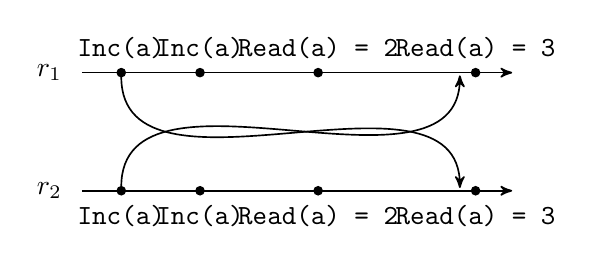
\begin{tikzpicture}[->,>=stealth',shorten >=1pt,auto,node distance=3cm,semithick, transform shape]
    
    \draw (0, 0) -- (5.5, 0);
    \draw (0, 1.5) -- (5.5, 1.5);
    
    \node[label=left:{$r_2$}] at (0, 0) {};
    \node[label=left:{$r_1$}] at (0, 1.5) {};
    
    \node[draw,circle,fill=black,scale=0.3,label=below:{\texttt{Inc(a)}}](r21) at (.5, 0) {};
    \node[draw,circle,fill=black,scale=0.3,label=below:{\texttt{Inc(a)}}](r22) at (1.5, 0) {};
    \node[draw,circle,fill=black,scale=0.3,label=below:{\texttt{Read(a) = 2}}](r23) at (3, 0) {};
    \node[draw,circle,fill=black,scale=0.3,label=below:{\texttt{Read(a) = 3}}](r24) at (5, 0) {};
    
    \node[draw,circle,fill=black,scale=0.3,label=above:{\texttt{Inc(a)}}](r11) at (.5, 1.5) {};
    \node[draw,circle,fill=black,scale=0.3,label=above:{\texttt{Inc(a)}}](r12) at (1.5, 1.5) {};
    \node[draw,circle,fill=black,scale=0.3,label=above:{\texttt{Read(a) = 2}}](r13) at (3, 1.5) {};
    \node[draw,circle,fill=black,scale=0.3,label=above:{\texttt{Read(a) = 3}}](r14) at (5, 1.5) {};
    
    \draw (r11) edge[out=-90,in=90] (4.8, 0);
    \draw (r21) edge[out=90,in=-90] (4.8, 1.5);
    
    \end{tikzpicture}  
    \caption{An admissible execution of replicated counter which will not be explored by algorithm \ref{countercrdtalgo:main}}
    \label{correction:fig1}
    \end{minipage}

    \begin{minipage}{\textwidth}
        \centering
        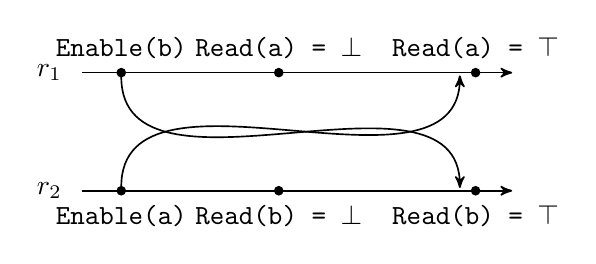
\begin{tikzpicture}[->,>=stealth',shorten >=1pt,auto,node distance=3cm,semithick, transform shape]
    
        \draw (0, 0) -- (5.5, 0);
        \draw (0, 1.5) -- (5.5, 1.5);
        
        \node[label=left:{$r_2$}] at (0, 0) {};
        \node[label=left:{$r_1$}] at (0, 1.5) {};
        
        \node[draw,circle,fill=black,scale=0.3,label=below:{\texttt{Enable(a)}}](r21) at (.5, 0) {};
        \node[draw,circle,fill=black,scale=0.3,label=below:{\texttt{Read(b) = $\bot$}}](r23) at (2.5, 0) {};
        \node[draw,circle,fill=black,scale=0.3,label=below:{\texttt{Read(b) = $\top$}}](r24) at (5, 0) {};
        
        \node[draw,circle,fill=black,scale=0.3,label=above:{\texttt{Enable(b)}}](r11) at (.5, 1.5) {};
        \node[draw,circle,fill=black,scale=0.3,label=above:{\texttt{Read(a) = $\bot$}}](r13) at (2.5, 1.5) {};
        \node[draw,circle,fill=black,scale=0.3,label=above:{\texttt{Read(a) = $\top$}}](r14) at (5, 1.5) {};
        
        \draw (r11) edge[out=-90,in=90] (4.8, 0);
        \draw (r21) edge[out=90,in=-90] (4.8, 1.5);
        
        \end{tikzpicture}  
        \caption{An admissible execution of replicated flags which will not be explored by algorithm proposed in subsection \ref{sec:ptime:sets}}
        \label{correction:fig2}
    \end{minipage}
    \end{figure}

Consider the history of a replicated counter given in figure \ref{correction:fig1}. This execution will not be explored by the algorithm \ref{countercrdtalgo:main}. This history has only one possible execution, presented in the figure. $[\mathrm{Inc}(a)]_{r_1}$ must be propagate after $[\mathrm{Read}(a) = 2]_{r_2}$ and before $[\mathrm{Read}(a) = 3]_{r_2}$. To simulate that, the algorithm must reach a prefix map which had $[\mathrm{Inc}(a)]_{r_1}$ and $[\mathrm{Read}(a) = 2]_{r_2}$ as the $\ro$-maximal operations from each replica. But the same argument holds when $[\mathrm{Inc}(a)]_{r_2}$ needs to propagate after $[\mathrm{Read}(a) = 2]_{r_1}$ and before $[\mathrm{Read}(a) = 3]_{r_1}$. So the algorithm must reach another prefix map which had $[\mathrm{Inc}(a)]_{r_2}$ and $[\mathrm{Read}(a) = 2]_{r_1}$ as the $\ro$-maximal operations from each replica.

Now the algorithm always extends the maintained prefix map \ie when successful, the valid extensions of the empty prefix map are related by inclusion. But these two prefix-maps are not \emph{related} by inclusion. So no valid extensions of prefix map will see both of them together, and the algorithm will return unsuccessfully because $\mathrm{Read}(a) = 3$ will be unsuccessful. We present a similar history for sets, flags or registers, and argue the same.

We realized, to construct $\hb$ incrementally, we need to propagate the partial $\hb$ at future operations arbitrarily at each replica. Naively, this requires maintaining a prefix map at each \textrm{Read} operation. Although the number of possible prefix map is polynomially bound for a bounded number of replicas, maintaining $n$ prefix maps at each \textrm{Read} where $n$ is in the order of the size of the history, creates exponentially many possible states to explore.

We could not find any solution to our mistake. The complexity of the admissibility problem for Counters with a bounded number of replica stays open.
  %!TEX root = ../../Thesis.tex

\section{Related Work}
\label{sec:crdt:related}

Many have considered consistency models applicable to CRDTs, including causal consistency~\cite{DBLP:journals/cacm/Lamport78}, sequential consistency~\cite{DBLP:journals/tc/Lamport79}, linearizability~\cite{DBLP:journals/toplas/HerlihyW90}, session consistency~\cite{DBLP:conf/pdis/TerryDPSTW94}, eventual consistency~\cite{DBLP:conf/sosp/TerryTPDSH95}, and happens-before consistency~\cite{DBLP:conf/popl/MansonPA05}. Burckhardt et al.~\cite{DBLP:journals/ftpl/Burckhardt14, DBLP:conf/popl/BurckhardtGYZ14} propose a unifying framework to formalize these models. Many have also studied the complexity of verifying data-type agnostic notions of consistency, including serializability, sequential consistency, and linearizability~\cite{DBLP:journals/jacm/Papadimitriou79b, DBLP:journals/siamcomp/GibbonsK97, DBLP:journals/iandc/AlurMP00, DBLP:conf/spaa/BinghamCH03, DBLP:conf/cav/FarzanM08, DBLP:conf/esop/BouajjaniEEH13, DBLP:conf/netys/Hamza15}, as well as causal consistency~\cite{DBLP:conf/popl/BouajjaniEGH17}. Our definition of the replicated LWW register corresponds to the notion of causal convergence in~\cite{DBLP:conf/popl/BouajjaniEGH17}. This work studies the complexity of the admissibility problem for the replicated LWW register. It shows that this problem is NP-complete in general and polynomial time when each value is written only once. 
Our NP-completeness result is stronger since it assumes a fixed number of replicas, and our algorithm for the case of unique values is more general and can be applied uniformly to MVR and RGA. 
While Bouajjani et al.~\cite{DBLP:journals/iandc/BouajjaniEEH18, DBLP:journals/pacmpl/EmmiE18} considers the complexity for individual linearizable collection types, we are the first to establish (in)tractability of individual replicated data types. Others have developed effective consistency checking algorithms for sequential consistency~\cite{DBLP:conf/cav/HenzingerQR99a, DBLP:journals/tpds/Qadeer03, DBLP:conf/cav/BinghamCHQZ04, DBLP:conf/pldi/BurckhardtAM07}, serializability~\cite{DBLP:conf/fmcad/0002OPTZ07, DBLP:conf/cav/FarzanM08, DBLP:conf/pldi/GuerraouiHJS08, DBLP:conf/pldi/EmmiMM10}, linearizability~\cite{DBLP:journals/jpdc/WingG93, DBLP:conf/pldi/BurckhardtDMT10, DBLP:conf/pldi/EmmiEH15, DBLP:journals/concurrency/Lowe17}, and even weaker notions like eventual consistency~\cite{DBLP:conf/popl/BouajjaniEH14} and sequential happens-before consistency~\cite{DBLP:conf/cav/EmmiE18, DBLP:journals/pacmpl/EmmiE19}. 
In contrast, we are the first to establish precise polynomial-time algorithms for runtime verification of replicated data types.

  %!TEX root = Thesis.tex
\section{Conclusion}
\label{sec:conclusion}

By developing novel logical characterizations of replicated data types, reductions from propositional satisfiability checking, and tractable algorithms, we have established a frontier of tractability for checking consistency of replicated data types. As far as we are aware, our results are the first to characterize the asymptotic complexity consistency checking for CRDTs.


  \chapter{Checking Transactional Consistency}
  \label{chap:txn}

  %!TEX root = ../../Thesis.tex

%\section{Introduction}

%Transactions simplify concurrent programming by enabling computations on shared data that are isolated from other concurrent computations and resilient to failures. Modern databases provide transactions in various forms corresponding to different tradeoffs between consistency and availability. The strongest level of consistency is achieved with \emph{serializable} transactions~\cite{DBLP:journals/jacm/Papadimitriou79b} whose outcome in concurrent executions is the same as if the transactions were executed atomically in some order. Unfortunately, serializability carries a significant penalty on the availability of the system assuming, for instance, that the database is accessed over a network that can suffer from partitions or failures. For this reason, modern databases often provide weaker guarantees about transactions, formalized by weak consistency models, e.g., causal consistency~\cite{DBLP:journals/cacm/Lamport78} and snapshot isolation~\cite{DBLP:conf/sigmod/BerensonBGMOO95}.
%
%Implementations of large-scale databases providing transactions are difficult to build and test. For instance, distributed (replicated) databases must account for partial failures, where some components or the network can fail and produce incomplete results. Ensuring fault-tolerance relies on intricate protocols that are difficult to design and reason about. The black-box testing framework Jepsen~\cite{jepsen} found a remarkably large number of subtle problems in many production distributed databases. %\footnote{https://www.infoq.com/presentations/partitioning-comparison}.
%
%Testing a transactional database raises two issues: (1) deriving a suitable set of testing scenarios, e.g., faults to inject into the system and the set of transactions to be executed, and (2) deriving efficient algorithms for checking whether a given execution satisfies the considered consistency model. The Jepsen framework aims to address the first issue by using randomization, 
%%shows that the first issue can be solved using randomization, 
%e.g., introducing faults at random and choosing the operations in a transaction randomly. The effectiveness of this approach has been proved formally in recent work~\cite{DBLP:journals/pacmpl/OzkanMNBW18}. The second issue is, however, largely unexplored. Jepsen checks consistency in a rather ad-hoc way, focusing on specific classes of violations to a given consistency model, e.g., dirty reads (reading values from aborted transactions). This problem is challenging because the consistency specifications are non-trivial and they cannot be checked using, for instance, standard local assertions added to the client's code. 
%
%Besides serializability, the complexity of checking correctness of an execution w.r.t. some consistency model is unknown. Checking serializability has been shown to be NP-complete~\cite{DBLP:journals/jacm/Papadimitriou79b}, and checking causal consistency in a \emph{non-transactional} context is known to be polynomial time~\cite{DBLP:conf/popl/BouajjaniEGH17}. In this work, we try to fill this gap by investigating the complexity of this problem w.r.t. several consistency models and, in the case of NP-completeness, devising algorithms that are polynomial time assuming fixed bounds for certain parameters of the input executions, e.g., the number of sessions. 

%
%The only result that explores the complexity of this problem 
%
%Except for  serializability, in which case it has been shown that checking  be NP-complete~\cite{DBLP:journals/jacm/Papadimitriou79b}
%% testing, i.e., randomly choosing the faults injected into the system and the transactions to be executed is enough to reveal a
%
%
%The success of Jepsen relies on random transactions as well as randomly introduced partition faults, therefore it is solved. We tackle the second issue for a series of consistency models (Jepsen implements a test of linearizability https://github.com/jepsen-io/knossos and an ad-hoc test for causal consistency restricted to bounded executions, \url{https://github.com/jepsen-io/jepsen/blob/f345226dba1266bc37487d734a02caddf7d1d125/jepsen/src/jepsen/tests/causal.clj})
In this chapter, we consider the issue of automated testing for transactional databases. More precisely, we focus on the complexity of checking correctness of an execution w.r.t. some transactional consistency model. We consider several consistency models that are the most prevalent in practice: \emph{Read Committed} (RC)~\cite{DBLP:conf/sigmod/BerensonBGMOO95}, \emph{Read Atomic} (RA)~\cite{DBLP:conf/concur/Cerone0G15}, \emph{Causal Consistency} (CC)~\cite{DBLP:journals/cacm/Lamport78}, \emph{Prefix Consistency} (PC)~\cite{DBLP:conf/ecoop/BurckhardtLPF15}, \emph{Snapshot Isolation} (SI)~\cite{DBLP:conf/sigmod/BerensonBGMOO95}, and Serializability (SER)~\cite{DBLP:journals/jacm/Papadimitriou79b}. In case of intractability, we introduce algorithms that are polynomial time assuming fixed bounds for certain parameters of the input executions, e.g., the number of sessions. 

%We consider several consistency models that are the most prevalent in practice. The weakest of them, \emph{Read Committed} (RC)~\cite{DBLP:conf/sigmod/BerensonBGMOO95}, requires that every value read in a transaction is written by a committed transaction. \emph{Read Atomic} (RA)~\cite{DBLP:conf/concur/Cerone0G15} requires that successive reads of the same variable in a transaction return the same value (also known as Repeatable Reads~\cite{DBLP:conf/sigmod/BerensonBGMOO95}), and that a transaction ``sees'' the values written by previous transactions in the same session. In general, we assume that transactions are organized in \emph{sessions}~\cite{DBLP:conf/pdis/TerryDPSTW94}, an abstraction of the sequence of transactions performed during the execution of an application.
%\emph{Causal Consistency} (CC)~\cite{DBLP:journals/cacm/Lamport78} requires that if a transaction~$\tr_1$ ``affects'' another transaction $\tr_2$, e.g., $\tr_1$ is ordered before $\tr_2$ in the same session or $\tr_2$ reads a value written by $\tr_1$, then these two transactions are observed by any other transaction in this order. \emph{Prefix Consistency} (PC)~\cite{DBLP:conf/ecoop/BurckhardtLPF15} requires that there exists a total commit order between all the transactions such that each transaction observes a prefix of this sequence. \emph{Snapshot Isolation} (SI)~\cite{DBLP:conf/sigmod/BerensonBGMOO95} further requires that two different transactions observe different prefixes if they both write to a common variable.
%%Two different transactions $\tr_1$ and $\tr_2$ may observe the same prefix, which is not allowed under \emph{Snapshot Isolation} (SI)~\cite{DBLP:conf/sigmod/BerensonBGMOO95} when these two transactions write on a common variable. 
%Finally, we also provide new results concerning the problem of checking serializability (SER) that complement the known result about its NP-completeness. 

The algorithmic issues we explore in this chapter have led to a new specification framework for these consistency models that relies on the fact that the \emph{write-read} relation in an execution (also known as \emph{read-from}), relating reads with the transactions that wrote their value, can be defined effectively. The write-read relation can be extracted easily from executions where each value is written at most once (a variable can be written an arbitrary number of times). This can be easily enforced by tagging values with unique identifiers (e.g., a local counter that is incremented with every new write coupled with a client/session identifier)\footnote{This is also used in Jepsen, e.g., checking dirty reads in Galera~\cite{jepsen-galera}.}. Since practical database implementations are data-independent~\cite{DBLP:conf/popl/Wolper86}, i.e., their behavior doesn't depend on the concrete values read or written in the transactions, any potential buggy behavior can be exposed in executions where each value is written at most once. Therefore, this assumption is without loss of generality.

Previous work~\cite{DBLP:conf/popl/BouajjaniEGH17,DBLP:conf/popl/BurckhardtGYZ14,DBLP:conf/concur/Cerone0G15} has formalized such consistency models using two auxiliary relations: a \emph{visibility} relation defining for each transaction the set of transactions it observes, and a \emph{commit order} defining the order in which transactions are committed to the ``global'' memory. An execution satisfying some consistency model is defined as the existence of a visibility relation and a commit order obeying certain axioms. In our case, the write-read relation derived from the execution plays the role of the visibility relation. This simplification allows us to state a series of axioms defining these consistency models, which have a common shape. Intuitively, they define lower bounds on the set of transactions $\tr_1$ that \emph{must} precede in commit order a transaction $\tr_2$ that is read in the execution. Besides shedding a new light on the differences between these consistency models, these axioms are essential for the algorithmic issues we investigate afterwards.

%Based on our formalization of these criteria, 
We establish the precise complexity for checking whether an execution satisfies RC, RA, or CC is polynomial time, while the same problem is NP-complete for PC and SI. Moreover, in the case of the NP-complete consistency models (PC, SI, SER), we show that their verification problem becomes polynomial time provided that, roughly speaking, the number of sessions in the input executions is considered to be fixed (i.e., not counted for in the input size). We extend these results even further by relying on an abstraction of executions called \emph{communication graphs}~\cite{DBLP:journals/pacmpl/ChalupaCPSV18}. Roughly speaking, the vertices of a communication graph correspond to sessions, and the edges represent the fact that two sessions access (read or write) the same variable. We show that all these criteria are polynomial-time checkable provided that the \emph{biconnected} components of the communication graph are of fixed size.

We provide an experimental evaluation of our algorithms on executions of CockroachDB~\cite{cockroach}, which claims to implement serializability~\cite{cockroach-claim} acknowledging however the possibility of anomalies, Galera~\cite{galera}, whose documentation contains contradicting claims about whether it implements snapshot isolation~\cite{galera-claim,galera-notclaim}, and AntidoteDB~\cite{antidote}, which claims to implement causal consistency~\cite{antidote-claim}.
%Galera~\cite{galera}, and AntidoteDB~\cite{antidote}, which claim to implement serializability~\cite{cockroach-claim}, snapshot isolation~\cite{galera-claim} and causal consistency~\cite{antidote-claim}, respectively (in the default configuration). 
Our implementation reports violations of these criteria in all cases. 
%In the case of CockroachDB, the documentation admits possible anomalies while in the case of Galera we confirm an open issue submitted on Github~\cite{galera-issue}. 
The consistency violations we found for AntidoteDB are novel and have been confirmed by its developers. We show that our algorithms are efficient and scalable.
%and they outperform an encoding to boolean satisfiability of the consistency models. 
In particular, we show that, although the asymptotic complexity of our algorithms is exponential in general (w.r.t. the number of sessions), the worst-case behavior is not exercised in practice.

The remainder of this chapter is organized as follows:
\begin{itemize}

  \item Section~\ref{sec:def} defines a new specification framework for describing common transactional-consistency criteria;

  \item Section~\ref{sec:general} shows that checking RC, RA, and CC is polynomial time while checking PC and SI is NP-complete;

  \item Section~\ref{sec:bounded_width} and Section~\ref{sec:communication} show that PC, SI, and SER are polynomial-time checkable assuming that the communication graph of the input execution has fixed-size biconnected components;
  
  \item Section~\ref{sec:exp} describes an empirical evaluation of our algorithms on executions generated by production databases;
\end{itemize}

Section~\ref{sec:trans:related} overviews related work, and Section~\ref{sec:trans:conclusion} concludes.


%a simple and effective specification methodology for weakly-consistent operations which is applicable to modern platforms like Java and C++. Furthermore, they outline the foundational principles for developing weak-consistency specification mechanisms for other platforms, to which alternate consistency models may apply. To the best of our knowledge, we are the first to develop a generic methodology capable of specifying arbitrary software APIs with operations of varying consistencies, despite their prevalence in practice, e.g., in Java.

%Aside from the sections mentioned above, we end by discussing related work and conclusions in Sections~\ref{sec:related} and~\ref{sec:conclusion}.







% \subsection{definition}

%Parallel programs use shared variables in multiple concurrent computations. Using shared variables in multiple computations may lead to unexpected behavior. Transactions are introduced to solve that problem. A transaction does a computation on variables such that progress of the transaction remains isolated from the other concurrent computation in the program. They are commonly offered by databases.
%
%Usually, the programmer wants strong guarantees about the isolation of computations in each transaction, which can be formalized in terms of serialization. But, ensuring serialization introduces severe performance reduction. This is why transaction systems offer weaker isolation guarantees, which are formalized as weak consistency models. Snapshot isolation is most popular of them all. It is implemented by the major distributed database systems, such as MS SQL Server, Oracle, Galera etc.
%
%Although, the idea of the transaction is very simple, ensuring a perfectly safe transaction system is challenging. So it is imperative that we have a way of verifying them.

%  %!TEX root = Thesis.tex

\section{Overview}

% EXPLAIN HISTORIES (HOW THEY REPRESENT EXECUTIONS)

When a client sends a transactional request to a database, typically she receives an update to the request, \eg for a write request, she may receive \textsf{true} or \textsf{false} representing whether the database was able to make the changes. To process that request, the database may need to do very complicated work - there can be parallel requests or the data may need to be replicated in different locations. But to a client's perspective, the database should simply behave in a way, as if all requests are committed to the database in a \textit{meaningful} sequence which is   \textit{consistent} to what she saw.

Whatever the clients saw, we call it a History. Given a history, we try to see if the database behaved in a way where the \textit{commit sequence} is \textit{consistent} to the History. We call a history and its possible commit sequence an Execution.

% EXPLAIN CONSISTENCY CRITERIA (THROUGH EXAMPLES)
When we say, the execution is consistent, we mean, the commit sequence satisfies some \textit{criteria} with the history. A programmer may want to have all the transactions to be committed in series - Serializability. But in practical, a programmer usually only need something weak, \eg Read Committed, Snapshot Isolation - but it depends on what kind of behavior the programmer expects.

% TODO: refine examples - make them better and not boring.
% TODO: add figures

%!TEX root = ../../Thesis.tex


\begin{table*}

 \begin{tabular}{|c|c|}
  \hline & \\
  
  \begin{subfigure}{0.45\textwidth}
   \centering
   \scalebox{0.8}{
    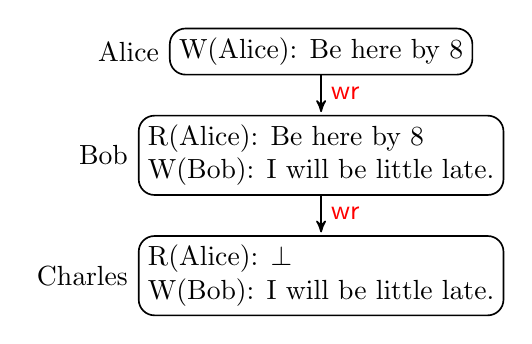
\begin{tikzpicture}[->,>=stealth',shorten >=1pt,auto,node distance=.5cm,
      semithick, transform shape]
     \node[draw, rounded corners=2mm, label=left:{Alice}] (alice) {W(Alice): Be here by 8};
     \node[draw, rounded corners=2mm, align=left, label=left:{Bob}, below = of alice] (bob) {R(Alice): Be here by 8\\ W(Bob): I will be little late.};
     \node[draw, rounded corners=2mm, align=left, label=left:{Charles}, below = of bob] (charles) {R(Alice): $\bot$\\ W(Bob): I will be little late.};
     \draw  (alice) edge node{$\wro$} (bob);
     \draw  (bob) edge node{$\wro$} (charles);
    \end{tikzpicture}
   }
   \caption{Causal violation}
   \label{causal_violation_demo}
  \end{subfigure}
  
         &        
  
  \begin{subfigure}{0.45\textwidth}
   \centering
   \scalebox{0.8}{
    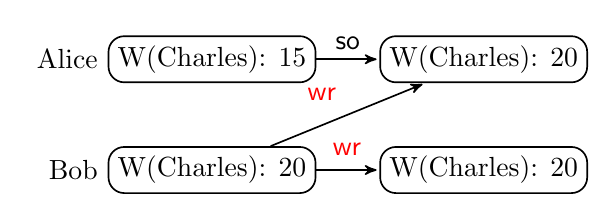
\begin{tikzpicture}[->,>=stealth',shorten >=1pt,auto,node distance=.8cm,
      semithick, transform shape]
     \node[draw, rounded corners=2mm, label=left:{Alice}] (alice1) {W(Charles): 15};
     \node[draw, rounded corners=2mm, right = of alice1] (alice2) {W(Charles): 20};
     \node[draw, rounded corners=2mm, label=left:{Bob}, below = of alice1] (bob1) {W(Charles): 20};
     \node[draw, rounded corners=2mm, below = of alice2] (bob2) {W(Charles): 20};
     \draw  (alice1) edge node{$\so$} (alice2);
     \draw  (bob1) edge node{$\wro$} (bob2);
     \draw  (bob1) edge node{$\wro$} (alice2);
    \end{tikzpicture}
    }
   \caption{Lost update}
   \label{lost_update_demo}
  \end{subfigure}
  
         \\ \hline & \\
  
  \begin{subfigure}{0.45\textwidth}
   \centering
   \scalebox{0.8}{
    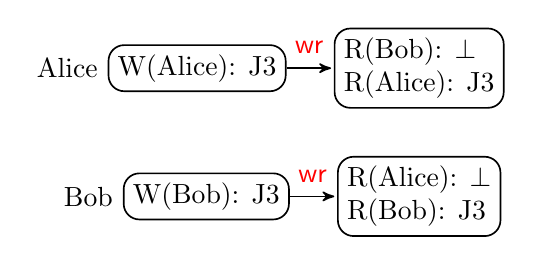
\begin{tikzpicture}[->,>=stealth',shorten >=1pt,auto,node distance=.6cm,
      semithick, transform shape]
     \node[draw, rounded corners=2mm, label=left:{Alice}] (alice1) {W(Alice): J3};
     \node[draw, rounded corners=2mm, right = of alice1, align=left] (alice2) {R(Bob): $\bot$\\ R(Alice): J3};
     \node[draw, rounded corners=2mm, below = of alice2,align=left] (bob2) {R(Alice): $\bot$\\ R(Bob): J3};
     \node[draw, rounded corners=2mm, label=left:{Bob}, left = of bob2] (bob1) {W(Bob): J3};
     \draw  (alice1) edge node{$\wro$} (alice2);
     \draw  (bob1) edge node{$\wro$} (bob2);
    \end{tikzpicture}
    }
   \caption{Long Fork}
   \label{long_fork_demo}
  \end{subfigure}
  
         &        
  
  \begin{subfigure}{0.45\textwidth}
   \centering
   \scalebox{0.8}{
    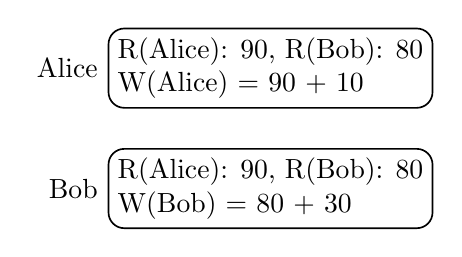
\begin{tikzpicture}[->,>=stealth',shorten >=1pt,auto,node distance=.5cm,
      semithick, transform shape]
     \node[draw, rounded corners=2mm, label=left:{Alice}, align=left] (alice1) {R(Alice): 90, R(Bob): 80\\ W(Alice) = 90 + 10};
     \node[draw, rounded corners=2mm, label=left:{Bob}, align=left,below = of alice1] (bob1) {R(Alice): 90, R(Bob): 80\\ W(Bob) = 80 + 30};
    \end{tikzpicture}
    }
   \caption{Write Skew}
   \label{write_skew_demo}
  \end{subfigure}
  \\
  \hline
 \end{tabular}
 \caption{Anomalies in database applications}
 \label{anomalies}
\end{table*}


Let's look at some anomalies that can happen in database applications. Alice, Bob and Charles are in a Whatsapp group. Alice asks everyone to come at 8 o'clock. Bob sees it and replies, he will be late. But as illustracted in \ref{causal_violation_demo}, Charles cannot see Alice's message but sees Bob's message and thinks Bob is saying he will be late for nothing. This anomaly is called \textit{Causality Violation}.

Even such anomalies can happen in bank operations. Say Alice and Bob are trying to send money to Charles. Alice sends \$15 and Bob sends \$20. But as illustrated in \ref{lost_update_demo}, Alice's deposit is lost. This anomaly is called \textit{Lost Update}.

Suppose Alice and Bob trying to book a cinema ticket. First Alice and Bob both publish they want to book a seat and check the response of other person so that they know they have a conflict. But as illustrated in \ref{long_fork_demo}, they can't see each other's reponse and ends up booking the same seat. This anomaly is called \textit{Long Fork}. 

Consider Amazon is giving out cashback for purchases. But it has to also check sum of total cashback is not more than \$200 before giving away a cashback. Otherwise, it may end up giving away too much cashback to make profit. So if Alice and Bob both become eligible for a cashback, as illustrated in \ref{write_skew_demo}, even if the total cashback value crosses the limit, the situation can let both of them have the cashback. This anomaly is called \textit{Write Skew}.

Modern databases support different levels of consistency, allowing the programmer to modify the isolation level according to her concurrent and consistency need.

% ROADMAP OF THE DIFFERENT ALGORITHMS/COMPLEXITY RESULTS (FIXED NUMBER OF SESSIONS)
First we will formally define history. Then we will define some consistency axioms and criteria over history. Then we deduce the complexity classes to verify history against respective consistency criteria. We will see Serializability, Snapshot Isolation and Prefix consistency are in NP-Complete. Then we will show for fixed number of sessions, the respective problems are in NL complexity class.

% EXPLAIN COMMUNICATION GRAPHS  

  %!TEX root = ../../Thesis.tex

\section{Consistency Criteria}\label{sec:def}

\subsection{Histories}


% \begin{table*}
%  \centering
%  \resizebox{\textwidth}{!}{
%   \begin{tabular}{ |c c|c c|c c|c c|}
%    \hline
%    \multicolumn{7}{|c}{
%     \shortstack{
%      $\forall (O, \textsf{po}) \in \mathcal{T}, \forall o \in O, o = read(x, n) \wedge \left\{o' \in \textsf{po}^{-1}(o) \mid o' = \_(x, \_) \right\} \neq \emptyset \Rightarrow$ \\
%      $max_{\textsf{po}} \left(\left\{o' \in \textsf{po}^{-1}(o) \mid o' = \_(x, \_) \right\}\right) = \_(x, n)$
%     }
%    }                    & {\textsc{(Int)}}                                                                                                                                        \\
%    \hline
%    \multicolumn{7}{|c}{
%     \shortstack{
%      $\forall T = (O, \textsf{po}) \in \mathcal{T}, \forall x, T \models \texttt{read}(x, n) \Rightarrow max_{\CO} \left(\VIS^{-1}(T) \cap \textsf{Write}_x\right) \models \texttt{write}(x, n)$
%     }
%    }                    & {\textsc{(Ext)}}                                                                                                                                        \\
%    \hline
%    $\SO \subseteq \VIS$ & \textsc{(Session)}      & \VIS is transitive & \textsc{(TransVis)} & $\CO;\VIS \subseteq \VIS$ & \textsc{(Prefix)} & $\VIS = \CO$ & \textsc{(TotalVis)} \\
%    \hline
%    \multicolumn{7}{|c}{
%     $\forall T, S \in \mathcal{T}, \forall x, (T, S \in \textsf{Write}_x \wedge T \neq S) \Rightarrow (T \xrightarrow{\VIS} S \vee S \xrightarrow{\VIS} T)$
%    }                    & {\textsc{(NoConflict)}}                                                                                                                                 \\
%    \hline
%   \end{tabular}
%  }
%  \caption{Consistency axioms, declaring behaviors on schedule}
%  \label{weakconsistency:1}
% \end{table*}



We consider a transactional database storing a set of variables $\Var=\{\xvar,\yvar,\ldots\}$. Clients interact with the database by issuing transactions formed of $\textsf{read}$ and $\textsf{write}$ operations. Assuming an unspecified set of values $\Val$ and a set of operation identifiers $\OId$, we let 
\begin{align*}
 \Op=\set{\rd[\id]{\xvar}{\val},\wrt[\id]{\xvar}{\val}: \id\in\OId, \xvar\in\Var, \val\in \Val}
\end{align*} 
be the set of operations reading a value $\val$ or writing a value $\val$ to a variable $\xvar$. We omit operation identifiers when they are not important.

\begin{definition}
 A \emph{transaction log} $\tup{\tr, O, \po}$ is a transaction identifier $\tr$ and a finite set of operations $O$ along with a strict total order $\po$ on $O$, called \emph{program order}.
\end{definition}

The program order $\po$ represents the order between instructions in the body of a transaction. We assume that each transaction log is well-formed in the sense that if a read of a key $\xvar$ is preceded by a write to $\xvar$ in $\po$, then it should return the value written by the last write to $\xvar$ before the read (w.r.t. $\po$). This property is implicit in the definition of every isolation level that we are aware of. For simplicity, we may use the term \emph{transaction} instead of transaction log and ignore transaction identifier assuming all transaction is uniquely identified. The  set of all transaction logs is denoted by $\mathsf{Tlogs}$.

We use $\tr$, $\tr_1$, $\tr_2$, $\ldots$ to range over transactions. The set of read, resp., write, operations in a transaction $\tr$ is denoted by $\readOp{\tr}$, resp., $\writeOp{\tr}$. The extension to sets of transactions is defined as usual. Also, we say that a transaction $\tr$ \emph{writes} a variable $\xvar$, denoted by $\writeVar{\tr}{\xvar}$, when $\wrt[\id]{\xvar}{\val}\in \writeOp{\tr}$ for some $\id$ and $\val$. Similarly, a transaction $\tr$ \emph{reads} a variable $\xvar$ when $\rd[\id]{\xvar}{\val}\in \readOp{\tr}$ for some $\id$ and $\val$.

\begin{figure}[t]
 \centering
 \begin{subfigure}{.21\textwidth}
   \centering
  \resizebox{!}{1.3cm}{
   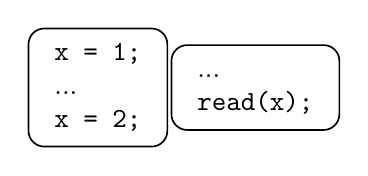
\begin{tikzpicture}[->,>=stealth',shorten >=1pt,auto,node distance=2cm,
     semithick, transform shape]
    \node[draw, rounded corners=2mm] (t1) {\begin{tabular}{l} \texttt{x = 1;} \\ ... \\ \texttt{x = 2;} \end{tabular}};
    \node[draw, rounded corners=2mm, right of = t1] (t2) {\begin{tabular}{l} ... \\ \texttt{read(x);} \end{tabular}};
   \end{tikzpicture}  
  }
%  \caption{Only the lastest write is visible to other transaction}
\caption{}
  \label{rc_eg:1}
 \end{subfigure}
 \hspace{10mm}
 \begin{subfigure}{.1\textwidth}
   \centering
  \resizebox{!}{2cm}{
   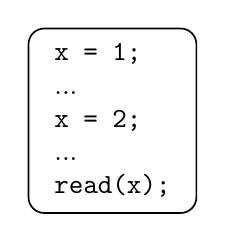
\begin{tikzpicture}[->,>=stealth',shorten >=1pt,auto,node distance=2cm,
     semithick, transform shape]
    \node[draw, rounded corners=2mm] (t1) {\begin{tabular}{l} \texttt{x = 1;} \\ ... \\ \texttt{x = 2;} \\ ... \\ \texttt{read(x);}\end{tabular}};
   \end{tikzpicture}  
  }
%  \caption{Always reads the latest write inside a transaction}
\caption{}
  \label{rr_eg:1}
 \end{subfigure}
 \hspace{10mm}
 \begin{subfigure}{.14\textwidth}
   \centering
  \resizebox{!}{1.3cm}{
   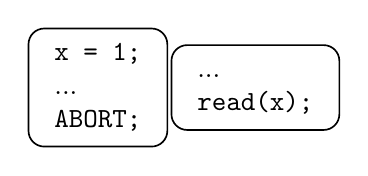
\begin{tikzpicture}[->,>=stealth',shorten >=1pt,auto,node distance=2cm,
     semithick, transform shape]
    \node[draw, rounded corners=2mm] (t1) {\begin{tabular}{l} \texttt{x = 1;} \\ ... \\ \texttt{ABORT;} \end{tabular}};
    \node[draw, rounded corners=2mm, right of = t1] (t2) {\begin{tabular}{l} ... \\ \texttt{read(x);} \end{tabular}};
   \end{tikzpicture}  
  }
%  \caption{Aborted transactions are not visible}
\caption{}
  \label{abort:1}
 \end{subfigure}
 \caption{Examples of transactions used to justify our simplifying assumptions (each box represents a different transaction): (a) only the last written value is observable in other transactions, (b) reads following writes to the same variable return the last written value in the same transaction, and (c) values written in aborted transactions are not observable.}
 \label{read_latest}
 \vspace{-3mm}
\end{figure}

To simplify the exposition, we assume that each transaction $\tr$ contains at most one write operation to each variable\footnote{That is, for every transaction $\tr$, and every $\wrt{\xvar}{\val}, \wrt{\yvar}{\val'}\in \writeOp{\tr}$, we have that $\xvar\neq\yvar$.}, and that a read of a variable $\xvar$ cannot be preceded by a write to $\xvar$ in the same transaction\footnote{That is, for every transaction $\tr=\tup{O, \po}$, if $\wrt{\xvar}{\val}\in \writeOp{\tr}$ and there exists $\rd{\xvar}{\val}\in \readOp{\tr}$, then we have that $\tup{\rd{\xvar}{\val},\wrt{\xvar}{\val}}\in \po$}. If a transaction would contain multiple writes to the same variable, then only the last one should be visible to other transactions (w.r.t. any consistency criterion considered in practice). For instance, the \texttt{read(x)} in Figure~\ref{rc_eg:1} should not return 1 because this is not the last value written to {\tt x} by the other transaction. It can return the initial value or 2.
%In figure (\ref{rc_eg:1}), however the two transactions are executed, the operation \texttt{print(x)} in below transaction should not print \texttt{0}. Because \texttt{x=0} is not the latest write in the above transaction.
Also, if a read would be preceded by a write to the same variable in the same transaction, then it should return a value written in the same transaction (i.e., the value written by the latest write to $\xvar$ in that transaction). 
For instance, the \texttt{read(x)} in Figure~\ref{rr_eg:1} can only return 2 (assuming that there are no other writes on {\tt x} in the same transaction).
%In figure (\ref{rr_eg:1}), the operation \texttt{print(x)} in the transaction should not print \texttt{1}, because $\texttt{print(x)}$ is not the latest write to \texttt{print(x)}.
These two properties can be verified easily (in a syntactic manner) on a given execution. Beyond these two properties, the various consistency criteria used in practice constrain only the last writes to each variable in each transaction and the reads that are not preceded by writes to the same variable in the same transaction.

Consistency criteria are formalized on an abstract view of an execution called~\emph{history}. A history includes only successful or committed transactions. In the context of databases, it is always assumed that the effect of aborted transactions should not be visible to other transactions, and therefore, they can be ignored. For instance, the \texttt{read(x)} in Figure~\ref{abort:1} should not return the value 1 written by the aborted transaction. The transactions are ordered according to a (partial) \emph{session order} $\so$ which represents ordering constraints imposed by the applications using the database. Most often, $\so$ is a union of sequences, each sequence being called a \emph{session}. We assume that the history includes a \emph{write-read} relation that identifies the transaction writing the value returned by each read in the execution. As mentioned before, such a relation can be extracted easily from executions where each value is written at most once. Since in practice, databases are data-independent~\cite{DBLP:conf/popl/Wolper86}, i.e., their behavior does not depend on the concrete values read or written in the transactions, any potential buggy behavior can be exposed in such executions. 

%Transactions and operations may be failed or aborted. The effects of the failed or aborted transactions and operations should not be visible. So we assume the transactions and operations are always successful or committed. If such transactions and operations exist, we discard them after checking there is no operation that read from failed or aborted transactions or operations. Therefore  In figure (\ref{abort:1}), the left transaction is aborted. So the operation \texttt{print(x)} in the right transaction should not output \texttt{0}. 


%We assume, in each transaction if there is no write before a read, it reads either from the last write of an another transaction or an initial value. Also when a transaction reads a value after a write, it reads from last write before that read. \ie if $\rd{\xvar}{\val} \in \tr_1$ reads from $\wrt{\xvar}{\val} \in \tr_2$, then for any other $\wrt{\xvar}{\_} \in \tr_2$ or $\tr_1$, $\tup{\wrt{\xvar}{\_}, \wrt{\xvar}{\val}} \in O_{\tr_2}$ or $\tup{\rd{\xvar}{\val}, \wrt{\xvar}{\_}} \in O_{\tr_1}$.
%
%Once we have a set of transactions, we can statically check if this is true for all transactions. Then, for all variables, we can ignore all the writes except the final one and all the reads after first write in a transaction. For simplicity, we assume that 



% TODO EXPLAIN THE FOLLOWING SIMPLIFICATIONS: WE DON'T CARE ABOUT MULTIPLE WRITES SINCE ANYWAY, ALL CRITERIA REQUIRE THAT ONLY THE LAST ONE IS VISIBLE. ALSO, ONCE A VARIABLE IS WRITTEN EVERY CRITERION REQUIRES THAT THE READ RETURNS THE INTERNALLY WRITTEN VALUE. ALL THESE THINGS CAN BE CHECKED EASILY IN A SYNTACTIC WAY ON HISTORIES.


%We say that a transaction $\tr$ writes value $\val$ a variable $\xvar$, denoted by $\tr\models \wrt{\xvar}{\val}$, whenever $\wrt{\xvar}{\val}$ is the last write o variable $\xvar$ of $\tr$, i.e., $\wrt{\xvar}{\val}\in \writeOp{\tr}$ and for any $\wrt{\xvar}{\val'}\in \writeOp{\tr}$ with $\val\neq\val'$, we have that $\tup{\wrt{\xvar}{\val'}, \wrt{\xvar}{\val}}\in \po$.
% \item $\tr \models \wrt[\id]{\xvar}{\val} \Leftrightarrow max_{\textsf{po}} \left( \left\{ write(x,\_) \in O \right\} \right) = write(x, n)$
% \item $(O, \textsf{po}) \models \texttt{read}(x, n) \Leftrightarrow min_{\textsf{po}} \left( \left\{ \_(x,\_) \in O \right\} \right) = read(x, n)$
% \item $(O, \textsf{po}) \in Write_{x} \Leftrightarrow \left\{ write(x,\_) \in O \right\} \neq \emptyset$



%When a read operation in a transaction reads a value from an operation from another transaction, it defines a \emph{write-read order} between them. Also, typically a transactional system allows its clients to group their transactions in one single session. This imposes a \emph{session order} on the transactions. We define a client-visible results of an execution of a set of sessions as a \emph{history}.

% TODO SAY THAT HISTORIES CONTAIN ONLY COMMITTED TRANSACTIONS FROM A CONCRETE EXECUTION, THE EFFECTS OF ABORTED TRANSACTIONS ARE NOT VISIBLE.

\begin{definition}
 A \emph{history} $\tup{T, \so, \wro}$ is a set of transactions $T$ along with a strict partial order $\so$ called \emph{session order}, and a 
 %surjective\footnote{That is, for all $\rd{\xvar}{\val}\in \readOp{T}$ there exists a transaction $\tr\in T$ such that $\tup{\tr,\rd{\xvar}{\val}}\in \wro$.} 
 relation $\wro\subseteq T\times \readOp{T}$ called \emph{write-read} relation, s.t. 
 \begin{itemize}
  \item the inverse of $\wro$ is a total function, and if $(\tr,\rd{\xvar}{\val})\in\wro$, then $\wrt{\xvar}{\val}\in\tr$, and
  \item $\so\cup\wro$ is acyclic.
 \end{itemize}
\end{definition}

% TODO SAY THAT INITIAL VALUES ARE ASSUMED TO BE WRITTEN BY A TRANSACTION ORDERED IN SO BEFORE ALL THE OTHER TRANSACTIONS.

%The transactions may try to read a variable, even before there is a write to it. In practice, the databases return a default initialized or null value for those reads. This situation can be thought as if the database wrote that value in an \emph{initialization} transaction, in which all variables are written with an initialized value. So we assume a history contains an initialization transaction. This initialization transaction precedes all other transactions by $\so$.

To simplify the technical exposition, we assume that every history includes a distinguished transaction writing the initial values of all variables. This transaction precedes all the other transactions in $\so$. We use $\hist$, $\hist_1$, $\hist_2$, $\ldots$ to range over histories. 

We say that the read operation $\rd{\xvar}{\val}$ reads value $\val$ from variable $\xvar$ written by $\tr$ when $(\tr,\rd{\xvar}{\val})\in\wro$. 
For a given variable $\xvar$, $\wro[\xvar]$ denotes the restriction of $\wro$ to reads of variable $\xvar$, \ie, $\wro[\xvar]=\wro\cap (T\times \{\rd{\xvar}{\val}\mid \val\in \Val\})$. Moreover, we extend the relations $\wro$ and $\wro[\xvar]$ to pairs of transactions as follows: $\tup{\tr_1,\tr_2}\in \wro$, resp., $\tup{\tr_1,\tr_2}\in \wro[\xvar]$, iff there exists a read operation $\rd{\xvar}{\val}\in \readOp{\tr_2}$ such that $\tup{\tr_1,\rd{\xvar}{\val}}\in \wro$, resp., $\tup{\tr_1,\rd{\xvar}{\val}}\in \wro[\xvar]$. We say that the transaction $\tr_1$ is \emph{read} by the transaction $\tr_2$ when $\tup{\tr_1,\tr_2}\in \wro$, and that it is \emph{read} when it is read by some transaction $\tr_2$. 
%

%A consistency model describes how a transactional system processes transactions. To formally define the behaviors, we will extend history with two relations.

%The definitions of the consistency criteria rely on a few basic notions of sequences and orders. We denote the \emph{prefix} of a sequence $\sigma$ up to and including an element $\alpha$ by $\sigma(\alpha)$, and the \emph{prefix} of a partial order $\pi$ up to and including $\alpha$ by $\pi(\alpha) = \set{\tup{ \alpha_1, \alpha_2 } \in \pi : \tup{\alpha_2, \alpha} \in \pi \text{ or } \alpha_2 = \alpha }$. A sequence $\sigma_1$ is called a \emph{subsequence} of another sequence $\sigma_2$, denoted by $\sigma_1\preceq \sigma_2$, when $\sigma_1$ is obtained from $\sigma_2$ by deleting elements. We extend the notion of subsequence to partial orders and say that an order $\pi_1$ is a \emph{suborder} of another order $\pi_2$ if $\pi_1\subseteq \pi_2$. For uniformity, we write $\pi_1 \preceq \pi_2$ when $\pi_1$ is a suborder of $\pi_2$. The subsequence of a sequence $\sigma$ that includes all the elements ordered between two elements $\alpha_1$ and $\alpha_2$ (including $\alpha_1$ and $\alpha_2$) is denoted by $\sigma[\alpha_1,\alpha_2]$.
%Also, for simplicity, we don’t make the distinction between sequences and total orders, reusing notions like prefix and subsequence in the context of total orders.
%
%\begin{definition}
% A \emph{linearization} $\ell=\tup{\lin,\vis}$ of a history $\tup{T, \so, \wro}$ is a total order $\lin$ on $T$, and a function $\vis$, mapping each transaction $\tr\in T$ to a subsequence of $\lin(\tr)$ including $\tr$.
%\end{definition}
%
%A consistency model is defined as the set of histories which admit linearizations satisfying certain \emph{consistency axioms}. The axioms rely on a few notations
%\begin{itemize}
% \item $\tr \models \wrt[\id]{\xvar}{\val} \Leftrightarrow max_{\textsf{po}} \left( \left\{ write(x,\_) \in O \right\} \right) = write(x, n)$
% \item $(O, \textsf{po}) \models \texttt{read}(x, n) \Leftrightarrow min_{\textsf{po}} \left( \left\{ \_(x,\_) \in O \right\} \right) = read(x, n)$
% \item $(O, \textsf{po}) \in Write_{x} \Leftrightarrow \left\{ write(x,\_) \in O \right\} \neq \emptyset$
%\end{itemize}


\subsection{Axiomatic Framework}

% from Table. \ref{weakconsistency:1}. Table. \ref{weakconsistency:2} lists the axioms of consistency models.

%!TEX root = Thesis.tex

\tikzset{transaction state/.style={draw=black!0}}


 \begin{figure}
   \resizebox{\textwidth}{!}{
   \footnotesize
  \begin{tabular}{|c|c|c|}
   \hline &  & \\
   \begin{subfigure}[t]{.3\textwidth}
    \centering
    \begin{tikzpicture}[->,>=stealth',shorten >=1pt,auto,node distance=1cm,
      semithick, transform shape]
     \node[transaction state, text=red] at (0,0)       (t_1)           {$\tr_1$};
     \node[transaction state, text=red, label={above:\textcolor{red}{$\writeVar{ }{\xvar}$}}] at (-0.5,1.5) (t_2) {$\tr_2$};
     \node[transaction state, text=red] at (2,0)       (o_1)           {$\alpha$};
     \node[transaction state] at (1.5,1.5) (o_2) {$\beta$};
     \path (t_1) edge[red] node {$\wro[\xvar]$} (o_1);
     % \path (t_2) edge[blue] node {$\CO$} (t_1);
     \path (t_2) edge node {$\wro$} (o_2);
     \path (o_2) edge node {$\po$} (o_1);
     \path (t_2) edge[left,double] node {$\co$} (t_1);
    \end{tikzpicture}
    \parbox{\textwidth}{
     $\forall \xvar,\ \forall \tr_1, \tr_2,\ \forall \alpha.\ \tr_1\neq \tr_2\ \land$
     
     \hspace{4mm}$\tup{\tr_1,\alpha}\in \wro[\xvar] \land \writeVar{\tr_2}{\xvar}\ \land$ 
     
     \hspace{9mm}$\tup{\tr_2,\alpha}\in\wro\circ\po$
     
     \hspace{14mm}$\implies \tup{\tr_2,\tr_1}\in\co$
    }
    %\end{align*}
    
    \caption{$\mathsf{Read\ Committed}$}
    \label{lock_rc_def}
   \end{subfigure}
   
          &     
   
   \begin{subfigure}[t]{.3\textwidth}
    \centering
    \begin{tikzpicture}[->,>=stealth',shorten >=1pt,auto,node distance=4cm,
      semithick, transform shape]
     \node[transaction state, text=red] at (0,0)       (t_1)           {$\tr_1$};
     \node[transaction state] at (2,0)       (t_3)           {$\tr_3$};
     \node[transaction state, text=red,label={above:\textcolor{red}{$\writeVar{ }{\xvar}$}}] at (-.5,1.5) (t_2) {$\tr_2$};
     \path (t_1) edge[red] node {$\wro[\xvar]$} (t_3);
     % \path (t_2) edge[blue] node {$\CO$} (t_1);
     \path (t_2) edge[bend left] node {$\wro \cup \so$} (t_3);
     \path (t_2) edge[left,double] node {$\co$} (t_1);
    \end{tikzpicture}
    \parbox{\textwidth}{
     $\forall \xvar,\ \forall \tr_1, \tr_2,\ \forall \tr_3.\ \tr_1\neq \tr_2\ \land$
     
     \hspace{4mm}$\tup{\tr_1,\tr_3}\in \wro[\xvar] \land \writeVar{\tr_2}{\xvar}\ \land$ 
     
     \hspace{9mm}$\tup{\tr_2,\tr_3}\in\wro\cup\so$
     
     \hspace{14mm}$\implies \tup{\tr_2,\tr_1}\in\co$
    }
    
    \caption{$\mathsf{Read\ Atomic}$}
    \label{ra_def}
   \end{subfigure}
   
   &
   
   \begin{subfigure}[t]{.3\textwidth}
    \centering
    \begin{tikzpicture}[->,>=stealth',shorten >=1pt,auto,node distance=4cm,
      semithick, transform shape]
     \node[transaction state, text=red] at (0,0)       (t_1)           {$\tr_1$};
     \node[transaction state] at (2,0)       (t_3)           {$\tr_3$};
     \node[transaction state, text=red,label={above:\textcolor{red}{$\writeVar{ }{\xvar}$}}] at (-.5,1.5) (t_2) {$\tr_2$};
     \path (t_1) edge[red] node {$\wro[\xvar]$} (t_3);
     % \path (t_2) edge[blue] node {$\CO$} (t_1);
     \path (t_2) edge[dashed, bend left] node {$(\wro \cup \so)^+$} (t_3);
     %   \path [->, decoration={snake}] (t_2) edge[decorate] node[auto] {F} (t_3);
     \path (t_2) edge[left,double] node {$\co$} (t_1);
    \end{tikzpicture}
    \parbox{\textwidth}{
     $\forall \xvar,\ \forall \tr_1, \tr_2,\ \forall \tr_3.\ \tr_1\neq \tr_2\ \land$
     
     \hspace{4mm}$\tup{\tr_1,\tr_3}\in \wro[\xvar] \land \writeVar{\tr_2}{\xvar}\ \land$ 
     
     \hspace{9mm}$\tup{\tr_2,\tr_3}\in(\wro\cup\so)^+$
     
     \hspace{14mm}$\implies \tup{\tr_2,\tr_1}\in\co$
    }
    
    \caption{$\mathsf{Causal}$}
    \label{cc_def}
   \end{subfigure}
   
   
   \\ \hline & & \\
    
   \begin{subfigure}[t]{.3\textwidth}
    \centering
    \begin{tikzpicture}[->,>=stealth',shorten >=1pt,auto,node distance=4cm,
      semithick, transform shape]
     \node[transaction state, text=red] at (0,0)       (t_1)           {$\tr_1$};
     \node[transaction state] at (2,0)       (t_3)           {$\tr_3$};
     \node[transaction state, text=red,label={above:\textcolor{red}{$\writeVar{ }{\xvar}$}}] at (-0.5,1.5) (t_2) {$\tr_2$};
     \node[transaction state] at (1.5,1.5) (t_4) {$\tr_4$};
     \path (t_1) edge[red] node {$\wro[\xvar]$} (t_3);
     % \path (t_2) edge[blue] node {$\CO$} (t_1);
     \path (t_2) edge node {$\co^*$} (t_4);
     \path (t_4) edge[left] node {$(\wro \cup \so)$} (t_3);
     \path (t_2) edge[left,double] node {$\co$} (t_1);
    \end{tikzpicture}
    \parbox{\textwidth}{
     $\forall \xvar,\ \forall \tr_1, \tr_2,\ \forall \tr_3.\ \tr_1\neq \tr_2\ \land$
     
     \hspace{4mm}$\tup{\tr_1,\tr_3}\in \wro[\xvar] \land \writeVar{\tr_2}{\xvar}\ \land$ 
     
     \hspace{9mm}$\tup{\tr_2,\tr_3}\in\co^*\circ\,(\wro\cup\so)$
     
     \hspace{14mm}$\implies \tup{\tr_2,\tr_1}\in\co$
    }
    
    \caption{$\mathsf{Prefix}$}
    \label{pre_def}
   \end{subfigure}
          
   
   &
   \begin{subfigure}[t]{.32\textwidth}
    \centering
    \begin{tikzpicture}[->,>=stealth',shorten >=1pt,auto,node distance=4cm,
      semithick, transform shape]
     \node[transaction state, text=red] at (0,0)       (t_1)           {$\tr_1$};
     \node[transaction state, label={below:$\writeVar{ }{\yvar}$}] at (2,0)       (t_3)           {$\tr_3$};
     \node[transaction state, text=red,label={above:\textcolor{red}{$\writeVar{ }{\xvar}$}}] at (-.5,1.5) (t_2) {$\tr_2$};
     \node[transaction state, label={above:{$\writeVar{}{\yvar}$}}] at (1.5,1.5) (t_4) {$\tr_4$};
     \path (t_1) edge[red] node {$\wro[\xvar]$} (t_3);
     % \path (t_2) edge[blue] node {$\CO$} (t_1);
     \path (t_2) edge node {$\co^*$} (t_4);
     \path (t_4) edge node {$\co$} (t_3);
     \path (t_2) edge[left,double] node {$\co$} (t_1);
    \end{tikzpicture}
    \parbox{\textwidth}{
     $\forall \xvar,\ \forall \tr_1, \tr_2,\ \forall \tr_3, \tr_4,\ \forall \yvar.\ \tr_1\neq \tr_2\ \land$
     
     \hspace{4mm}$\tup{\tr_1,\tr_3}\in \wro[\xvar] \land \writeVar{\tr_2}{\xvar}\ \land$ 
     
     \hspace{9mm}$\writeVar{\tr_3}{\yvar}\ \land \writeVar{\tr_4}{\yvar}\ \land$ 
     
     \hspace{12mm}$\tup{\tr_2,\tr_4}\in\co^*\ \land \tup{\tr_4,\tr_3}\in\co$
     
     \hspace{16mm}$\implies \tup{\tr_2,\tr_1}\in\co$
    }
    
    \caption{$\mathsf{Conflict}$}
    \label{confl_def}
   \end{subfigure}
          &     
   \begin{subfigure}[t]{.3\textwidth}
    \centering
    \begin{tikzpicture}[->,>=stealth',shorten >=1pt,auto,node distance=4cm,
      semithick, transform shape]
     \node[transaction state, text=red] at (0,0)       (t_1)           {$\tr_1$};
     \node[transaction state] at (2,0)       (t_3)           {$\tr_3$};
     \node[transaction state, text=red, label={above:\textcolor{red}{$\writeVar{ }{\xvar}$}}] at (-.5,1.5) (t_2) {$\tr_2$};
     \path (t_1) edge[red] node {$\wro[\xvar]$} (t_3);
     % \path (t_2) edge[blue] node {$\CO$} (t_1);
     \path (t_2) edge[bend left] node {$\CO$} (t_3);
     \path (t_2) edge[left,double] node {$\co$} (t_1);
    \end{tikzpicture}
    \parbox{\textwidth}{
     $\forall \xvar,\ \forall \tr_1, \tr_2,\ \forall \tr_3.\ \tr_1\neq \tr_2\ \land$
     
     \hspace{4mm}$\tup{\tr_1,\tr_3}\in \wro[\xvar] \land \writeVar{\tr_2}{\xvar}\ \land$ 
     
     \hspace{9mm}$\tup{\tr_2,\tr_3}\in\co$
     
     \hspace{14mm}$\implies \tup{\tr_2,\tr_1}\in\co$
    }
    
    \caption{$\mathsf{Serializability}$}
    \label{ser_def}
   \end{subfigure}
   \\ \hline
  \end{tabular}
  }
  \caption{Definitions of consistency axioms. The reflexive and transitive, resp., transitive, closure of a relation $rel$ is denoted by $rel^*$, resp., $rel^+$. Also, $\circ$ denotes the composition of two relations, i.e., $rel_1 \circ rel_2 = \{\tup{a, b} | \exists c. \tup{a, c} \in rel_1 \land \tup{c, b} \in rel_2\}$.}
  \label{consistency_defs}
 \end{figure}



% Practically, \textsc{Int} ensures each transaction takes one global snapshot of variables at the beginning. Then no other global changes affect that snapshot for any read or write local to that transaction. \textsc{Ext} ensures each transaction always observes the latest global snapshot that is visible to it.

We describe an axiomatic framework to characterize the set of histories satisfying a certain consistency criterion. The overarching principle is to say that a history satisfies a certain criterion if there exists a strict total order on its transactions, called \emph{commit order} and denoted by $\co$, which extends the write-read relation and the session order, and which satisfies certain properties. These properties are expressed by a set of axioms that relate the commit order with the session-order and the write-read relation in the history. 

%\begin{figure}
%  
%   \centering
%   \begin{subfigure}{.22\textwidth}
%  \resizebox{\textwidth}{!}{
%  \begin{tikzpicture}[->,>=stealth',shorten >=1pt,auto,node distance=3cm,
%    semithick, transform shape]
%    % \node[draw, rounded corners=2mm] (t1) at (0, 0) {\begin{tabular}{l} \texttt{x = 1;} \end{tabular}};
%   \node[draw, rounded corners=2mm] (t2) at (0, -.75) {\begin{tabular}{l} \texttt{x = 1;} \\ \texttt{y = 1};\end{tabular}};
%   \node[draw, rounded corners=2mm, minimum width=3.5cm, minimum height=2.5cm] (t3) at (3, -0.75) {};
%   \node[draw=black!50, rounded corners=2mm, dashed] (t3_1) at (3, 0) {\begin{tabular}{l} \texttt{print(y); // 1} \end{tabular}};
%   \node[draw=black!50, rounded corners=2mm, dashed] (t3_2) at (3, -1.5) {\begin{tabular}{l} \texttt{print(x); // 0} \end{tabular}};
%   % \path (t1) edge node {} (t3_2);
%   % \path (t2) edge node {} (t3_1);
%   % \path (t1) edge node {$\co$} (t2);
%   \path (t3_1) edge node {$\po$} (t3_2);
%  \end{tikzpicture}  
%  }
%    \caption{$\mathsf{Read\ Committed}$ violation.}
%    \label{rc_example:1}
%    
%\end{subfigure}
%\begin{subfigure}{.22\textwidth}
%\resizebox{\textwidth}{!}{
%\begin{tikzpicture}[->,>=stealth',shorten >=1pt,auto,node distance=3cm,
% semithick, transform shape]
% % \node[draw, rounded corners=2mm] (t1) at (0, 0) {\begin{tabular}{l} \texttt{x = 1;} \end{tabular}};
%\node[draw, rounded corners=2mm] (t2) at (0, -.75) {\begin{tabular}{l} \texttt{x = 1;} \end{tabular}};
%\node[draw, rounded corners=2mm, minimum width=3.5cm, minimum height=2.5cm] (t3) at (3, -0.75) {};
%\node[draw=black!50, rounded corners=2mm, dashed] (t3_1) at (3, -0) {\begin{tabular}{l} \texttt{print(x); // 0} \end{tabular}};
%\node[draw=black!50, rounded corners=2mm, dashed] (t3_2) at (3, -1.5) {\begin{tabular}{l} \texttt{print(x); // 1} \end{tabular}};
%% \path (t1) edge node {} (t3_1);
%% \path (t2) edge node {} (t3_2);
%% \path (t1) edge node {$\co$} (t2);
%\path (t3_1) edge node {$\po$} (t3_2);
%\end{tikzpicture}  
%}
% \caption{Repeatable Read violation.}
% \label{rr_example:1}
%\end{subfigure}
%\begin{subfigure}{.22\textwidth}
%\resizebox{\textwidth}{!}{
%\begin{tikzpicture}[->,>=stealth',shorten >=1pt,auto,node distance=3cm,
% semithick, transform shape]
% % \node[draw, rounded corners=2mm] (t1) at (0, 1.5) {\begin{tabular}{l} \texttt{x = 1;} \\ \texttt{y = 1;}\end{tabular}};
%\node[draw, rounded corners=2mm] (t2) at (-.85, -.75) {\begin{tabular}{l} \texttt{print(x); // 0} \\ \texttt{y = 1};\end{tabular}};
%\node[draw, rounded corners=2mm, minimum width=3.5cm, minimum height=2.5cm] (t3) at (3, -0.75) {};
%\node[draw=black!50, rounded corners=2mm, dashed] (t3_1) at (3, 0) {\begin{tabular}{l} \texttt{print(x); // 0} \end{tabular}};
%\node[draw=black!50, rounded corners=2mm, dashed] (t3_2) at (3, -1.5) {\begin{tabular}{l} \texttt{print(y); // 0} \end{tabular}};
%% \path (t1) edge node {} (t3);
%\path (t2) edge node {$\so$} (t3);
%% \path (t1) edge node {} (t2);
%\path (t3_1) edge node {$\po$} (t3_2);
%\end{tikzpicture}  
%}
% \caption{Read My Writes violation.}
% \label{rmw_example:1}
%\end{subfigure}
%\begin{subfigure}{.22\textwidth}
%\resizebox{\textwidth}{!}{
%\begin{tikzpicture}[->,>=stealth',shorten >=1pt,auto,node distance=3cm,
% semithick, transform shape]
% % \node[draw, rounded corners=2mm] (t1) at (0, 0) {\begin{tabular}{l} \texttt{x = 1;} \\ \texttt{y = 1;} \end{tabular}};
%\node[draw, rounded corners=2mm] (t2) at (0, -.75) {\begin{tabular}{l} \texttt{x = 1;} \\ \texttt{y = 1};\end{tabular}};
%\node[draw, rounded corners=2mm, minimum width=3.5cm, minimum height=2.5cm] (t3) at (3, -0.75) {};
%\node[draw=black!50, rounded corners=2mm, dashed] (t3_2) at (3, -1.5) {\begin{tabular}{l} \texttt{print(y); // 1} \end{tabular}};
%\node[draw=black!50, rounded corners=2mm, dashed] (t3_1) at (3, -0) {\begin{tabular}{l} \texttt{print(x); // 0} \end{tabular}};
%% \path (t1) edge node {} (t3_1);
%% \path (t2) edge node {} (t3_2);
%% \path (t1) edge node {$\co$} (t2);
%\path (t3_1) edge node {$\po$} (t3_2);
%\end{tikzpicture}  
%}
% \caption{Repeatable Read violation.}
% \label{ra_example:1}
%\end{subfigure}
%
%
%\begin{subfigure}{.22\textwidth}
%  \centering
%\resizebox{.65\textwidth}{!}{
%\begin{tikzpicture}[->,>=stealth',shorten >=1pt,auto,node distance=3cm,
% semithick, transform shape]
% % \node[draw, rounded corners=2mm] (t1) at (0, 1.5) {\begin{tabular}{l} \texttt{x = 1;} \\ \texttt{y = 1;}\end{tabular}};
%\node[draw, rounded corners=2mm] (t2) at (1.5, 1.5) {\begin{tabular}{l} \texttt{print(x); // 0} \\ \texttt{x = 1;} \\ \texttt{y = 1;} \end{tabular}};
%\node[draw, rounded corners=2mm] (t3) at (1.5, 0) {\begin{tabular}{l} \texttt{print(x); // 1} \\ \texttt{print(y); // 0} \end{tabular}};
%% \path (t1) edge node {} (t3);
%% \path (t2) edge node {$\so$} (t3);
%% \path (t1) edge node {} (t2);
%% \path (t3_1) edge node {$\po$} (t3_2);
%\end{tikzpicture}  
%}
% \caption{$\mathsf{Causal}$ violation.}
% \label{cc_example:1}
%\end{subfigure}
%\begin{subfigure}{.22\textwidth}
%\resizebox{\textwidth}{!}{
%\begin{tikzpicture}[->,>=stealth',shorten >=1pt,auto,node distance=3cm,
% semithick, transform shape]
% % \node[draw, rounded corners=2mm] (t1) at (0, 0) {\begin{tabular}{l} \texttt{x = 1;} \\ \texttt{y = 1;}\end{tabular}};
% \node[draw, rounded corners=2mm] (t2) at (-1.7, -1.5) {\begin{tabular}{l} \texttt{print(x); // 0} \\ \texttt{x = 1;} \end{tabular}};
%\node[draw, rounded corners=2mm] (t3) at (1.7, -1.5) {\begin{tabular}{l} \texttt{print(y); // 0} \\ \texttt{y = 1;} \end{tabular}};
%\node[draw, rounded corners=2mm] (t4) at (-1.7, -3) {\begin{tabular}{l} \texttt{print(x); // 1} \\ \texttt{print(y); // 0} \end{tabular}};
%\node[draw, rounded corners=2mm] (t5) at (1.7, -3) {\begin{tabular}{l} \texttt{print(y); // 1} \\ \texttt{print(x); // 0} \end{tabular}};
%% \node[draw, rounded corners=2mm] (t3) at (1.5, 0) {\begin{tabular}{l} \texttt{print(x); // 2} \\ \texttt{print(y); // 1} \end{tabular}};
%% \path (t1) edge node {} (t3);
%% \path (t2) edge node {$\so$} (t3);
%% \path (t1) edge node {} (t2);
%% \path (t3_1) edge node {$\po$} (t3_2);
%\end{tikzpicture}  
%}
% \caption{$\mathsf{Prefix}$ violation.}
% \label{pre_example:1}
%\end{subfigure}
%
%
%\begin{subfigure}{.22\textwidth}
%\resizebox{\textwidth}{!}{
%\begin{tikzpicture}[->,>=stealth',shorten >=1pt,auto,node distance=3cm,
% semithick, transform shape]
% % \node[draw, rounded corners=2mm] (t1) at (0, 0) {\begin{tabular}{l} \texttt{x = 1;} \end{tabular}};
% \node[draw, rounded corners=2mm] (t2) at (-1.7, -1.2) {\begin{tabular}{l} \texttt{print(x); // 0} \\ \texttt{x = 1;} \end{tabular}};
% \node[draw, rounded corners=2mm] (t3) at (1.7, -1.2) {\begin{tabular}{l} \texttt{print(x); // 0} \\ \texttt{x = 1;} \end{tabular}};
% % \node[draw, rounded corners=2mm] (t3) at (0, -2.4) {\begin{tabular}{l} \texttt{print(x); // 2} \end{tabular}};
%% \node[draw, rounded corners=2mm] (t3) at (1.7, -1.5) {\begin{tabular}{l} \texttt{print(y); // 1} \\ \texttt{y = 2;} \end{tabular}};
%% \node[draw, rounded corners=2mm] (t3) at (1.5, 0) {\begin{tabular}{l} \texttt{print(x); // 2} \\ \texttt{print(y); // 1} \end{tabular}};
%% \path (t1) edge node {} (t3);
%% \path (t2) edge node {$\co$} (t3);
%% \path (t1) edge node {} (t2);
%% \path (t3_1) edge node {$\po$} (t3_2);
%\end{tikzpicture}  
%}
% \caption{$\mathsf{Conflict}$ violation.}
% \label{conf_example:1}
%\end{subfigure}
%\begin{subfigure}{.22\textwidth}
%\resizebox{\textwidth}{!}{
%\begin{tikzpicture}[->,>=stealth',shorten >=1pt,auto,node distance=3cm,
% semithick, transform shape]
% % \node[draw, rounded corners=2mm] (t1) at (0, 0) {\begin{tabular}{l} \texttt{x = 1;} \\ \texttt{y = 1;}\end{tabular}};
% \node[draw, rounded corners=2mm] (t2) at (-1.7, -1.5) {\begin{tabular}{l} \texttt{print(x); // 0} \\ \texttt{print(y); // 0} \\ \texttt{x = 1;} \end{tabular}};
% \node[draw, rounded corners=2mm] (t3) at (1.7, -1.5) {\begin{tabular}{l} \texttt{print(x); // 0} \\ \texttt{print(y); // 0} \\ \texttt{y = 1;} \end{tabular}};
%% \node[draw, rounded corners=2mm] (t3) at (1.7, -1.5) {\begin{tabular}{l} \texttt{print(y); // 1} \\ \texttt{y = 2;} \end{tabular}};
%% \node[draw, rounded corners=2mm] (t3) at (1.5, 0) {\begin{tabular}{l} \texttt{print(x); // 2} \\ \texttt{print(y); // 1} \end{tabular}};
%% \path (t1) edge node {} (t3);
%% \path (t2) edge node {$\so$} (t3);
%% \path (t1) edge node {} (t2);
%% \path (t3_1) edge node {$\po$} (t3_2);
%\end{tikzpicture}  
%}
% \caption{$\mathsf{Serializability}$ violation.}
% \label{ser_example:1}
%\end{subfigure}
%
%  \caption{Examples of histories. For readability, the $\wro$ relation is defined by the values written in comments with each {\tt read}.}
%  \label{counter_example:1}
%\end{figure}



\begin{figure}
  
   \centering
   \begin{subfigure}{.32\textwidth}
  \resizebox{\textwidth}{!}{
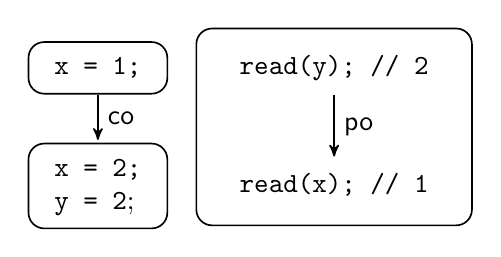
\begin{tikzpicture}[->,>=stealth',shorten >=1pt,auto,node distance=3cm,
    semithick, transform shape]
    \node[draw, rounded corners=2mm] (t1) at (0, 0) {\begin{tabular}{l} \texttt{x = 1;} \end{tabular}};
   \node[draw, rounded corners=2mm] (t2) at (0, -1.5) {\begin{tabular}{l} \texttt{x = 2;} \\ \texttt{y = 2};\end{tabular}};
   \node[draw, rounded corners=2mm, minimum width=3.5cm, minimum height=2.5cm] (t3) at (3, -0.75) {};
   \node (t3_1) at (3, 0) {\begin{tabular}{l} \texttt{read(y); // 2} \end{tabular}};
   \node (t3_2) at (3, -1.5) {\begin{tabular}{l} \texttt{read(x); // 1} \end{tabular}};
   % \path (t1) edge node {} (t3_2);
   % \path (t2) edge node {} (t3_1);
   \path (t1) edge node {$\co$} (t2);
   \path (t3_1) edge node {$\po$} (t3_2);
  \end{tikzpicture}  
    }
    \caption{$\mathsf{Read\ Committed}$ violation.}
    \label{rc_example:1}
    
\end{subfigure}
\begin{subfigure}{.32\textwidth}
\resizebox{\textwidth}{!}{
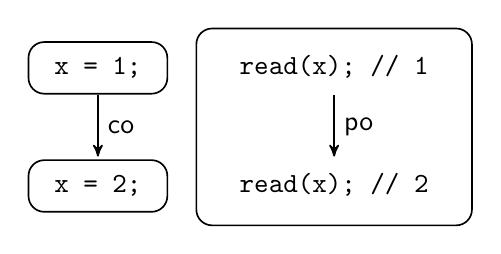
\begin{tikzpicture}[->,>=stealth',shorten >=1pt,auto,node distance=3cm,
 semithick, transform shape]
 \node[draw, rounded corners=2mm] (t1) at (0, 0) {\begin{tabular}{l} \texttt{x = 1;} \end{tabular}};
\node[draw, rounded corners=2mm] (t2) at (0, -1.5) {\begin{tabular}{l} \texttt{x = 2;} \end{tabular}};
\node[draw, rounded corners=2mm, minimum width=3.5cm, minimum height=2.5cm] (t3) at (3, -0.75) {};
\node (t3_1) at (3, -0) {\begin{tabular}{l} \texttt{read(x); // 1} \end{tabular}};
\node (t3_2) at (3, -1.5) {\begin{tabular}{l} \texttt{read(x); // 2} \end{tabular}};
% \path (t1) edge node {} (t3_1);
% \path (t2) edge node {} (t3_2);
\path (t1) edge node {$\co$} (t2);
\path (t3_1) edge node {$\po$} (t3_2);
\end{tikzpicture}  
}
 \caption{Repeatable Read violation.}
 \label{rr_example:1}
\end{subfigure}
\begin{subfigure}{.32\textwidth}
\resizebox{\textwidth}{!}{
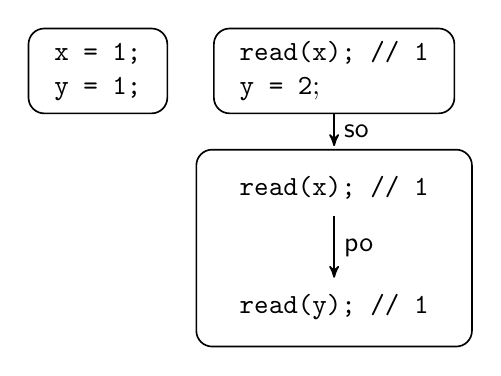
\begin{tikzpicture}[->,>=stealth',shorten >=1pt,auto,node distance=3cm,
 semithick, transform shape]
 \node[draw, rounded corners=2mm] (t1) at (0, 1.5) {\begin{tabular}{l} \texttt{x = 1;} \\ \texttt{y = 1;}\end{tabular}};
\node[draw, rounded corners=2mm] (t2) at (3, 1.5) {\begin{tabular}{l} \texttt{read(x); // 1} \\ \texttt{y = 2};\end{tabular}};
\node[draw, rounded corners=2mm, minimum width=3.5cm, minimum height=2.5cm] (t3) at (3, -0.75) {};
\node (t3_1) at (3, 0) {\begin{tabular}{l} \texttt{read(x); // 1} \end{tabular}};
\node (t3_2) at (3, -1.5) {\begin{tabular}{l} \texttt{read(y); // 1} \end{tabular}};
% \path (t1) edge node {} (t3);
\path (t2) edge node {$\so$} (t3);
% \path (t1) edge node {} (t2);
\path (t3_1) edge node {$\po$} (t3_2);
\end{tikzpicture}  
}
 \caption{Read My Writes violation.}
 \label{rmw_example:1}
\end{subfigure}
\begin{subfigure}{.32\textwidth}
\resizebox{\textwidth}{!}{
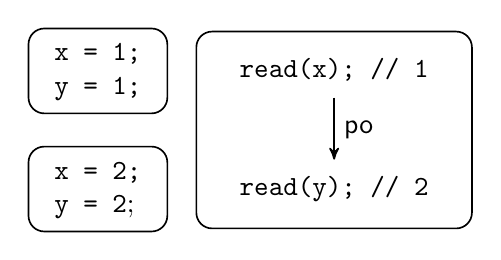
\begin{tikzpicture}[->,>=stealth',shorten >=1pt,auto,node distance=3cm,
 semithick, transform shape]
 \node[draw, rounded corners=2mm] (t1) at (0, 0) {\begin{tabular}{l} \texttt{x = 1;} \\ \texttt{y = 1;} \end{tabular}};
\node[draw, rounded corners=2mm] (t2) at (0, -1.5) {\begin{tabular}{l} \texttt{x = 2;} \\ \texttt{y = 2};\end{tabular}};
\node[draw, rounded corners=2mm, minimum width=3.5cm, minimum height=2.5cm] (t3) at (3, -0.75) {};
\node (t3_2) at (3, -1.5) {\begin{tabular}{l} \texttt{read(y); // 2} \end{tabular}};
\node (t3_1) at (3, -0) {\begin{tabular}{l} \texttt{read(x); // 1} \end{tabular}};
% \path (t1) edge node {} (t3_1);
% \path (t2) edge node {} (t3_2);
% \path (t1) edge node {$\co$} (t2);
\path (t3_1) edge node {$\po$} (t3_2);
\end{tikzpicture}  
}
 \caption{Repeatable Read violation.}
 \label{ra_example:1}
\end{subfigure}
\begin{subfigure}{.32\textwidth}
\resizebox{\textwidth}{!}{
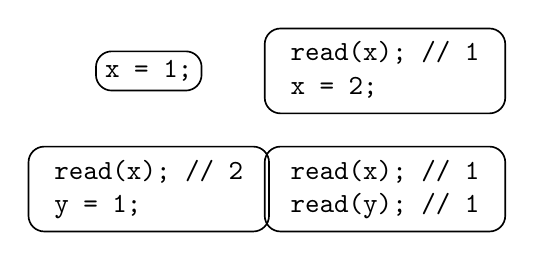
\begin{tikzpicture}[->,>=stealth',shorten >=1pt,auto,node distance=3cm,
 semithick, transform shape]
 \node[draw, rounded corners=2mm] (t1) at (0, 1.5) {\texttt{x = 1;}};
\node[draw, rounded corners=2mm] (t2) at (3, 1.5) {\begin{tabular}{l} \texttt{read(x); // 1} \\ \texttt{x = 2;} \end{tabular}};
\node[draw, rounded corners=2mm] (t3) at (3, 0) {\begin{tabular}{l} \texttt{read(x); // 1} \\ \texttt{read(y); // 1} \end{tabular}};
\node[draw, rounded corners=2mm] (t4) at (0, 0) {\begin{tabular}{l} \texttt{read(x); // 2} \\ \texttt{y = 1;} \end{tabular}};
% \path (t1) edge node {} (t3);
% \path (t2) edge node {$\so$} (t3);
% \path (t1) edge node {} (t2);
% \path (t3_1) edge node {$\po$} (t3_2);
\end{tikzpicture}  
}
 \caption{$\mathsf{Causal}$ violation.}
 \label{cc_example:1}
\end{subfigure}
\begin{subfigure}{.33\textwidth}
\resizebox{\textwidth}{!}{
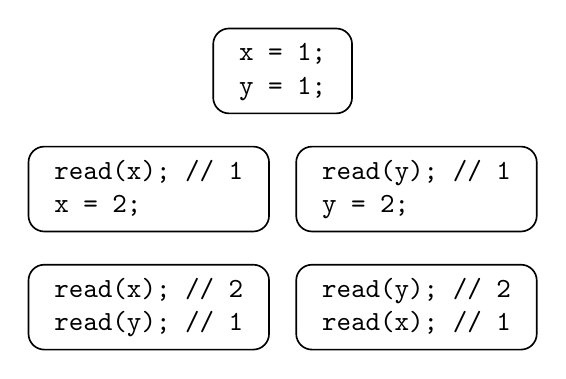
\begin{tikzpicture}[->,>=stealth',shorten >=1pt,auto,node distance=3cm,
 semithick, transform shape]
 \node[draw, rounded corners=2mm] (t1) at (0, 0) {\begin{tabular}{l} \texttt{x = 1;} \\ \texttt{y = 1;}\end{tabular}};
 \node[draw, rounded corners=2mm] (t2) at (-1.7, -1.5) {\begin{tabular}{l} \texttt{read(x); // 1} \\ \texttt{x = 2;} \end{tabular}};
\node[draw, rounded corners=2mm] (t3) at (1.7, -1.5) {\begin{tabular}{l} \texttt{read(y); // 1} \\ \texttt{y = 2;} \end{tabular}};
\node[draw, rounded corners=2mm] (t4) at (-1.7, -3) {\begin{tabular}{l} \texttt{read(x); // 2} \\ \texttt{read(y); // 1} \end{tabular}};
\node[draw, rounded corners=2mm] (t5) at (1.7, -3) {\begin{tabular}{l} \texttt{read(y); // 2} \\ \texttt{read(x); // 1} \end{tabular}};
% \node[draw, rounded corners=2mm] (t3) at (1.5, 0) {\begin{tabular}{l} \texttt{read(x); // 2} \\ \texttt{read(y); // 1} \end{tabular}};
% \path (t1) edge node {} (t3);
% \path (t2) edge node {$\so$} (t3);
% \path (t1) edge node {} (t2);
% \path (t3_1) edge node {$\po$} (t3_2);
\end{tikzpicture}  
}
 \caption{$\mathsf{Prefix}$ violation.}
 \label{pre_example:1}
\end{subfigure}
\begin{subfigure}{.32\textwidth}
\resizebox{\textwidth}{!}{
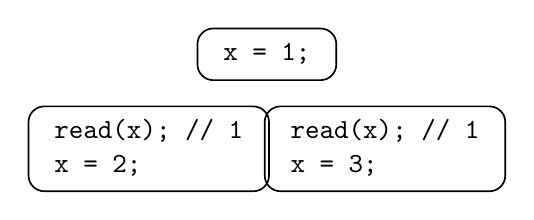
\begin{tikzpicture}[->,>=stealth',shorten >=1pt,auto,node distance=3cm,
 semithick, transform shape]
 \node[draw, rounded corners=2mm] (t1) at (0, 0) {\begin{tabular}{l} \texttt{x = 1;} \end{tabular}};
 \node[draw, rounded corners=2mm] (t2) at (-1.5, -1.2) {\begin{tabular}{l} \texttt{read(x); // 1} \\ \texttt{x = 2;} \end{tabular}};
 \node[draw, rounded corners=2mm] (t3) at (1.5, -1.2) {\begin{tabular}{l} \texttt{read(x); // 1} \\ \texttt{x = 3;} \end{tabular}};
 % \node[draw, rounded corners=2mm] (t3) at (0, -2.4) {\begin{tabular}{l} \texttt{read(x); // 2} \end{tabular}};
% \node[draw, rounded corners=2mm] (t3) at (1.7, -1.5) {\begin{tabular}{l} \texttt{read(y); // 1} \\ \texttt{y = 2;} \end{tabular}};
% \node[draw, rounded corners=2mm] (t3) at (1.5, 0) {\begin{tabular}{l} \texttt{read(x); // 2} \\ \texttt{read(y); // 1} \end{tabular}};
% \path (t1) edge node {} (t3);
% \path (t2) edge node {$\co$} (t3);
% \path (t1) edge node {} (t2);
% \path (t3_1) edge node {$\po$} (t3_2);
\end{tikzpicture} 
}
 \caption{$\mathsf{Conflict}$ violation.}
 \label{conf_example:1}
\end{subfigure}
\begin{subfigure}{.32\textwidth}
\resizebox{\textwidth}{!}{
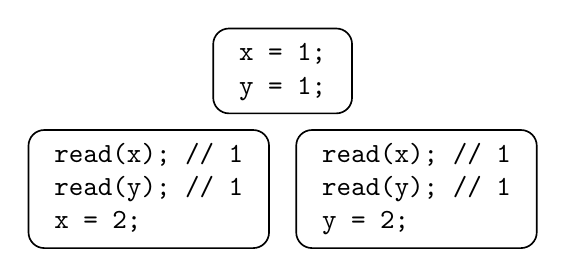
\begin{tikzpicture}[->,>=stealth',shorten >=1pt,auto,node distance=3cm,
 semithick, transform shape]
 \node[draw, rounded corners=2mm] (t1) at (0, 0) {\begin{tabular}{l} \texttt{x = 1;} \\ \texttt{y = 1;}\end{tabular}};
 \node[draw, rounded corners=2mm] (t2) at (-1.7, -1.5) {\begin{tabular}{l} \texttt{read(x); // 1} \\ \texttt{read(y); // 1} \\ \texttt{x = 2;} \end{tabular}};
 \node[draw, rounded corners=2mm] (t3) at (1.7, -1.5) {\begin{tabular}{l} \texttt{read(x); // 1} \\ \texttt{read(y); // 1} \\ \texttt{y = 2;} \end{tabular}};
% \node[draw, rounded corners=2mm] (t3) at (1.7, -1.5) {\begin{tabular}{l} \texttt{read(y); // 1} \\ \texttt{y = 2;} \end{tabular}};
% \node[draw, rounded corners=2mm] (t3) at (1.5, 0) {\begin{tabular}{l} \texttt{read(x); // 2} \\ \texttt{read(y); // 1} \end{tabular}};
% \path (t1) edge node {} (t3);
% \path (t2) edge node {$\so$} (t3);
% \path (t1) edge node {} (t2);
% \path (t3_1) edge node {$\po$} (t3_2);
\end{tikzpicture}  
}
 \caption{$\mathsf{Serializability}$ violation.}
 \label{ser_example:1}
\end{subfigure}

  \caption{Examples of histories used to explain the axioms in Figure~\ref{consistency_defs}. For readability, the $\wro$ relation is defined by the values written in comments with each {\tt read}.}
  \label{counter_example:1}
\vspace{-3mm}
\end{figure}

The axioms we use have a uniform shape: they define mandatory $\co$ predecessors $\tr_2$ of a transaction $\tr_1$ that is read in the history. For instance, the criterion called \textsc{Read Committed} (RC)~\cite{DBLP:conf/sigmod/BerensonBGMOO95} requires that every value read in the history was written by a committed transaction, and also, that the reads in the same transaction are ``monotonic'' in the sense that they do not return values that are older, w.r.t. the commit order, than other values read in the past\footnote{This monotonicity property corresponds to the fact that in the original formulation of \textsc{Read Committed}~\cite{DBLP:conf/sigmod/BerensonBGMOO95}, every write is guarded by the acquisition of a lock on the written variable, that is held until the end of the transaction.}. While the first condition holds for any history (because of the surjectivity of $\wro$), the second condition is expressed by the axiom $\mathsf{Read\ Committed}$ in Figure~\ref{lock_rc_def}. This axiom states that for any transaction $\tr_1$ writing a variable $\xvar$ that is read in a transaction $\tr$, the set of transactions $\tr_2$ writing $\xvar$ and read previously in the same transaction must precede $\tr_1$ in commit order. For instance, Figure~\ref{rc_example:1} shows a history and a (partial) commit order that does not satisfy this axiom because ${\tt read(x)}$ returns the value written in a transaction ``older'' than the transaction read in the previous ${\tt read(y)}$. An example of a history and commit order satisfying this axiom is given in Figure~\ref{rr_example:1}.

%TODO GIVE A POSITIVE AND A NEGATIVE EXAMPLE W.R.T. READ COMMITTED, AND EXPLAIN THE APPLICATION OF THIS AXIOM. THE EXAMPLES SHOULD BE "SYNTHETIC", WITH VARIABLES $\xvar$ and $\yvar$.
More precisely, the axioms are first-order formulas\footnote{These formulas are interpreted on tuples $\tup{\hist,\co}$ of a history $\hist$ and a commit order $\co$ on the transactions in $\hist$ as usual.} of the following form:
\begin{align}
  & \forall \xvar,\ \forall \tr_1,\tr_2,\ \forall \alpha.\ \tr_1\neq \tr_2\land \tup{\tr_1,\alpha}\in \wro[\xvar] \land \writeVar{\tr_2}{\xvar} \land \phi(\tr_2,\alpha) \implies \tup{\tr_2,\tr_1}\in\co \label{eq:axiom:cons}
\end{align}
where $\phi$ is a property relating $\tr_2$ and $\alpha$ (i.e., the read or the transaction reading from $\tr_1$) that varies from one axiom to another. Intuitively, this axiom schema states the following: in order for $\alpha$ to read specifically $t_1$'s write on $x$, it must be the case that every $t_2$ that also writes $x$ and satisfies $\phi(t_2,\alpha)$ was committed before $t_1$. Note that in all cases we consider, $\phi(t_2,\alpha)$ already ensures that $t_2$ is committed before the read $\alpha$, so this axiom schema ensures that $t_2$ is furthermore committed before $t_1$'s write.

The axioms used throughout the chapter are given in Figure~\ref{consistency_defs}. The property $\phi$ relates $\tr_2$ and $\alpha$ using the write-read relation and the session order in the history, and the commit order. 
%The axioms are first-order formulas whose satisfaction on tuples $\tup{\hist,\co}$ of a history $\hist$ and a commit order $\co$ on the transactions in $\hist$ is defined as usual.

In the following, we explain the rest of the consistency criteria we consider and the axioms defining them. \textsc{Read Atomic} (RA)~\cite{DBLP:conf/concur/Cerone0G15} is a strengthening of \textsc{Read Committed} defined by the axiom $\mathsf{Read\ Atomic}$, which states that for any transaction $\tr_1$ writing a variable $\xvar$ that is read in a transaction $\tr_3$, the set of $\wro$ or $\so$ predecessors of $\tr_3$ writing $\xvar$ must precede $\tr_1$ in commit order. The case of $\wro$ predecessors corresponds to the Repeatable Read criterion in~\cite{DBLP:conf/sigmod/BerensonBGMOO95}, which requires that successive reads of the same variable in the same transaction return the same value, Figure~\ref{rr_example:1} showing a violation, and also that every read of a variable $\xvar$ in a transaction $\tr$ returns the value written by the maximal transaction $\tr'$ (w.r.t. the commit order) that is read by $\tr$, Figure~\ref{ra_example:1} showing a violation (for any commit order between the transactions on the left, either ${\tt read(x)}$ or ${\tt read(y)}$ will return a value not written by the maximal transaction). The case of $\so$ predecessors corresponds to the  ``read-my-writes'' guarantee~\cite{DBLP:conf/pdis/TerryDPSTW94} concerning sessions, which states that a transaction $\tr$ must observe previous writes in the same session. For instance, {\tt read(y)} returning 1 in Figure~\ref{rmw_example:1} shows that the last transaction on the right does not satisfy this guarantee: the transaction writing 1 to {\tt y} was already visible to that session before it wrote 2 to {\tt y}, and therefore the value 2 should have been read. $\mathsf{Read\ Atomic}$ requires that the $\so$ predecessor of the transaction reading {\tt y} be ordered in $\co$ before the transaction writing 1 to {\tt y}, which makes the union $\co\cup\wro$ cyclic.

The following lemma shows that for histories satisfying $\mathsf{Read\ Atomic}$, the inverse of $\wro[\xvar]$ extended to transactions is a total function.

\begin{lemma}
 Let $\hist=\tup{T, \so, \wro}$ be a history. 
 If $\tup{\hist,\co}$ satisfies $\mathsf{Read\ Atomic}$, then %the extension of $\wro[\xvar]$ to transactions 
 for every transaction $\tr$ and two reads $\rd[\id_1]{\xvar}{\val_1},\rd[\id_2]{\xvar}{\val_2}\in \readOp{\tr}$, $\wro^{-1}(\rd[\id_1]{\xvar}{\val_1})=\wro^{-1}(\rd[\id_2]{\xvar}{\val_2})$ and $\val_1 = \val_2$.
\end{lemma}

\begin{proof}
  Let $\tup{\tr_1, \rd[\id_1]{\xvar}{\val_1}}, \tup{\tr_2, \rd[\id_2]{\xvar}{\val_2}} \in \wro[\xvar]$. Then $\tr_1, \tr_2$ write to $\xvar$. Let us assume by contradiction, that $\tr_1\neq\tr_2$. By \textsf{Read Atomic}, $\tup{\tr_2, \tr_1} \in \co$ because $\tup{\tr_1, \rd[\id_1]{\xvar}{\val_1}} \in \wro[\xvar]$ and $\tr_2$ writes to $\xvar$. Similarly, we can also show that $\tup{\tr_1, \tr_2} \in \co$. This contradicts the fact that $\co$ is a strict total order. Therefore, $\tr_1 = \tr_2$. We also have that $\val_1 = \val_2$ because each transaction contains a single write to $\xvar$.
\end{proof}

\textsc{Causal Consistency} (CC)~\cite{DBLP:journals/cacm/Lamport78} is defined by the axiom $\mathsf{Causal}$, which states that for any transaction $\tr_1$ writing a variable $\xvar$ that is read in a transaction $\tr_3$, the set of $(\wro\cup \so)^+$ predecessors of $\tr_3$ writing $\xvar$ must precede $\tr_1$ in commit order ($(\wro\cup \so)^+$ is usually called the \emph{causal} order). A violation of this axiom can be found in Figure~\ref{cc_example:1}: the transaction $\tr_2$ writing 2 to {\tt x} is a $(\wro\cup \so)^+$ predecessor of the transaction $\tr_3$ reading 1 from {\tt x} because the transaction $\tr_4$, writing 1 to {\tt y}, reads {\tt x} from $\tr_2$ and $\tr_3$ reads {\tt y} from $\tr_4$. This implies that $\tr_2$ should precede in commit order the transaction $\tr_1$ writing 1 to {\tt x}, which again, is inconsistent with the write-read relation ($\tr_2$ reads from $\tr_1$).

\begin{table}[t]
 \caption{Consistency model definitions}
%  \vspace{2mm}
 \centering
 % \resizebox{\textwidth}{!}{
 \begin{tabular}{|l|l|}
  \hline
  \shortstack{Consistency model}   & Axioms                                   \\
  \hline
  \textsc{Read Committed} (RC)     & $\mathsf{Read\ Committed}$               \\
  \hline
  \textsc{Read Atomic} (RA)        & $\mathsf{Read\ Atomic}$                  \\
  \hline
  \textsc{Causal consistency} (CC) & $\mathsf{Causal}$                        \\
  \hline
  \textsc{Prefix consistency} (PC) & $\mathsf{Prefix}$                        \\
  \hline
  \textsc{Snapshot isolation} (SI) & $\mathsf{Prefix}\land \mathsf{Conflict}$ \\
  \hline
  \textsc{Serializability} (SER)   & $\mathsf{Serializability}$               \\
  \hline
  % \multicolumn{3}{|c|}{
  %  $\textbf{RA} \supset \textbf{CC} \supset \textbf{PC} \supset \textbf{SI} \supset \textbf{SER}$
  % }                                                                   \\
  % \hline
 \end{tabular}
 % }
 \label{weakconsistency:2}
% \vspace{-5mm}
\end{table}

\textsc{Prefix consistency} (PC)~\cite{DBLP:conf/ecoop/BurckhardtLPF15} is a strengthening of CC, which requires that every transaction observes a prefix of a commit order between all the transactions. With the intuition that the observed transactions are $\wro\cup\so$ predecessors, the axiom $\mathsf{Prefix}$ defining PC, states that for any transaction $\tr_1$ writing a variable $\xvar$ that is read in a transaction $\tr_3$, the set of $\co^*$ predecessors of transactions observed by $\tr_3$ writing $\xvar$ must precede $\tr_1$ in commit order (we use $\co^*$ to say that even the transactions observed by $\tr_3$ must precede $\tr_1$). This ensures the prefix property stated above. An example of a PC violation can be found in Figure~\ref{pre_example:1}: the two transactions on the bottom read from the three transactions on the top, but any serialization of those three transactions will imply that one of the combinations {\tt x=1}, {\tt y=2} or {\tt x=2}, {\tt y=1} cannot be produced at the end of a prefix in this serialization.

\textsc{Snapshot Isolation} (SI)~\cite{DBLP:conf/sigmod/BerensonBGMOO95} is a strengthening of PC that disallows two transactions to observe the same prefix of a commit order if they \emph{conflict}, i.e., write to a common variable. It is defined by the conjunction of $\mathsf{Prefix}$ and another axiom called $\mathsf{Conflict}$, which requires that for any transaction $\tr_1$ writing a variable $\xvar$ that is read in a transaction $\tr_3$, the set of $\co^*$ predecessors writing $\xvar$ of transactions conflicting with $\tr_3$ and before $\tr_3$ in commit order, must precede $\tr_1$ in commit order. Figure~\ref{conf_example:1} shows a $\mathsf{Conflict}$ violation.

Finally, \textsc{Serializability} (SER)~\cite{DBLP:journals/jacm/Papadimitriou79b} is defined by the axiom with the same name, which requires that for any transaction $\tr_1$ writing to a variable $\xvar$ that is read in a transaction $\tr_3$, the set of $\co$ predecessors of $\tr_3$ writing $\xvar$ must precede $\tr_1$ in commit order. This ensures that each transaction observes the effects of all the $\co$ predecessors. Figure~\ref{ser_example:1} shows a $\mathsf{Serializability}$ violation.

The next lemma states the relationship between these axioms.

\begin{lemma}
 The following entailments hold:
 \begin{align*}
   & \mathsf{Causal} \implies \mathsf{Read\ Atomic}\implies \mathsf{Read\ Committed} \\
   & \mathsf{Prefix} \implies \mathsf{Causal}                                        \\
   & \mathsf{Serializability} \implies \mathsf{Prefix}\land \mathsf{Conflict}        
 \end{align*} 
 \label{axioms-rel}
\end{lemma}

\begin{proof}
  We will show the contrapositive of each implication:
 \begin{itemize}
   \item If $\tup{\hist, \co}$ does not satisfy \textsf{Read Committed},  then
\begin{align*}
\exists \xvar,\ \exists \tr_1,\tr_2,\ \exists \alpha,\beta.\ \tup{\tr_1,\alpha}\in \wro[\xvar] \land \writeVar{\tr_2}{\xvar}\ \land \tup{\tr_2,\beta}\in\wro \land \tup{\beta,\alpha} \in \po \land \tup{\tr_1,\tr_2}\in\co. 
\end{align*}
Let $\tr_3$ the transaction containing $\alpha$ and $\beta$. We have that $\tup{\tr_2, \tr_3} \in \wro$. But then we have $\tr_1, \tr_2, \tr_3$ such that $\tup{\tr_1, \tr_3} \in \wro[\xvar]$ and $\tup{\tr_2, \tr_3} \in \wro$ and $\writeVar{\tr_2}{\xvar}$. So by \textsf{Read Atomic}, $\tup{\tr_2, \tr_1} \in \co$. This contradicts the fact that $\co$ is a strict total order. Therefore, $\tup{\hist, \co}$ does not satisfy \textsf{Read\ Atomic}.
   \item If $\tup{\hist, \co}$ does not satisfy \textsf{Read Atomic}, then 
 \begin{align*}  
 \exists \xvar, \exists \tr_1,\tr_2,\tr_3.\ \tup{\tr_1,\tr_3}\in \wro[\xvar] \land \writeVar{\tr_2}{\xvar}\ \land \tup{\tr_2,\tr_3}\in\wro\cup\so \land \tup{\tr_1,\tr_2}\in\co.
 \end{align*}
  Then $\tup{\tr_2,\tr_3}\in(\wro\cup\so)^+$. Then, by \textsf{Causal}, we have $\tup{\tr_2, \tr_1} \in \co$, which contradicts the fact that $\co$ is a strict total order. Therefore, $\tup{\hist, \co}$ does not satisfy \textsf{Causal}.
   \item If $\tup{\hist, \co}$ does not satisfy \textsf{Causal}, then
\begin{align*}
\exists \xvar, \exists \tr_1,\tr_2,\tr_3.\ \tup{\tr_1,\tr_3}\in \wro[\xvar] \land \writeVar{\tr_2}{\xvar}\ \land \tup{\tr_2,\tr_3}\in(\wro\cup\so)^+ \land\tup{\tr_1,\tr_2}\in\co.
\end{align*}
   But, $(\wro\cup\so)^+ = (\wro\cup\so)^* \circ (\wro\cup\so) \subseteq \co^* \circ (\wro\cup\so)$. Therefore, $\tup{\tr_2,\tr_3}\in\co^* \circ (\wro\cup\so)$. Then, by \textsf{Prefix}, we have $\tup{\tr_2, \tr_1} \in \co$, which contradicts the fact that $\co$ is a strict total order. Therefore, $\tup{\hist, \co}$ does not satisfy \textsf{Prefix}.
   \item If $\tup{\hist, \co}$ does not satisfy \textsf{Prefix} or \textsf{Conflict}, then 
\begin{align*}
\exists \xvar, \exists \tr_1,\tr_2,\tr_3, \tr_4.\ \tup{\tr_1,\tr_3}\in \wro[\xvar] \land \writeVar{\tr_2}{\xvar}\ \land \tup{\tr_2,\tr_4}\in\co^* \land \tup{\tr_1,\tr_2}\in\co
\end{align*}
and 
       \begin{itemize}
         \item $\tup{\tr_4,\tr_3}\in \co \land \writeVar{\tr_3}{\yvar}\ \land \writeVar{\tr_3}{\yvar}$ if it violates \textsf{Conflict}.
         \item $\tup{\tr_4,\tr_3}\in (\wro \cup \so)$ if it violates \textsf{Prefix}.
       \end{itemize}
       
In both cases, we have that $\tup{\tr_4, \tr_3} \in \co$. Because $\co$ is transitive, $\tup{\tr_2, \tr_4} \in \co^*$ and $\tup{\tr_4, \tr_3} \in \co$ imply that $\tup{\tr_2, \tr_3} \in \co$. Then by \textsf{Serializability}, we have $\tup{\tr_2, \tr_1} \in \co$, which contradicts the fact that $\co$ is a strict total order. Therefore, $\tup{\hist, \co}$ does not satisfy \textsf{Serializability}.
 \end{itemize}
\end{proof}


\begin{definition}
 Given a set of axioms $X$ defining a criterion $C$ like in Table~\ref{weakconsistency:2}, a history $\hist=\tup{T, \so, \wro}$ \emph{satisfies} $C$ iff there exists a strict total order $\co$ such that $\wro\cup\so\subseteq \co$ and $\tup{h,\co}$ satisfies $X$.
 % Given a $\CO$(\textit{commit order}), a total order on $T$ which extends $\wro \cup \so$, we can define consistency axioms from table \ref{consistency_defs}. For each axiom, the situation in the table implies, $\Path{\tr_2}{\CO}{\tr_1}$.
 \label{axiom-criterion}
\end{definition}

Definition~\ref{axiom-criterion} and Lemma~\ref{axioms-rel} imply that each consistency criterion in Table~\ref{weakconsistency:2} is stronger than its predecessors (reading them from top to bottom), e.g., CC is stronger than RA and RC. This relation is known to be strict~\cite{DBLP:conf/concur/Cerone0G15}, e.g., RA is not stronger than CC. 
%stronger from top to bottom order. Infact each criteria is strictly stronger than its previously weaker criteria, \ie \textsf{Snapshot Isolation} does not imply \textsf{Serializability}. 
 % (see Appendix~\ref{app:gotsman}).

%\begin{table}
% \begin{tabular}{|c|c|}
%  \hline
%  Axioms          & Anomaly                                  \\
%  \hline
%  Causal          & Causal violation                         \\
%  \hline
%  Prefix          & Causal violation, Long fork              \\
%  \hline
%  Conflict        & Lost update                              \\
%  \hline
%  Serializability & \shortstack{Causal violation, Long fork, \\ Lost update, Write Skew}\\
%  \hline 
% \end{tabular}
% \caption{Axioms and anomalies}
% \label{axiom_anomaly}
%\end{table}

%\begin{definition}
% We define consistency criteria using the definitions in table \ref{weakconsistency:2}.
%\end{definition}



% For simplicity, in all the following definitions, when we say, there exists a $\CO$\textit{(commit order)}, we will implicitly mean, $\CO$ is a total order on $T$ which extends $\WR \cup \SO$.
% 
% \begin{definition}
%  By our definition of history, history is Read committed.
% \end{definition}
% 
% 
% \begin{definition}
%  A history is Locking Read Committed, if there exists a $\CO$, such that for any variables $x,y$ and transactions $\tr_1$, $\tr_2$ and two operations $\op_1$, $\op_2$ in any situation illustrated in figure \ref{lock_rc_def}, $\Path{\tr_2}{\CO}{\tr_1}$ always.
% \end{definition}
% 
% \begin{definition}
%  A history is Read atomic, resp., Causal consistency, Prefix consistency, Conflict consistency, Serializability, if there exists a $\CO$, such that for any variable $\xvar$ and transactions $\tr_1$, $\tr_2$, $\tr_3$ in the resp. situations illustrated in figure \ref{consistency_defs}, $\Path{\tr_2}{\CO}{\tr_1}$ always.
% \end{definition}

% \begin{definition}
%  The sets of histories and schedules allowed by a particular weak model - `wm' can be defined as:
% \end{definition}
% 
% \begin{itemize}
%  \item $\textsf{Sche}_{wm} = \left\{ \mathcal{S} \mid S \models \text{axioms of } wm \right\}$
%  \item $\textsf{Hist}_{wm} = \left\{ \mathcal{H} \mid \exists \VIS, \CO, (\mathcal{H}, VIS, CO)\right\}$
% \end{itemize}
% 
% So to verify a history for a consistency model, it suffices to find a schedule, in particular, \VIS, \CO for that history, which satisfies the axioms for that consistency model.


% \begin{table*}
%  \centering
%  \resizebox{\textwidth}{!}{
%   \begin{tabular}{|c|l|l|c|c|c|c|c|}
%    \hline
%    $\Phi$       & \shortstack{Consistency model                                                                                                                            \\ (strong session)} & Axioms & \shortstack{Fractured \\ reads} & \shortstack{Causality \\ violation} & \shortstack{Lost \\ update} & \shortstack{Long \\ fork} & \shortstack{Write \\ skew} \\
%    \hline
%    \textbf{RA}  & Read atomic                   & \textsc{Int} $\wedge$ \textsc{Ext} $\wedge$ \textsc{Session} & \ding{55} & \ding{51} & \ding{51} & \ding{51} & \ding{51} \\
%    \hline
%    \textbf{CC}  & Causal consistency            & \textbf{RA} $\wedge$ \textsc{TransVis}                       & \ding{55} & \ding{55} & \ding{51} & \ding{51} & \ding{51} \\
%    \hline
%    \textbf{PC}  & Prefix consistency            & \textbf{RA} $\wedge$  \textsc{Prefix}                        & \ding{55} & \ding{55} & \ding{51} & \ding{55} & \ding{51} \\
%    \hline
%    \textbf{SI}  & Snapshot isolation            & \textbf{PC} $\wedge$ \textsc{NoConflict}                     & \ding{55} & \ding{55} & \ding{55} & \ding{55} & \ding{51} \\
%    \hline
%    \textbf{SER} & Serializability               & \textbf{RA} $\wedge$ \textsc{TotalVis}                       & \ding{55} & \ding{55} & \ding{55} & \ding{55} & \ding{55} \\
%    \hline
%    \multicolumn{8}{|c|}{
%     $\textbf{RA} \supset \textbf{CC} \supset \textbf{PC} \supset \textbf{SI} \supset \textbf{SER}$
%    }                                                                                                                                                                       \\
%    \hline
%   \end{tabular}
%  }
%  \caption{Consistency model definitions, anomalies and relationship}
%  \label{weakconsistency:2}
% \end{table*}


%$T \xrightarrow{\VIS} S$ means all the writes of $T$ are visible to $S$. $T \xrightarrow{\CO} S$ means all the writes of $T$ are committed before $S$ committed all its writes. $\VIS \subseteq \CO$ ensures a transaction $T$ can be visible to another transaction $S$, if only $T$ is committed before $S$.

  % \input{Sources/transaction/sec3-temp}
  %!TEX root = Thesis.tex

% \section{Algorithms}
% 
% \subsection{Dependency Graph}
% 
% To formally reason about these consistencies over a history, we represent transactions as vertices in a graph and the relation dependencies using edges.
% 
% \begin{definition}
%  A tuple $\mathcal{G} = (\mathcal{T}, \SO, \WR, \WW, \RW)$ is a \textbf{dependency graph} for a history $\mathcal{H} = (\mathcal{T}, \SO, \WR)$, where
% \end{definition}
% 
% \begin{itemize}
%  \item $\SO$ is just session order of the history.
%  \item $\WR = \left\{ \WR_x \mid \text{x is a variable}\right\}$ where $T \xrightarrow{\WR_x} S \Leftrightarrow \exists n. T \models \texttt{write}(x, n) \land S \models \texttt{read}(x, n)$
%  \item $\WW = \left\{ \WW_x \mid \text{x is a variable}\right\}$ where $\WW_x$ is a total order on the set $\textsf{Write}_x$.
%  \item $\RW = \left\{ \RW_x \mid \text{x is a variable}\right\}$ where $T \xrightarrow{\RW_x} S \Leftrightarrow T \models \texttt{read}(x, \_) \land (\exists T'. T' \xrightarrow{\WR_x} T \Rightarrow T'\xrightarrow{\WW_x} S)$
% \end{itemize}
% 
% But not all such edge combinations are valid for a consistent schedule. For a Read Atomic consistent schedule, the edge dependencies must satisfy some properties.
% 
% \begin{definition}
%  \label{dependency}
%  Given a \textbf{schedule}, we can extract different type of dependencies between each transaction.
% \end{definition}
% 
% \begin{itemize}
%  \item \textbf{\textit{session dependency}} $T \xrightarrow{\SO} S \Leftrightarrow$ $T$, $S$ are in same session and $T$ happens before $S$.
%  \item \textbf{\textit{write-read dependency}} $T \xrightarrow{\WR_x} S \Leftrightarrow S \models \texttt{read}(x, \_) \land T = max_{\CO}(\VIS^{-1}(S) \cap \textsf{Write}_x)$
%  \item \textbf{\textit{write-write dependency}} $T \xrightarrow{\WW_x} S \Leftrightarrow T, S \in \textsf{Write}_x \land T \xrightarrow{\CO} S$
%  \item \textbf{\textit{read-write dependency}} $T \xrightarrow{\RW_x} S \Leftrightarrow T \models \texttt{read}(x, \_) \land (\exists T'. T' \xrightarrow{\WR_x} T \Rightarrow T'\xrightarrow{\WW_x} S)$
% \end{itemize}
% 
% \begin{corollary}
%  For any Read Atomic schedule $\mathcal{S}$, $graph(\mathcal{S}) = (\mathcal{T}_{\mathcal{S}}, \SO_{\mathcal{S}}, \WR_{\mathcal{S}}, \WW_{\mathcal{S}}, \RW_{\mathcal{S}})$ is a dependency graph for $\mathcal{H}_{\mathcal{S}}$.
% \end{corollary}
% 
% 
% % Now we have a characterization of weak consistent models using these dependencies. So verifying a history for a consistency model, becomes a problem for finding appropriate dependencies between the transactions, rather than visibility and commit order. To do that, we will extend these dependencies to \emph{dependency graphs} which includes edges representing the dependencies.
% 
% Intuitively, we can now represent the problem of finding a $wm$-consistent schedule using the problem of finding a dependency graph which satisfies such properties. Using this characterization for \textsc{Ext}, we have more stronger properties for each consistency criteria \cite{gotsmanpodc16, gotsmanconcur16}.
% 
% \begin{lemma}
%  If a schedule $\mathcal{S}$ satisfies $wm$-consistency, $graph(\mathcal{S})$ satisfies following properties.
% \end{lemma}
% 
% \begin{itemize}
%  \item \textbf{Causal consistency}: All cycles in $graph(\mathcal{S})$ must have at least one \RW edge and one another \RW or \WW edge.
%  \item \textbf{Prefix consistency}: All cycles in $graph(\mathcal{S})$ must have at least one $\RW$ edge with either a preceding $\WW$ edges or an another preceding $\RW$ edge.
%  \item \textbf{Snapshot isolation}: All cycles in $graph(\mathcal{S})$ must have at least two adjacent $\RW$ edges.
%  \item \textbf{Serialization}: $graph(\mathcal{S})$ has no cycle.
% \end{itemize}
% 
% 
% 
% To explain the cycles,
% 
% \begin{itemize}
%  \item First note, there should not be any cycle of the form $T \xrightarrow{\VIS} S \xrightarrow{\RW_x} T$. Because, then $\exists T', T' \xrightarrow{\WW_x} T, T' \xrightarrow{\WR_x} S$ and $T' = max_{\CO}(\VIS^{-1}(S) \cap \textsf{Write}_x)$. Since $T \in \VIS^{-1}(S)$, then we will have $T \xrightarrow{\CO} T' \xrightarrow{\WW_x} T$ which is not possible.
%  \item Also $\SO \cup \WR \subseteq \VIS$ and $\SO \cup \WR \cup \WW \subseteq \CO$.
%  \item To break the cycles in \CO, each cycle must have one dependency edge from \RW. But in causal consistency \SO and \WR must be included in \VIS and it must be transitive. So $(\SO \cup \WR)^+ ; \RW$ can not be cyclic. So, we need another \RW or \WW dependency edge.
%  \item Prefix consistency says, $\CO; \VIS \subseteq \VIS$ which imposes, $\VIS; \RW \subseteq \CO$. Which means, to break the cycles in \CO, extra \RW or \WW edge must precede \RW edge in all cycles.
%  \item Snapshot isolation says, $\WW_x \subseteq \VIS$ so $\WW_x$ can not break paths in \VIS anymore. So \RW edge must precede another \RW edges in all cycles.
%  \item Serialization says $\VIS = \CO$. So if $T \xrightarrow{\RW_x} S$ and $S \xrightarrow{\CO} T$ then, $S \xrightarrow{\VIS} T \xrightarrow{\RW_x} S$ which is not allowed. So $T \xrightarrow{\RW_x} S \Rightarrow T \xrightarrow{\VIS} S$ or $\RW \subseteq \VIS = \CO$. Hence $(\SO \cup \WR \cup \WW \cup \RW) \subseteq \CO = \VIS$.
% \end{itemize}
% 
% 
% 
% Now we say, this properties are are also enough for a dependency graph of a history to find respective $wm$-consistent schedule. In table \ref{depgraphcovis:1}, we have defined \CO and \VIS for $wm$-consistencies in terms of \SO, \WR, \WW, \RW.
% 
% \begin{lemma}
%  If a dependency graph $\mathcal{G}$ of a history $\mathcal{H}$, satisfies following properties, it is also $wm$-consistent.
% \end{lemma}
% 
% \begin{itemize}
%  \item $\mathcal{H}$ is \textbf{Causal consistent}, if all cycles in $\mathcal{G}$ must have at least one \RW edge and one another \RW or \WW edge, then
%  \item $\mathcal{H}$ is \textbf{Prefix consistent}, if all cycles in $\mathcal{G}$ must have at least one $\RW$ edge with either a preceding $\WW$ edges or an another preceding $\RW$ edge, then $\mathcal{H}$ is Serializable.
%  \item $\mathcal{H}$ is \textbf{Snapshot isolation}, if all cycles in $\mathcal{G}$ must have at least two adjacent $\RW$ edges, then $\mathcal{H}$ is Serializable.
%  \item $\mathcal{H}$ is \textbf{Serializable}, if $\mathcal{G}$ has no cycle.
% \end{itemize}
% 
% \begin{table*}
%  \centering
%  \resizebox{\textwidth}{!}{
%   \begin{tabular}{|c|c|c|}
%    \hline
%    Consistency model  & \CO                                                                    & \VIS                                                        \\
%    \hline
%    Causal consistency & $(\SO \cup \WR \cup \WW)^{total}$                                      & $(\SO \cup \WR)^+$                                          \\
%    \hline
%    Prefix consistency & $((\SO \cup \WR \cup \WW) \cup ((\SO \cup \WR);\RW))^{total}$          & $(\SO \cup \WR) \cup (\CO;(\SO \cup \WR))$                  \\
%    \hline
%    Snapshot isolation & $((\SO \cup \WR \cup \WW) \cup ((\SO \cup \WR \cup \WW);\RW))^{total}$ & $(\SO \cup \WR\cup \WW) \cup (\CO;(\SO \cup \WR \cup \WW))$ \\
%    \hline
%    Serialization      & $(\SO \cup \WR \cup \WW \cup \RW)^{total}$                             & \CO                                                         \\
%    \hline
%   \end{tabular}
%  }
%  \caption{\CO and \VIS relation from dependency graph}
%  \label{depgraphcovis:1}
% \end{table*}
% 
% \begin{proof}
%  We will show the \CO, \VIS relations from table. \ref{depgraphcovis:1} satisfies the axioms of respective consistencies.
%  \begin{itemize}
%   \item \CO is total. We will just show underlying graph is acyclic. \CO is just any total order on that acyclic graph.
%         \begin{itemize}
%          \item Causal consistency. Any cycle in $(\SO \cup \WR \cup \WW)$ would imply a cycle without any \RW edge.
%          \item Prefix consistency.
%                \begin{itemize}
%                 \item Any cycle in $(\SO \cup \WR \cup \WW)$ would imply cycle without any \RW edge.
%                 \item Any cycle in $((\SO \cup \WR);\RW)$ or $((\SO \cup \WR \cup \WW) \cup ((\SO \cup \WR);\RW))$ would a cycle with all \RW edges preceded by \SO or \WR edge.
%                \end{itemize}
%          \item Snapshot isolation.
%                \begin{itemize}
%                 \item Any cycle in $(\SO \cup \WR \cup \WW)$ would imply cycle without any \RW edge.
%                 \item Any cycle in $((\SO \cup \WR \cup \WW);\RW)$ or $((\SO \cup \WR \cup \WW) \cup ((\SO \cup \WR \cup \WW);\RW))$ would imply a cycle with all \RW edges preceded by \SO or \WR or \WW edge.
%                \end{itemize}
%          \item Serialization. $(\SO \cup \WR \cup \WW \cup \RW)$ does not have any cycle.
%         \end{itemize}
%   \item $\VIS \subseteq \CO$.
%         \begin{itemize}
%          \item Causal consistency. $(\SO \cup \WR) \subseteq \CO$. Then, also $(\SO \cup \WR)^+ \subseteq \CO^+ = \CO$.
%          \item Prefix consistency. $(\SO \cup \WR) \subseteq \CO$. Then, also $(\CO; (\SO \cup \WR)) \subseteq (\CO;\CO) = \CO$.
%          \item Snapshot isolation. $(\SO \cup \WR \cup \WW) \subseteq \CO$. Then, also $(\CO; (\SO \cup \WR \cup \WW)) \subseteq (\CO;\CO) = \CO$.
%          \item Serialization. $\VIS = \CO$
%         \end{itemize}
%   \item Read atomic:
%         \begin{itemize}
%          \item \session. $\SO \subseteq \VIS$.
%          \item \ext. $\VIS; \RW$ is acyclic.
%                \begin{itemize}
%                 \item Causal consistency. A cycle in $\VIS; \RW = (\SO \cup \WR)^+; \RW$ would imply a cycle with single \RW edge and no \WW edge.
%                 \item Prefix consistency. A cycle in $\VIS; \RW$ implies either cycle in $(\SO \cup \WR); \RW$ or $(\CO; (\SO \cup \WR); \RW)$.
%                       \begin{itemize}
%                        \item A cycle in $(\SO \cup \WR); \RW$ would imply a cycle with single \RW edge and no \WW edge.
%                        \item A cycle in $(\CO; (\SO \cup \WR); \RW)$ would imply $T_1 \xrightarrow{\CO} T_2 \xrightarrow{\SO \cup \WR} T_3 \xrightarrow{\RW} T_1$. But $((\SO \cup \WR); \RW) \subseteq \CO$. So $T_1 \xrightarrow{\CO} T_2 \xrightarrow{\CO} T_1$. But \CO is acylic.
%                       \end{itemize}
%                 \item Snapshot isolation. A cycle in $\VIS; \RW$ implies either cycle in $(\SO \cup \WR \cup \WW); \RW$ or $(\CO; (\SO \cup \WR \cup \WW); \RW)$.
%                       \begin{itemize}
%                        \item A cycle in $(\SO \cup \WR \cup \WW); \RW$ would imply a cycle with single \RW edge.
%                        \item A cycle in $(\CO; (\SO \cup \WR \cup \WW); \RW)$ would imply $T_1 \xrightarrow{\CO} T_2 \xrightarrow{\SO \cup \WR \cup \WW} T_3 \xrightarrow{\RW} T_1$. But $((\SO \cup \WR \cup \WW); \RW) \subseteq \CO$. So $T_1 \xrightarrow{\CO} T_2 \xrightarrow{\CO} T_1$. But \CO is acylic.
%                       \end{itemize}
%                 \item Serialization. $\RW \subseteq \VIS$ and \VIS is acyclic.
%                \end{itemize}
%         \end{itemize}
%   \item Satisfies respective axioms for other consistencies.
%         \begin{itemize}
%          \item Causal consistency.
%                \begin{itemize}
%                 \item \textsc{TransVis}. $\VIS$ is transitive by construction.
%                \end{itemize}
%          \item Prefix consistency.
%                \begin{itemize}
%                 \item \textsc{Prefix}.
%                       \begin{equation*}
%                        \begin{split}
%                         \CO; \VIS &= \CO; ((\SO \cup \WR) \cup (\CO;(\SO \cup \WR))) \\
%                         &= (\CO;(\SO \cup \WR)) \cup (\CO;\CO;(\SO \cup \WR)) \\
%                         &= (\CO;(\SO \cup \WR)) \\
%                         &= \VIS\\
%                        \end{split}
%                       \end{equation*}
%                \end{itemize}
%          \item Snapshot isolation.
%                \begin{itemize}
%                 \item \prefix.
%                       \begin{equation*}
%                        \begin{split}
%                         \CO; \VIS &= \CO; ((\SO \cup \WR \cup \WW) \cup (\CO;(\SO \cup \WR \cup \WW))) \\
%                         &= (\CO;(\SO \cup \WR \cup \WW)) \cup (\CO;\CO;(\SO \cup \WR \cup \WW)) \\
%                         &= (\CO;(\SO \cup \WR \cup \WW)) \\
%                         &= \VIS\\
%                        \end{split}
%                       \end{equation*}
%                \end{itemize}
%                \begin{itemize}
%                 \item \noconflict. $\WW \subseteq \VIS$
%                \end{itemize}
%          \item Serialization. $\VIS = \CO$.
%         \end{itemize}
%  \end{itemize}
% \end{proof}
% 
% Now, we can define,
% $$\textsf{DepGraph}_{wm} = \left\{\mathcal{G} = (\mathcal{T}, \SO, \WR, \WW, \RW) | \text{all cycles in } \mathcal{G} \text{ are allowed in $wm$-consistency}\right\}$$
% 
% Then we have,
% \begin{itemize}
%  \item $\forall \mathcal{S} \in \textsf{Sche}_{wm}. graph(\mathcal{S}) \in \textsf{DepGraph}_{wm}$
%  \item $\forall \mathcal{G} \in \textsf{DepGraph}_{wm}. \exists \mathcal{S} \in \textsf{Sche}_{wm}. graph(\mathcal{S}) = \mathcal{G}$
% \end{itemize}

\section{Checking Consistency Criteria}\label{sec:general}

% So we have reduced the problem of verifying a history to the problem of finding appropriate dependencies between transactions of dependency edges in a dependency graph which satisfies the semantic definition of a consistency.

This section establishes the complexity of checking the different consistency criteria in Table~\ref{weakconsistency:2} for a given history. More precisely, we show that \textsc{Read Committed}, \textsc{Read Atomic}, and \textsc{Causal Consistency} can be checked in polynomial time while the problem of checking the rest of the criteria is NP-complete. 

\begin{figure}
% \begin{subfigure}{.22\textwidth}
%  \resizebox{\textwidth}{!}{
%   \begin{tikzpicture}[->,>=stealth',shorten >=1pt,auto,node distance=3cm,
%     semithick, transform shape]
%    \node[draw, rounded corners=2mm] (t1) at (0, .2) {\begin{tabular}{l} \texttt{x = 1;} \\ \texttt{y = 1;} \end{tabular}};
%    \node[draw, rounded corners=2mm] (t2) at (0, -1.7) {\begin{tabular}{l} \texttt{x = 2;} \\ \texttt{y = 2;} \end{tabular}};
%    \node[draw, rounded corners=2mm, minimum width=3.5cm, minimum height=3.2cm] (t3) at (3, -0.7) {};
%    \node[draw=black!50, rounded corners=2mm, dashed] (t3_1) at (3, .4) {\begin{tabular}{l} \texttt{read(x); // 1} \end{tabular}};
%    \node[draw=black!50, rounded corners=2mm, dashed] (t3_2) at (3, -.7) {\begin{tabular}{l} \texttt{read(y); // 2} \end{tabular}};
%    \node[draw=black!50, rounded corners=2mm, dashed] (t3_3) at (3, -1.8) {\begin{tabular}{l} \texttt{read(x); // 1} \end{tabular}};
%    \path (t3_1) edge[red] node {$\po$} (t3_2);
%    \path (t1) edge[red, bend left] node {$\co$} (t2);
%    \path (t3_2) edge[blue] node {$\po$} (t3_3);
%    \path (t2) edge[blue, bend left] node {$\co$} (t1);
%   \end{tikzpicture}  
%  }
%  \caption{\emph{not} Read committed}
%  \label{rc_algo_counter_example:1}
% \end{subfigure}
% 
% \begin{subfigure}{.22\textwidth}
%  \resizebox{\textwidth}{!}{
%   \begin{tikzpicture}[->,>=stealth',shorten >=1pt,auto,node distance=3cm,
%     semithick, transform shape]
%    \node[draw, rounded corners=2mm] (t1) at (0, .2) {\begin{tabular}{l} \texttt{x = 1;} \\ \texttt{y = 1;} \end{tabular}};
%    \node[draw, rounded corners=2mm] (t2) at (0, -1.3) {\begin{tabular}{l} \texttt{x = 2;} \\ \texttt{y = 2;} \end{tabular}};
%    \node[draw, rounded corners=2mm] (t3) at (0, -2.6) {\begin{tabular}{l} \texttt{z = 2;} \end{tabular}};
%    \node[draw, rounded corners=2mm, minimum width=3.5cm, minimum height=3.2cm] (t4) at (3, -1) {};
%    \node[draw=black!50, rounded corners=2mm, dashed] (t4_1) at (3, .0) {\begin{tabular}{l} \texttt{read(x); // 1} \end{tabular}};
%    \node[draw=black!50, rounded corners=2mm, dashed] (t4_2) at (3, -1) {\begin{tabular}{l} \texttt{read(y); // 2} \end{tabular}};
%    \node[draw=black!50, rounded corners=2mm, dashed] (t4_3) at (3, -2) {\begin{tabular}{l} \texttt{read(z); // 2} \end{tabular}};
%    \path (t4_1) edge[red] node {$\po$} (t4_2);
%    \path (t1) edge[red] node {$\co$} (t2);
%    \path (t4_2) edge[blue] node {$\po$} (t4_3);
%    \path (t2) edge[blue] node {$\co$} (t3);
%   \end{tikzpicture}  
%  }
%  \caption{Read committed}
%  \label{rc_algo_example:1}
% \end{subfigure}
 \begin{subfigure}{.32\textwidth}
  \resizebox{\textwidth}{!}{
   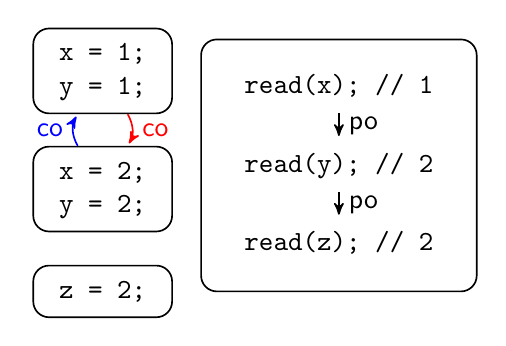
\begin{tikzpicture}[->,>=stealth',shorten >=1pt,auto,node distance=3cm,
     semithick, transform shape]
    \node[draw, rounded corners=2mm] (t1) at (0, .2) {\begin{tabular}{l} \texttt{x = 1;} \\ \texttt{y = 1;} \end{tabular}};
    \node[draw, rounded corners=2mm] (t2) at (0, -1.3) {\begin{tabular}{l} \texttt{x = 2;} \\ \texttt{y = 2;} \end{tabular}};
    \node[draw, rounded corners=2mm] (t3) at (0, -2.6) {\begin{tabular}{l} \texttt{z = 2;} \end{tabular}};
    \node[draw, rounded corners=2mm, minimum width=3.5cm, minimum height=3.2cm] (t4) at (3, -1) {};
    \node (t4_1) at (3, .0) {\begin{tabular}{l} \texttt{read(x); // 1} \end{tabular}};
    \node (t4_2) at (3, -1) {\begin{tabular}{l} \texttt{read(y); // 2} \end{tabular}};
    \node (t4_3) at (3, -2) {\begin{tabular}{l} \texttt{read(z); // 2} \end{tabular}};
    \path (t4_1) edge node {$\po$} (t4_2);
    \path (t1) edge[red, bend left] node {$\co$} (t2);
    \path (t4_2) edge node {$\po$} (t4_3);
    \path (t2) edge[blue, bend left] node {$\co$} (t1);
   \end{tikzpicture}  
  }
  \caption{Violation of \textsc{Read Atomic}}
  \label{ra_algo_counter_example:1}
 \end{subfigure}
  \hspace{.05cm}
 \begin{subfigure}{.29\textwidth}
  \resizebox{\textwidth}{!}{
   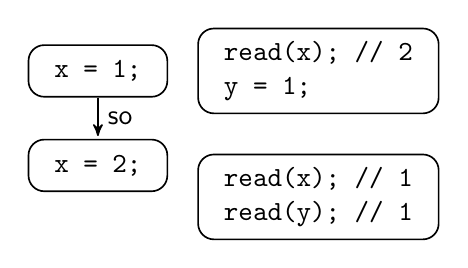
\begin{tikzpicture}[->,>=stealth',shorten >=1pt,auto,node distance=3cm,
     semithick, transform shape]
    \node[draw, rounded corners=2mm] (s11) at (0, 0) {\begin{tabular}{l} \texttt{x = 1;} \end{tabular}};
    \node[draw, rounded corners=2mm] (s12) at (0, -1.2) {\begin{tabular}{l} \texttt{x = 2;} \end{tabular}};
    \node[draw, rounded corners=2mm] (t1) at (2.8, 0) {\begin{tabular}{l} \texttt{read(x); // 2} \\ \texttt{y = 1;} \end{tabular}};
    \node[draw, rounded corners=2mm] (t2) at (2.8, -1.6) {\begin{tabular}{l} \texttt{read(x); // 1} \\ \texttt{read(y); // 1} \end{tabular}};
    \path (s11) edge node {$\so$} (s12);
    % \path (s11) edge[red, below] node {$\wro[\xvar]$} (t2);
    % \path (s12) edge[dashed, red, bend left] node {$\co$} (s11);
    % \path (s12) edge[red, bend right, left] node {$\wro^+$} (t2);
   \end{tikzpicture}  
  }
  \caption{Valid w.r.t. \textsc{Read Atomic}}
  \label{ra_algo_example:1}
 \end{subfigure}
 \hspace{.05cm}
 \begin{subfigure}{.36\textwidth}
  \resizebox{.93\textwidth}{!}{
   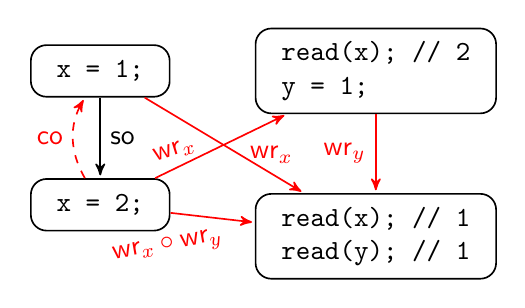
\begin{tikzpicture}[->,>=stealth',shorten >=1pt,auto,node distance=4cm,
     semithick, transform shape]
    \node[draw, rounded corners=2mm] (s11) at (0, 0) {\begin{tabular}{l} \texttt{x = 1;} \end{tabular}};
    \node[draw, rounded corners=2mm] (s12) at (0, -1.7) {\begin{tabular}{l} \texttt{x = 2;} \end{tabular}};
    \node[draw, rounded corners=2mm] (t1) at (3.5, 0) {\begin{tabular}{l} \texttt{read(x); // 2} \\ \texttt{y = 1;} \end{tabular}};
    \node[draw, rounded corners=2mm] (t2) at (3.5, -2.1) {\begin{tabular}{l} \texttt{read(x); // 1} \\ \texttt{read(y); // 1} \end{tabular}};
    \path (s11) edge node {$\so$} (s12);
    \path (s11) edge[red, right] node[pos=0.6] {$\wro[\xvar]$} (t2);
    \path (s12) edge[dashed, red, bend left] node {$\co$} (s11);
    \path (s12) edge[red, left,rotate=10] node[pos=.7,yshift=-6] {$\wro[\xvar] \circ \wro[\yvar]$} (t2);
    \path (s12) edge[red, left,rotate=17] node[pos=0.4,yshift=4] {$\wro[\xvar]$} (t1);
    \path (t1) edge[red, left] node {$\wro[\yvar]$} (t2);
   \end{tikzpicture}  
  }
  \caption{Violation of \textsc{Causal Consistency}}
  \label{cc_algo_counter_example:1}
 \end{subfigure}
 \caption{Applying the RA and CC checking algorithms.}
 \vspace{-3mm}
 \label{ptime_algo_examples}
\end{figure}


Intuitively, the polynomial time results are based on the fact that the axioms defining those consistency criteria do not contain the commit order ($\co$) on the left-hand side of the entailment. Therefore, proving the existence of a commit order satisfying those axioms can be done using a saturation procedure that builds a ``partial'' commit order based on instantiating the axioms on the write-read relation and the session order in the given history. Since the commit order must be an extension of the write-read relation and the session order, it contains those two relations from the beginning. 
This saturation procedure stops when the order constraints derived this way become cyclic. For instance, let us consider applying such a procedure corresponding to RA on the histories in Figure~\ref{ra_algo_counter_example:1} and Figure~\ref{ra_algo_example:1}. Applying the axiom in Figure~\ref{ra_def} on the first history, since the transaction on the right reads 2 from $\yvar$, we get that its $\wro[\xvar]$ predecessor (i.e., the first transaction on the left) must precede the transaction writing 2 to $\yvar$ in commit order (the red edge). This holds because the $\wro[\xvar]$ predecessor writes on $\yvar$. Similarly, since the same transaction reads 1 from $\xvar$, we get that its $\wro[\yvar]$ predecessor must precede the transaction writing 1 to $\xvar$ in commit order (the blue edge). This already implies a cyclic commit order, and therefore, this history does not satisfy RA. On the other hand, for the history in Figure~\ref{ra_algo_example:1}, all the axiom instantiations are vacuous, i.e., the left part of the entailment is false, and therefore, it satisfies RA. Checking CC on the history in Figure~\ref{cc_algo_counter_example:1} requires a single saturation step: since the transaction on the bottom right reads 1 from $\xvar$, its $\wro[\xvar]\circ\wro[\yvar]$ predecessor that writes on $\xvar$ (the transaction on the bottom left) must precede in commit order the transaction writing 1 to $\xvar$. Since this is already inconsistent with the session order, we get that this history violates CC.

\begin{algorithm}[t]
{\footnotesize
 \SetKwInOut{KwInput}{Input}
 \SetKwInOut{KwOutput}{Output}
 \KwIn{A history $\hist = \tup{T, \so, \wro}$}
 \KwOut{$\mathit{true}$ iff $\hist$ satisfies \textsc{Causal consistency}}
 \BlankLine
 \If{$\so\cup\wro$ is cyclic} {
  \Return{false}\;
 }
 $\co \leftarrow \so\cup\wro$\;
 \ForEach{$\xvar \in \vars{\hist}$}{
  \ForEach{$\tr_1 \neq \tr_2 \in T$ s.t. $\tr_1$ and $\tr_2$ write $\xvar$}{
   \If{$\exists \tr_3.\ \tup{\tr_1,\tr_3}\in \wro[\xvar]\land \tup{\tr_2,\tr_3}\in (\so\cup\wro)^+$} { %\Path{\tr_2}{E_1^+}{\tr_3}, \Path{\tr_1}{\wro[\xvar]}{\tr_3}
    $\co \leftarrow \co \cup \{\tup{\tr_2, \tr_1}\}$\;
   }
  }
 }
 \eIf{$\co$ is cyclic}{
  \Return{false}\;
 }{
  \Return{true}\;
 }}
 \caption{Checking \textsc{Causal consistency}.}
 \label{ccalgo:1}
\end{algorithm}

Algorithm~\ref{ccalgo:1} lists our procedure for checking CC. As explained above, $\CO$ is initially set to $\so\cup \wro$, and then, it is saturated with other ordering constraints implied by non-vacuous instantiations of the axiom $\mathsf{Causal}$ (where the left-hand side of the implication evaluates to true). The algorithms concerning RC and RA are defined in a similar way by essentially changing the test at line 6 so that it corresponds to the left-hand side of the implication in the corresponding axiom. Algorithm~\ref{ccalgo:1} can be rewritten as a Datalog program containing straightforward Datalog rules for computing transitive closures and relation composition, and a rule of the form\footnote{We write Datalog rules using a standard notation $\mathit{head}\text{ :- }\mathit{body}$ where $\mathit{head}$ is a relational atom (written as $\tup{a,b}\in R$ where $a$, $b$ are elements and $R$ a binary relation) and $\mathit{body}$ is a list of relational atoms.}
\begin{align*}
\tup{\tr_2, \tr_1} \in \CO \text{ :- } \tr_1\neq\tr_2, \tup{\tr_1,\tr_3}\in \wro[\xvar], \tup{\tr_2,\tr_3}\in (\so\cup\wro)^+
\end{align*}
to represent the $\mathsf{Causal}$ axiom.
%specification using the predicate from line 6-7; $\forall \tr_1, \tr_2, \tr_3.~uniq(\tr_1, \tr_2, \tr_3)$\footnote{$uniq(\tr_1, \tr_2, \tr_3) = \tr_1 \neq \tr_2 \land \tr_2 \neq \tr_3 \land \tr_3 \neq \tr_1$}~$\land \tup{\tr_1,\tr_3}\in \wro[\xvar]\land \tup{\tr_2,\tr_3}\in (\so\cup\wro)^+ \implies \tup{\tr_2, \tr_1} \in \CO$. 
The following is a consequence of the fact that these algorithms run in polynomial time (or equivalently, the corresponding Datalog programs can be evaluated in polynomial time over a database that contains the $\wro$ and $\so$ relations in a given history).%(see Appendix~\ref{app:sec:general}).
%The algorithms for checking \textsc{Read Committed}, \textsc{Read Atomic}, and \textsc{Causal Consistency} are given in Algorithm~\ref{} (TODO). 

\begin{theorem}
For any criterion $C \in \{\emph{\textsc{Read Committed}}, \emph{\textsc{Read Atomic}}, \emph{\textsc{Causal consistency}} \}$, 
the problem of checking whether a given history satisfies $C$ % \emph{\textsc{Read Committed}}, \emph{\textsc{Read Atomic}}, or \emph{\textsc{Causal consistency}} 
is polynomial time.
\end{theorem}

On the other hand, checking PC, SI, and SER is NP-complete in general. We show this using a reduction from boolean satisfiability (SAT) that covers uniformly all the three cases. In the case of SER, it provides a new proof of the NP-completeness result by \cite{DBLP:journals/jacm/Papadimitriou79b}, which uses a reduction from the so-called \emph{non-circular} SAT and which cannot be extended to PC and SI.

\begin{theorem}
 \label{npcproof:0}
\hspace{-2mm}
For any criterion $C \hspace{-.7mm}\in\hspace{-.7mm} \{\emph{\textsc{Prefix Consistency}},\hspace{-.5mm}\emph{\textsc{Snapshot Isolation}},\hspace{-.5mm}\emph{\textsc{Serializability}} \}$
the problem of checking whether a given history satisfies $C$ 
is NP-complete.
%The problem of checking whether a history satisfies any criteria between \emph{\textsc{Prefix Consistency}} and \emph{\textsc{Serializability}}, is NP-complete.
\end{theorem}
%!TEX root = Thesis.tex

\tikzset{transaction state /.style={draw=black!0}}
\begin{proof}
 Given a history, any of these three criteria %between \textsf{Prefix Consistency} and \textsf{Serializability} 
 can be checked by guessing a total commit order on its transactions and verifying whether it satisfies the corresponding axioms. This shows that the problem is in NP.
 
 To show NP-hardness, we define a reduction from boolean satisfiability. Therefore, let $\varphi=D_1\land\ldots\land D_m$ be a \textsf{CNF} formula over the boolean variables $x_1, \ldots, x_n$ where each $D_i$ is a disjunctive clause with $m_i$ literals.  %we reduce it to a history in polynominal time.
 Let $\lambda_{ij}$ denote the $j$-th literal of $D_i$. 
 
We construct a history $h_\varphi$ such that $\varphi$ is satisfiable if and only if $h_\varphi$ satisfies PC, SI, or SER. Since SER $\implies$ SI $\implies$ PC, we show that (1) if $h_\varphi$ satisfies PC, then $\varphi$ is satisfiable, and (2) if $\varphi$ is satisfiable, then $h_\varphi$ satisfies SER.

\paragraph{Construction of $h_\varphi$}
The main idea of the construction is to represent truth values of each of the variables and literals in $\varphi$ with the polarity of the commit order between corresponding transaction pairs.
For each variable $x_k$, $h_\varphi$ contains a pair of transactions $a_k$ and $b_k$, and for each literal $\lambda_{ij}$, $h_\varphi$ contains a set of transactions $w_{ij}$, $y_{ij}$ and $z_{ij}$\footnote{We assume that the transactions $a_k$ and $b_k$ associated to a variable $x_k$ are distinct and different from the transactions associated to another variable $x_{k'}\neq x_k$ or to a literal $\lambda_{ij}$. Similarly, for the transactions $w_{ij}$, $y_{ij}$ and $z_{ij}$ associated to a literal $\lambda_{ij}$.}. We want to have that $x_k$ is false if and only if $\tup{a_k, b_k} \in \CO$, and $\lambda_{ij}$ is false if and only if $\tup{y_{ij}, z_{ij}} \in \CO$ (the transaction $w_{ij}$ is used to "synchronize" the truth value of the literals with that of the variables, which is explained later).

The history $h_\varphi$ should ensure that the $\co$ ordering constraints corresponding to an assignment that falsifies the formula (\ie one of its clauses) form a cycle. 
%If for an assignment does not satisfy a clause, we want the corresponding relations to create a cycle in $\CO$. 
To achieve that, we add all pairs $\tup{z_{ij}, y_{i,(j+1)\% m_i}}$ in the session order $\so$. An unsatisfied clause $D_i$, \ie every $\lambda_{ij}$ is false, leads to a cycle of the form $y_{i1} \xrightarrow{\CO} z_{i1} \xrightarrow{\so} y_{i2} \xrightarrow{\co} z_{i2} \cdots z_{i m_i} \xrightarrow{\so} y_{i1}$.

\begin{figure}[t]
 \resizebox{\textwidth}{!}{
  \begin{subfigure}{.55\textwidth}
   \centering
   \begin{tikzpicture}[->,>=stealth',shorten >=1pt,auto,node distance=4cm,
     semithick, transform shape]
     % \node[transaction state,label={$\writeVar{}{v_j}$}] at (5, 2) (a_j)                                    {$a_j$};
    \node[transaction state] at (5, 2) (a_j)                                    {$a_k$};
    % \node[transaction state,label=below:{$\writeVar{}{v_j}$}] at (5,0)       (b_j)           {$b_j$};
    \node[transaction state] at (5,0)       (b_j)           {$b_k$};
    % \node[transaction state] at (-3,3)        (c_j)                     {$c_j$};
    \node[transaction state] at (4,0)        (w_ik)                     {$w_{ij}$};
    \node[transaction state,label={$\writeVar{}{v_{ij}}$}] at (2,2) (y_ik) {$y_{ij}$};
    \node[transaction state] at (2,0) (z_ik) {$z_{ij}$};
    \node[transaction state] at (.5,2.5) (z_ik1) {$z_{i,j-1}$};
    \node[transaction state] at (.5, -.5) (y_ik1) {$y_{i,j+1}$};
    
    \path (a_j) edge[dotted, red, bend left=25] node {\CO} (b_j)
    (b_j) edge[dashed, red, bend left=25] node {\CO} (a_j);
    % (b_j) edge[bend left] node {\WR} (c_j)
    % (c_j) edge[dashed, red, bend left] node {\RW} (a_j);
    
    \path (y_ik) edge[dotted, blue, bend left=25] node {\CO} (z_ik)
    (z_ik) edge[dashed, blue, bend left=25] node {\CO} (y_ik)
    (z_ik) edge node {$\wro[v_{ij}]$} (w_ik);
    % (w_ik) edge[dashed, blue, bend left] node {\RW} (y_ik);
    
    \path (y_ik) edge node {$\so$} (a_j)
    (b_j) edge node[above] {$\so$} (w_ik)
    (z_ik1) edge node[below] {$\so$} (y_ik)
    (z_ik) edge node {$\so$} (y_ik1);
   \end{tikzpicture}
   \caption{$\lambda_{ij} = x_k$}
   \label{fig:lambda_i_k_x_j_}
  \end{subfigure}
  \begin{subfigure}{.55\textwidth}
   \centering
   \begin{tikzpicture}[->,>=stealth',shorten >=1pt,auto,node distance=4cm,
     semithick, transform shape]
     % \node[transaction state,label={$\writeVar{}{v_j}$}] at (5, 2) (b_j)                                    {$b_j$};
    \node[transaction state] at (5, 2) (b_j)                                    {$b_k$};
    % \node[transaction state,label=below:{$\writeVar{}{v_j}$}] at (5,0)       (a_j)           {$a_j$};
    \node[transaction state] at (5,0)       (a_j)           {$a_k$};
    % \node[transaction state] at (-3,3)        (c_j)                     {$c_j$};
    \node[transaction state] at (4,0)        (w_ik)                     {$w_{ij}$};
    \node[transaction state,label={$\writeVar{}{v_{ij}}$}] at (2,2) (y_ik) {$y_{ij}$};
    \node[transaction state] at (2,0) (z_ik) {$z_{ij}$};
    \node[transaction state] at (.5,2.5) (z_ik1) {$z_{i,j-1}$};
    \node[transaction state] at (.5, -.5) (y_ik1) {$y_{i,j+1}$};
    
    \path (a_j) edge[dashed, red, bend left=25] node {\CO} (b_j)
    (b_j) edge[dotted, red, bend left=25] node {\CO} (a_j);
    % (b_j) edge[bend right] node {\WR} (c_j)
    % (c_j) edge[dashed, red, bend right] node {\RW} (a_j);
    
    \path (y_ik) edge[dotted, blue, bend left=25] node {\CO} (z_ik)
    (z_ik) edge[dashed, blue, bend left=25] node {\CO} (y_ik)
    (z_ik) edge node {$\wro[v_{ij}]$} (w_ik);
    % (w_ik) edge[dashed, blue, bend left] node {\RW} (y_ik);
    
    \path (y_ik) edge node {$\so$} (b_j)
    (a_j) edge node[above] {$\so$} (w_ik)
    (z_ik1) edge node[below] {$\so$} (y_ik)
    (z_ik) edge node {$\so$} (y_ik1);
   \end{tikzpicture}
   \caption{$\lambda_{ij} = \neg x_k$}
   \label{fig:lambda_i_k_n_x_j_}
  \end{subfigure}
 }
  \vspace{-2mm}
 \caption{Sub-histories included in $h_\varphi$ for each literal $\lambda_{ij}$ and variable $x_k$.}
 \vspace{-3mm}
\end{figure}

The most complicated part of the construction is to ensure some consistency between the truth value of the literals and the truth value of the variables, e.g., $\lambda_{ij} = x_k$ is true iff $x_k$ is true, for at least one literal $\lambda_{ij}$ interpreted as true in every clause $D_i$ (if such a literal exists).
Figure~\ref{fig:lambda_i_k_x_j_} shows the sub-history associated to a positive literal $\lambda_{ij} = x_k$ while Figure~\ref{fig:lambda_i_k_n_x_j_} shows the case of a negative literal $\lambda_{ij} = \neg x_k$.
For a positive literal $\lambda_{ij} = x_k$ (Figure~\ref{fig:lambda_i_k_x_j_}), (1) we enrich session order with the pairs $\tup{y_{ij}, a_k}$ and $\tup{b_k, w_{ij}}$, (2) we include writes to a variable $v_{ij}$ in the transactions $y_{ij}$ and $z_{ij}$, and (3) we make $w_{ij}$ read from $z_{ij}$, $\ie$ $\tup{z_{ij}, w_{ij}}\in \wro_{v_{ij}}$. The case of a negative literal is similar, switching the roles of $a_k$ and $b_k$.

\paragraph{PC for $h_\varphi$ implies satisfiability of $\varphi$}
If $h_\varphi$ satisfies PC, then there exists a total commit order $\co$ between the transactions described above, which together with $h_\varphi$ satisfies $\mathsf{Prefix}$. We show that the assignment of the variables $x_k$ explained above (defined by the $\co$ order between $a_k$ and $b_k$, for each $k$) satisfies the formula $\varphi$. For each clause $D_i$, the $\so$ constraints between the transactions $y_{ij}$, $z_{ij}$ with $1\leq j\leq m_i$ imply that there exist some $z_{ij}$ that is committed before its corresponding $y_{ij}$. These two transactions are included in the sub-history corresponding to the literal $\lambda_{ij}$ (Figure~\ref{fig:lambda_i_k_x_j_} or Figure~\ref{fig:lambda_i_k_n_x_j_} depending on the polarity of the literal).
% and their order in $\co$ implies t

The definition of this sub-history ensures that the interpretation to true of the literal $\lambda_{ij}$ (given by the order in $\co$ between $z_{ij}$ and $y_{ij}$) is consistent with the assignment of the variable it contains (defined by the $\co$ order between $a_k$, $b_k$). More precisely, it ensures that if the $\co$ goes upwards on the left-hand side ($\tup{z_{ij}, y_{ij}} \in \co$) like in this case, then it must also go upwards on the right-hand side ($\tup{b_k, a_k} \in \co$ in the case of a positive literal, and $\tup{a_k, b_k} \in \co$ in the case of a negative literal) to satisfy $\mathsf{Prefix}$. For instance, if $\lambda_{ij}=x_k$ is a positive literal and we assume by contradiction that $\tup{a_k, b_k} \in \co$, then $\tup{y_{ij}, w_{ij}} \in \so \circ \co \circ \so$. Therefore, for every commit order $\CO$ such that $\tup{h_\varphi,\co}$ satisfies $\mathsf{Prefix}$, $\tup{a_k, b_k} \in \CO$ implies $\tup{y_{ij}, z_{ij}} \in \co$, which contradicts the hypothesis. Indeed, if $\tup{a_k, b_k} \in \CO$, instantiating the $\mathsf{Prefix}$ axiom  where $y_{ij}$ plays the role of $t_2$, $z_{ij}$ plays the role of $t_1$, and $w_{ij}$ plays the role of $t_3$, we obtain that $\tup{y_{ij}, z_{ij}} \in \co$. 

Therefore, the assignment of the variables $x_k$ leads to at least one literal interpreted to true in each clause $D_i$, and the formula $\varphi$ is satisfiable.

%right-hand side ($\tup{a_k, b_k} \in \co$ in the case of a positive literal, and $\tup{b_k, a_k} \in \co$ in the case of a negative literal), then it must also go downwards on the left-hand side ($\tup{y_{ij}, z_{ij}} \in \co$) to satisfy $\mathsf{Prefix}$.
%
%
%By the design of the sub-history corresponding to $\lambda_{ij}$
%
% since there exists no cycle between the transactions $y_{ij}$ and $z_{ij}$, which implies that for each clause $D_i$, there exists a $j$ such that $\tup{y_{ij}, z_{ij}} \not \in \CO$ which means that $\lambda_{ij}$ is satisfied.
%
%
%We use special sub-histories to enforce that if history $h_\varphi$ satisfies PC (i.e., the axiom $\mathsf{Prefix}$), 
%%any criteria between \textsf{Prefix Consistency} and \textsf{Serializability}, 
%then there exists a commit order $\CO$ such that $\tup{h_\varphi,\co}$ satisfies $\mathsf{Prefix}$ (Figure~\ref{pre_def}) and:
%\begin{align}
%\mbox{$\tup{a_k, b_k} \in \CO$ iff $\tup{y_{ij}, z_{ij}} \in \CO$ when $\lambda_{ij} = x_k$, and }\label{eq:iffs}\\
%\mbox{$\tup{a_k, b_k} \in \CO$ iff $\tup{z_{ij}, y_{ij}} \in \CO$ when $\lambda_{ij} = \neg x_k$}.\nonumber
%\end{align}
%%provided that the history $h_\varphi$ satisfies any criteria between \textsf{Prefix Consistency} and \textsf{Serializability}.
%%
%%We will particularly show if $\varphi_\hist$ satisfies \textsf{Prefix Consistency}(weakest criteria), then the $\varphi$ is satisfiable and if $\varphi$ is satisfiable, then $\varphi_\hist$ satisfies \textsf{Serializability}(strongest criteria).
%%
%%Now the truth value of each $\lambda_{ik} = x_j$ or $\neg x_j$ has a consistent truth value according to the truth value of $x_j$. We use special subhistories to enforce the equivalent consistency between $\tup{y_{ik}, z_{ik}}$ and $\tup{a_j, b_j}$.
%%
%%These sub-histories are shown in Figure~\ref{fig:lambda_i_k_x_j_} and Figure~\ref{fig:lambda_i_k_n_x_j_}. 
%%show the special subhistories for each $\lambda_{ik} = x_j$ and $\lambda_{ik} = \neg x_j$ respectively. 
%%
%
%
%This construction ensures that if the $\co$ goes downwards on the right-hand side ($\tup{a_k, b_k} \in \co$ in the case of a positive literal, and $\tup{b_k, a_k} \in \co$ in the case of a negative literal), then it must also go downwards on the left-hand side ($\tup{y_{ij}, z_{ij}} \in \co$) to satisfy $\mathsf{Prefix}$. For instance, in the case of a positive literal, note that if $\tup{a_k, b_k} \in \co$, then $\tup{y_{ij}, w_{ij}} \in \so \circ \co \circ \so$. Therefore, for every commit order $\CO$ such that $\tup{h_\varphi,\co}$ satisfies $\mathsf{Prefix}$, $\tup{a_k, b_k} \in \CO$ implies $\tup{y_{ij}, z_{ij}} \in \co$. Indeed, if $\tup{a_k, b_k} \in \CO$, instantiating the $\mathsf{Prefix}$ axiom  where $y_{ij}$ plays the role of $t_2$, $z_{ij}$ plays the role of $t_1$, and $w_{ij}$ plays the role of $t_3$, we obtain that $\tup{y_{ij}, z_{ij}} \in \co$. 
%
%In contrast, when the $\co$ goes upwards on the right-hand side ($\tup{b_k, a_k} \in \co$ in the case of a positive literal, and $\tup{a_k, b_k} \in \co$ in the case of a negative literal) then it imposes no constraint on the direction of $\co$ on the left-hand side. Therefore, any commit order $\co$ satisfying $\mathsf{Prefix}$ that goes upwards on the right-hand side (e.g., $\tup{b_k, a_k} \in \co$ in the case of a positive literal) and downwards on the left-hand side ($\tup{y_{ij}, z_{ij}} \in \co$) in some sub-history (associated to some literal), thereby contradicting Property (\ref{eq:iffs}), can be modified into another commit order satisfying $\mathsf{Prefix}$ that goes upwards on the left-hand side as well. Formally, let $\CO$ be a commit order such that $\tup{h_\varphi,\co}$ satisfies $\mathsf{Prefix}$ and 
%\begin{align*}
%\tup{b_k, a_k} \in \CO \land \tup{y_{ij}, z_{ij}} \in \CO
%\end{align*}
%for some literal $\lambda_{ij} = x_k$ (the case of negative literals can be handled in a similar manner). Let $\CO_1$ be the restriction of $\CO$ on the set of tuples 
%\begin{align*}
%\{\tup{a_{k'}, b_{k'}}, \tup{b_{k'}, a_{k'}} | 1\leq k'\leq n\} \cup \{\tup{y_{i'j'}, z_{i'j'}}, \tup{z_{i'j'}, y_{i'j'}} | \text{for each }i', j'\} \cup \so \cup \wro. 
%\end{align*}
%Since $\CO_1 \subseteq \CO$, we have that $\CO_1$ is acyclic. 
%%Let $\lambda_{ij} = x_k$ be a literal such that $\tup{y_{ij}, z_{ij}} \in \CO_1$ and $\tup{b_k, a_k} \in \CO_1$. 
%Let $\CO_2$ be a relation obtained from $\CO_1$ by flipping the order between $y_{ij}$ and $z_{ij}$ (\ie $\CO_2 = \CO_1 \setminus \{ \tup{y_{ij}, z_{ij}} \} \cup \{ \tup{z_{ij}, y_{ij}} \}$). This flipping does not introduce any cycle because $\CO_2$ contains no path ending in $z_{ij}$ (see Fig~\ref{fig:lambda_i_k_x_j_}). Also, $\CO_2$ still satisfies the $\mathsf{Prefix}$ axiom (since $\tup{b_k, a_k} \in \CO_2$ there is no path from $y_{ij}$ to $w_{ij}$ satisfying the constraints in the $\mathsf{Prefix}$ axiom). Since $\CO_2$ is acyclic, it can be extended to a total commit order $\CO_3$ that satisfies $\mathsf{Prefix}$. This is a consequence of the following lemma whose proof follows easily from definitions (the part of this lemma concerning $\mathsf{Serializability}$ will be used later).%Moreover, $\CO_3$ has strictly less literals $\lambda_{ij} = x_k$ satisfying $\tup{y_{ij}, z_{ij}} \in \CO \land \tup{b_k, a_k} \in \CO$ than $\CO$, which contradicts the hypothesis.
%
%\begin{lemma}\label{lem:extensions}
%Let $\co$ be an acyclic relation that includes $\so\cup\wro$, $\tup{a_{k}, b_{k}}$ or $\tup{b_{k}, a_{k}}$, for each $k$, and $\tup{y_{ij},z_{ij}}$ or $\tup{z_{ij},y_{ij}}$, for each $i$, $j$. For each axiom $A\in \{\mathsf{Prefix}, \mathsf{Serializability}\}$, if $\tup{h_\varphi,\co}$ satisfies $A$, then there exists a total commit order $\co'$ such that $\co\subseteq \co'$ and $\tup{h_\varphi,\co'}$ satisfies $A$.
%\end{lemma}
%
%Therefore, $\tup{h_\varphi,\co_3}$ satisfies $\mathsf{Prefix}$, and $\tup{b_k, a_k} \in \CO_3 \land \tup{z_{ij}, y_{ij}} \in \CO_3$ ($\co_3$ goes upwards on both sides of a sub-history like in Figure~\ref{fig:lambda_i_k_x_j_}). This transformation can be applied iteratively until obtaining a commit order that satisfies both $\mathsf{Prefix}$ and Property (\ref{eq:iffs}).
%
%%Furthermore, if $h_\varphi$ satisfies PC, then it satisfies $\mathsf{Prefix}$. The axiom imply that $\tup{y_{ij}, z_{ij}} \in \co$ ($y_{ij}$ plays the role of $t_2$, $z_{ij}$ plays the role of $t_1$, and $w_{ij}$ plays the role of $t_3$ in Figure~\ref{pre_def} and Figure~\ref{ser_def}, respectively). This is proved for all witnessing commit orders $\CO$.
%
%%Now to prove that there exists a commit order $\CO$ such that $\tup{y_{ij}, z_{ij}} \in \CO$ implies $\tup{a_k, b_k} \in \CO$ if $\lambda_{ij} = x_k$. Assume by contradiction that there exists no such commit order. Let $\CO$ be a commit order satisfying the PC axioms in which the number of literals $\lambda_{ij} = x_k$ satisfying $\tup{y_{ij}, z_{ij}} \in \CO \land \tup{b_k, a_k} \in \CO$ (ie. the violation of $\tup{y_{ij}, z_{ij}} \in \CO$ implies $\tup{a_k, b_k} \in \CO$) is minimal. Let $\CO_1$ be the restriction of $\CO$ on the set of tuples $\{\tup{a_k, b_k}, \tup{b_k, a_k} | \text{for each }k\} \cup \{\tup{y_{ij}, z_{ij}}, \tup{z_{ij}, y_{ij}} | \text{for each }i, j\} \cup \so \cup \wro$. Since $\CO_1 \subseteq \CO$, we have that $\CO_1$ is acyclic. Let $\lambda_{ij} = x_k$ be a literal such that $\tup{y_{ij}, z_{ij}} \in \CO_1$ and $\tup{b_k, a_k} \in \CO_1$. Let $\CO_2$ be a relation obtained from $\CO_1$ by flipping the order between $y_{ij}$ and $z_{ij}$ (\ie $\CO_2 = \CO_1 \setminus \{ \tup{y_{ij}, z_{ij}} \} \cup \{ \tup{z_{ij}, y_{ij}} \}$). This flipping does not introduce any cycle because $\CO_2$ contains no path ending in $z_{ij}$ (see Fig~\ref{fig:lambda_i_k_x_j_}). Also, $\CO_2$ still satisfies the PC axiom (since $\tup{b_k, a_k} \in \CO$ there is no path from $y_{ij}$ to $w_{ij}$ satisfying the constraints in the PC axiom). Since $\CO_2$ is acyclic, it can be extended to a total commit order $\CO_3$ that satisfies the PC axiom. Moreover, $\CO_3$ has strictly less literals $\lambda_{ij} = x_k$ satisfying $\tup{y_{ij}, z_{ij}} \in \CO \land \tup{b_k, a_k} \in \CO$ than $\CO$, which contradicts the hypothesis.
%%
%%For the case of $\lambda_{ij} = \neg x_k$ in figure~\ref{fig:lambda_i_k_n_x_j_}, $\tup{b_k, a_k} \in \CO$ implies $\tup{y_{ij}, z_{ij}} \in \CO$ for any witnessing $\CO$. This direction can be proved similarly as the case of $\lambda_{ij} = x_k$ switching the roles of $a_k$ and $b_k$.
%%
%%Also, to prove that there exists a commit order $\CO$ such that $\tup{y_{ij}, z_{ij}} \in \CO$ implies $\tup{b_k, a_k} \in \CO$ if $\lambda_{ij} = \neg x_k$, we use the similar argument as $\lambda_{ij} = x_k$ switching the roles of $a_k$ and $b_k$. Only we start with a $\CO$ which does not include any violation of $\tup{y_{ij}, z_{ij}} \in \CO$ implies $\tup{a_k, b_k} \in \CO$ (we proved such $\CO$ exists) and prove existence of a $\CO'$ which does not contain any violation of $\tup{y_{ij}, z_{ij}} \in \CO$ implies $\tup{b_k, a_k} \in \CO$ if $\lambda_{ij} = \neg x_k$. While constructing the cases of $\lambda_{ij} = x_k$ remain same as $\CO$. So $\CO'$ also does not contain any violation of $\tup{y_{ij}, z_{ij}} \in \CO$ implies $\tup{a_k, b_k} \in \CO$ if $\lambda_{ij} = x_k$.
%
%%We can do a similar construction in figure \ref{fig:lambda_i_k_n_x_j_}, but we reverse the role of $a_j$ and $b_j$.
%
%%In figure \ref{fig:lambda_i_k_x_j_}, if $\tup{a_j, b_j} \in \co$, then $\tup{y_{ik}, w_{ik}} \in \so \circ \co \circ \so$. So by the axioms of SER, SI and PC in table \ref{consistency_defs}, $\tup{y_{ik}, z_{ik}} \in \co$. Similarly we can argue about the case of $\lambda_{ik} = \neg x_j$ in figure \ref{fig:lambda_i_k_n_x_j_} by reversing the role of $a_j$ and $b_j$.
%%
%%If $h_\varphi$ is SER, SI or PC, these subhistoies will enforce,
%%
%%\begin{itemize}
%% \item If $\lambda_{ik} = x_j$, $\tup{a_j, b_j} \in \CO$ would imply $\tup{y_{ik}, z_{ik}} \in CO$ in $h_\varphi$.
%% \item If $\lambda_{ik} = \neg x_j$, $\tup{a_j, b_j} \not\in \CO$ $\ie$ $\tup{b_j, a_j} \in \CO$ would imply $\tup{y_{ik}, z_{ik}} \in CO$.
%%\end{itemize}
%
%Next, we complete the correctness proof of this reduction. % \ie $\varphi$ is satisfiable if and only if $h_\varphi$ satisfies any criteria between PC and SER. 
%For the ``if'' direction, if $h_\varphi$ satisfies PC, then there exists a total commit order $\co$ between the transactions described above, which together with $h_\varphi$ satisfies $\mathsf{Prefix}$. The assignment of the variables $x_k$ explained above (defined by the $\co$ order between $a_k$ and $b_k$, for each $k$) satisfies the formula $\varphi$ since there exists no cycle between the transactions $y_{ij}$ and $z_{ij}$, which implies that for each clause $D_i$, there exists a $j$ such that $\tup{y_{ij}, z_{ij}} \not \in \CO$ which means that $\lambda_{ij}$ is satisfied.

\paragraph{Satisfiability of $\varphi$ implies SER for $\hist_\varphi$}
Let $\gamma$ be a satisfying assignment for $\varphi$. Also, let $\CO'$ be a binary relation that includes $\so$ and $\wro$ such that if $\gamma(x_k)=\mathit{false}$, then $\tup{a_k, b_k} \in \CO'$, $\tup{y_{ij}, z_{ij}} \in \CO'$ for each $\lambda_{ij} = x_k$, and $\tup{z_{ij}, y_{ij}} \in \CO'$ for each $\lambda_{ij} = \neg x_k$, and if $\gamma(x_k)=\mathit{true}$, then $\tup{b_k, a_k} \in \CO'$, $\tup{z_{ij}, y_{ij}} \in \CO'$ for each $\lambda_{ij} = x_k$, and $\tup{y_{ij}, z_{ij}} \in \CO'$ for each $\lambda_{ij} = \neg x_k$. Looking at the sub-histories corresponding to literals $\lambda_{ij}$ (Figure~\ref{fig:lambda_i_k_x_j_} or Figure~\ref{fig:lambda_i_k_n_x_j_}), $\co'$ goes in the same direction (upwards or downwards) on both sides. 

Note that $\CO'$ is acyclic: no cycle can contain $w_{ij}$ because $w_{ij}$ has no ``outgoing'' dependency (\ie $\CO'$ contains no pair with $w_{ij}$ as a first component), there is no cycle including some pair of transactions $a_k$, $b_k$ and some pair $y_{ij}$, $z_{ij}$ because there is no way to reach $y_{ij}$ or $z_{ij}$ from $a_k$ or  $b_k$, there is no cycle including only transactions $a_k$ and $b_k$ because $a_{k_1}$ and $b_{k_1}$ are not related to $a_{k_2}$ and $b_{k_2}$, for $k_1\neq k_2$, there is no cycle including transactions $y_{i_1,j_1}$, $z_{i_1,j_1}$ and $y_{i_2,j_2}$, $z_{i_2,j_2}$ for $i_1\neq i_2$ since these are disconnected as well, and finally, there is no cycle including only transactions $y_{ij}$ and $z_{ij}$, for a fixed $i$, because $\varphi$ is satisfiable. It can be proved easily that the acyclic relation $\co'$ can be extended to a total commit order $\co$ which together with $h_\varphi$ satisfies the $\mathsf{Serializability}$ axiom. Therefore, $h_\varphi$ satisfies SER.
%
%TODO I STOPPED HERE
%
%Also, there is no cycle in $\co$. So there is no cycle of the form $y_{i1} \xrightarrow{\CO} z_{i1} \xrightarrow{\so} y_{i2} \cdots z_{ik} \xrightarrow{\so} y_{i1}$ for any $i$. So each clause $i$ has a $k$ such that $\tup{y_{ik}, z_{ik}} \not\in \co$ which implies there exists an assignment(given by $\tup{a_j, b_j}$) for which each clause is satisfied. Thus $\varphi$ is satisfiable.
%
%For the other direction, we show, there no other kind of cycle is possible in $h_\varphi$, when $\tup{y_{ik}, z_{ik}}$ and $\tup{a_j, b_j}$ pairs are fixed.
%\begin{itemize}
% \item First note, no cycle can contain $w_{ik}$ because it does not have any outgoing relation(TODO better word). 
% \item Also it is easy to see, there is no cycle involving both $a_j, b_j, y_{ik}, z_{ik}$ because there is no way to reach $y_{ik}, z_{ik}$ from any $a_j, b_j$. 
% \item $a_j, b_j$ can not have cycles because each of $a_{j1}, b_{j1}$ and $a_{j2}, b_{j2}$ are disconnected. 
% \item Each of $y_{i1k1}, z_{i1k1}$ and $y_{i2k2}, z_{i2k2}$ are also disconnected.
%\end{itemize}
%
%So only possible cycle is in $y_{ik}, z_{ik}$ for each clause $i$. But, given an satisfying assignment of $\phi$, we can set $\tup{a_j, b_j}$ and $\tup{y_{ik}, z_{ik}}$ accordingly. Since every clause $i$ is satisfied, there is at least one $\tup{y_{ik}, z_{ik}} \not\in \co$ \ie there is no cycle in $y_{ik}, z_{ik}$. Hence, we can extend that strict partial order to a total order $\CO$. Thus, $h_\varphi$ is PC, SI or SER.
\end{proof}

\section{Checking Consistency of Bounded-Width Histories}\label{sec:bounded_width}

% Given a history it takes polynomial time to check for \textsc{Int} and \textsf{Ext}. Transactions, in a read atomic consistent history, can be assumed to read and write each variable at max once - just take the first read and last write of each variable. So for the rest of the paper, we will assume this.

In this section, we show that checking prefix consistency, snapshot isolation, and serializability becomes polynomial time under the assumption that the \emph{width} of the given history, i.e., the maximum number of mutually-unordered transactions w.r.t. the session order, is bounded by a fixed constant. If we consider the standard case where the session order is a union of transaction sequences (modulo the fictitious transaction writing the initial values), i.e., a set of sessions, then the width of the history is the number of sessions. We start by presenting an algorithm for checking serializability that is polynomial time when the width is bounded by a fixed constant. In general, the asymptotic complexity of this algorithm is exponential in the width of the history, but this worst-case behavior is not exercised in practice as shown in Section~\ref{sec:exp}. Then, we prove that checking prefix consistency and snapshot isolation can be reduced in polynomial time to the problem of checking serializability. 

% \subsection{Serialization and Linearization}
\subsection{Checking Serializability}\label{ssec:ser_checking}

We present an algorithm for checking serializability of a given history which constructs a valid commit order (satisfying $\mathsf{Serialization}$), if any, by 
``linearizing'' transactions one by one in an order consistent with the session order. At any time, the set of already linearized transactions is uniquely determined by an antichain of the session order (i.e., a set of mutually-unordered transactions w.r.t. $\so$), and the next transaction to linearize is chosen among the immediate $\so$ successors of the transactions in this antichain. The crux of the algorithm is that the next transaction to linearize can be chosen such that it does not produce violations of $\mathsf{Serialization}$ in a way that  does not depend on the order between the already linearized transactions. Therefore, the algorithm can be seen as a search in the space of $\so$ antichains. If the width of the history is bounded (by a fixed constant), then the number of possible $\so$ antichains is polynomial in the size of the history, which implies that the search can be done in polynomial time.

\begin{figure}
  
  \begin{subfigure}{.4\textwidth}
  \resizebox{\textwidth}{!}{
  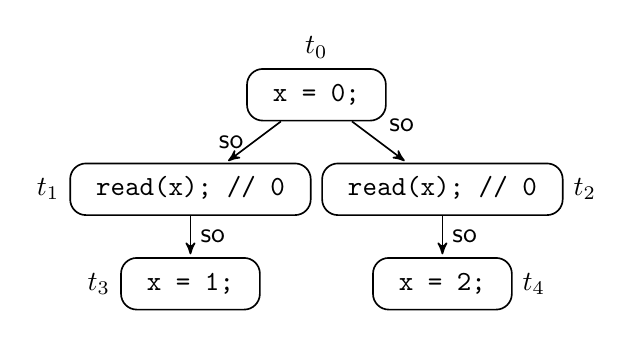
\begin{tikzpicture}[->,>=stealth',shorten >=1pt,auto,node distance=3cm,
   semithick, transform shape]
   \node[draw, rounded corners=2mm,label={$\tr_0$}] (t1) at (0, 1.2) {\begin{tabular}{l} \texttt{x = 0;} \end{tabular}};
   \node[draw, rounded corners=2mm,label=left:{$\tr_1$}] (t2r) at (-1.6, 0) {\begin{tabular}{l} \texttt{read(x); // 0} \end{tabular}};
   \node[draw, rounded corners=2mm,label=left:{$\tr_3$}] (t2w) at (-1.6, -1.2) {\begin{tabular}{l}  \texttt{x = 1;} \end{tabular}};
   \node[draw, rounded corners=2mm,label=right:{$\tr_2$}] (t3r) at (1.6, 0) {\begin{tabular}{l} \texttt{read(x); // 0} \end{tabular}};
   \node[draw, rounded corners=2mm,label=right:{$\tr_4$}] (t3w) at (1.6, -1.2) {\begin{tabular}{l} \texttt{x = 2;} \end{tabular}};
  \path (t2r) edge node {$\so$} (t2w);
  \path (t3r) edge node {$\so$} (t3w);
  \path (t1) edge node[left] {$\so$} (t2r);
  \path (t1) edge node {$\so$} (t3r);
  \end{tikzpicture}  
  }
   \caption{ }
   \label{ser_algo_example:1}
  \end{subfigure}
  \hspace{1cm}
   \begin{subfigure}{.19\textwidth}
    \resizebox{\textwidth}{!}{
     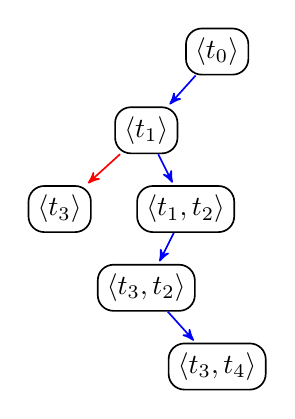
\begin{tikzpicture}[->,>=stealth',shorten >=1pt,auto,node distance=3cm,
       semithick, transform shape]
      \node[draw, rounded corners=2mm] (v00) at (0, 0) {$\left\langle \tr_0 \right\rangle$};
      \node[draw, rounded corners=2mm] (v10) at (-.9, -1) {$\left\langle \tr_1  \right\rangle$};
      \node[draw, rounded corners=2mm] (v20) at (-2, -2) {$\left\langle \tr_3 \right\rangle$};
      \node[draw, rounded corners=2mm] (v11) at (-.4, -2) {$\left\langle \tr_1, \tr_2  \right\rangle$};
      \node[draw, rounded corners=2mm] (v21) at (-.9, -3) {$\left\langle \tr_3, \tr_2  \right\rangle$};
      \node[draw, rounded corners=2mm] (v22) at (0, -4) {$\left\langle \tr_3, \tr_4  \right\rangle$};
      % \pic (v10) at (-3.5, -4)    {ser_history=v10};
      % \pic (v20) at (-7, -8)    {ser_history=v20};
      % \pic (v11) at (0, -8)    {ser_history=v11};
      % \pic (v21) at (-3.5, -12)    {ser_history=v21};
      % \pic (v22) at (0, -16)    {ser_history=v22};
      \path (v00) edge[blue] node {} (v10); 
      \path (v10) edge[red] node {} (v20); 
      \path (v10) edge[blue] node {} (v11); 
      \path (v11) edge[blue] node {} (v21); 
      \path (v21) edge[blue] node {} (v22);
      
      % \draw[-, blue, dashed] plot[smooth, tension=2] coordinates { (-1.5,1.5) (0, .5) (1.5, 1.5)};
      % \draw[-, blue, dashed] plot coordinates { (-1.2,1.7) (-1.2, .7) (1.2, .7) (1.2, 1.7)};
      % \draw[-, blue, dashed] plot coordinates { (-7,-2.3) (-7,-4.5) (-3.5,-4.5) (-3.5,-3.5) (-1.5,-3.5) (-1.5,-2.3) };
      % \draw[-, blue, dashed] plot coordinates { (-3.5,-6.3) (-3.5,-8.5) (3.4,-8.5) (3.4,-6.3) };
      % % \draw[-, blue, dashed] plot coordinates { (-10.5,-6.5) (-10.5,-10) (-7, -10) (-7, -7.5) (-3.6,-7.5) (-3.6,-6.5) };
      % \draw[-, blue, dashed] plot coordinates { (-10.5,-6.3) (-10.5,-8.5) };
      % \draw[-, red, dashed] plot coordinates { (-10.5,-8.5) (-10.5,-10) (-7,-10) (-7, -8.5) };
      % \draw[-, blue, dashed] plot coordinates { (-7, -8.5) (-7, -7.5) (-3.6,-7.5) (-3.6,-6.3) };
      % \draw[-, blue, dashed] plot coordinates { (-7,-10.3) (-7,-14) (-3.5, -14) (-3.5, -12.5) (-.1,-12.5) (-.1,-10.3) };
      % \draw[-, blue, dashed] plot coordinates { (-3.5,-14.3) (-3.5,-17.9) (3.4, -17.9) (3.4,-14.3) };
      % \draw[-, blue, dashed] plot coordinates { (-10.5,-6.5) (-10.5,-8.5) (-3.5,-8.5) (-3.5,-6.5) };
      
     \end{tikzpicture}  
    }
    \caption{ }
    \label{ser_algo_example:3}
   \end{subfigure}
   \vspace{-4mm}
  \caption{Applying the serializability checking algorithm \textsf{checkSER} (Algorithm~\ref{seralgo:2}) on the serializable history on the left. The right part pictures a search for valid extensions of serializable prefixes, represented by their boundaries. The red arrow means that the search is blocked (the prefix at the target is not a valid extension), while blue arrows mean that the search continues.}
  \label{ser_algo_example}
  \vspace{-4mm}
\end{figure}

A \emph{prefix} of a history $\hist = \tup{T, \so, \wro}$ is a set of transactions $T'\subseteq T$ such that all the $\so$ predecessors of transactions in $T'$ are also in $T'$, i.e., $\forall \tr\in T.\ \so^{-1}(\tr)\in T$. A prefix $T'$ is uniquely determined by the set of transactions in $T'$ that are maximal w.r.t. $\so$. This set of transactions forms an \emph{antichain} of $\so$, i.e., any two elements in this set are incomparable w.r.t. $\so$. Given an antichain $\{\tr_1,\ldots,\tr_n\}$ of $\so$, we say that $\{\tr_1,\ldots,\tr_n\}$ is the \emph{boundary} of the prefix $T'=\{t:\exists i.\ \tup{t,t_i}\in \so\lor t = t_i\}$. For instance, given the history in Figure~\ref{ser_algo_example:1}, the set of transactions $\{\tr_0,\tr_1,\tr_2\}$ is a prefix with boundary $\{\tr_1,\tr_2\}$ (the latter is an antichain of the session order).

%TODO SHOW THE ALGORITHM RUNNING ON A HISTORY: GIVE A SERIALIZABLE HISTORY, A GRAPH WHERE NODES ARE ANTICHAINS AND EDGES ARE "VALID EXTENSION" (WE SHOULD HAVE SOME PATH THAT BLOCKS, AN ANTICHAIN WHICH CANNOT BE EXTENDED). FOR HERE, CIRCLE A PREFIX ON THAT HISTORY AND REFER TO IT.

A prefix $T'$ of a history $\hist$ is called \emph{serializable} iff there exists a \emph{partial} commit order $\co$ on the transactions in $\hist$ such that the following hold:
\begin{itemize}
  \item $\co$ does not contradict the session order and the write-read relation in $\hist$, i.e., $ \wro \cup \so\cup \co$ is acyclic, 
 \item $\co$ is a total order on transactions in $T'$, 
 \item $\co$ orders transactions in $T'$ before transactions in $T\setminus T'$, i.e., $\tup{\tr_1,\tr_2}\in \co$ for every $\tr_1\in T'$ and $\tr_2\in T\setminus T'$,  
 \item $\co$ does not order any two transactions $\tr_1, \tr_2 \not\in T'$
 \item the history $\hist$ along with the commit order $\co$ satisfies the axiom defining serializability, i.e., $\tup{\hist, \co} \models \mathsf{Serialization}$.
\end{itemize}

For the history in Figure~\ref{ser_algo_example:1}, the prefix $\{\tr_0,\tr_1,\tr_2\}$ is serializable since there exists a partial commit order $\co$ that orders 
$\tr_0$, $\tr_1$, $\tr_2$ in this order, and both $\tr_1$ and $\tr_2$ before $\tr_3$ and $\tr_4$. The axiom $\mathsf{Serialization}$ is satisfied trivially, since the prefix contains a single transaction writing $\xvar$ and all the transactions outside of the prefix do not read $\xvar$.



A prefix $T'\uplus\{\tr\}$ of $\hist$ is called a \emph{valid extension}\footnote{We assume that $\tr\not\in T'$ which is implied by the use of the disjoint union $\uplus$.} of a serializable prefix $T'$ of $\hist$, denoted by $T'\vartriangleright T'\uplus\{\tr\}$%\footnote{Since $T'\cup\{\tr\}$ is required to be a prefix, $\tr$ is necessarily an $\so$ successor of some transaction in the boundary of $T'$ or an $\so$ successor of the transaction writing the initial values.}, 
if:
\begin{itemize}
 \item $\tr$ does not read from a transaction outside of $T'$, i.e., for every $\tr'\in T\setminus T'$, $\tup{\tr',\tr}\not\in\wro$, and
 \item for every variable $\xvar$ written by $\tr$, there exists no transaction $\tr_2\neq \tr$ outside of $T'$ that reads a value of $\xvar$ written by a transaction $\tr_1$ in $T'$, i.e., for every $\xvar$ written by $\tr$ and every $\tr_1\in T'$ and $\tr_2\in T\setminus (T'\uplus\{\tr\})$, $\tup{\tr_1,\tr_2}\not\in\wro$.
\end{itemize}

For the history in Figure~\ref{ser_algo_example:1}, we have $\{\tr_0,\tr_1\}\vartriangleright \{\tr_0,\tr_1\}\uplus\{\tr_2\}$ because $\tr_2$ reads from $\tr_0$ and it does not write any variable. On the other hand $\{\tr_0,\tr_1\}\not\vartriangleright \{\tr_0,\tr_1\}\uplus\{\tr_3\}$ because $\tr_3$ writes $\xvar$ and the transaction $\tr_2$, outside of this prefix, reads from the transaction $\tr_0$ included in the prefix.

Let $\vartriangleright^*$ denote the reflexive and transitive closure of $\vartriangleright$.

The following lemma is essential in proving that iterative valid extensions of the initial empty prefix can be used to show that a given history is serializable.

%\begin{theorem}
% \label{serptime:1}
% Deciding whether a histry with bounded number of sessions is serializable, is in \emph{\textsf{PTIME}}.
%\end{theorem}
%
%% Each session order can be viewed as total order on chains from left to right. Since we have bounded a number of session orders, we will try to merge them from left to right.
%
%We introduce \emph{Frontier}, $\mathcal{F}$, a collection of transactions - at max one from each season. We say, $\leq_\mathcal{F} = \{\tr_i | \exists\tr_j\in\mathcal{F}. \tup{\tr_i,\tr_j} \in \so \lor \tr_i = \tr_j\}$. Similarly, we define $>_\mathcal{F} = \Tr \setminus <_\mathcal{F}$
%
%We now define \emph{serializable prefix} using frontier. Serializable prefix represents a possible prefix of a serialization order. Given a $\leq_\mathcal{F}$ we can find a partial $\co$ which totally orders $\leq_\mathcal{F}$ and orders the transactions between $\leq_\mathcal{F}$ and $>_\mathcal{F}$. If that partial $\co$ satisfies $\mathsf{Serialization}$, then we say that is a serializable prefix. In the algorithm we will try to extend a serializable prefix till the last frontier of the history and thus have a complete serializable $\co$ for the whole history.
%
%% We introduce \textit{Serializable prefix}, $\mathcal{P}$, which is collection of prefix of each session such that they together make a serializable sub-history which agrees with the original history. This means, for each variable $\xvar$ if there are any $\wro[\xvar]$ from prefix to non-prefix, they all must be sourced from one single transaction. If there are two different transactions, they would violate Serializable axiom.
%% Formally, if $\Path{\tr_1}{\wro[\xvar]}{\tr_2}$ and $\tr_1 \neq \tr_3 \in \textsf{Write}_x$ then in all serialization of the prefix $\Path{\tr_1}{\co}{\tr_2}$.
%
%\begin{definition}
% A \emph{serializable prefix}, $\mathcal{P}$, for a history $\hist = (\Tr, \so, \wro)$ is $\leq_\mathcal{F}$ for a \emph{frontier}, $\mathcal{F}$, such that there exists a $\co = totalorder_{\leq_\mathcal{F}} \cup \{\tup{\tr_1, \tr_2}|\tr_1 \in \leq_\mathcal{F}, \tr_2 \in >_\mathcal{F}\}$ and $\tup{\tr_1, \tr_2} \in \wro \cup \so \Rightarrow \tup{\tr_2, \tr_1} \not\in \co$ for which $\tup{\hist, \co} \models \mathsf{Serialization}$.
%\end{definition}

\begin{lemma}
 \label{serpref:1}
 % $\mathcal{P}$ is a serializable prefix and $\tr \not\in \mathcal{P}$. $\mathcal{P} \cup \{\tr\}$ is also a serializable prefix if $\tup{\mathcal{P}, \tr}$ satisfies \textsc{SerializableStep}.
 For a serializable prefix $T'$ of a history $h$, a prefix $T'\uplus\{\tr\}$ is serializable if it is a valid extension of $T'$.
\end{lemma}
%$\textsc{SerializableStep}(\mathcal{P}, \tr) = 
% \forall \tr' \not\in \mathcal{P}, \tup{\tr', \tr} \not\in \wro \cup \so \land
% \forall \xvar \in \vars{\hist}.  \forall \tr_1 \in \mathcal{P}. \forall \tr_2 \not\in \mathcal{P}. \tup{\tr_1, \tr_2} \in \wro[\xvar] \land \writeVar{\tr}{x} \Rightarrow \tr_2 = \tr$
  %!TEX root = Thesis.tex

\begin{proof}
\renewcommand{\qedsymbol}{}
Let $\co'$ be the partial commit order for $T'$ which satisfies the serializable prefix conditions. We extend $\co'$ to a partial order $\co = \co' \cup \{ \tup{\tr,\tr'} | \tr' \not\in T'\uplus\{\tr'\} \}$. We show that $\tup{\hist, \co} \models \mathsf{Serialization}$. The other conditions for $T'\uplus\{t\}$ being a serializable prefix are satisfied trivially by $\co$. 
%$\co$ satisfies the conditions of serializable prefix for $T' \cup \{t\}$. We
%\begin{itemize}
% \item There is no $\tr_1 \in T' \cup \{\tr\}$, such that $\tup{\tr_1, \tr} \in \wro \cup \so \cup \co'$.
%       \begin{itemize}
%        \item $T' \cup \{\tr\}$ is a prefix, so if $\tr_1 \in \so^{-1}(\tr)$ it is in $T' \cup \{\tr\}$. So if $\tr_1 \not\in T' \cup \{\tr\}$, $\tup{\tr_1, \tr} \not\in \so$.
%        \item Since $T' \vartriangleright T' \cup \{\tr\}$, for all $\tr_1 \not\in T' \subseteq T' \cup \{\tr\}$, $\tup{\tr_1, \tr} \not\in \wro$.
%        \item By definition of serializable prefix, $\co'$ does not order any two transactions $\tr_1, \tr_2 \not\in T'$. Therefore, there is no $\tr_1 \not\in T' \cup \{\tr\}$ s.t. $\tup{\tr_1, \tr} \in \co'$.
%       \end{itemize}
% \item First condition of serialization prefix, $\wro \cup \so \cup \co$ is acyclic. Because $\cup \wro \cup \so \cup \co'$ is acyclic. If $\co$ contains a cycle, then it must involve a $\co$ relation of the form $\tup{\tr, \tr_1}$ where $\tr_1 \not\in T' \cup \{\tr\}$. So there is a minimal path of $\wro \cup \so \cup \co$ from $\tr_1$ to $\tr$, $\tr_1 \xrightarrow{} \tr_2 \xrightarrow{} \cdots \xrightarrow{} \tr_k \xrightarrow{} \tr$. $\tr \neq \tr_i$, therefore, infact $\tup{\tr_i, \tr_j} \in \wro \cup \so \cup \co'$. But, Now, $\tr_1 \not\in T' \cup \{\tr\}$ and $\tr_k \in T'$ because there is no $\tr' \in T' \cup \{\tr\}$ s.t. $\tup{\tr', t} \not\in T' \cup \{\tr\}$. But $\tup{\tr_k, \tr_1} \in \co'$ because $\tr_k \in T'$ and $\tr_1 \not\in T'$. Then we have a cycle in $\wro \cup \so \cup \co'$ from $\tr_1$ to $\tr_k$, $\tr_1 \xrightarrow{} \tr_2 \xrightarrow{} \cdots \xrightarrow{} \tr_k \xrightarrow{} \tr_1$. This contradicts acyclicity of $\wro \cup \so \cup \co'$. So $\co$ must not contain any cycle.
% \item For the second condition, we have to show the totality on $T' \cup \{\tr\}$. Assume $\tr_1, \tr_2$ are two unique transactions in $T' \cup \{\tr\}$.
%       \begin{itemize}
%        \item If $\tr_1, \tr_2 \in T'$ then, they are ordered my $\co'$, therefore, they must be ordered with $\co$, because $\co \subseteq \co'$.
%        \item For the other case, without loss of generality, say $\tr_1 = \tr$ then $\tr_2 \in T'$. $\tr \not\in T'$, therefore, $\tup{\tr_2, \tr} \in \co' \subseteq \co$.
%       \end{itemize}
% \item For the third condition, we have to show $\co$ pairwise orders elements inside and outside of $T' \cup \{\tr\}$. Assume $\tr_1 \in T' \cup \{\tr\}$ and $\tr_2 \not\in T' \cup \{\tr\}$.
%       \begin{itemize}
%        \item If $\tr_1 \in T'$, then $\tr_2 \not\in T' \cup \{\tr\} \subseteq T'$. Hence, $\tup{\tr_1, \tr_2} \in \co' \subseteq \co$.
%        \item If $\tr_1 = \tr$, then by definition of $\co$ $\tup{\tr, \tr_2} \in \{ \tup{\tr, \tr'} | \tr' \not\in T' \cup \{\tr\} \} \subseteq \co'$
%       \end{itemize}
% \item For forth condition, we have to show any two transactions $\tr_1, \tr_2 \not\in T' \cup \{\tr\}$, $\co$ does not order them. Because $\co'$ does not order them and the new relations in $\co$ is the form $\tup{\tr, \_}$ where $\tr \in T' \cup \{\tr\}$.
 %\item Lastly, we have to show $\co$ satisfies serialization. 
 
Assume by contradiction that $\tup{\hist, \co}$ does not satisfy the axiom $\mathsf{Serialization}$. Then, there exists $\tr_1, \tr_2, \tr_3$, $\xvar \in \vars{\hist}$ s.t. $\tup{\tr_1, \tr_3} \in \wro[\xvar]$ and $\tr_2$ writes on $\xvar$ and $\tup{\tr_1, \tr_2}, \tup{\tr_2, \tr_3} \in \co$. Since $\tup{\hist,\co'}$ satisfies this axiom, at least one of these two $\co$ ordering constraints are of the form $\tup{\tr, \tr'}$ where $\tr' \not\in T' \uplus \{\tr\}$:
       \begin{itemize}
        \item the case $\tr_1 = \tr$ and $\tr_2 \not\in T' \uplus \{\tr\}$ is not possible because $\co'$ contains no pair of the form $\tup{\tr', \_} \in \co'$ with $\tr' \not\in T'$ (recall that $\tup{\tr_2, \tr_3}$ should be also included in $\co$). 
        \item If $\tr_2 = \tr$ then, $\tup{\tr_1, \tr_2} \in \co'$ and $\tup{\tr_2, \tr_3}$ for some $\tr_3 \not\in T' \uplus \{\tr\}$. But, by the definition of valid extension, for all variables $\xvar$ written by $\tr$, there exists no transaction $\tr_3 \not\in T' \uplus \{\tr\}$ such that it reads $\xvar$ from $\tr_1 \in T'$. Therefore, this is also a contradiction.\hfill $\Box$
       \end{itemize}
%\end{itemize}
 \vspace{-3mm}
\end{proof}

% TODO REWRITE THIS PROOF: WE DON'T UNDERSTAND WHAT YOU ARE PROVING. TRY TO IDENTIFY A SEQUENCE OF PRECISE LOGICAL STEPS IN YOUR REASONING. SAY FIRST WHAT IS THE CO IN $T'\cup\{\tr\}$ AND THEN, TAKE THE FOUR ITMES IN THE DEFINITION OF SERIALIZABLE PREFIX AND PROVE THEM ONE BY ONE.
% 
% \textsc{SerializableStep} says, if there is a $\wro[\xvar]$ relation outgoing from a prefix and $\writeVar{\tr}{\xvar}$ then, it must end at $\tr$ and there is no incoming $\wro$ or $\so$ relation to $\tr$ from out of prefix. 
% 
% If $\mathcal{P}$ was a serializable prefix, then there exists a partial order $\co_\mathcal{P}$ for the definition which induces a total order on $\mathcal{P}$. Say $\mathcal{P} \cup \{\tr\}$ satisfies \textsc{SerializableStep}.
% 
% Consider, a $\co$ for $\mathcal{P} \cup \{\tr\}$ where the total order on the $\mathcal{P} \cup \{\tr\}$ is the one induced by $\co_\mathcal{P}$. Note, only new relations in $\co$ are of the form $\tup{\tr, \_}$.
% 
% If $\mathcal{P} \cup \{\tr\}$ is a not serializable prefix with $\co$, then
% \begin{itemize}
%  \item $\exists. \tup{\tr_1, \tr_2} \in \wro \cup \so \land \tup{\tr_2, \tr_1} \in \co$. If $\tr_2 \neq \tr$ then, $\tup{\tr_2, \tr_1} \in \co_{\mathcal{P}}$, but $\mathcal{P}$ was serializable prefix. If $\tr_2 = \tr$, then $\tr_1 \not\in \mathcal{P} \cup \{\tr\}$. But, \textsc{SerializableStep} says, then $\tup{\tr_1, \tr_2} \not\in \wro \cup \so$.
%  \item It violates \textsc{Serialization} \ie, $\exists \xvar \in \vars{\hist}. \exists \tr_1, \tr_2, \tr_3. \tup{\tr_1, \tr_3} \in \wro[\xvar] \land \tup{\tr_2, \tr_3}, \tup{\tr_1, \tr_2} \in \co$ and $\writeVar{\tr_2}{\xvar}$. If $\tr_1, \tr_2 \neq \tr$, then $\tup{\tr_2, \tr_3}, \tup{\tr_1, \tr_2} \in \co_{\mathcal{P}}$ but $\mathcal{P}$ is a serializable prefix. If $\tr_1 = \tr$, then $\tr_2 \in \mathcal{P} \cup \{\tr\}$, then $\tup{\tr_2, \tr_3} \not\in \co$. If $\tr_2 = \tr$, $\tup{\mathcal{P}, \tr}$ violates \textsc{SerializableStep}.
% \end{itemize}
% 
% So $\mathcal{P} \cup \{\tr\}$ is a serializable prefix.
% 

% \begin{proof}
%  If $\mathcal{P}$ and $T \not\in \mathcal{P}$ satisfies those conditions, $\mathcal{P} \cup \{T\}$ is serializable prefix also.
% 
%  If $T$ does not does not satisfies those condition, that means either $T$ has a incoming dependency outside of $\mathcal{P}$, so $\mathcal{P} \cup \{T\}$ is not serializable. Else, for $\mathcal{P} \cup \{T\}$, there exists $x$ such that the outgoing $\WR_x$ edges do not originate at a unique transaction, which means $\mathcal{P} \cup \{T\}$ is not serializable.
% \end{proof}

% \begin{lemma}
%  \label{serpref:2}
%     Deciding whether a history with $k$ session orders and $n$ transactions is in , can be done in polytime with $\mathcal{O}(k\log(n))$ nondeterministic bits.
% \end{lemma}

%\begin{algorithm}
% \SetKwInOut{KwInput}{Input}
% \SetKwInOut{KwOutput}{Output}
% \KwIn{A history $\hist = \tup{T, \so, \wro}$}
% \KwOut{$\mathit{true}$ iff $\hist$ satisfies \textsc{Serialization}}
% \BlankLine
% seen = $\emptyset$\;
% \eIf{dfs(empty prefix, maximal prefix, seen, $\hist$)}{
%  \Return{false}\;
% }{
%  \Return{true}\;
% }
% \caption{Checking \textsc{Serializability} with bounded number of sessions}
% \label{seralgo:1}
%\end{algorithm}

\begin{algorithm}[t]
{\small
 \SetKwInOut{KwInput}{Input}
 \SetKwInOut{KwOutput}{Output}
 \KwIn{A history $\hist = (T, \so, \wro)$, a serializable prefix $T'$ of $\hist$}
 \KwOut{$\mathit{true}$ iff $T'\vartriangleright^* h$}
 \BlankLine
 \If{$T'$ = $T$}{
  \Return{true}\;
 }
  \ForEach{$\tr \not\in T'$ s.t. $\forall \tr' \not\in T'.\ \tup{\tr', \tr} \not\in \wro \cup \so$}{
   \If{$T'\not\vartriangleright T'\uplus\{\tr\}$}{
    continue\;
   }
   %$\mathit{pref}$   $\leftarrow$ source $\cup \{\tr_\text{next}\}$\;
   \If{$T'\uplus\{\tr\} \not\in\mathit{seen} \land \mathsf{checkSER}(\hist,T'\uplus\{\tr\})$}{
    \Return{true}\;
   }
   $\mathit{seen}\leftarrow\mathit{seen}\cup\{(T'\uplus\{\tr\})\}$\;
  }
  \Return{false}\;
 }
 \caption{The algorithm $\mathsf{checkSER}$ for checking serializabilty. $\mathit{seen}$ is a global variable storing a set of prefixes of $\hist$ (which are not serializable). It is initialized as the empty set.}
 \label{seralgo:2}
\end{algorithm}


Algorithm~\ref{seralgo:2} lists our algorithm for checking serializability. It is defined as a recursive procedure that searches for a sequence of valid extensions of a given prefix (initially, this prefix is empty) until covering the whole history. Figure~\ref{ser_algo_example:3} pictures this search on the history in Figure~\ref{ser_algo_example:1}. The right branch (containing blue edges) contains only valid extensions and it reaches a prefix that includes all the transactions in the history.


%\begin{algorithm}
% \SetKwInOut{KwInput}{Input}
% \SetKwInOut{KwOutput}{Output}
% \KwIn{source: serializable source prefix, target: target prefix, seen: seen prefixes, $\hist$: history}
% \KwOut{$\mathit{true}$ iff target is a serializable prefix}
% \BlankLine
% \eIf{source = target}{
%  \Return{true}\;
% }{
%  \ForEach{$\tr_\text{next} \not\in$ source, s.t. $\forall \tr \not\in$ source, $\tup{\tr, \tr_\text{next}} \not\in \wro \cup \so$}{
%   \If{$\tup{\text{source}, \tr_\text{next}} \not\models$ \textsc{SerializableStep}}{
%    continue\;
%   }
%   next $\leftarrow$ source $\cup \{\tr_\text{next}\}$\;
%   \If{next $\not\in$ seen $\land$ dfs(next, target, seen, $\hist$)}{
%    \Return{true}\;
%   }
%  }
%  seen $\leftarrow$ seen $\cup$ \{source\}\;
%  \Return{false}\;
% }
% \caption{DFS algorithm to extend \textsc{Serializable prefix}}
% \label{seralgo:2}
%\end{algorithm}

\begin{theorem}
 A history $\hist$ is serializable iff $\mathsf{checkSER}(\hist,\emptyset)$ returns true.
\end{theorem}
\begin{proof}
The ``if'' direction is a direct consequence of Lemma~\ref{serpref:1}. 
 %
%\textsf{checkSER} uses depth first search to find next possible serializable prefix. If it reaches the whole history $\hist$ from starting from empty prefix, that means, $\hist$ is itself a serializable prefix, which directly implies, $\hist$ has a total order $\co$ which satisfies serializability for the whole history.
%
For the reverse, assume that $\hist=\tup{T,\so,\wro}$ is serializable with a (total) commit order $\co$. Let $\co_i$ be the set of transactions in the prefix of $\co$ of length $i$. 
% and that orders all the transactions in this prefix before all the other transactions. Abusing the terminology, we refer to $\co_i$ as a prefix that contains the transactions 
%where we have to if the history is serializable, the depth first search will reach $\hist$ as serializable prefix. We will prove this by induction. There exists a serializable order $s$ for $\hist$.
Since $\co$ is consistent with $\so$, we have that $\co_i$ is a prefix of $\hist$, for any $i$.
We show by induction that $\co_{i+1}$ is a valid extension of $\co_i$. The base case is trivial. For the induction step, let $\tr$ be the last transaction in the prefix of $\co$ of length $i+1$. Then,
%
%Our hypothesis is, \textsf{checkSER} can reach a prefix $S_i = {s_j | j < i}$ of serializable order $s$, then it can also reach $S_{i+1} = {s_j | j < i + 1} = S_i \cup \{s_i\}$.
%
\begin{itemize}
%  \item Base case. Empty prefix of the serializable order $s$, is a empty serializable prefix. \textsf{checkSER} begins with empty serializable prefix itself. 
%  \item Induction step. \textsf{checkSER} has reached to $S_i$. Obviously, $s_i \not\in S_i$. Now we have to show $S_i \vartriangleright S_i \cup \{s_i\}$.
%
%  $S_i = S_i \cup \{s_i\}$ is a prefix. If it is not, there exists a $s_1 \in S_i$ and $s_2 \not\in S_i$ such that $\tup{s_2, s_1} \in \so$. But in serialization order, $s_1$ comes before $s_2$ which is a contradiction of the serialization order.
%
\item $\tr$ cannot read from a transaction outside of $\co_i$ because $\co$ is consistent with the write-read relation $\wro$, 
%Also $s_i$ does not read from outside $S_i$. It it is not the case, thesre exists $s' \not\in S_i$ s.t. $\tup{s', s_i} \in \wro$. But by serialization order $s$, $s_i$ comes before $s'$. Therefore, for all $s' \in T \in S_i$, $\tup{s', s_i} \not\in \wro$.
%
\item  also, for every variable $\xvar$ written by $\tr$, there exists no transaction $\tr_2 \neq \tr$ outside of $\co_i$ that reads a value of $\xvar$ written by a transaction $\tr_1 \in \co_i$. Otherwise, $\tup{\tr_1,\tr_2}\in\wro[\xvar]$, $\tup{\tr,\tr_2}\in \co$, and $\tup{\tr_1,\tr}\in\co$ which implies that $\tup{\hist,\co}$ does not satisfy $\mathsf{Serializability}$.
%there exists $s_1, s_2, s_i$ such that $\tup{s_2, s_i}, \tup{s_i, s_1} \in s$, and $s_i$ writes on $\xvar$ and $\tup{s_2, s_1} \in \wro[\xvar]$. This is a violation of serializability axiom which contradicts $s$ is a serialization order of $\hist$.  
\end{itemize} 
 % It is interesting to note, reachablity problem is in fact is in \textsf{NL} complexisty class and we can use logarithmic space to represent the prefix and do a nondeterministic reachablity test on the search space. So our problem is in fact in in \textsf{NL}.
% Therefore, $S_i \vartriangleright S_i \cup \{s_i\}$. So \textsf{checkSER} must have reached $S_{i+1}$ unless it reached $\hist$ already in the depth first search. This proves, the depth first search will always reach a serializable prefix of a serialization order if it exists. 
This implies that $\mathsf{checkSER}(\hist,\emptyset)$ returns true.
 %  As for the linearization, it is the same algorithm, except, we have to consider real-time order $\textsf{RO}$ when checking for valid next serializable prefix.
\end{proof}

Algorithm~\ref{seralgo:2} enumerates prefixes of the given history $\hist$, each prefix being uniquely determined by an antichain of $\hist$ containing the $\so$-maximal transactions in that prefix. By definition, the size of each antichain of a history $\hist$ is smaller than the width of $\hist$. Therefore, the number of possible antichains (prefixes) of a history $\hist$ is $O(\mathsf{size}(h)^{\mathsf{width}(h)})$ where $\mathsf{size}(h)$, resp., $\mathsf{width}(h)$, is the number of transactions, resp., the width, of $\hist$. Since the valid extension property can be checked in quadratic time, the asymptotic time complexity of the algorithm defined by $\mathsf{checkSER}$ is upper bounded by $O(\mathsf{size}(h)^{\mathsf{width}(h)}\cdot \mathsf{size}(h)^3)$.
The following corollary is a direct consequence of these observations.

\begin{corollary}\label{cor:ser}

For an arbitrary but fixed constant $k\in\mathbb{N}$, the problem of checking serializability for histories of width at most $k$ is polynomial time.
\end{corollary}


%\begin{proof}
% A direct consequence of the fact that the number of antichains of a bounded-width history is polynomial in the size of the history.
% %This is essentially a reachablity algorithm on a directed graph where each node is a frontier. So the size of the search space is the product of sizes of all sessions. For a history with $k$ of sessions and each session with size $\mathcal{O}(n)$, the search space is of size $\mathcal{O}(n^k)$. For a bounded $k$, that is polysize. So the algorithm runs in polytime if the history has bounded number of sessions.
%\end{proof}

%\vspace{1em}


%!TEX root = ../../Thesis.tex

\subsection{Reducing Prefix Consistency to Serializability}\label{ssec:pc}

We describe a polynomial time reduction of checking prefix consistency of bounded-width histories to the analogous problem for serializability. Intuitively, as opposed to serializability, prefix consistency allows that two transactions read the same snapshot of the database and commit together even if they write on the same variable. Based on this observation, given a history $\hist$ for which we want to check prefix consistency, we define a new history $\hist_{R|W}$ where each transaction $\tr$ is split into a transaction performing all the reads in $\tr$ and another transaction performing all the writes in $\tr$ (the history $\hist_{R|W}$ retains all the session order and write-read dependencies of $\hist$). We show that if the set of read and write transactions obtained this way can be shown to be serializable, then the original history satisfies prefix consistency, and vice-versa. 
For instance, Figure~\ref{pre_red_example} shows this transformation on the two histories in Figure~\ref{pre_red_example:1} and Figure~\ref{pre_red_example:3}, which represent typical anomalies known as ``long fork'' and ``lost update'', respectively. The former is not admitted by PC while the latter is admitted. It can be easily seen that the transformed history corresponding to the ``long fork'' anomaly is not serializable while the one corresponding to ``lost update'' is serializable.
We show that this transformation leads to a history of the same width, which 
%We show that $\hist$ satisfies prefix consistency iff $\hist_{R|W}$ satisfies serializabilty and that the two histories have the same width. 
by Corollary~\ref{cor:ser}, implies that checking prefix consistency of bounded-width histories is polynomial time.

%given a history $\hist$ we define a transformation 
% to serialization verification problem. Given a history $\hist$, we will construct a new history $\hist'$, s.t. $\hist$ is prefix consistent (resp. snapshot isolation) if and only if $\hist'$ is serializable and $\hist$ and $\hist'$ have equal bounded-width and the number of transactions in $\hist'$ will be twice of the number of transactions in $\hist$. So prefix consistency (resp. snapshot isolation) verification problem of bounded-width histories is also in \textsf{PTIME}.

Thus, given a history $\hist = \tup{T, \wro, \so}$, we define the history $\hist_{R|W} = \tup{T', \wro', \so'}$ as follows:
\begin{itemize}
 \item $T'$ contains a transaction $R_\tr$, called a \emph{read} transaction, and a transaction $W_\tr$, called a \emph{write} transaction, for each transaction $\tr$ in the original history, i.e., $T' = \{R_\tr | \tr \in T\} \cup \{W_\tr | \tr \in T\}$
 \item the write transaction $W_{\tr}$ writes exactly the same set of variables as $\tr$, i.e., for each variable $\xvar$, $W_{\tr}$ writes to $\xvar$ iff $\tr$ writes to $\xvar$.
 \item the read transaction $R_{\tr}$ reads exactly the same values and the same variables as $\tr$, i.e., for each variable $\xvar$,
 $\wro[\xvar]' = \{\tup{W_{\tr_1}, R_{\tr_2}} | \tup{\tr_1, \tr_2} \in \wro[\xvar]\}$
 \item the session order between the read and the write transactions corresponds to that of the original transactions and read transactions precede their write counterparts, i.e.,
 \begin{align*}
 \so' = \{\tup{R_\tr, W_\tr} | \tr \in T\} \cup \{\tup{R_{\tr_1}, R_{\tr_2}}, \tup{R_{\tr_1}, W_{\tr_2}}, \tup{W_{\tr_1}, R_{\tr_2}}, \tup{W_{\tr_1}, W_{\tr_2}} | \tup{\tr_1,\tr_2} \in \so \}
 \end{align*}
\end{itemize}

\begin{figure}
  \centering
  \begin{subfigure}{.49\textwidth}
  \resizebox{\textwidth}{!}{
  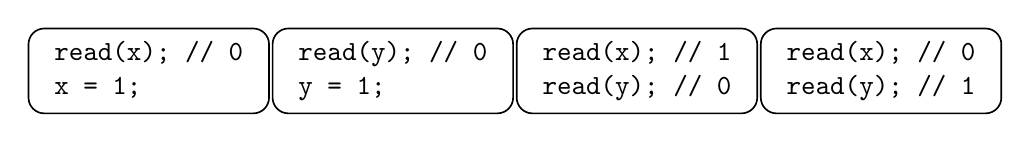
\begin{tikzpicture}[->,>=stealth',shorten >=1pt,auto,node distance=3cm,
   semithick, transform shape]
   % \node[draw, rounded corners=2mm] (t1) at (0, 0) {\begin{tabular}{l} \texttt{x = 1;} \\ \texttt{y = 1;}\end{tabular}};
   \node[draw, rounded corners=2mm] (t2) at (-1.7, -1.5) {\begin{tabular}{l} \texttt{read(x); // 0} \\ \texttt{x = 1;} \end{tabular}};
  \node[draw, rounded corners=2mm] (t3) at (1.4, -1.5) {\begin{tabular}{l} \texttt{read(y); // 0} \\ \texttt{y = 1;} \end{tabular}};
  \node[draw, rounded corners=2mm] (t4) at (4.5, -1.5) {\begin{tabular}{l} \texttt{read(x); // 1} \\ \texttt{read(y); // 0} \end{tabular}};
  \node[draw, rounded corners=2mm] (t5) at (7.6, -1.5) {\begin{tabular}{l} \texttt{read(x); // 0} \\ \texttt{read(y); // 1} \end{tabular}};
  % \node[draw, rounded corners=2mm] (t3) at (1.5, 0) {\begin{tabular}{l} \texttt{read(x); // 2} \\ \texttt{read(y); // 1} \end{tabular}};
  % \path (t1) edge node {} (t3);
  % \path (t2) edge node {$\so$} (t3);
  % \path (t1) edge node {} (t2);
  % \path (t3_1) edge node {$\po$} (t3_2);
  \end{tikzpicture}  
  }
   \caption{Long fork}
   \label{pre_red_example:1}
  \end{subfigure}
%  \hspace{.5cm}
  \begin{subfigure}{.49\textwidth}
  \resizebox{\textwidth}{!}{
  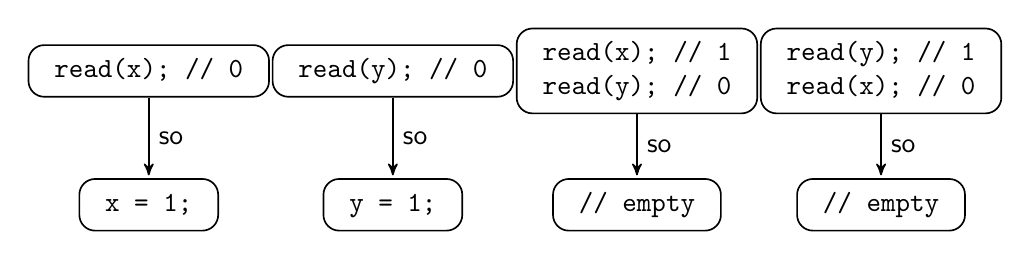
\begin{tikzpicture}[->,>=stealth',shorten >=1pt,auto,node distance=3cm,
   semithick, transform shape]
   % \node[draw, rounded corners=2mm] (t1) at (0, 0) {\begin{tabular}{l} \texttt{x = 1;} \\ \texttt{y = 1;}\end{tabular}};
   \node[draw, rounded corners=2mm] (t2r) at (-1.7, -1.5) {\begin{tabular}{l} \texttt{read(x); // 0} \end{tabular}};
   \node[draw, rounded corners=2mm] (t2w) at (-1.7, -3.2) {\begin{tabular}{l} \texttt{x = 1;} \end{tabular}};
   \node[draw, rounded corners=2mm] (t3r) at (1.4, -1.5) {\begin{tabular}{l} \texttt{read(y); // 0} \end{tabular}};
  \node[draw, rounded corners=2mm] (t3w) at (1.4, -3.2) {\begin{tabular}{l} \texttt{y = 1;} \end{tabular}};
  \node[draw, rounded corners=2mm] (t4r) at (4.5, -1.5) {\begin{tabular}{l} \texttt{read(x); // 1} \\ \texttt{read(y); // 0} \end{tabular}};
  \node[draw, rounded corners=2mm] (t5r) at (7.6, -1.5) {\begin{tabular}{l} \texttt{read(y); // 1} \\ \texttt{read(x); // 0} \end{tabular}}; 
  \node[draw, rounded corners=2mm] (t4w) at (4.5, -3.2) {\begin{tabular}{l} \texttt{// empty} \end{tabular}};
   \node[draw, rounded corners=2mm] (t5w) at (7.6, -3.2) {\begin{tabular}{l} \texttt{// empty} \end{tabular}};
  % \node[draw, rounded corners=2mm] (t3) at (1.5, 0) {\begin{tabular}{l} \texttt{read(x); // 2} \\ \texttt{read(y); // 1} \end{tabular}};
  \path (t2r) edge node {$\so$} (t2w);
  \path (t3r) edge node {$\so$} (t3w);
  \path (t4r) edge node {$\so$} (t4w);
  \path (t5r) edge node {$\so$} (t5w);
  % \path (t2) edge node {$\so$} (t3);
  % \path (t1) edge node {} (t2);
  % \path (t3_1) edge node {$\po$} (t3_2);
  \end{tikzpicture}  
  }
   \caption{Long fork (transformed)}
   \label{pre_red_example:2}
  \end{subfigure}

\vspace{3mm}
  \begin{subfigure}{.26\textwidth}
  \resizebox{\textwidth}{!}{
  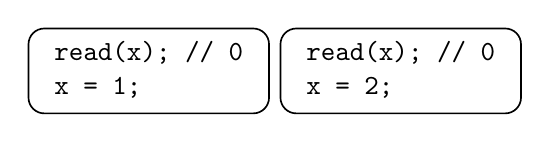
\begin{tikzpicture}[->,>=stealth',shorten >=1pt,auto,node distance=3cm,
   semithick, transform shape]
   % \node[draw, rounded corners=2mm] (t1) at (0, 1.2) {\begin{tabular}{l} \texttt{x = 1;} \end{tabular}};
   \node[draw, rounded corners=2mm] (t2) at (-1.6, 0) {\begin{tabular}{l} \texttt{read(x); // 0} \\ \texttt{x = 1;} \end{tabular}};
   \node[draw, rounded corners=2mm] (t3) at (1.6, 0) {\begin{tabular}{l} \texttt{read(x); // 0} \\ \texttt{x = 2;} \end{tabular}};
   % \node[draw, rounded corners=2mm] (t3) at (0, -2.4) {\begin{tabular}{l} \texttt{read(x); // 2} \end{tabular}};
  % \node[draw, rounded corners=2mm] (t3) at (1.7, -1.5) {\begin{tabular}{l} \texttt{read(y); // 1} \\ \texttt{y = 2;} \end{tabular}};
  % \node[draw, rounded corners=2mm] (t3) at (1.5, 0) {\begin{tabular}{l} \texttt{read(x); // 2} \\ \texttt{read(y); // 1} \end{tabular}};
  % \path (t1) edge node {} (t3);
  % \path (t2) edge node {$\co$} (t3);
  % \path (t1) edge node {} (t2); 
  % \path (t3_1) edge node {$\po$} (t3_2);
  \end{tikzpicture}  
  }
   \caption{Lost update}
   \label{pre_red_example:3}
  \end{subfigure}
  \hspace{2cm}
  \begin{subfigure}{.32\textwidth}
  \resizebox{.75\textwidth}{!}{
  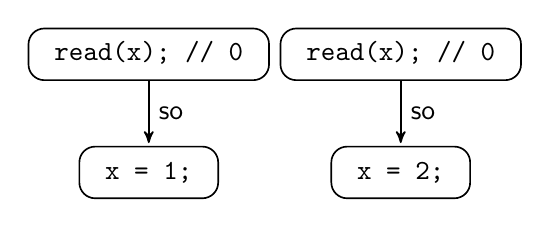
\begin{tikzpicture}[->,>=stealth',shorten >=1pt,auto,node distance=3cm,
   semithick, transform shape]
   % \node[draw, rounded corners=2mm] (t1) at (0, 1.2) {\begin{tabular}{l} \texttt{x = 1;} \end{tabular}};
   \node[draw, rounded corners=2mm] (t2r) at (0, 0) {\begin{tabular}{l} \texttt{read(x); // 0} \end{tabular}};
   \node[draw, rounded corners=2mm] (t2w) at (0, -1.5) {\begin{tabular}{l}  \texttt{x = 1;} \end{tabular}};
   \node[draw, rounded corners=2mm] (t3r) at (3.2, 0) {\begin{tabular}{l} \texttt{read(x); // 0} \end{tabular}};
   \node[draw, rounded corners=2mm] (t3w) at (3.2, -1.5) {\begin{tabular}{l} \texttt{x = 2;} \end{tabular}};
   % \node[draw, rounded corners=2mm] (t3) at (0, -2.4) {\begin{tabular}{l} \texttt{read(x); // 2} \end{tabular}};
  % \node[draw, rounded corners=2mm] (t3) at (1.7, -1.5) {\begin{tabular}{l} \texttt{read(y); // 1} \\ \texttt{y = 2;} \end{tabular}};
  % \node[draw, rounded corners=2mm] (t3) at (1.5, 0) {\begin{tabular}{l} \texttt{read(x); // 2} \\ \texttt{read(y); // 1} \end{tabular}};
  % \path (t1) edge node {} (t3);
  % \path (t2) edge node {$\co$} (t3);
  % \path (t1) edge node {} (t2); 
  % \path (t3_1) edge node {$\po$} (t3_2);
  \path (t2r) edge node {$\so$} (t2w);
  \path (t3r) edge node {$\so$} (t3w);
  \end{tikzpicture}  
  }
   \caption{Lost update (transformed)}
   \label{pre_red_example:4}
  \end{subfigure}
  \vspace{-3mm}
  \caption{Reducing PC to SER. Initially, the value of every variable is 0.}
  \label{pre_red_example}
  \vspace{-3mm}
\end{figure}

The following lemma is a straightforward consequence of the definitions. % (see Appendix~\ref{app:pc_red}).

\begin{lemma}\label{lem:pc_width}
The histories $\hist$ and $\hist_{R|W}$ have the same width.
\end{lemma}

Next, we show that $\hist_{R|W}$ is serializable if $\hist$ is prefix consistent. Formally, we show that
 \begin{align*}
  \forall \co.\ \exists \co'.\ \tup{\hist, \co} \models \axpre \Rightarrow \tup{\hist_{R|W}, \co'} \models \axser 
 \end{align*}
%\begin{theorem}
% There is a polynomial time reduction from prefix consistency verification problem to serialization verification problem - without increasing the width of the history.
%\end{theorem}
%
%
%Now we claim, $\hist$ is prefix consistent if and only if $\hist_{R|W}$ is serializable.
%
%\begin{proof}
% First we will prove, if $\hist$ is prefix consistent, then $\hist_{R|W}$ is serializable. Formally we are trying to prove,
% 
% \begin{align}
%  \forall \co, \exists \co' \tup{\hist, \co} \models \axpre \Rightarrow \tup{\hist_{R|W}, \co'} \models \axser \label{pre_leftright}
% \end{align}
%
% Consider a total order $\co$ for $\hist$ which satisfies prefix consistency. We will show there exists a $\co'$ for $\hist_{R|W}$ which satisfies serialization. To find such $\co'$, first we construct a partial order $\co'_1$ on $T'$ and then try to extend $\co'_1$ to $\co'$.
Thus, let $\co$ be a commit (total) order on transactions of $\hist$ which together with $\hist$ satisfies the prefix consistency axiom. We define two \emph{partial} commit orders $\co'_1$ and $\co'_2$, $\co'_2$ a strengthening of $\co'_1$, which we prove that they are acyclic and that any linearization $\co'$ of $\co'_2$ is a valid witness for $\hist_{R|W}$ satisfying serializability.

Thus, let $\co'_1$ be a \emph{partial} commit order on transactions of $\hist_{R|W}$ defined as follows:
 \begin{align*}
  \co'_1 = \{\tup{R_{\tr}, W_{\tr}} | \tr \in T\} \cup \{\tup{W_{\tr_1}, W_{\tr_2}} | \tup{\tr_1, \tr_2} \in \co\}\ \cup \{\tup{W_{\tr_1},R_{\tr_2}} | \tup{\tr_1, \tr_2} \in \wro \cup \so\} 
 \end{align*}
 
We show that if $\co'_1$ were to be cyclic, then it contains a minimal cycle with one read transaction, and at least one but at most two write transactions. Then, we show that such cycles cannot exist. 

 \begin{lemma}\label{lem:co1}
The relation $\co'_1$ is acyclic.
\end{lemma}
% \begin{proof}
% Now we will show $\co'_1$ is acyclic. To do that, first we show few properties of a minimal cycle in $\co'_1$ to ease our proofs. 
 \textsc{Proof.} We first show that if $\co'_1$ were to be cyclic, then it contains a minimal cycle with one read transaction, and at least one but at most two write transactions. Then, we show that such cycles cannot exist. 
Therefore, let us assume that $\co'_1$ is cyclic. Then,
%\vspace{-4mm}
  \begin{figure}
 \centering
  \begin{subfigure}{.26\textwidth}
   \resizebox{\textwidth}{!}{
    \begin{tikzpicture}[->,>=stealth',shorten >=1pt,auto,node distance=4cm,
      semithick, transform shape]
     \node[transaction state] at (0,0)       (t_1)           {$W_{\tr_1}$};
     \node[transaction state] at (2,0)       (t_2)           {$W_{\tr_2}$};
     \path (t_1) edge[dashed, bend left=90] node {$\co'^+_1$} (t_2);
     \path (t_2) edge[dashed, color=red, bend left=90] node {$\co'^+_1$} (t_1);
     \path (t_1) edge[color=red] node[below] {$\co'_1$} (t_2);
    \end{tikzpicture}  
   }
   \caption{$\tup{W_{\tr_1}, W_{\tr_2}} \in \co'_1$}
   \label{ww_consecutive:a}
  \end{subfigure}
  \hspace{1mm}
  \begin{subfigure}{.25\textwidth}
   \resizebox{\textwidth}{!}{
    \begin{tikzpicture}[->,>=stealth',shorten >=1pt,auto,node distance=4cm,
      semithick, transform shape]
     \node[transaction state] at (0,0)       (t_1)           {$W_{\tr_1}$};
     \node[transaction state] at (2,0)       (t_2)           {$W_{\tr_2}$};
     \path (t_1) edge[dashed, color=blue, bend left=90] node {$\co'^+_1$} (t_2);
     \path (t_2) edge[dashed, bend left=90] node {$\co'^+_1$} (t_1);
     \path (t_2) edge[color=blue] node[above] {$\co'_1$} (t_1);
    \end{tikzpicture}  
   }
   \caption{$\tup{W_{\tr_2}, W_{\tr_1}} \in \co'_1$}
   \label{ww_consecutive:b}
  \end{subfigure}
  \vspace{-3mm}
  \caption{Cycles with non-consecutive write transactions.}
  \label{ww_consecutive}
  \vspace{-5mm}
 \end{figure} 
 \begin{itemize}
  \item Since $\tup{W_{\tr_1}, W_{\tr_2}} \in \co'_1$ implies $\tup{\tr_1, \tr_2} \in \co$, for every $\tr_1$ and $\tr_2$, a cycle in $\co'_1$ cannot contain only write transactions. Otherwise, it will imply a cycle in the original commit order $\co$. Therefore, a cycle in $\co'_1$ must contain at least one read transaction. 
  \item Assume that a cycle in $\co'_1$ contains two write transactions $W_{\tr_1}$ and $W_{\tr_2}$ which are not consecutive, like in Figure~\ref{ww_consecutive}.
%  In figure \ref{ww_consecutive}, we have a minimal cycle in $\co'_1$ in which there are two transactions $W_{\tr_1}$ and $W_{\tr_2}$ which are not consecutive. 
Since either $\tup{W_{\tr_1}, W_{\tr_2}}\in \co'_1$ or $\tup{W_{\tr_1}, W_{\tr_2}}\in \co'_1$, there exists a smaller cycle in $\co'_1$ where these two write transactions are consecutive. If $\tup{W_{\tr_1}, W_{\tr_2}}\in \co'_1$, then $\co'_1$ contains the smaller cycle on the lower part of the original cycle (Figure~\ref{ww_consecutive:a}), and if $\tup{W_{\tr_2}, W_{\tr_1}}\in \co'_1$, then $\co'_1$ contains the cycle on the upper part of the original cycle (Figure~\ref{ww_consecutive:b}). Thus, all the write transactions in a minimal cycle of $\co'_1$ must be consecutive. 
% So all $W_{\_}$ transactions in a minimal cycle in $\co'_1$ must be consecutive.
\end{itemize}

\begin{itemize}
  \item If a minimal cycle were to contain three write transactions, then all of them cannot be consecutive unless they all three form a cycle, which is not possible. So a minimal cycle contains at most two write transactions.
  \item Since $\co'_1$ contains no direct relation between read transactions, it cannot contain a cycle with two consecutive read transactions, or only read transactions.
  %there is no relation of the form $\tup{R_{\_}, R_{\_}}$ in $\co'_1$. So there is no cycle with consecutive $R_{\_}$ transactions.
%  \item All these above properties togerther imply a minimal cycle in $\co'_1$ contains atleast one but atmost two $W_{\_}$ transactions and one $R_{\_}$ transaction.
 \end{itemize}
This shows that a minimal cycle of $\co'_1$ would include a read transaction and a write transaction, and at most one more write transaction. We prove that such cycles are however impossible:
 \begin{itemize}
  \item if the cycle is of size 2, then it contains two transactions $W_{\tr_1}$ and $R_{\tr_2}$ such that $\tup{W_{\tr_1}, R_{\tr_2}}\in\co'_1$ and $\tup{R_{\tr_2}, W_{\tr_1}}\in \co'_1$. Since all the $\tup{R_{\_}, W_{\_}}$ dependencies in $\co'_1$ are of the form $\tup{R_\tr, W_\tr}$, it follows that $\tr_1 = \tr_2$. Then, we have $\tup{W_{\tr_1}, R_{\tr_1}} \in \co'_1$ which implies $\tup{\tr_1, \tr_1} \in \wro \cup \so$, a contradiction.
  \item if the cycle is of size 3, then it contains three transactions $W_{\tr_1}$, $W_{\tr_2}$, and $R_{\tr_3}$ such that $\tup{W_{\tr_1}, W_{\tr_2}}\in \co'_1$,  $\tup{W_{\tr_2}, R_{\tr_3}}\in \co'_1$, and $\tup{R_{\tr_3}, W_{\tr_1}} \in \co'_1$. Using a similar argument as in the previous case, $\tup{R_{\tr_3}, W_{\tr_1}} \in \co'_1$ implies $\tr_3 = \tr_1$. Therefore, $\tup{\tr_1, \tr_2} \in \co$ and $\tup{\tr_2, \tr_1} \in \wro \cup \so$, which contradicts the fact that $\wro \cup \so\subseteq \co$. \hfill $\Box$
  %  satisfies prefix consistency for $\hist$.
 \end{itemize}
% \end{proof}

 
 %Therefore, $\co'_1$ is acyclic. 
%Now we want to remove the choices for which any acyclic extension of $\co'_1$ will violate $\axser$. The extension will be a total order, so if we do not want a relation $\tup{\tr_1, \tr_2}$ in $\co'$, then $\tup{\tr_2, \tr_1}$ must be in it. So we collect all such relations implied by $\co'_1$ in 
 We define a strengthening of $\co'_1$ where intuitively, we add all the dependencies from read transactions $\tr_3$ to write transactions $\tr_2$ that ``overwrite'' values read by $\tr_3$. Formally, $\co'_2= \co'_1\cup\rwo(\co'_1)$ where 
 \begin{align*}
  \rwo(\co'_1) = \{\tup{\tr_3, \tr_2}| \exists \xvar \in \vars{h}.\ \exists \tr_1\in T'.\ \tup{\tr_1,\tr_3} \in \wro[\xvar]', \tup{\tr_1, \tr_2} \in \co'_1, \writeVar{\tr_2}{\xvar} \} 
 \end{align*}
 
 It can be shown that any cycle in $\co'_2$ would correspond to a $\mathsf{Prefix}$ violation in the original history. Therefore,
 
  \begin{figure}[h] %{l}{0.5\textwidth} 
  \centering
  \begin{subfigure}{.26\textwidth}
   \resizebox{\textwidth}{!}{
    \begin{tikzpicture}[->,>=stealth',shorten >=1pt,auto,node distance=4cm,
      semithick, transform shape]
     \node[transaction state] at (0,0)       (t_1)           {$W_{\tr_1}$};
     \node[transaction state] at (2,0)       (t_3)           {$R_{\tr_3}$};
     \node[transaction state, label={above:$\writeVar{ }{\xvar}$}] at (-0.5,1.5) (t_2) {$W_{\tr_2}$};
     \node[transaction state] at (1.5,1.5) (t_4) {$W_{\tr_4}$};
     \path (t_1) edge node {$\wro[\xvar]$} (t_3);
     % \path (t_2) edge[blue] node {$\CO$} (t_1);
     \path (t_2) edge[red] node {$\co'^*_1$} (t_4);
     \path (t_4) edge[red] node {$\co'_1$} (t_3);
     \path (t_1) edge[left] node {$\co'_1$} (t_2);
     \path (t_3) edge[red, right] node[pos=.8,rotate=-30,yshift=2.5mm] {\small{$\rwo(\co'_1)$}} (t_2);
    \end{tikzpicture}
   }
   \caption{}
   \label{pc_p_proof:2a}
  \end{subfigure}
  \hspace{10mm}
  \begin{subfigure}{0.31\textwidth}
   \resizebox{\textwidth}{!}{
    \begin{tikzpicture}[->,>=stealth',shorten >=1pt,auto,node distance=4cm,
      semithick, transform shape]
     \node[transaction state, text=red] at (0,0)       (t_1)           {$\tr_1$};
     \node[transaction state] at (2,0)       (t_3)           {$\tr_3$};
     \node[transaction state, text=red,label={above:\textcolor{red}{$\writeVar{ }{\xvar}$}}] at (-0.5,1.5) (t_2) {$\tr_2$};
     \node[transaction state] at (1.5,1.5) (t_4) {$\tr_4$};
     \path (t_1) edge[red] node {$\wro[\xvar]$} (t_3);
     % \path (t_2) edge[blue] node {$\CO$} (t_1);
     \path (t_2) edge node {$\co^*$} (t_4);
     \path (t_4) edge node {$\wro \cup \so$} (t_3);
     \path (t_1) edge[left] node {$\co$} (t_2);
    \end{tikzpicture}
   }
   \caption{}
   \label{pc_p_proof:2b}
  \end{subfigure}
%   \vspace{-3mm}
  \caption{Cycles in $\co'_2$ correspond to $\axpre$ violations: (a) Minimal cycle in $\co'_2$, (b) $\axpre$ violation in $\tup{\hist, \co}$.}
  \label{pc_p_proof:2}
%   \vspace{-2.5mm}
 \end{figure}

 
 %\vspace{-1mm}
 \begin{lemma}\label{lem:co2}
 The relation $\co'_2$ is acyclic.
 \end{lemma}
 \begin{proof}
 Assume that $\co'_2$ is cyclic. Any minimal cycle in $\co'_2$ still satisfies the properties of minimal cycles of $\co'_1$ proved in Lemma~\ref{lem:co1} (because all write transactions are still totally ordered and $\co'_2$ doesn't relate directly read transactions). 
 %- $\co'_2$ has relations of the form $\tup{R_{\_}, W_{\_}}$. 
 So, a minimal cycle in $\co'_2$ contains a read transaction and a write transaction, and at most one more write transaction.
 
 Since $\co'_1$ is acyclic, a cycle in $\co'_2$, and in particular a minimal one, must  necessarily contain a dependency from $\rwo(\co'_1)$. Note that a minimal cycle cannot contain two such dependencies since this would imply that it contains two non-consecutive write transactions. 
%  $\co'_1$ was acyclic. All the relations in $\co'_2$ are of the form $\tup{R_{\_}, W_{\_}}$. If $(\co'_1 \cup \co'_2)$ has a cycle, then the cycle must contain an relation from $\co'_2$. But two $\tup{R_{\_}, W_{\_}}$ in a cycle implies, two non-consecutive $W_{\_}$ in a cycle. So a simple cycle in $(\co'_1 \cup \co'_2)$ would contain only one relation of the form $\tup{R_{\_}, W_{\_}}$.
% 
The red edges in Figure~\ref{pc_p_proof:2a} show a minimal cycle of $\co'_2$ satisfying all the properties mentioned above. This cycle contains a dependency $\tup{R_{\tr_3}, W_{\tr_2}}\in \rwo(\co'_1)$ which implies the existence of a write transaction $W_{\tr_1}$ in $\hist_{R|W}$ s.t. $\tup{W_{\tr_1}, R_{\tr_3}} \in \wro[\xvar]'$ and $\tup{W_{\tr_1}, W_{\tr_2}} \in \co'_1$ and $W_{\tr_1}, W_{\tr_2}$ write on $\xvar$ (these dependencies are represented by the black edges in Figure~\ref{pc_p_proof:2a}). The relations between these transactions of $\hist_{R|W}$ imply that the corresponding transactions of $\hist$ are related as shown in Figure~\ref{pc_p_proof:2b}: $\tup{W_{\tr_1}, W_{\tr_2}} \in \co'_1$ and $\tup{W_{\tr_2}, W_{\tr_4}} \in \co'^*_1$ imply $\tup{\tr_1, \tr_2} \in \co$ and $\tup{\tr_2, \tr_4} \in \co^*$, respectively, $\tup{W_{\tr_1}, W_{\tr_3}} \in \wro[\xvar]'$ implies $\tup{\tr_1, \tr_3} \in \wro[\xvar]$, and $\tup{W_{\tr_4}, R_{\tr_3}} \in \co'_1$ implies $\tup{\tr_4, \tr_3} \in \wro \cup \so$. This implies that $\tup{\hist,\co}$ doesn't satisfy the $\axpre$ axiom, a contradiction. %\hfill $\Box$
%But to satisfy $\axpre$, $\tup{\tr_2, \tr_1}$ should have been in $\co$, not $\tup{\tr_1, \tr_2}$ - which is a contradiction.
\end{proof}
 
 

 \begin{lemma}\label{lem:pc1:app}
If a history $\hist$ satisfies prefix consistency, then $\hist_{R|W}$ is serializable.
\end{lemma}
 \begin{proof}
% So $\co'_1 \cup \co'_2$ is acyclic. We take $\co'$ to be any topological order of $\co'_1 \cup \co'_2$. 
 Let $\co'$ be any total order consistent with $\co'_2$. Assume by contradiction that $\tup{\hist_{R|W},\co'}$ doesn't satisfy $\axser$. Then, there exist $\tr'_1, \tr'_2, \tr'_3 \in T'$ such that $\tup{\tr'_1, \tr'_2}, \tup{\tr'_2, \tr'_3} \in \co'$ and $\tr'_1, \tr'_2$ write on some variable $\xvar$ and $\tup{\tr'_1, \tr'_3} \in \wro[\xvar]'$. But then $\tr'_1, \tr'_2$ are write transactions and $\co'_1$ must contain $\tup{\tr'_1, \tr'_2}$. Therefore, $\rwo(\co'_1)$ and $\co'_2$ should contain $\tup{\tr'_3, \tr'_2}$, a contradiction with $\co'$ being consistent with $\co'_2$.
%  we must have added $\tup{\tr'_3, \tr'_2} \in \co'_2$. So $\tup{\tr'_2, \tr'_3}$ can not be in $\co'$. Therefore, $\co'$ must satisfy $\axser$ and proves our claim in predicate (\ref{pre_leftright}).
 \end{proof}

 
 Finally, it can be proved that any linearization $\co'$ of $\co'_2$ satisfies $\mathsf{Serializability}$ (together with $\hist_{R|W}$). Moreover, it can also be shown that the serializability of $\hist_{R|W}$ implies that $\hist$ satisfies PC. Therefore,

\begin{theorem}\label{th:pc}
A history $\hist$ satisfies prefix consistency iff $\hist_{R|W}$ is serializable.
\end{theorem}
\textsc{Proof.}
The ``only-if'' direction is proven by Lemma~\ref{lem:pc1:app}. For the reverse, we show that 
 % Now we will prove, if $\hist_{R|W}$ is serializable, then $\hist$ is prefix consistent. Formally we are trying to prove,
\begin{align*}
\forall \co'.\ \exists \co.\ \tup{\hist_{R|W}, \co'} \models \axser \Rightarrow \tup{\hist, \co} \models \axpre %\label{pre_rightleft}
\end{align*}

%\noindent
%$\forall \co'.\ \exists \co.\ \tup{\hist_{R|W}, \co'} \models \axser $
%
%\hspace{3cm}
%$\Rightarrow \tup{\hist, \co} \models \axpre$ %\label{pre_rightleft}
 
  \begin{figure}[t] %{l}{0.53\textwidth} 
  \centering
  \begin{subfigure}{.31\textwidth}
   \resizebox{\textwidth}{!}{
    \begin{tikzpicture}[->,>=stealth',shorten >=1pt,auto,node distance=4cm,
      semithick, transform shape]
     \node[transaction state, text=red] at (0,0)       (t_1)           {$\tr_1$};
     \node[transaction state] at (2,0)       (t_3)           {$\tr_3$};
     \node[transaction state, text=red,label={above:\textcolor{red}{$\writeVar{ }{\xvar}$}}] at (-0.5,1.5) (t_2) {$\tr_2$};
     \node[transaction state] at (1.5,1.5) (t_4) {$\tr_4$};
     \path (t_1) edge[red] node {$\wro[\xvar]$} (t_3);
     % \path (t_2) edge[blue] node {$\CO$} (t_1);
     \path (t_2) edge node {$\co^*$} (t_4);
     \path (t_4) edge node {$\wro \cup \so$} (t_3);
     \path (t_1) edge[left] node {$\co$} (t_2);
    \end{tikzpicture}
   }
   \caption{}
   \label{pc_p_proof:3a}
  \end{subfigure}
  \hspace{10mm}
  \begin{subfigure}{0.31\textwidth}
   \resizebox{\textwidth}{!}{
    \begin{tikzpicture}[->,>=stealth',shorten >=1pt,auto,node distance=4cm,
      semithick, transform shape]
     \node[transaction state] at (0,0)       (t_1)           {$W_{\tr_1}$};
     \node[transaction state] at (2,0)       (t_3)           {$R_{\tr_3}$};
     \node[transaction state, label={above:\textcolor{red}{$\writeVar{ }{\xvar}$}}] at (-0.5,1.5) (t_2) {$W_{\tr_2}$};
     \node[transaction state] at (1.5,1.5) (t_4) {$W{\tr_4}$};
     \path (t_1) edge node[near start] {$\wro[\xvar]'$} (t_3);
     % \path (t_2) edge[blue] node {$\CO$} (t_1);
     \path (t_2) edge[red] node {$\co'^*$} (t_4);
     \path (t_4) edge[red] node {$\wro' \cup \so'$} (t_3);
     \path (t_1) edge[left] node {$\co'$} (t_2);
     \path (t_3) edge[red,above right] node {$\co'$} (t_2);
    \end{tikzpicture}
   }
   \caption{}
   \label{pc_p_proof:3b}
  \end{subfigure}
  
  \caption{$\axpre$ violations correspond to cycles in $\co'$: (a) $\axpre$ violation in $\tup{\hist, \co}$, (b) Cycle in $\co'$.}
  \label{pc_p_proof:3}
 \end{figure}
 
 Thus, let $\co'$ be a commit (total) order on transactions of $\hist_{R|W}$ which together with $\hist_{R|W}$ satisfies the serializability axiom.
 % Consider a total order $\co'$ for $\hist_{R|W}$ which satisfies serialization. We will show there exists a $\co$ for $h$ which satisfies prefix consistency. 
 Let $\co$ be a commit order on transactions of $\hist$ defined by 
 $\co = \{\tup{\tr_1, \tr_2} | \tup{W_{\tr_1}, W_{\tr_2}} \in \co'\}$ ($\co$ is clearly a total order). If $\co$ were not to be consistent with $\wro \cup \so$, then there would exist transactions $\tr_1$ and $\tr_2$ such that  $\tup{\tr_1, \tr_2} \in \wro \cup \so$ and $\tup{\tr_2, \tr_1} \in \co$, which would imply that $\tup{W_{\tr_1}, R_{\tr_2}} , \tup{R_{\tr_2}, W_{\tr_2}} \in \wro \cup \so$ and $\tup{W_{\tr_2}, W_{\tr_1}} \in \co'$, which violates the acylicity of $\co'$. We show that $\tup{\hist, \co}$ satisfies $\axpre$. Assume by contradiction that there exists a $\axpre$ violation between $\tr_1$, $\tr_2$, $\tr_3$, $\tr_4$ (shown in Figure \ref{pc_p_proof:3a}), i.e., for some $\xvar \in \vars{\hist}$, $\tup{\tr_1, \tr_3} \in \wro[\xvar]$ and $\writeVar{\tr_2}{\xvar}$, $\tup{\tr_1, \tr_2} \in \co$, $\tup{\tr_2, \tr_4} \in \co^*$ and $\tup{\tr_4, \tr_3} \in \wro \cup \so$. Then, the corresponding transactions $W_{\tr_1}, W_{\tr_2}, W_{\tr_4}, R_{\tr_3}$ in $\hist_{R|W}$ would be related as follows: 
$\tup{W_{\tr_1}, W_{\tr_2}} \in \co'$ and $\tup{W_{\tr_1}, R_{\tr_3}} \in \wro[\xvar]'$ because $\tup{\tr_1, \tr_3} \in \wro[\xvar]$ and $\tup{\tr_1, \tr_2} \in \co$.
        Since $\co'$ satisfies $\axser$, then $\tup{R_{\tr_3}, W_{\tr_2}} \in \co'$.
        But $\tup{\tr_2, \tr_4} \in \co^*$ and $\tup{\tr_4, \tr_3} \in \wro \cup \so$ imply that $\tup{W_{\tr_2}, W_{\tr_4}} \in \co'^*$ and $\tup{W_{\tr_4}, R_{\tr_3}} \in \wro' \cup \so'$, which show that $\co'$ is cyclic (the red cycle in Figure \ref{pc_p_proof:3b}), a contradiction. \hfill $\Box$

 
 
 
 
Since the history $\hist_{R|W}$ can be constructed in linear time, Lemma~\ref{lem:pc_width}, Theorem~\ref{th:pc}, and Corollary~\ref{cor:ser} imply the following result.
 
 \begin{corollary}\label{cor:pc}
 
For an arbitrary but fixed constant $k\in\mathbb{N}$, the problem of checking prefix consistency for histories of width at most $k$ is polynomial time.
 \end{corollary}
 
%\end{proof}


%!TEX root = Thesis.tex



\subsection{Reducing Snapshot Isolation to Serializability}\label{ssec:si}

We extend the reduction of prefix consistency to serializability to the case of snapshot isolation. Compared to prefix consistency, snapshot isolation disallows transactions that read the same snapshot of the database to commit together if they write on a common variable (stated by the $\mathsf{Conflict}$ axiom). More precisely, for any pair of transactions $\tr_1$ and $\tr_2$ writing to a common variable, $\tr_1$ must observe the effects of $\tr_2$ or vice-versa. 
%when one of these transactions reads a variable written by the other one. 
We refine the definition of $\hist_{R|W}$ such that any ``serialization'' (i.e.., commit order satisfying $\mathsf{Serializability}$) disallows that the read transactions corresponding to two such transactions are ordered both before their write counterparts. We do this by introducing auxiliary variables that are read or written by these transactions. For instance, 
Figure~\ref{si_red_example} shows this transformation on the two histories in Figure~\ref{si_red_example:1} and Figure~\ref{si_red_example:3}, which represent the anomalies known as ``lost update'' and ``write skew'', respectively. The former is not admitted by SI while the latter is admitted. Concerning ``lost update'', the read counterpart of the transaction on the left writes to a variable {\tt x12} that is read by its write counterpart, but also written by the write counterpart of the other transaction. This forbids that the latter is serialized in between the read and write counterparts of the transaction on the left. A similar scenario is imposed on the transaction on the right, which makes that the transformed history is not serializable. Concerning the ``write skew'' anomaly, the transformed history is exactly as for the PC reduction since the two transactions don't write on a common variable. It is clearly serializable.

%\begin{theorem}
% There is a polynomial time reduction from snapshot isolation verification problem to serialization verification problem - without increasing the width of the history.
%\end{theorem}

For a history $\hist = \tup{T, \wro, \so}$, the history $\hist_{R|W}^c = \tup{T', \wro', \so'}$ is defined as $\hist_{R|W}$ with the following additional construction: for every two transactions $\tr_1$ and $\tr_2 \in T$ that write on a common variable,
% and $\hist_{R|W} = \tup{T', \wro', \so'}$, we define the history $\hist_{R|W}^c = \tup{T', \wro'', \so'}$ where 
\begin{itemize}
%\item for every variable $\xvar$ in the original history $\hist$, i.e., $\wro''[\xvar]=\wro'[\xvar]$,
\item $R_{\tr_1}$ and $W_{\tr_2}$ (resp., $R_{\tr_2}$ and $W_{\tr_1}$) write on a variable $\xvar_{1,2}$ (resp., $\xvar_{2,1}$),
\item the write transaction of $\tr_i$ reads $\xvar_{i,j}$ from the read transaction of $\tr_i$, for all $i\neq j\in\{1,2\}$, i.e., $\wro[\xvar_{1,2}]= \{\tup{R_{\tr_1}, W_{\tr_1}}\}$ and $\wro[\xvar_{2,1}]= \{\tup{R_{\tr_2}, W_{\tr_2}}\}$.
\end{itemize}

\begin{figure}
  
  
    \begin{subfigure}{.24\textwidth}
    \resizebox{\textwidth}{!}{
    \begin{tikzpicture}[->,>=stealth',shorten >=1pt,auto,node distance=3cm,
     semithick, transform shape]
     % \node[draw, rounded corners=2mm] (t1) at (0, 1.2) {\begin{tabular}{l} \texttt{x = 1;} \end{tabular}};
     \node[draw, rounded corners=2mm] (t2) at (-1.6, 0) {\begin{tabular}{l} \texttt{read(x); // 0} \\ \texttt{x = 1;} \end{tabular}};
     \node[draw, rounded corners=2mm] (t3) at (1.6, 0) {\begin{tabular}{l} \texttt{read(x); // 0} \\ \texttt{x = 2;} \end{tabular}};
     % \node[draw, rounded corners=2mm] (t3) at (0, -2.4) {\begin{tabular}{l} \texttt{read(x); // 2} \end{tabular}};
    % \node[draw, rounded corners=2mm] (t3) at (1.7, -1.5) {\begin{tabular}{l} \texttt{read(y); // 1} \\ \texttt{y = 2;} \end{tabular}};
    % \node[draw, rounded corners=2mm] (t3) at (1.5, 0) {\begin{tabular}{l} \texttt{read(x); // 2} \\ \texttt{read(y); // 1} \end{tabular}};
    % \path (t1) edge node {} (t3);
    % \path (t2) edge node {$\co$} (t3);
    % \path (t1) edge node {} (t2); 
    % \path (t3_1) edge node {$\po$} (t3_2);
    \end{tikzpicture}  
    }
     \caption{Lost update}
     \label{si_red_example:1}
    \end{subfigure}
%    \hspace{3mm}
    \begin{subfigure}{.24\textwidth}
    \resizebox{\textwidth}{!}{
    \begin{tikzpicture}[->,>=stealth',shorten >=1pt,auto,node distance=3cm,
     semithick, transform shape]
     % \node[draw, rounded corners=2mm] (t1) at (0, 1.2) {\begin{tabular}{l} \texttt{x = 1;} \end{tabular}};
     \node[draw, rounded corners=2mm] (t2r) at (-1.8, .9) {\begin{tabular}{l} \texttt{read(x); // 0} \\ \texttt{x12 = 1;} \end{tabular}};
     \node[draw, rounded corners=2mm] (t2w) at (-1.8, -.9) {\begin{tabular}{l}  \texttt{x = 1;}  \\ \texttt{read(x12); // 1} \\ \texttt{x21 = 2;} \end{tabular}};
     \node[draw, rounded corners=2mm] (t3r) at (1.8, .9) {\begin{tabular}{l} \texttt{read(x); // 0} \\ \texttt{x21 = 1;} \end{tabular}};
     \node[draw, rounded corners=2mm] (t3w) at (1.8, -.9) {\begin{tabular}{l} \texttt{x = 2;}  \\ \texttt{read(x21); // 1} \\ \texttt{x12 = 2;}\end{tabular}};
     % \node[draw, rounded corners=2mm] (t3) at (0, -2.4) {\begin{tabular}{l} \texttt{read(x); // 2} \end{tabular}};
    % \node[draw, rounded corners=2mm] (t3) at (1.7, -1.5) {\begin{tabular}{l} \texttt{read(y); // 1} \\ \texttt{y = 2;} \end{tabular}};
    % \node[draw, rounded corners=2mm] (t3) at (1.5, 0) {\begin{tabular}{l} \texttt{read(x); // 2} \\ \texttt{read(y); // 1} \end{tabular}};
    % \path (t1) edge node {} (t3);
    % \path (t2) edge node {$\co$} (t3);
    % \path (t1) edge node {} (t2); 
    % \path (t3_1) edge node {$\po$} (t3_2);
    \path (t2r) edge node {$\so$} (t2w);
    \path (t3r) edge node {$\so$} (t3w);
    \end{tikzpicture}  
    }
     \caption{Lost update (transformed)}
     \label{si_red_example:2}
    \end{subfigure}
%    \hspace{3mm}
  \begin{subfigure}{.24\textwidth}
  \resizebox{\textwidth}{!}{
  \begin{tikzpicture}[->,>=stealth',shorten >=1pt,auto,node distance=3cm,
   semithick, transform shape]
   % \node[draw, rounded corners=2mm] (t1) at (0, 0) {\begin{tabular}{l} \texttt{x = 1;} \\ \texttt{y = 1;}\end{tabular}};
   \node[draw, rounded corners=2mm] (t2) at (-1.6, -1.5) {\begin{tabular}{l} \texttt{read(x); // 0} \\ \texttt{read(y); // 0} \\ \texttt{x = 1;} \end{tabular}};
   \node[draw, rounded corners=2mm] (t3) at (1.6, -1.5) {\begin{tabular}{l} \texttt{read(x); // 0} \\ \texttt{read(y); // 0} \\ \texttt{y = 1;} \end{tabular}};
  % \node[draw, rounded corners=2mm] (t3) at (1.7, -1.5) {\begin{tabular}{l} \texttt{read(y); // 1} \\ \texttt{y = 2;} \end{tabular}};
  % \node[draw, rounded corners=2mm] (t3) at (1.5, 0) {\begin{tabular}{l} \texttt{read(x); // 2} \\ \texttt{read(y); // 1} \end{tabular}};
  % \path (t1) edge node {} (t3);
  % \path (t2) edge node {$\so$} (t3);
  % \path (t1) edge node {} (t2);
  % \path (t3_1) edge node {$\po$} (t3_2);
  \end{tikzpicture}  
  }
   \caption{Write skew}
   \label{si_red_example:3}
  \end{subfigure}
%  \hspace{3mm}
  \begin{subfigure}{.24\textwidth}
  \resizebox{\textwidth}{!}{
  \begin{tikzpicture}[->,>=stealth',shorten >=1pt,auto,node distance=3cm,
   semithick, transform shape]
   % \node[draw, rounded corners=2mm] (t1) at (0, 0) {\begin{tabular}{l} \texttt{x = 1;} \\ \texttt{y = 1;}\end{tabular}};
   \node[draw, rounded corners=2mm] (t2r) at (-1.6, 0) {\begin{tabular}{l} \texttt{read(x); // 0} \\ \texttt{read(y); // 0} \end{tabular}};
   \node[draw, rounded corners=2mm] (t2w) at (-1.6, -1.3) {\begin{tabular}{l} \texttt{x = 1;} \end{tabular}};
   \node[draw, rounded corners=2mm] (t3r) at (1.6, 0) {\begin{tabular}{l} \texttt{read(x); // 0} \\ \texttt{read(y); // 0} \end{tabular}};
   \node[draw, rounded corners=2mm] (t3w) at (1.6, -1.3) {\begin{tabular}{l} \texttt{y = 1;} \end{tabular}};
  % \node[draw, rounded corners=2mm] (t3) at (1.7, -1.5) {\begin{tabular}{l} \texttt{read(y); // 1} \\ \texttt{y = 2;} \end{tabular}};
  % \node[draw, rounded corners=2mm] (t3) at (1.5, 0) {\begin{tabular}{l} \texttt{read(x); // 2} \\ \texttt{read(y); // 1} \end{tabular}};
  % \path (t1) edge node {} (t3);
  % \path (t2) edge node {$\so$} (t3);
  % \path (t1) edge node {} (t2);
  % \path (t3_1) edge node {$\po$} (t3_2);
  \path (t2r) edge node {$\so$} (t2w);
  \path (t3r) edge node {$\so$} (t3w);
  \end{tikzpicture}  
  }
   \caption{Write skew (transformed)}
   \label{si_red_example:4}
  \end{subfigure}
%   \vspace{-3mm}
  \caption{Reducing SI to SER.}
  \label{si_red_example}
%   \vspace{-3mm}
\end{figure}


%we create a new history $\hist' = \tup{\Tr', \wro', \so'}$,
%\begin{itemize}
% \item $\Tr' = \{R_\tr | \tr \in \Tr\} \cup \{W_\tr | \tr \in \Tr\}$
% \item $W_{\tr}$ writes on $\xvar$ if $\tr$ writes on $\xvar$.
% \item For each pair of unique transactions $(\tr_1, \tr_2) \in \Tr \times \Tr$, if $\tr_1, \tr_2$ write on overlapping variables, then $W_{\tr_1}, R_{\tr_2}$ write on a new variable $\xvar_{\tr_2\tr_1}$ $W_{\tr_2}$ reads it from $R_{\tr_2}$. $\wro[\xvar_{\tr_2\tr_1}] = \{\tup{R_{\tr_2}, W_{\tr_1}}\}$.
% \item $\wro[\xvar]' = \{\tup{W_{\tr_1}, R_{\tr_2}} | \tup{\tr_1, \tr_2} \in \wro[\xvar]\}$
% \item $\so' = \{\tup{R_\tr, W_\tr} | \tr \in \Tr\} \cup$
%       
%       $\{\tup{W_{\tr_1}, W_{\tr_2}}, \tup{W_{\tr_1}, R_{\tr_2}}, \tup{R_{\tr_1}, W_{\tr_2}}, \tup{R_{\tr_1}, R_{\tr_2}} | \tup{\tr_1,\tr_2} \in \so \}$ 
%       
%\end{itemize}
%
%Constructing $\Tr', \wro[\xvar]', \so'$ can be done in similar way from prefix consistency reduction. Here, we just need to do a iterations over pair of transaction to check for common write variables and add new $\wro$ relations.
%
%This reduction has exact same $\so'$ from prefix reductions. Therefore, $\so'$ does not have width more than that of $\so$.

Note that $\hist_{R|W}$ and $\hist_{R|W}^c$ have the same width (the session order is defined exactly in the same way), which implies, by Lemma~\ref{lem:pc_width}, that $\hist$ and $\hist_{R|W}^c$ have the same width.

The following result can be proved using similar reasoning as in the case of prefix consistency. % (see Appendix~\ref{app:si_red}).

\begin{theorem}\label{th:si}
A history $\hist$ satisfies snapshot isolation iff $\hist_{R|W}^c$ is serializable.
\end{theorem}

Note that $\hist_{R|W}^c$ and $\hist$ have the same width, and that $\hist_{R|W}^c$ can be constructed in linear time. Therefore, Theorem~\ref{th:si}, and Corollary~\ref{cor:ser} imply the following result.
 
 \begin{corollary}\label{cor:si}
For an arbitrary but fixed constant $k\in\mathbb{N}$, the problem of checking snapshot isolation for histories of width at most $k$ is polynomial time.
 
 \end{corollary}




% 
% 
% We will use the similar algorithm to solve for snapshot isolation and prefix consistency. We will create a new history such that original history is \textsf{SI} or \textsf{PC} if and only if the new history is \textsf{SER}. Intuitively, we split the reads and writes in each transaction, as if they can take a snapshot at a point and commit later. This is enough for prefix consistency. But snapshot isolation demands write-write conflicts to be in visibility order. For snapshot isolation, in addition to this, we add new variables and new \WR edges to induce some \WW dependencies to ensure the said visibility dependencies.
% 
% Given a history, $\mathcal{H} = (\mathcal{T}, \SO, \WR)$, we can create a new history $\mathcal{H}' = (\mathcal{T}', \SO', \WR')$ such that,
% 
% \begin{itemize}
%  \item $\mathcal{T}' = \left\{R_i | T_i \in \mathcal{T}\right\} \cup \left\{W_i | T_i \in \mathcal{T}\right\}$ such that reads in $T_i$ happen in $R_i$ and writes in $T_i$ happen in $W_i$.
%  \item $\SO' = \left\{(R_i, W_i) \mid T_i \in \mathcal{T} \right\} \cup \left\{(W_i, R_j) \mid (T_i, T_j) \in \SO \right\}$
%  \item $\WR'_x = \left\{(W_i, R_j) \mid (T_i, T_j) \in \WR_x \right\}$
%  \item $\textsf{Write}'_x = \left\{W_i | T_i \in \textsf{Write}_x \right\}$
% 
% \end{itemize}
% 
% For snapshot isolation we need to add some new variables. If $T_i, T_j \in \mathcal{T}$ are in write conflict for any variable, we add a new variable $x_{ij}$ such that $W_i$ and $R_j$ writes it and $W_j$ reads it from $R_j$.
% \begin{align*}
%  \WR'_{x_{ij}}           & = \left\{(R_j, W_j) \mid T_i, T_j \text{ is in write conflict} \right\} \\
%  \textsf{Write}_{x_{ij}} & = \left\{W_i, R_j\right\}                                               
% \end{align*}
% 
% Similarly, we do it for $T_j, T_i$ also.
% \begin{align*}
%  \WR'_{x_{ji}}           & = \left\{(R_i, W_i) \mid T_j, T_i \text{ is in write conflict} \right\}, \\
%  \textsf{Write}_{x_{ji}} & = \left\{W_j, R_i\right\}                                                
% \end{align*}
% 
% In the notion of dependency relation, \textsf{PC} allows cycles with \RW dependency preceded by another \RW or \WW dependency and \textsf{SI} allows cycles with two adjacent \RW dependencies. Using the figure \ref{pcsiredu:1} it is easy to see that we are exactly breaking such adjacent dependencies such that they do not form a path. So every cycle containing such path, would not remain cycle anymore. But all other cycles are will have corresponding cycles in new history. So the history was \textsf{PC} or \textsf{SI} if and only if new history must be serializable.
% 
% \begin{lemma}
%  $\mathcal{H}$ is snapshot isolation(or prefix consistent) if and only if $\mathcal{H}'$ is serializable.
% \end{lemma}
% 
% 
% \begin{theorem}
%  Given a history with a bounded number of session orders, deciding if it is prefix consistent or snapshot isolation, is in \textsf{NL}.
% \end{theorem}
% 
% \begin{proof}
%  %  Given a history with bounded number of session orders, we can do the above poly-time reduction. Since $\textsf{NL} \subseteq \textsf{PTIME}$, by theorem \ref{serptime:1}, the reduced history is poly-time verifiable for serialization. Hence, by lemma \ref{sipc:1}, verifying snapshot isolation(or prefix consistency) is also poly-time.
%  Given a history with a bounded number of sessions and we are trying to verify for prefix consistency or snapshot isolation, we can run the similar algorithm for serialization. To show that we will need only nondeterministic logarithmic space. Note, we can compute the necessary relations on the fly while keeping the original history intact. Algorithm \ref{pcsialgo:1} is such an algorithm. Also, we will need $\mathcal{O}(2n)$ bits because now, we have split each transaction into two transactions. So deciding a prefix consistent or snapshot isolation history with a bounded number of sessions is in \textsf{NL}.
% \end{proof}

% In both cases, constructing $\hist'$ can be done in PTIME. So we have a polytime reduction for Snapshot Isolation verification (resp. Prefix consistent) to Serializable verification which retains original number of session.
% 

%Therefore we can use this reduction and the PTIME algorithm for bounded-width serializable verification problem, bounded-width prefix consistency (resp. snapshot isolation) verification problem can also be solved in PTIME.
%
%We discussed an algorithm for bounded-width serializable verification problem which is polytime. We can use same algorithm with some little modification to simulate the behaviour of the reduced history with constant memory space. Since the algorithm was infact in NL, the modified algorithm for snapshot isolation (resp. prefix consistency) will also be in NL.



\section{Communication graphs}\label{sec:communication}

%$O(\mathsf{size}(h)^{\mathsf{width}(h)}\cdot \mathsf{size}(h)^3)$

In this section, we present an extension of the polynomial time results for PC, SI, and SER, which allows to handle histories where the sharing of variables between different sessions is \emph{sparse}. For the results in this section, we take the simplifying assumption that the session order is a union of transaction sequences (modulo the fictitious transaction writing the initial values), i.e., each transaction sequence corresponding to the standard notion of \emph{session}\footnote{The results can be extended to arbitrary session orders by considering maximal transaction sequences in session order instead of sessions.}.
We represent the sharing of variables between different sessions using an undirected graph called a \emph{communication graph}. For instance, the communication graph of the history in Figure~\ref{comm_graph_example:1} is given in Figure~\ref{comm_graph_example:2}. For readability, the edges are marked with the variables accessed by the two sessions.

We show that the problem of checking PC, SI, or SER is polynomial time when the size of every \emph{biconnected} component of the communication graph is bounded by a fixed constant. This is stronger than the results in Section~\ref{sec:bounded_width} because the number of biconnected components can be arbitrarily large which means that the total number of sessions is  unbounded. In general, we prove that the time complexity of these consistency criteria is exponential only in the maximum size of such a biconnected component, and not the whole number of sessions.

An undirected graph is biconnected if it is connected and if any one vertex were to be removed, the graph will remain connected, and a biconnected component of a graph $G$ is a maximal biconnected subgraph of $G$. Figure~\ref{comm_graph_example:2} shows the decomposition in biconnected components of a communication graph. This graph contains 5 sessions while every biconnected component is of size at most 3. Intuitively, if a history $\hist$ is a violation to some consistency criterion $C\in \{\text{PC}, \text{SI}, \text{SER}\}$, then there exists a projection of $\hist$ on sessions from the \emph{same} biconnected component which is also a violation to $C$ (the reverse is trivially true).
%any potential consistency violation associated to a history will embed a consistency violation that contains sessions from a single biconnected component. 
Therefore, checking any of these criteria can be done in isolation for each biconnected component (more precisely, on sub-histories that contain only sessions in the same biconnected component). Actually, this decomposition argument works even for RC, RA, and CC. For instance, in the case of the history in Figure~\ref{comm_graph_example:1}, any consistency criterion can be checked looking in isolation at three sub-histories: a sub-history with $S_1$ and $S_2$, a sub-history with $S_2$, $S_3$, and $S_4$, and a sub-history with $S_4$ and $S_5$.

%If a history has a large number of sessions and the sessions sparsely shares variables with each other, we can use communication graph to group sessions to generate smaller sub-histories which we can individually process to verify for $\axser$ of the whole history. TODO SAY THAT IT IS QUITE LIKELY THAN NOT ALL SESSIONS USE THE SAME VARIABLES.
Formally, a \emph{communication graph} of a history $\hist$ is an undirected graph $\mathsf{Comm}(\hist)=(V,E)$ where the set of vertices $V$ is the set of sessions\footnote{The transaction writing the initial values is considered as a distinguished session.} in $\hist$, and $(v,v')\in E$ iff the sessions $v$ and $v'$ contain two transactions $\tr_1$ and $\tr_2$, respectively, such that $\tr_1$ and $\tr_2$ read or write a common variable $\xvar$. 

\begin{figure}
  \begin{subfigure}{.59\textwidth}
  \resizebox{\textwidth}{!}{
  \begin{tikzpicture}[->,>=stealth',shorten >=1pt,auto,node distance=3cm,
   semithick, transform shape]
   % \node[draw, rounded corners=2mm] (t1) at (0, 0) {\begin{tabular}{l} \texttt{x = 1;} \\ \texttt{y = 1;}\end{tabular}};
   \node[draw=black!0] (s1) at (0, 0) {$S_1$};
   \node[draw, rounded corners=2mm] (t11) at (0, -1) {\begin{tabular}{l} \texttt{x = 1;} \end{tabular}};
  \node[draw, rounded corners=2mm] (t12) at (0, -2.3) {\begin{tabular}{l} \texttt{read(x);} \end{tabular}};
  \path (t11) edge node {$\so$} (t12);
  
  \node[draw=black!0] (s2) at (2.5, 0) {$S_2$};
  \node[draw, rounded corners=2mm] (t21) at (2.5, -1) {\begin{tabular}{l} \texttt{t = 1;} \end{tabular}};
  \node[draw, rounded corners=2mm] (t22) at (2.5, -2.5) {\begin{tabular}{l} \texttt{y = 1;} \\ \texttt{read(x);} \end{tabular}};
  \path (t21) edge node {$\so$} (t22);
 
 \node[draw=black!0] (s3) at (5, 0) {$S_3$};
 \node[draw, rounded corners=2mm] (t31) at (5, -1) {\begin{tabular}{l} \texttt{read(y);} \end{tabular}};
\node[draw, rounded corners=2mm] (t32) at (5, -2.3) {\begin{tabular}{l} \texttt{read(z);} \end{tabular}};
\path (t31) edge node {$\so$} (t32);

\node[draw=black!0] (s4) at (7.5, 0) {$S_4$};
\node[draw, rounded corners=2mm] (t41) at (7.5, -1.2) {\begin{tabular}{l} \texttt{z = 1;} \\ \texttt{read(w);} \end{tabular}};
\node[draw, rounded corners=2mm] (t42) at (7.5, -2.7) {\begin{tabular}{l} \texttt{read(t);} \end{tabular}};
\path (t41) edge node {$\so$} (t42);

\node[draw=black!0] (s5) at (10, 0) {$S_5$};
\node[draw, rounded corners=2mm] (t51) at (10, -1) {\begin{tabular}{l} \texttt{w = 1;} \end{tabular}};
  % \node[draw, rounded corners=2mm] (t3) at (1.5, 0) {\begin{tabular}{l} \texttt{read(x); // 2} \\ \texttt{read(y); // 1} \end{tabular}};
  % \path (t1) edge node {} (t3);
  % \path (t2) edge node {$\so$} (t3);
  % \path (t1) edge node {} (t2);
  % \path (t3_1) edge node {$\po$} (t3_2);
  \end{tikzpicture}  
  }
   \caption{A history with 5 sessions.}
   \label{comm_graph_example:1}
  \end{subfigure}
%  \hspace{1mm}
    \begin{subfigure}{.4\textwidth}
    \resizebox{.7\textwidth}{!}{
    \begin{tikzpicture}[->,>=stealth',shorten >=1pt,auto,node distance=3cm,
     semithick, transform shape]
     \node[draw=black!0] (s1) at (0, 0) {$S_1$};
  
    \node[draw=black!0] (s2) at (1.2, 0) {$S_2$};
  
  
   \node[draw=black!0] (s3) at (2, -1) {$S_3$};
  
  \node[draw=black!0] (s4) at (2.8, 0) {$S_4$};
  
  \node[draw=black!0] (s5) at (4, 0) {$S_5$};
  \path (s1) edge[-] node {\texttt{x}} (s2);
  \path (s2) edge[-, left] node {\texttt{y}} (s3);
  \path (s3) edge[-, right] node {\texttt{z}} (s4);
  \path (s4) edge[-, above] node {\texttt{t}} (s2);
  \path (s4) edge[-] node {\texttt{w}} (s5);
  
  
  \node[draw=red!50, dashed, rounded corners=2mm, minimum width=2cm, minimum height=.7cm] () at (.6, .1) {};
  \node[draw=green!50, dashed, rounded corners=2mm, minimum width=2.2cm, minimum height=1.7cm] () at (2, -.4) {};
  \node[draw=blue!50, dashed, rounded corners=2mm, minimum width=2cm, minimum height=.7cm] () at (3.4, .1) {};
  
  
  \end{tikzpicture}  
    }
     \caption{The communication graph and its decomposition in biconnected components.}
     \label{comm_graph_example:2}
    \end{subfigure}
    
%     \vspace{-3mm}
  \caption{A history and its communication graph.}
  \label{comm_graph_example}
%   \vspace{-3mm}
\end{figure}

%TODO GIVE AN EXAMPLE OF A HISTORY AND ITS COMMUNICATION GRAPH, AND THE BICONNECTED COMPONENTS.
%For a biconnected component $C$ of $\mathsf{Comm}(\hist)$, the transactions in $C$ are the transaction

%Given a graph $G=(V,E)$ and a biconnected component $C$ of $G$, we say that 
We begin with a technical lemma showing that \emph{minimal} paths of certain form in the graph representing a history $\hist$ and a relation $\co$ (on the transactions of $\hist$) 
%can be short-circuited to 
lie within a single biconnected component of the underlying communication graph. This is used to show that any consistency violation can be exposed by looking at a single biconnected component at a time. The graph representing a history $\hist$ and a relation $\co$ on the transactions of $\hist$ is denoted by $\mathsf{G}(\hist,\co)$\footnote{The nodes of $\mathsf{G}(\hist,\co)$ correspond to transactions in $\hist$ and the edges connect pairs of transactions in $\so$, $\wro$, or $\co$.}.

Given a graph $\mathsf{G}(\hist,\co)$ and a relation~$r$ on its vertices, a term over the relations $\so$, $\wro$, and $\co$, e.g., $(\wro \cup \so)^+$, a path of the form~$r$ (or an $r$-path) is a sequence of edges representing $\so$, $\wro$, or $\co$ dependencies as specified by the term $r$, e.g., a sequence of $\wro$ or $\so$ dependencies.
%Let $\Gamma = \{ \CO^+,\ (\wro \cup \so)^+\}$.
%Thus, 
%be the following set of terms over the relations $\so$, $\wro$, and $\co$:
%\begin{align*}
%,\ \CO^*;(\wro\cup\so),\ \CO^*;(\CO_{\mathit{wc}} \cup \so)\}
%%& \Gamma(\CO^+) = \CO^+ & \Gamma((\wro \cup \so)^+) = (\wro \cup \so)^+ \\
%%& \Gamma(\CO^*;(\wro\cup\so))=\CO^*;(\wro\cup\so) & \Gamma(\CO^*;\CO_{\mathit{wc}})=\CO^*;(\CO_{\mathit{wc}} \cup \so)
%\end{align*}
%where $\CO_{\mathit{wc}}$ denotes the restriction of $\CO$ to pairs of transactions writing to a common variable. Note that $\Gamma$ contains the terms used in Figure~\ref{consistency_defs} to define the consistency criteria we consider in this paper.
%($\Gamma$ is the identity except for the case on the bottom-right). 

%To prove any violation for whole history for PC, SI and SER implies a violation contained in a biconnected component, first we show any path from a set $P_l$ between $\tr_2$ and $\tr_3$ from table~\ref{consistency_defs} can be mapped to a shorter path from a set $P_s$ which is contained in one single biconnected component. We present the mapping in table~\ref{path_map}. For convenience, we define write conflict relation $\CO_{wc} = \{\tup{\tr_1, \tr_2} \in \CO | \tr_1, \tr_2 \text{ write on same variable} \}$.

%\begin{table}
% \centering
% \begin{tabular}{|c|c|}
%   \hline
%    $P_l$ & $P_s$ \\
%    \hline
%    $\CO^+$ & $\CO^+$ \\
%    \hline
%    $(\wro \cup \so)^+$ & $(\wro \cup \so)^+$ \\
%    \hline
%    $\CO^*;(\wro\cup\so)$ & $\CO^*;(\wro\cup\so)$ \\
%    \hline
%    $\CO^*;\CO_{wc}$ & $\CO^*;(\CO_{wc} \cup \so)$ \\
%    \hline
%  \end{tabular}
%  \caption{A path in $P_l$ connecting $\tr_2$, $\tr_3$ in table~\ref{consistency_defs} is mapped to a path in $P_s$ contained in a biconnected component}
%  \label{path_map}
%\end{table}

\begin{lemma}\label{lem:comm_graph}
Let $B_1$,$\ldots$,$B_n$ be the biconnected components of $\mathsf{Comm}(\hist)$ for a history $\hist = \tup{T, \wro, \so}$. 
For each $B_i$, let $\co_i$ be a total order on the transactions of $B_i$\footnote{That is, transactions that are included in the sessions in $B_i$.} extending the session order $\so$ on the transactions of $B_i$. Also, let $\co=\bigcup_i \co_i$.  
Then, for every term $r\in \{ \CO^+,\ (\wro \cup \so)^+\}$, any minimal $r$-path in the graph $\mathsf{G}(\hist,\co)$
between two transactions from the same biconnected component includes only transactions of that biconnected component.
%$B\in\{B_1,\ldots,B_n\}$
% there exists a $\Gamma(r)$-path connecting the same two transactions and that includes only transactions in $B$.
%Let $p_l$ be a path from a set $P_l$ from table~\ref{path_map} connecting two transactions of $C_i$\footnote{That is, transactions that are included in the sessions in $C_i$.} Then, there is a path $p_s$ from $P_s$ from table~\ref{path_map} connecting the same two transactions and $p_s$ never leaves $C_i$.
\end{lemma}
%\begin{proof}
%\renewcommand{\qedsymbol}{}
 \textsc{Proof.} We consider the case $r=\CO^+$.
 Consider a \emph{minimal} $\CO^+$-path $\pi=\tr_0,\ldots,\tr_n$ %in $\bigcup_i \co_i$ 
 between two transactions $\tr_0$ and $\tr_n$ from the same biconnected component $B$ of $\mathsf{Comm}(\hist)$ (i.e., from sessions in $B$). 
 %We show that $\pi$ contains only transactions from $B$ (which implies the claim above, since for every $\CO^+$-path between $\tr_0$ and $\tr_n$, there exists a $\CO^+$-path, the minimal one, which is included in $B$). 
 Assume by contradiction, that $\pi$ traverses multiple biconnected components.
 We define a path $\pi_s=v_0,\ldots,v_m$ between sessions, i.e., vertices of $\mathsf{Comm}(\hist)$, which contains an edge $(v_j,v_{j+1})$ iff $\pi$ contains an edge $(\tr_i,\tr_{i+1})$ with $\tr_i$ a transaction of session $v_j$ and $\tr_{i+1}$ a transaction of session $v_{j+1}\neq v_j$. Since any graph decomposes to a forest of biconnected components, this path must necessarily leave and enter some biconnected component $B_1$ to and from the same biconnected component $B_2$, i.e., $\pi_s$ must contain two vertices $v_{j_1}$ and $v_{j_2}$ in $B_1$ such that the successor $v_{j_1+1}$ of $v_{j_1}$ and the predecessor $v_{j_2-1}$ of $v_{j_2}$ are from $B_2$. Let $\tr_1$, $\tr_2$, $\tr_3$, $\tr_4$ be the transactions in the path $\pi$ corresponding to $v_{j_1}$, $v_{j_2}$, $v_{j_1+1}$, and $v_{j_2-1}$, respectively. Now, since any two biconnected components share at most one vertex, it follows that $t_3$ and $t_4$ are from the same session and
  \vspace{-1mm}
\begin{wrapfigure}{l}{0.43\textwidth} 
  \centering
  \begin{subfigure}{.18\textwidth}
   \resizebox{\textwidth}{!}{
    \begin{tikzpicture}[->,>=stealth',shorten >=1pt,auto,node distance=4cm,
      semithick, transform shape]
     \node[transaction state] at (0,0)       (t_3)           {$\tr_3$};
     \node[transaction state] at (0,1.5)       (t_5)           {};
     \node[transaction state] at (2,0)       (t_4)           {$\tr_4$};
     \node[transaction state] at (2,1.5)       (t_6)           {};
     \node[transaction state] at (0,-1)       (t_1)           {$\tr_1$};
     \node[transaction state] at (2,-1)       (t_2)           {$\tr_2$};
     \node[transaction state,text=red] at (1, 1.4)       ()           {$B_2$};
     \node[transaction state,text=blue] at (1, -1.3)       ()           {$B_1$};
     \node[draw=red!50, dashed, rounded corners=2mm, minimum width=2.7cm, minimum height=2cm] () at (1, .75) {};
     \node[draw=blue!50, dashed, rounded corners=2mm, minimum width=2.7cm, minimum height=2cm] () at (1, -.6) {};
     \path (t_3) edge[dashed,right] node {$\co^+_2$} (t_5); %bend left=90
     \path (t_1) edge node[right] {$\co^*_1$} (t_3);
     \path (t_4) edge node[left] {$\co^*_1$} (t_2);
     \path (t_6) edge[dashed,left] node {$\co^+_2$} (t_4); %bend left=90
     \path (t_3) edge[color=purple] node[above] {$\so$} (t_4);
    \end{tikzpicture}  
   }
   \caption{$\tup{\tr_3,\tr_4} \in \so$}
   \label{comm_graph_proof:1a}
  \end{subfigure}\hspace{3mm}
  \begin{subfigure}{.18\textwidth}
   \resizebox{\textwidth}{!}{
    \begin{tikzpicture}[->,>=stealth',shorten >=1pt,auto,node distance=4cm,
      semithick, transform shape]
     \node[transaction state] at (0,0)       (t_3)           {$\tr_3$};
     \node[transaction state] at (0,1.5)       (t_5)           {};
     \node[transaction state] at (2,0)       (t_4)           {$\tr_4$};
     \node[transaction state] at (2,1.5)       (t_6)           {};
     \node[transaction state] at (0,-1)       (t_1)           {$\tr_1$};
     \node[transaction state] at (2,-1)       (t_2)           {$\tr_2$};
     \node[transaction state,text=red] at (1, 1.4)       ()           {$B_2$};
     \node[transaction state,text=blue] at (1, -1.3)       ()           {$B_1$};
     \node[draw=red!50, dashed, rounded corners=2mm, minimum width=2.7cm, minimum height=2cm] () at (1, .75) {};
     \node[draw=blue!50, dashed, rounded corners=2mm, minimum width=2.7cm, minimum height=2cm] () at (1, -.6) {};
     \path (t_3) edge[dashed,right] node {$\co^+_2$} (t_5); %bend left=90
     \path (t_1) edge node[right] {$\co^*_1$} (t_3);
     \path (t_4) edge node[left] {$\co^*_1$} (t_2);
     \path (t_6) edge[dashed,left] node {$\co^+_2$} (t_4); %bend left=90
     \path (t_4) edge[color=purple] node[above] {$\so$} (t_3);
    \end{tikzpicture}  
   }
   \caption{$\tup{\tr_4,\tr_3} \in \so$}
   \label{comm_graph_proof:1b}
  \end{subfigure}
   \vspace{-2mm}
  \caption{Minimal paths between transactions in the same biconnected component.}
  \label{comm_graph_proof:1}
%   \vspace{-2mm}
 \end{wrapfigure}
 \begin{itemize}
  \item if $\tup{\tr_3, \tr_4} \in \so$, then there exists a shorter path between $\tr_0$ and $\tr_1$ that uses the $\so$ relation between $\tup{\tr_3, \tr_4}$ (we recall that $\so\subseteq \bigcup_i \co_i$) instead of the transactions in $B_2$, pictured in Figure~\ref{comm_graph_proof:1a}, which is a contradiction to the minimality of $\pi$,
  \item if $\tup{\tr_4, \tr_3} \in \so$, then, we have a cycle in ${\bigcup_i \co_i\cup\so}$, pictured in Figure~\ref{comm_graph_proof:1b}, which is also a contradiction.
 \end{itemize}
% So there is a minimal path $p_s$ in $P_s$ which never leaves the biconnected component same as $\tr_1$ and $\tr_2$ in figure~\ref{comm_graph_proof:1}.
 
 The case $r=(\wro \cup \so)^+$
 %$r=(\wro \cup \so)^+$ and $r=\CO^* \circ\, (\wro \cup \so)$ 
 can be proved in a similar manner since the reasoning outlined in Figure~\ref{comm_graph_proof:1} reduces to short-circuiting a path using a single $\so$ edge (and $\so$ is included in $(\wro \cup \so)^+$). \hfill $\Box$
 
%  $P_l$ and $P_s$ are both $(\wro \cup \so)^+$. ``shortening'' a longer path $p_l$ from $P_l$ (they are also a path in $\CO^+$ since $(\wro \cup \so)^+ \subseteq \CO$) will introduce only $\so$ dependencies. So there is a minimal path $p_s$ in $P_s$ which never leaves a biconnected component.
%  
%  $P_l$ and $P_s$ are both $\CO^* \circ (\wro \cup \so)$. Similar to last the case, ``shortening'' a longer path $p_l$ from $P_l$ will introduce only $\so$ dependencies. If the new $\so$ is at the end of the path then the new path is from the set $\CO^* \circ (\wro \cup \so)$. Else, we can replace $\so$ with $\CO$ to make a path from the set $\CO^* \circ (\wro \cup \so)$. So a minimal $\CO^* \circ (\wro \cup \so)$ never leaves a biconnected component.
  
%  $P_l$ is $\CO^* \circ \CO_{wc}$ and $P_s$ is $\CO^* \circ (\CO_{wc} \cup \so)$. Similar to the previous cases, ``shortening'' a longer path $p_l$ from $P_l$ will introduce only $\so$ dependencies. If the new $\so$ is at the end, then it becomes of a path from $\CO^* \circ \so$. Else, we can replace $\so$ with $\CO$ to make a path from $\CO^* \circ \CO_{wc}$ where the last $\CO$ dependency is the same one from the original path. So there is path $p_s$ from $P_s$ which never leaves a biconnected component.
%  
%  Note in all cases, the paths in $P_l$ and $P_s$ starts and ends in same biconnected component because $\tr_2$ and $\tr_3$ access a common variable $\xvar$. So the paths in $P_s$ are always in same biconnected component as $\tr_2$ and $\tr_3$ from table~\ref{consistency_defs}. 
  
%

%\begin{theorem}
% \label{comm_path}
%  If each biconnected component $C_i$ has a total $\co_i$ extending $\wro \cup \so$ restricting to that biconnected component, in the union all $\co_i$, any returning path(a path that began and ended in the sessions from same biconnected components) across two biconnected components are not minimal.
%\end{theorem}
%
%\begin{proof}
%
% 
% 
% In figure \ref{comm_graph_proof:1}, we have a returning path from a biconnected component $C_1$ and it leaves $C_1$ for the first time at transaction $\tr_3$ and enters $C_1$ for the last time at transaction $\tr_4$. Now by definition of biconnected component each pair of biconnected components has at most one session in common. So $\tr_3$ and $\tr_4$ must be in same session and therefore,
% 
% \begin{itemize}
%  \item either $\tup{\tr_3, \tr_4} \in \so$, then we have a shorter path in $C_1$ itself, using the $\so$ relation between $\tup{\tr_3, \tr_4}$.
%  \item or $\tup{\tr_4, \tr_3} \in \so$, but then, we have a cycle in $\co_2$, which is a contradiction.
% \end{itemize} 
% 
% Therefore, the returning path is not minimal.
%\end{proof}
%
%\begin{corollary}
% If each biconnected component $C_i$ has a total $\co_i$ extending $\wro \cup \so$ restricting to that biconnected component, in the union all $\co_i$, any returning path(a path that began and ended in the sessions from same biconnected components) across multiple biconnected components are not minimal.
%\end{corollary}
%
%\begin{proof}
% There will be one biconnected component where the returning path enters from and leaves to same biconnected component. Then we can apply our previous theorem \ref{comm_path}. If not, the path also enters into each biconnected component from a different biconnected component and leaves to a different biconnected component and at the end, it returns to the biconnected component, it originated. So we have a cycle of biconnected components. But it is proved, any connected graph decomposes into a tree of biconnected components.
% 
% If there is one biconnected component $C_2$ where the returning path enters from and leaves to same biconnected component $C_1$, it will produce the same situation from figure \ref{comm_graph_proof:1}, which makes the original path to be not minimal. 
%\end{proof}

\medskip
Now we prove our final claim. For a history $\hist = (T, \so, \wro)$ and biconnected component $B$ of $\mathsf{Comm}(\hist)$, the projection of $\hist$ over transactions in sessions of $B$ is denoted by $h\downarrow B$, i.e., $h\downarrow B=(T', \so', \wro')$ where $T'$ is the set of transactions in sessions of $B$, $\so'$ and $\wro'$ are the projections of $\so$ and $\wro$, respectively, on $T'$.

\begin{theorem}\label{th:comm_graph}
For any criterion $C\in\{\text{RA},\text{RC},\text{CC},\text{PC},\text{SI},\text{SER}\}$, a history $h$ satisfies $C$ iff for every biconnected component $B$ of $\mathsf{Comm}(\hist)$, $h\downarrow B$ satisfies $C$.
% Bi-connected components of a communication graph of a history are consistent to a consistency model if and only if the whole history is consistent to that consistency model.
\end{theorem}
\begin{proof}
The ``only-if'' direction is obvious. For the ``if'' direction, we first consider the cases $C\in\{\text{RA},\text{RC},\text{CC},\text{SER}\}$. The proof concerning PC and SI is based on the reduction to SER outlined in Section~\ref{ssec:pc} and Section~\ref{ssec:si}, respectively, and it is given afterwards. Let $B_1$,$\ldots$,$B_n$ be the biconnected components of $\mathsf{Comm}(\hist)$.

Let $C\in\{\text{RA},\text{RC},\text{CC},\text{SER}\}$, and let $\co_i$ be the commit order that witnesses that $h\downarrow B_i$ satisfies $C$, for each $1\leq i\leq n$. The union $\bigcup_i\co_i$ is acyclic since otherwise, any minimal cycle would be a minimal path between transactions of the same biconnected component $B_j$, and, by Lemma~\ref{lem:comm_graph}, it will include only transactions of $B_j$ which is a contradiction to $\co_j$ being a total order. We show that any linearization $\co$ of $\bigcup_i\co_i$ along with $h$ satisfies the axioms of $C$. The axioms defining RA, RC, CC, and SER involve transactions that write or read a common variable, which implies that they belong to the same biconnected component (we refer to the transactions $\tr_1$, $\tr_2$, and $\tr_3$ in Figure~\ref{consistency_defs}). Furthermore, by Lemma~\ref{lem:comm_graph}, minimal paths witnessing the dependencies in those axioms, e.g., $(\wro \cup \so)^+$ for CC, are also formed of transactions included in the same biconnected component. Therefore, $\co$ satisfies any of those axioms provided that each $\co_i$ does.

%For CC, PC, SER using the result from Lemma~\ref{lem:comm_graph}, a minimal $(\wro \cup \so)^+$, resp., $\CO^* \circ (\wro \cup \so)^+$, $\co$ path from $\tr_2$ to $\tr_3$ in Figure~\ref{cc_def}, resp., Figure~\ref{pre_def}, Figure~\ref{ser_def} will include transactions in the same biconnected component as $\tr_2$ and $\tr_3$, since ``shortening'' a longer path will introduce only $\so$ dependencies. Therefore, they must be satisfied by $\co$. 

% Concerning the axiom defining PC in Figure~\ref{pre_def}, the transactions $\tr_1$, $\tr_2$, and $\tr_3$ belong to the same biconnected component $C$ (since they all read or write a common variable $\xvar$). Then, using again a similar reasoning as in Lemma~\ref{lem:comm_graph}, it can be proved that a minimal $\co^* \circ (\wro \cup \so)$ path from $\tr_2$ to $\tr_3$ will contain only transactions of $C$. Therefore, this axiom must be satisfied by $\co$.
%Therefore, applying Lemma~\ref{lem:comm_graph}, a minimal path from $\tr_2$ to $\tr_4$ will include only transactions from $C$. 

We now consider the case where $C=\text{PC}$. Assume that each $B_i$ satisfies PC. Based on the reduction in Section~\ref{ssec:pc}, $\hist$ satisfies PC iff $\hist_{R|W}$ satisfies SER. Moreover, since $\hist_{R|W}$ is obtained from $\hist$ by splitting each transaction $t$ into a read transaction $R_t$ and a write transaction $W_t$ while keeping all session order dependencies, each session in $\hist$ corresponds to a session in $\hist_{R|W}$ that reads or writes exactly the same set of variables. Therefore, $\mathsf{Comm}(\hist)$ is isomorphic to $\mathsf{Comm}(\hist_{R|W})$. Since $B_i$ satisfies PC, we get that the corresponding biconnected component $B_i'$ of $\mathsf{Comm}(\hist_{R|W})$ satisfies SER, for every $i$. Therefore, $\hist_{R|W}$ satisfies SER, which implies that $\hist$ satisfies PC. The case of SI is proved in a similar way using the reduction to the serializability of $\hist_{R|W}^c$ presented in Section~\ref{ssec:si} (note that two transactions of $\hist_{R|W}^c$ may read or write an additional common variable only if they were writing a common variable in the original history and therefore, $\mathsf{Comm}(\hist)$ is still isomorphic to $\mathsf{Comm}(\hist_{R|W}^c)$).
%
%Concerning the axiom $\mathsf{Conflict}$ of SI (Figure~\ref{confl_def}), by Lemma~\ref{lem:comm_graph},
%%only necessary to discuss  (the satisfaction of $\mathsf{Prefix}$ is proved as for PC). Following Figure~\ref{confl_def} and Lemma~\ref{lem:comm_graph}, 
%for any $\CO^* \circ \CO_{\mathit{wc}}$-path connecting $\tr_2$ and $\tr_3$, there exists a minimal $\CO^* \circ (\CO_{\mathit{wc}}\cup \so)$-path connecting $\tr_2$ and $\tr_3$ and formed only of transactions from 
%%from  that never leaves 
%the same biconnected component as $\tr_2$ and $\tr_3$. Therefore, $\co$ satisfies $\mathsf{Conflict}$ provided that each $\co_i$ satisfies $\mathsf{Prefix}$ and $\mathsf{Conflict}$.
%%
%%or a minimal path from $\CO^* \circ \so$. Since the biconnected component satisfies SI or particularly $\mathsf{Prefix}$ and $\mathsf{Conflict}$, for all possible $\tr_1$, $\tr_1, \tr_2, \tr_3$, it must satisfy $\mathsf{Conflict}$.
%%Note that $\tr_3$ cannot be the first transaction in its session because a path from $\tr_2$ to $\tr_3$ passing through $\tr_4$ (which belongs to a different biconnected component) will necessarily have to pass twice through $\tr_3$ which would imply that $\co$ is cyclic. Thus, $\mathsf{Conflict}$ must be satisfied by $\co$.
\end{proof}
%
% $\co^*\circ\co$ path or a $\co^*\circ\so$ path. 
%
%
%will necessarily end in an $\so$ dependency, which reduces to the scenario described by the $\mathsf{Prefix}$ axiom.
%%Then, by Lemma~\ref{lem:comm_graph}, there must exist a $\co$ path from $t_2$ to $t_3$ using transactions of $C$. If this path still contains the transaction $\tr_4$, then the axiom 
%Finally, concerning SER, TODO COMPLETE.
% 
%% For other direction, we derive $\co_i$ for each of biconnected component $C_i$ that satisfy corresponding consistency model. We take $\cup C_i$, the union of all $\co_i$.
%% 
%% $\cup C_i$ is acyclic because the cycles can be thought of a returning path. Therefore, a minimal cycle will always entirely be inside a biconnected component which contradicts acyclicity of $\co_i$.
%% 
%% We show any total order $\co$ extending $\cup C_i$ also satisfies that consistency axiom for whole history. To prove that, for each of the consistency axiom discussed in the paper we derive a contradiction.
% \begin{itemize}
%  \item If $\co$ violates $\textsc{Read Committed}$ \ie it violates \textsf{Read Committed}, then there exists $\tr_1, \tr_2$ and $\alpha, \beta$ are operations from some $\tr_3$ from figure \ref{lock_rc_def} but it violates that axiom \ie $\tup{\tr_2, \tr_1} \in \co$ . But they all read or write on same variable $\xvar$. So they all must be in a biconnected component $C_i$. Hence, $\tup{\tr_1, \tr_2} \in \co_i$, but $\tup{\tr_2, \tr_1} \in \co$.
%  \item If $\co$ violates $\textsc{Read Atomic}$ \ie it violates \textsf{Read Atomic}, then there exists $\tr_1, \tr_2, \tr_3$ from figure \ref{ra_def} but it violates that axiom \ie $\tup{\tr_2, \tr_1} \in \co$. But they all read or write on same variable $\xvar$. So they all must be in a biconnected component $C_i$ and the $\wro$ and $\so$ on the figure. Hence, $\tup{\tr_1, \tr_2} \in \co_i$, but $\tup{\tr_2, \tr_1} \in \co$.
%  \item If $\co$ violates $\textsc{Causal}$ \ie it violates axiom \textsf{Causal}, then there exists $\tr_1, \tr_2, \tr_3$ from figure \ref{cc_def} but it violates that axiom \ie $\tup{\tr_2, \tr_1} \in \co$. $\tr_1, \tr_2, \tr_3$ all read or write on same variable $\xvar$. So they all must be in a biconnected component $C_i$.
%  Now $\tup{\tr_2, \tr_3} (\wro \cup \so)^+ \subseteq \cup \co_j$ is a returning path in $C_i$. So there is a smaller path in $C_i$ itself, where $\wro \cup \so$ are from the previous path except one, which is a $\so$ from a session in $C_i$ itself. So $\tup{\tr_2, \tr_3} \left.(\wro \cup \so)^+\right|_{C_i}$. Hence, $\tup{\tr_1, \tr_2} \in \co_i$, but $\tup{\tr_2, \tr_1} \in \co$.
%  \item If $\co$ violates $\textsc{Prefix}$ \ie it violates axiom \textsf{Prefix}, then there exists $\tr_1, \tr_2, \tr_3, \tr_4$ from figure \ref{pre_def} but it violates that axiom \ie $\tup{\tr_2, \tr_1} \in \co$. $\tr_1, \tr_2, \tr_3$ all read or write on same variable $\xvar$. So they all must be in a biconnected component $C_i$. Similarly as \textsf{Prefix} case we can show, if $\tup{\tr_2, \tr_3} \in \co \circ (\wro \cup \so)$ then $\tup{\tr_2, \tr_3} \in \co_j \circ \left.(\wro \cup \so)\right|_{C_i}$.
%  \item If $\co$ violates $\textsc{Snapshot Isolation}$ \ie it violates either of axiom \textsf{Prefix} or axiom \textsf{Conflict}. Now we already proved, $\co_i$ satisfies \textsf{Prefix}, $\co$ must satisfy \textsf{Prefix}. So we will assume, $\co$ satisfy \textsf{Prefix}. Now if $\co$ violates \textsf{Conflict}, then the, then there exists $\tr_1, \tr_2, \tr_3, \tr_4$ from figure \ref{confl_def} but it violates that axiom \ie $\tup{\tr_2, \tr_1} \in \co$. $\tr_1, \tr_2, \tr_3$ all read or write on same variable $\xvar$. So they all must be in a biconnected component $C_i$. Now for the returning path $\tup{\tr_2, \tr_3}$,
%  \begin{itemize}
%    \item if the shorter path contained in $C_i$ removes $\tup{\tr_4, \tr_3}$ that means, it is replaced with a $\so$. But then $\tup{\tr_2, \tr_3} \in \co_i^* \circ \so$ and by \textsf{Prefix}, we should have $\tup{\tr_2, \tr_1} \in \co_i$ but $\tup{\tr_1, \tr_2} \in \co$.
%    \item if the shorter path contained in $C_i$ does not remove $\tup{\tr_4, \tr_3}$ that means, $\tr_4$ is part of $C_i$. and then $\tup{\tr_2, \tr_4} \in \co_i*$. Then by \textsf{Conflict}, we should have $\tup{\tr_2, \tr_1} \in \co_i$ but $\tup{\tr_1, \tr_2} \in \co$.
%  \end{itemize}
%  \item If $\co$ violates \textsc{serializability} \ie it violates axiom \textsf{serializability}, then there exists $\tr_1, \tr_2, \tr_3$ from figure \ref{ser_def} but it violates that axiom \ie $\tup{\tr_2, \tr_1} \in \co$. $\tr_1, \tr_2, \tr_3$ all read or write on same variable $\xvar$. So they all must be in a biconnected component $C_i$. So $\tr_1, \tr_2, \tr_3$ must be totally ordered in $\co_i$ for component $C_i$. So either $\tup{\tr_2, \tr_1} \in \co_i$ or $\tup{\tr_3, \tr_2} \in \co_i$. But $\tup{\tr_1, \tr_2}, \tup{\tr_2, \tr_3} \in \co$.
% \end{itemize}
 
% Therefore, the subhistory for each biconnected component satisfy \textsc{Read Committed}, \textsc{Read Atomic}, \textsc{Casual}, \textsc{Prefix}, \textsc{Snapshot Isolation}, \textsc{Serializability} if and only if the whole history satisfy the corresponding consistency model.

Since the decomposition of a graph into biconnected components can be done in linear time, Theorem~\ref{th:comm_graph} implies that any of the criteria \text{PC}, \text{SI}, or \text{SER} can be checked in time $O(\mathsf{size}(h)^{\mathsf{bi\text{-}size}(h)}\cdot \mathsf{size}(h)^3\cdot \mathsf{bi\text{-}nb}(h))$ where $\mathsf{bi\text{-}size}(h)$ and $\mathsf{bi\text{-}nb}(h)$ are the maximum size of a biconnected component in $\mathsf{Comm}(\hist)$ and the number of biconnected components of $\mathsf{Comm}(\hist)$, respectively. The following corollary is a direct consequence of this observation.

\begin{corollary}
For an arbitrary but fixed constant $k\in\mathbb{N}$ and any criterion $C\in\{\text{PC},\text{SI},\text{SER}\}$, the problem of checking if a history $\hist$ satisfies $C$ is polynomial time, provided that the size of every biconnected component of $\mathsf{Comm}(\hist)$ is bounded by $k$.
\end{corollary}

%Also, it is known, the decomposition of a graph into biconnected components can be done in linear time. So even if a history has a large number of sessions, if the communication graph has a bounded number of biconnected components. We can decompose the history to subhistories with fewer sessions and process each subhistory separately.

  %!TEX root = ../../Thesis.tex

\section{Experimental Evaluation}\label{sec:exp}

\begin{figure}
\centering
 \begin{subfigure}{.33\textwidth}
  \resizebox{\textwidth}{!}{
   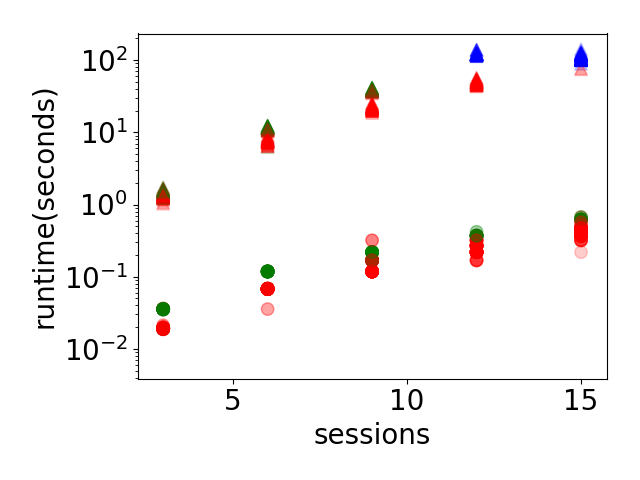
\includegraphics{Sources/transaction/plots/roachdb_sessions.png}
  }
  \caption{Sessions.}
  \label{ser_node_scale}
 \end{subfigure}
 \hspace{-3mm}
 \begin{subfigure}{.33\textwidth}
  \resizebox{\textwidth}{!}{
   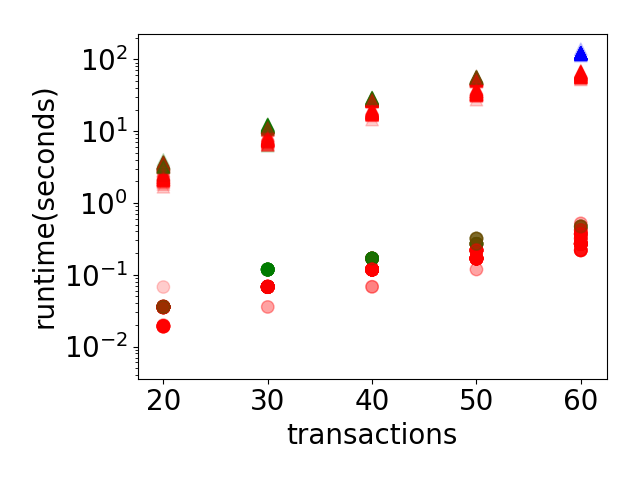
\includegraphics{Sources/transaction/plots/roachdb_transactions.png}
  }
  \caption{Transactions per session.}
  \label{ser_transaction_scale}
 \end{subfigure}

 \begin{subfigure}{.33\textwidth}
  \resizebox{\textwidth}{!}{
   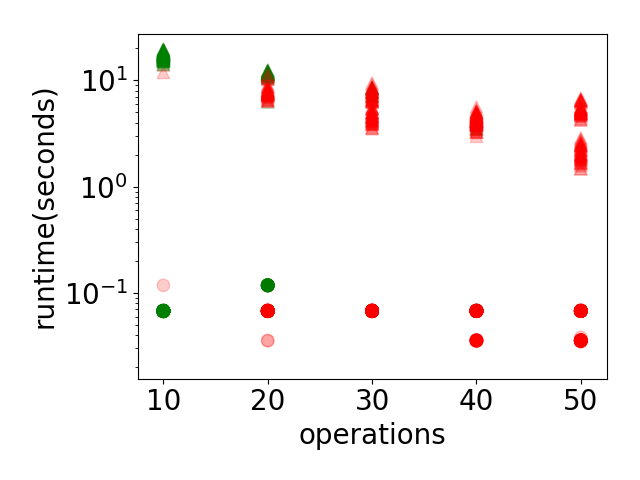
\includegraphics{Sources/transaction/plots/roachdb_operations.png}
  }
  \caption{Operations per transaction.}
  \label{ser_operation_scale}
 \end{subfigure}
 \hspace{-3mm}
 \begin{subfigure}{.33\textwidth}
  \resizebox{\textwidth}{!}{
   \includegraphics{Sources/transaction/plots/roachdb_variables.png}
  }
  \caption{Variables.}
  \label{ser_variable_scale}
 \end{subfigure}
% \begin{subfigure}{.33\textwidth}
%  \resizebox{\textwidth}{!}{
%   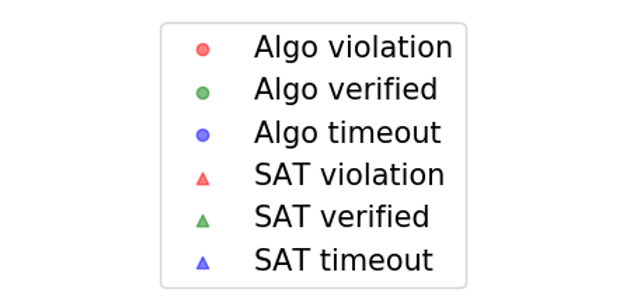
\includegraphics[scale=0.5]{plots/legends.png}
%  }
%  \caption{Legends}
%  \label{legend_1}
% \end{subfigure}
 \vspace{-3mm}
 \caption{Scalability of our algorithm for checking \textsc{Serializability} (Algorithm~\ref{seralgo:2}) with comparison to a SAT encoding. The x-axis represents the varying parameter while the y-axis represents the wall-clock time in logarithmic scale. The circular, resp., triangular, dots represent wall-clock times of our algorithm, resp., the SAT encoding. The red, green, and blue dots represent invalid, valid and resource-exhausted instances, respectively.}
 \label{ser_performace_scale}
 \vspace{-3mm}
\end{figure}


To demonstrate the practical value of the theory developed in the previous sections, we argue that our algorithms:
\begin{itemize}
 \item are efficient and scalable, %and they outperform a SAT encoding of the axioms in Section~\ref{sec:def},
 \item enable an effective testing framework allowing to expose consistency violations in production databases.
\end{itemize}

We focus on three of the criteria introduced in Section~\ref{sec:def}: \emph{serializability} which is NP-complete in general and polynomial time when the number of sessions is considered to be a constant, \emph{snapshot isolation} which can be reduced in linear time to serializability, and \emph{causal consistency} which is polynomial time in general.
%\footnote{Our implementation is publicly available. URL omitted to maintain anonymity.}. 
As benchmark, we consider histories extracted from three distributed databases: CockroachDB~\cite{cockroach}, Galera~\cite{galera}, and AntidoteDB~\cite{antidote}. %\footnote{The databases are deployed using Docker.}.
% snapshot isolation, and causal consistency, and histories extracted from three distributed databases, CockroachDB~\cite{cockroach}, Galera~\cite{galera}, and AntidoteDB~\cite{antidote}.
% which implement serializability~\cite{cockroach-claim}, snapshot isolation~\cite{galera-claim} and causal consistency~\cite{antidote-claim}, respectively (with the default configuration). Therefore, all experiments concerning SER, SI, or CC use histories of CockroachDB, Galera, and AntidoteDB, respectively.
%
% how the histories are generated and executed
%sessions are uniformly distributed among all nodes of the considered distributed database
Following the approach in Jepsen~\cite{jepsen},  histories are generated with random clients. For the experiments described hereafter, the randomization process is parametrized by: (1) the number of sessions ({\bf \#sess}), (2) the number of transactions per session ({\bf \#trs}), (3) the number of operations per transaction ({\bf \#ops}), and (4) an upper bound on the number of used variables ({\bf \#vars})\footnote{We ensure that every value is written at most once.}. For any valuation of these parameters, half of the histories generated with CockroachDB and Galera are restricted such that the sets of variables written by any two sessions are disjoint (the sets of read variables are not constrained). This restriction is used to increase the frequency of valid histories. 
%We also insert a random pause of at most 200 milliseconds between every two transactions within the same session.
%\begin{itemize}
% \item A session is generated by choosing uniformly at random the type of the operations in each transaction (read or write), the variable accessed by each operation, and a value for each write operation. We ensure that every value is written at most once by a client by maintaining a counter map for each variable. 
% \item Each session writes on specific non-overlapping sets of variables of equal size. Otherwise, everything is same as before. A read and write operation are chosen randomly.
%\end{itemize}
%We consider the second type of histories is to increase the number of valid histories in CockroachDB and Galera, because they often produce inconsistent histories. Each history are generated separately as first and then it is executed on the mentioned databases. We used Docker to deploy these distributed instances. 
%Also, we insert a random pause of at most 200 milliseconds between every two transactions within the same session so that the network does not clog up. 

%Then, each executed history is verified with 10 minutes of time limit, 10GB of memory limit and 10GB of file size limit(to avoid big CNF files).

% ser
In a first experiment, we investigated the efficiency of our serializability-checking algorithm (Algorithm~\ref{seralgo:2}) and we compared its performance with a direct SAT encoding\footnote{For each ordered pair of transactions $\tr_1$, $\tr_2$ we add two propositional variables representing $\tup{\tr_1,\tr_2} \in (\wro \cup \so)^+$ and $\tup{\tr_1,\tr_2} \in \CO$, respectively. Then we generate clauses corresponding to: (1) singleton clauses defining the relation $\wro \cup \so$ (extracted from the input history), (2) $\tup{\tr_1, \tr_2} \in \wro \cup \so$ implies $\tup{\tr_1, \tr_2} \in \CO$, (3) $\CO$ being a total order, and (4) the axioms corresponding to the considered consistency model. This is an optimization that does not encode $\wro$ and $\so$ separately, which is sound because of the shape of our axioms (and because these relations are fixed apriori).} of the serializability definition in Section~\ref{sec:def} (we used MiniSAT~\cite{DBLP:conf/sat/EenS03} to solve the SAT queries). We used histories extracted from CockroachDB which claims to implement serializability, acknowledging however the possibility of anomalies~\cite{cockroach-claim}. The sessions of a history are uniformly distributed among 3 nodes of a single cluster. To evaluate scalability, we fix a reference set of parameter values: {\bf \#sess}=6, {\bf \#trs}=30, {\bf \#ops}=20, and {\bf \#vars} = 60 $\times$ {\bf \#sess}, and vary only one parameter at a time. For instance, the number of sessions varies from 3 to 15 in increments of 3. 
We consider 100 histories for each combination of parameter values. The experimental data is reported in Figure~\ref{ser_performace_scale}. Our algorithm scales well even when increasing the number of sessions, which is not guaranteed by its worst-case complexity (in general, this is exponential in the number of sessions). Also, our algorithm is at least two orders of magnitude more efficient than the SAT encoding. While the performance of SAT solvers is known to be heavily affected by the specific encoding of the problem, we strove to make the SAT formula as succinct as possible and optimize its construction.
We have fixed a 10 minutes timeout, a limit of 10GB of memory, and a limit of 10GB on the files containing the formulas to be passed to the SAT solver. The blue dots represent resource-exhausted instances. The SAT encoding reaches the file limit for 148 out of 200 histories with at least 12 sessions (Figure~\ref{ser_node_scale}) and for 50 out of 100 histories with 60 transactions per session (Figure~\ref{ser_transaction_scale}), the other parameters being fixed as explained above. 
 % .(i.e.,  {\bf \#sess}=6, {\bf \#ops}=20, and {\bf \#vars} = 360).

We have found a large number of violations, whose frequency increases with the number of sessions, transactions per session, or operations per transaction, and decreases when allowing more variables. This is expected since increasing any of the former parameters increases the chance of interference between different transactions while increasing the latter has the opposite effect. The second and third column of Table~\ref{violation_stat} give a more precise account of the kind of violations we found by identifying for each criterion X, the number of histories that violate X but no other criterion weaker than X, e.g., there is only one violation to SI that satisfies PC.

%They show our algorithm outperforming SAT encoding by almost 100 times.   In the plots for session, transactions, and events, we see more red plots to the right, this is because increasing these parameters adds more concurrent collisions in the system. If the number of variables is increased, the collisions decrease. Therefore, in the plot of the number of variables, we see green plots in the right. 198 histories with very big SAT instances exhausted memory limit and the average total number of non-empty committed transactions in those histories is 360.

%The main drawback of the SAT encoding is to generate all boolean variables for all possible relation. Usually, just the generation part of the SAT verifier spends more time than our verifier algorithm. Since our algorithms for SER are polynomial time for a fixed number of sessions, their scalability when the number of sessions increases may be an issue, at least in theory. 
%To test our algorithm, we fixed a reference parameter of 6 sessions, 30 transactions per session, 20 operations per transactions, and 60 variables per session. For each parameter, we vary the number of sessions only, keeping the other parameters fixed with this reference parameter and execute 100 different histories (50 of the first type of history and 50 of the second type) for each of them. To complete, we did similar experiments for other parameters as well. Our experimental data are plotted in Figure~\ref{ser_node_scale},~\ref{ser_transaction_scale},~\ref{ser_operation_scale}, and~\ref{ser_variable_scale}. The circular dots are our algorithm runtime, the triangle dots are SAT runtime. We plotted the varying parameter on the x-axis and plotted the verification duration on the y-axis in logarithmic scale. They show our algorithm outperforming SAT encoding by almost 100 times.  The red, green and blue plots are invalid, valid and resource exhausted instances. In the plots for session, transactions, and events, we see more red plots to the right, this is because increasing these parameters adds more concurrent collisions in the system. If the number of variables is increased, the collisions decrease. Therefore, in the plot of the number of variables, we see green plots in the right. 198 histories with very big SAT instances exhausted memory limit and the average total number of non-empty committed transactions in those histories is 360.


\begin{figure}
 \begin{subfigure}{.33\textwidth}
  \resizebox{\textwidth}{!}{
  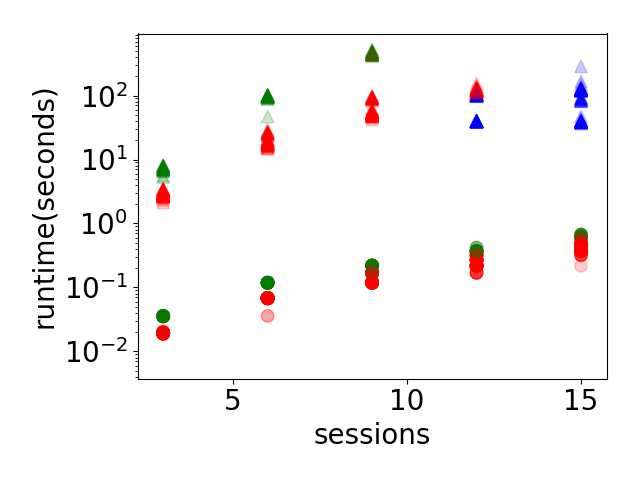
\includegraphics{Sources/transaction/plots/roachdb_si_sessions.png}
  }
  \caption{Checking SI (CockroachDB)}
  \label{roach_si_node_scale}
 \end{subfigure}
 \hspace{-2mm}
 \begin{subfigure}{.33\textwidth}
  \resizebox{\textwidth}{!}{
   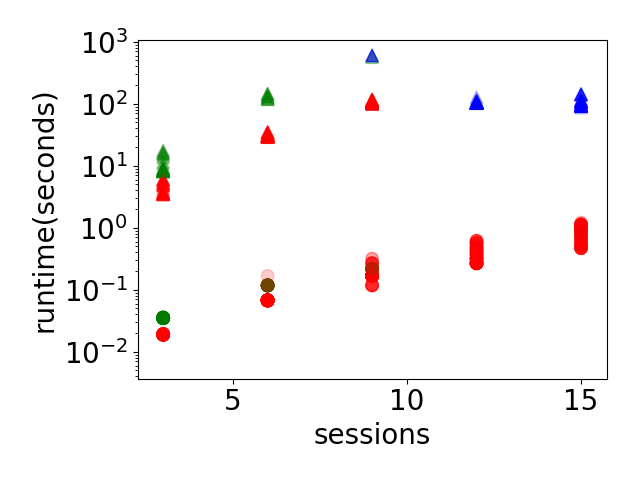
\includegraphics{Sources/transaction/plots/galera_sessions.png}
  }
  \caption{Checking SI (Galera)}
  \label{galera_si_node_scale}
 \end{subfigure}
  \hspace{-2mm}
 \begin{subfigure}{.33\textwidth}
  \resizebox{\textwidth}{!}{
   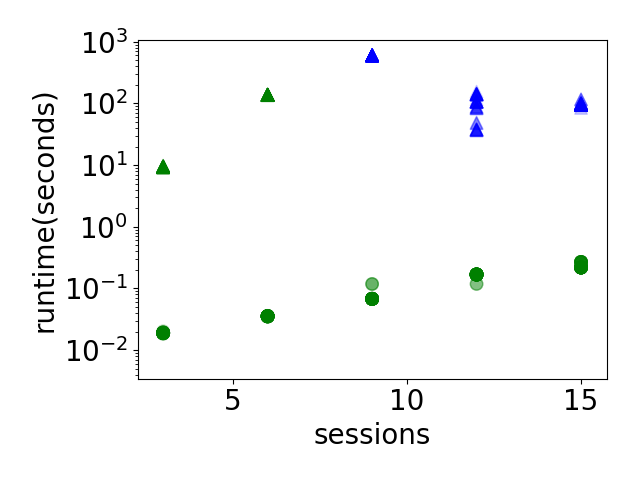
\includegraphics{Sources/transaction/plots/antidote_sessions.png}
  }
  \caption{Checking CC (AntidoteDB)}
  \label{cc_session_scale}
 \end{subfigure}
% \vspace{-3mm}
% \begin{subfigure}{.33\textwidth}
%  \resizebox{\textwidth}{!}{
%   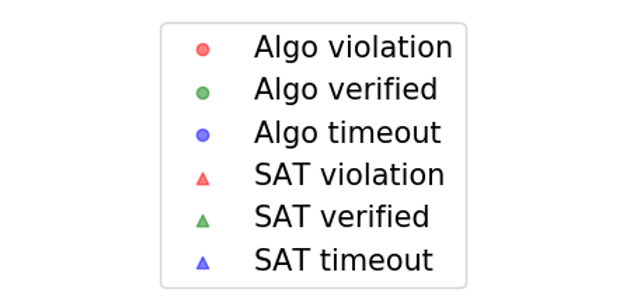
\includegraphics[scale=0.5]{plots/legends.png}
%  }
%  \caption{Legends}
%  \label{legend_2}
% \end{subfigure}
% \vspace{-2mm}
 \caption{Scalability of our algorithms for checking \textsc{Snapshot isolation} (Section~\ref{ssec:si}) and  \textsc{Causal consistency} (Algorithm~\ref{ccalgo:1}) with comparison to a SAT encoding. The x-axis represents the varying parameter while the y-axis represents the wall-clock time in logarithmic scale. The circular, resp., triangular, dots represent wall-clock times of our algorithm, resp., the SAT encoding. The red, green, and blue dots represent invalid, valid and resource-exhausted instances, respectively.}
 \label{si_cc_performace_scale}
\end{figure}

The second experiment measures the scalability of the SI checking algorithm obtained by applying the reduction to SER described in Section~\ref{ssec:si} followed by the SER checking algorithm in Algorithm~\ref{seralgo:2}, and its performance compared to a SAT encoding of SI. Actually, the reduction to SER is performed on-the-fly, while traversing the history and checking for serializability (of the transformed history). The SAT encoding follows the same principles as in the case of serializability. We focus on its behavior when increasing the number of sessions (varying the other parameters leads to similar results). As benchmark, we used the same CockroachDB histories as in Figure~\ref{ser_node_scale} and a number of histories extracted from Galera\footnote{In order to increase the frequency of valid histories, all sessions are executed on a single node.} whose documentation contains contradicting claims about whether it implements snapshot isolation~\cite{galera-claim,galera-notclaim}. We use 100 histories per combination of parameter values as in the previous experiment. The results are reported in Figure~\ref{roach_si_node_scale} and Figure~\ref{galera_si_node_scale}. We observe the same behavior as in the case of SER. In particular, the SAT encoding reaches the file limit for 150 out of 200 histories with at least 12 sessions in the case of the CockroachDB histories, and for 162 out of 300 histories with at least 9 sessions in the case of the Galera histories. The last two columns in Table~\ref{violation_stat} classify the set of violations depending on the weakest criterion that they violate.

We also evaluated the performance of the CC checking algorithm in Section~\ref{sec:general} when increasing the number of sessions, on histories extracted from AntidoteDB, which claims to implement causal consistency~\cite{antidote-claim}. The results are reported in Figure~\ref{cc_session_scale}. In this case, the SAT encoding reaches the file limit for 150 out of 300 histories with at least 9 sessions. All the histories considered in this experiment are valid. However, when experimenting with other parameter values, we have found several violations. The smallest parameter values for which we found violations were 3 sessions, 14 transactions per session, 14 operations per transaction, and 5 variables. The violations we found are also violations of Read Atomic. For instance, one of the violations contains two transactions $\tr_1$ and $\tr_2$, each of them writing to two variables $x_1$ and $x_2$, and another transaction $\tr_3$ that reads $x_1$ from $\tr_1$ and $x_2$ from $\tr_2$ ($\tr_1$ and $\tr_2$ are from different sessions while $\tr_3$ is an $\so$ successor of $\tr_1$ in the same session). These violations are novel and they were confirmed by the developers of AntidoteDB.

%are of this form - two committed transactions, $\tr_1$ and $\tr_2$, write on two variables $x_1$ and $x_2$, then one another transaction, $\tr_3$, reads $x_1$ from $\tr_1$ and $x_2$ from $\tr_2$. These violations are of ReadAtomic consistency. These violations are novel and they were confirmed by the developers of AntidoteDB.
%Similar to SER, we experimented for SI algorithm on Galera and CC algorithm on AntidoteDB as well. 
%%We chose 1 node for Galera (to get more valid histories) and 3 nodes for AntidoteDB. Since SI algorithm is similar to SER and CC algorithm is polytime, we only experimented on the scaling the number of sessions keeping the other parameters fixed. Figure~\ref{si_cc_performace_scale} shows they are performed as expected under session scaling and outperformed SAT encoding. Similar to SER, we also saw some memory limit exhausting SAT instances. 
%162 out of 250 and 150 out of 250 histoies exhausted resource limit for the SI verification of Galera and the CC verification of AntidoteDB respectively. The average total number of transactions in such histories are 402 and 361 for Galera and AntidoteDB respectively.

%Our testing infrastructure was able to find violations of all these criteria meaning that none of the databases we considered satisfies the guarantees stated in the documentation. In Table~\ref{violation_stat}, the violations are very frequent and much weaker than the guarantees for CockroachDB and Galera (more than half of the generated histories) and very rare for AntidoteDB. Actually, for AntidoteDB, the smallest parameter values for which we found violations were 3 sessions, 14 transactions per session, 14 operations per transaction, and at most 5 variables and these violations are of ReadAtomic consistency. These violations were exposed with a frequency of around 20 out of 1000 histories. In the case of CockroachDB, the documentation admits possible anomalies while in the case of Galera, consistency violations were already reported in an open issue on Github~\cite{galera-issue}. The CC violations we found in AntidoteDB are novel and have been confirmed by its developers.

%\begin{figure}
% \resizebox{.45\textwidth}{!}{
%  \includegraphics{plots/roachdb_variables}
% }
% \vspace{-3mm}
% \caption{TODO: add figure Bicomponent decomposition comparison}
% \label{bic_plot}
% \vspace{-2mm}
%\end{figure}

%TODO We don't consider the communication graph story since this requires a deployment on a large cluster which our proof of concept prototype cannot handle.

The refinement of the algorithms above based on communication graphs, described in Section~\ref{sec:communication}, did not have a significant impact on their performance. The histories we generated contained few biconnected components (many histories contained just a single biconnected component) which we believe is due to our proof of concept deployment of these databases on a single machine that did not allow to experiment with very large number of sessions and variables. 

%Lastly, we used our bicomponent technique to scale our algorithm for large histories with relatively less shared variables across the sessions. We present the plot for the runtime of the algorithm with and without bicomponent decomposition in Figure~\ref{bic_plot}.

\begin{table}
\caption{Violation statistics. The ``disjoint writes'' columns refer to histories where the set of variables written by any two sessions are disjoint.}
\small{
 \begin{tabular}{|l|c|c|c|c|c|}
  \hline
  & \multicolumn{2}{c|}{Serializability checking} & \multicolumn{2}{c|}{Snapshot Isolation checking} \\
  \hline
  Weakest                  & CockroachDB     & CockroachDB     & Galera      & Galera                \\
  criterion violated         & (disjoint writes) & (no constraints) & (disjoint writes) & (no constraints)  \\
  \hline
  Read Committed     &             &             & 19          & 50              \\
  Read Atomic        & 180         & 547         & 91          & 139                \\
  Causal Consistency            & 339         & 382         & 88          & 43                  \\
  Prefix Consistency            & 2           & 7           &             &                    \\
  Snapshot Isolation &             & 1           &             & 1                   \\
  Serializability      & 25          &             &            &                     \\
  \hline
%  Serializable      & 454         & 63          & 48          & 16                \\
  \hline
  Total number of violations           & 546/1000        & 937/1000        & 198/250         & 233/250              \\
  \hline
 \end{tabular}
 }
% \vspace{1mm}
 \label{violation_stat}
\end{table}

%We also computed the overheads of running our algorithms on real executions. On the CockroachDB (serializability) it is 0.83\% in average \ie out algorithm takes in average 0.83\% of the execution duration of one single history. For Galera, this value 4.6\%. For AntidoteDB, it is 2.5\%.  


%We verified three databases - AntidoteDB for Causal consistency, Galera for Snapshot isolation, CockroachDB for Serializability. We used Docker to deploy distributed instances. Using our implementation we found,
%
%\begin{itemize}
% \item Rarely AntidoteDB fails to maintain Casusal consistency for big parameters for transactions per node and operations per transaction. In our testing, the lowest paramter that violate this is (X, X, X, X). We tested XXX many case of that paramter and found YYY many violation. We also observed, the violation actually is of Read Atomic. 
% \item We tested 17809 many histories for Galera. 8991 many of them read writes from aborted transactions, read from other transactions after a write internally or do not maintain repeatable read. As of the Snapshot isolation we found 2301 many violations among 8818 many case which do not violate the above case.
% \item We tested many histories of CockroachDB. It never violate the cases mentioned for Galera. But out of 17000 many executions we found 12084 violations of Serializability.
%\end{itemize}
%
%
%
%
%
%We choose $(3,5,5,5)$ as our base parameters for number of nodes, number of transactions per node, number of operations per transaction, number of variables resp. We scale only one parameters and fix other parameter. For each database, we generated 1000 histories for each paramter and executed the generated histories and record the observed histories.
%
%Then we used our implementation to verify the said executions and recorded the durations for each history our algorithm took to finish. We plot the mean duration of each paramter in figure \ref{performace_scale}.
%
%
%
%We also compared our implementation with SAT version of the problem. We encode the problem in SAT and solved it with MiniSAT. We randomly picked from 500 from each set of verified and violated executions and solved with MiniSAT. We compare the runtime of SAT with our implementation in figure \ref{vs_sat}. 

  %!TEX root = Thesis.tex

\section{Transactional System}

\cite{DBLP:conf/concur/Cerone0G15} give the first formalization of the criteria we consider in this paper, using the specification methodology of \cite{DBLP:conf/popl/BurckhardtGYZ14}. This formalization uses two auxiliary relations, a \emph{visibility} relation which represents the fact that a transaction ``observes'' the effects of another transaction and a \emph{commit order}, also called arbitration order, like in our case. Executions are abstracted using a notion of history that includes only a session order and the adherence to some consistency criterion is defined as the existence of a visibility relation and a commit order satisfying certain axioms. Motivated by practical goals, our histories include a write-read relation, which enables more uniform and in our opinion, more intuitive, axioms to characterize consistency criteria. Our formalizations are however equivalent with those of~\cite{DBLP:conf/concur/Cerone0G15} (a formal proof of this equivalence is presented in the extended version of this paper~\cite{DBLP:journals/corr/abs-1908-04509}). Moreover, \cite{DBLP:conf/concur/Cerone0G15} do not investigate algorithmic issues as in our paper.

\cite{DBLP:journals/jacm/Papadimitriou79b} showed that checking serializability of an execution is NP-complete. Moreover, it identifies a stronger criterion called \emph{conflict serializability} which is polynomial-time checkable. Conflict serializability assumes that histories are given as sequences of operations and requires that the commit order be consistent with a \emph{conflict-order} between transactions defined based on this sequence (roughly, a transaction $\tr_1$ is before a transaction $\tr_2$ in the conflict order if it accesses some variable $\xvar$ before $\tr_2$ does). This result is not applicable to distributed databases where deriving such a sequence between operations submitted to different nodes in a network is impossible.

\cite{DBLP:conf/popl/BouajjaniEGH17} showed that checking several variations of causal consistency on executions of a \emph{non-transactional} distributed database is polynomial time (they also assume that every value is written at most once). 
%The also rely on the specification framework in \cite{DBLP:conf/popl/BurckhardtGYZ14}. 
Assuming singleton transactions, our notion of CC corresponds to the causal convergence criterion in~\cite{DBLP:conf/popl/BouajjaniEGH17}. Therefore, our result concerning CC can be seen as an extension of this result concerning causal convergence to transactions.

There are some works that investigated the problem of checking consistency criteria like sequential consistency and linearizability in the case of shared-memory systems. \cite{DBLP:journals/siamcomp/GibbonsK97} showed that checking linearizability of the single-value register type is NP-complete in general, but polynomial time for executions where every value is written at most once. Using a reduction from serializabilty, they showed that checking sequential consistency is NP-complete even when every value is written at most once. \cite{DBLP:journals/pacmpl/EmmiE18} extended the result concerning linearizability to a series of abstract data types called collections, that includes stacks, queues, key-value maps, etc. Sequential consistency reduces to serializability for histories with singleton transactions (i.e., formed of a single read or write operation). Therefore, our polynomial-time result for checking serializability of bounded-width histories (Corollary~\ref{cor:ser}) implies that checking sequential consistency of histories with a bounded number of threads is polynomial time. The latter result has been established independently by \cite{DBLP:journals/pacmpl/AbdullaAJLNS19}.

The notion of \emph{communication graph} is inspired by the work of \cite{DBLP:journals/pacmpl/ChalupaCPSV18}, which investigates partial-order reduction (POR) techniques for multi-threaded programs. In general, the goal of partial-order reduction~\cite{DBLP:conf/popl/FlanaganG05} is to avoid exploring executions which are equivalent w.r.t. some suitable notion of equivalence, e.g., Mazurkiewicz trace equivalence~\cite{DBLP:conf/ac/Mazurkiewicz86}. They use the acyclicity of communication graphs to define a class of programs for which their POR technique is optimal. The algorithmic issues they explore are different than ours and they don't investigate biconnected components of this graph as in our results.

  %!TEX root = ../../Thesis.tex
\section{Conclusion}
\label{sec:txn:conclusion}

We propose novel logical characterizations of various weak consistency models of transactional system such as \emph{Read Committed} (RC)~\cite{DBLP:conf/sigmod/BerensonBGMOO95}, \emph{Read Atomic} (RA)~\cite{DBLP:conf/concur/Cerone0G15},  \emph{Causal Consistency} (CC)~\cite{DBLP:journals/cacm/Lamport78}, \emph{Prefix Consistency} (PC)~\cite{DBLP:conf/ecoop/BurckhardtLPF15}, \emph{Snapshot Isolation} (SI)~\cite{DBLP:conf/sigmod/BerensonBGMOO95} and Serializability (SER). We also investigate the intractibility of these problems. We prove tractability for some cases, but we also show tractability can be regained by considering histories with a bounded number of sessions. We also demonstrate a runtime performance analysis of an implementation of our algorithms.

  \chapter{Testing Applications That Use Transactional Data Stores}
  \label{chap:dist-app}

  %!TEX root = Thesis.tex
\section{Introduction}
\label{sec:intro}

Data storage is no longer about writing data to a single
disk with a single point of access. Modern applications require not just data
reliability, but also high-throughput concurrent accesses. 
Applications concerning supply chains, banking, etc. use traditional relational databases
for storing and processing data, whereas applications such as social networking
software and e-commerce platforms 
use cloud-based storage systems (such as Azure CosmosDb \cite{cosmosdb}, Amazon DynamoDb
\cite{decandia2007dynamo}, Facebook TAO \cite{facebook-tao}, etc.). We use the term \textit{storage
system} in this paper to refer to any such database system/service.


%As applications have moved from a single-box environment to the cloud, the notion of
%data persistence has also changed. It is no longer about storing data on a
%single disk with a single point of access. Rather, modern applications such as
%social networking software, e-commerce platforms, cloud micro-services, etc. are built using 
%high-scale storage systems, such as Azure CosmosDb \cite{cosmosdb}, Amazon DynamoDb \cite{amazon-dynamodb}, 
%Facebook TAO \cite{facebook-tao}. Applications such as 
 
%These storage systems, commonly offered by most major cloud providers (such as
%Azure CosmosDb \cite{cosmosdb}, Amazon DynamoDb \cite{amazon-dynamodb}, 
%Facebook TAO \cite{facebook-tao}, etc.)
%create and manage multiple replicas of data. Having multiple replicas offers reliability and prevents
%data loss, but it also offers availability and low-latency accesses by allowing
%different clients to connect with different replicas. 

Providing high-throughput processing, unfortunately, comes at an unavoidable cost of weakening 
the guarantees offered to users.
Concurrently-connected clients may end up observing different views of the same data. 
These ``anomalies'' can be prevented by using a strong \textit{isolation level} 
such as \textit{serializability}, which essentially offers a single view of the
data. However, serializability requires expensive synchronization and incurs a high performance cost. As a
consequence, most storage systems use weaker isolation levels, such as 
{\it Causal Consistency}~\cite{DBLP:journals/cacm/Lamport78,DBLP:conf/sosp/LloydFKA11,antidote-white-paper},
{\it Snapshot Isolation}~\cite{DBLP:conf/sigmod/BerensonBGMOO95}, {\it Read
Committed}~\cite{DBLP:conf/sigmod/BerensonBGMOO95}, etc. for better performance.
In a recent survey of
database administrators \cite{survey}, 86\% of the participants responded that
most or all of the transactions in their databases execute at read committed isolation level.

\begin{figure}
	\begin{minipage}{4.2cm}
		\begin{lstlisting}[basicstyle=\ttfamily\footnotesize,escapeinside={(*}{*)},language=MyLang]
// Append item to cart
AddItem(item i, userId) {
  Begin()
  key = "cart:" + userId
  cart = read(key)
  cart.append(i)
  write(key, cart)
  Commit()
}
		\end{lstlisting}
	\end{minipage}
	\hspace{-5mm}
	\begin{minipage}{4.2cm}
		\begin{lstlisting}[xleftmargin=4mm,basicstyle=\ttfamily\footnotesize,escapeinside={(*}{*)},language=MyLang]
// Fetch cart and delete item
DeleteItem(item i, userId) {
  Begin()
  key = "cart:" + userId
  cart = read(key)
  cart.remove(i)
  write(key, cart)
  Commit()
}
		\end{lstlisting}
	\end{minipage}
	
\vspace{-6mm}	
  \resizebox{8.5cm}{!}{
   \begin{tikzpicture}[->,>=stealth',shorten >=1pt,auto,node distance=4cm,
     semithick, transform shape]
    \node (s11l) at (1.15, 2.1) {\textbf{Initial state}};
    \node[draw, rounded corners=2mm] (t0) at (2.05, 1.5) {\begin{tabular}{l} $\wrt{\texttt{cart:}u}{\{..\, I\, ..\}}$ \end{tabular}};
    \node[draw, rounded corners=2mm, minimum width=3.6cm, minimum height=1.3cm] (s1) at (0, -0.1) {};
    \node[style={inner sep=0,outer sep=0}] (s11) at (0, 0.3) {\begin{tabular}{l} $\rd{\texttt{cart:}u}{\{..\, I\, ..\}}$\end{tabular}};
    \node[style={inner sep=0,outer sep=0}] (s12) at (0, -0.5) {\begin{tabular}{l} $\wrt{\texttt{cart:}u}{\{..\, I,I\, ..\}}$ \end{tabular}};
    \node (s11l) at (-1, 0.8) {\textbf{AddItem}};
    \node[draw, rounded corners=2mm, minimum width=3.6cm, minimum height=1.3cm] (s2) at (4.1, -0.1) {};
    \node[style={inner sep=0,outer sep=0}] (s21) at (4.1, 0.3) {\begin{tabular}{l} $\rd{\texttt{cart:}u}{\{..\, I\, ..\}}$ \end{tabular}};
    \node[style={inner sep=0,outer sep=0}] (s22) at (4.1, -0.5) {\begin{tabular}{l} $\wrt{\texttt{cart:}u}{\{..\, ..\}}$ \end{tabular}};
    \node (s11l) at (4.9, 0.8) {\textbf{DeleteItem}};
    \node[draw, rounded corners=2mm] (r1) at (8.3, 0) {\begin{tabular}{l} $\rd{\texttt{cart:}u}{\{..\, ..\}}$ \end{tabular}};
    \node[draw, rounded corners=2mm] (r2) at (8.3, -1.3) {\begin{tabular}{l} $\rd{\texttt{cart:}u}{\{..\, I, I\, .\}}$ \end{tabular}};
    \path (s11) edge[left] node {$\po$} (s12);
    \path (s21) edge[left] node {$\po$} (s22);
    \path (t0) edge[left] node {$\wro$} (s1);
    \path (t0) edge[right] node {$\wro$} (s2);
    \path (r1) edge[left] node {$\so$} (r2);
    \path (s2) edge[above] node {$\wro$} (r1);
    \path (s1) edge[below,bend right=11] node {$\wro$} (r2);
%    \path (t0) edge[red, right, bend left=20] node[pos=0.4,xshift=-1] {$\wro$} (s11);
%    \path (t0) edge[red, left, bend right=20] node[pos=0.9,xshift=-1] {$\wro$} (s12);
   \end{tikzpicture}  
  }

%  \begin{lstlisting}[xleftmargin=4mm,basicstyle=\ttfamily\footnotesize,escapeinside={(*}{*)},language=MyLang,morekeywords={Test,GetCart}]
%Test: 
%{ AddItem(I, u); GetCart(u); GetCart(u) } || DeleteItem(I, u)
%		\end{lstlisting}
\vspace{-2mm}
	\caption{A simple shopping cart service.}
	\label{fig:motiv}
\vspace{-3mm}
\end{figure}

A weaker isolation level allows for more possible behaviors than stronger
isolation levels. It is up to the developers then to ensure that their
application can tolerate this larger set of behaviors. Unfortunately, weak
isolation levels are hard to understand or reason about
\cite{DBLP:conf/popl/BrutschyD0V17,adya-thesis} and resulting application bugs
can cause loss of business \cite{acidrain}.
Consider a simple shopping cart application that stores a per-client shopping
cart in a key-value store (\textit{key} is the client ID and \textit{value} is a
multi-set of items). \figref{motiv} shows procedures for adding an item to the cart
(\texttt{AddItem}) and deleting \textit{all} instances of an item from the cart
(\texttt{DeleteItem}). Each procedure executes in a transaction, represented by
the calls to \texttt{Begin} and \texttt{Commit}. Suppose that initially, a user $u$ has 
a single instance of item $I$ in their cart.
Then the user connects to the application via two different
sessions (for instance, via two browser windows), adds $I$ in one session
(\texttt{AddItem($I$, $u$)}) and deletes $I$ in the other session
(\texttt{DeleteItem($I$, $u$)}). With serializability, the cart can either be
left in the state $\{ I \}$ (delete happened first, followed by the add) or $\emptyset$ (delete
happened second). However, with causal consistency (or read committed), it is possible that with two
sequential reads of the shopping cart, the cart is empty in the first read
(signaling that the delete has succeeded), but there are \textit{two} instances of $I$ 
in the second read! Such anomalies, of deleted items reappearing, have been
noted in previous work \cite{decandia2007dynamo}. 

\paragraph{Testing storage-based applications}
This paper addresses the problem of \textit{testing} code for correctness
against weak behaviors: a developer should be able to write a test that runs
their application and then asserts for correct behavior. 
The main difficulty today is getting coverage of weak behaviors during
the test. If one runs the test
against the actual production storage system, it is very likely to only result in
serializable behaviors because of their optimized implementation. For
instance, only 0.0004\% of all reads performed on Facebook's TAO storage system 
were not serializable \cite{facebook-consistency}. 
Emulators, offered by cloud providers for local development, on the other hand, do not support weaker
isolation levels at all \cite{cosmosdb-local}. Another option, possible when
the storage system is available open-source, is to set it up with a 
tool like Jepsen~\cite{jepsen} to inject noise (bring down replicas or
delay packets on the network). 
This approach is unable to provide good coverage at the level of client operations
\cite{clotho} (\sectref{oltp}). Another line of work has focussed on finding
anomalies by identifying non-serializable behavior (\sectref{related}). Anomalies, however, do not
always correspond to bugs \cite{DBLP:conf/pldi/BrutschyD0V18,isodiff}; they may
either not be important (e.g., gather statistics) or may already be handled in
the application (e.g., checking and deleting duplicate items).

%Prior work on this problem has largely focussed on
%formal verification techniques: to establish correctness of code against a specification 
%of a particular isolation level \cite{clotho,maryam} (\akash{others?}). Verification requires
%statically analyzing application code; with such an approach, in addition to
%scalability problems, it is often difficult to support
%various programming styles, libraries, frameworks and languages. 
%For these reasons, testing is still the more widely adopted engineering practice. 
%Our goal is support testing of any application, with little to no modifications.
%We defer more details to the related work section.


%
%There 
%is informal documentation available \cite{cosmosdb-consistency} as well as
%formal specifications \akash{cite CosmosDb-TLA}, but none of it is immediately 
%actionable for a developer. 


%Modern applications such as social networking, ecommerce, etc., use
%highly-available low-latency geo-replicated storage systems~\cite{cosmosdb} to
%achieve high performance and scalability.
%These storage systems must replicate data for persistence, and then allow
%clients to connect with different replicas for availability on failures and for
%low latency.
%The replicas communicate updates to each other in the background using message
%passing.
%However, unfortunately, maintaining strong consistency across these replicas
%requires global synchronization which incurs high performance overheads.
%Moreover, as stated by the Consistency, Availability, and Partition-tolerance
%(CAP) theorem~\cite{cap-theorem},
%it is not possible for such storage systems to remain available and
%simultaneously guarantee consistency under network partitions (which are
%unavoidable).
%Hence, to provide high availability and low latency, many distributed data
%stores provide only weak consistency guarantees, formally defined as different
%consistency models: {\it Causal Consistency}~\cite{constantin-causal,DBLP:journals/cacm/Lamport78},
%{\it Snapshot Isolation}~\cite{DBLP:conf/sigmod/BerensonBGMOO95}, and {\it Read
%Committed}~\cite{DBLP:conf/sigmod/BerensonBGMOO95}, etc.
%This current scenario is also showcased in a recent Database Admin
%Survey~\cite{survey} where more than 73\% participants responded that all the
%transactions in their databases execute at read committed consistency level.

%THE NEXT PARAGRAPH SHOULD BE ONLY ABOUT: PROGRAMMING ON TOP OF WEAK ISOLATION IS HARD. 

%The weak isolation semantics of these consistency models permit various
%anomalies that violate data consistency; for example, lost updates,
%non-repeatable reads etc. 
%(DIRTY READS IS NOT AN ANOMALY ABOVE READ COMMITTED).
%Such anomalies often lead to undesirable executions in client applications and manifest in the form of invariant violations (assertion violations).
%For example, consider an online store with a shopping cart
%service~\ref{fig:motiv}.
%If a user is accessing the cart from multiple clients, and deletes an item from
%one client. 
%Under weak consistency, not only that delete operation can take some time to be
%visible through another client, but even after viewing deletion, the item could
%appear again in the cart \cite{decandia2007dynamo}.
%%\textcolor{blue}{Shopping cart example showing assertion violation on weak consistency.}
%To prevent them, developers should be aware of such anomalies and use explicit
%synchronization at appropriate program points in their applications. 
%(TODO: LOCKING IS TOO SPECIFIC, USE SYNCHRONIZATION INSTEAD).
%This requirement makes application development extremely challenging, because
%such weak isolation semantics are hard to understand and
%reason~\cite{DBLP:conf/popl/BrutschyD0V17,adya-thesis}, compared to the simple case of
%serializability where one can argue about one transaction at a time. Further,
%often these consistency levels are informally explained with low-level
%implementation details, leading to poor understanding.
%For example, Cosmos DB~\cite{cosmosdb} defines five levels of consistency with
%only rough guidelines on which one to pick~\cite{cosmosdb-consistency}.
%(THE FLOW IS A LITTLE BIT AKWARD: WEAK ISOLATION IS HARD TO UNDERSTAND COMPARED TO SERIALIZABILITY; MENTION THE Cosmos DB STUFF AS SUPPORT => INSERTING THE RIGHT SYNCHRONIZATION IS HARD => APPLICATION DEVELOPMENT IS HARD. WHY IS TESTING HARD BECAUSE WEAK ISOLATION IS COMPLICATED ?) 

We present MonkeyDB, a mock in-memory storage system meant for testing
correctness of storage-backed applications. 
MonkeyDB supports 
common APIs for accessing data (key-value updates, as well as SQL queries),
making it an easy substitute for an actual storage system. MonkeyDB
can be configured with one of several isolation levels. 
%Currently,
%MonkeyDB supports Serializability, Causal Consistency as well as Read
%Committed. (Addition of other isolation levels is easy.)
On a read operation, MonkeyDB computes the set of all possible return values
allowed under the chosen isolation level, and randomly returns one of them. The
developer can then simply execute their test multiple times to get coverage of
possible weak behaviors. For the program in \figref{motiv}, if we write a test
asserting that two sequential reads cannot return empty-cart followed by $\{I,
I\}$, then it takes only 20 runs of the test (on average) to fail the
assert. In contrast, the test does not fail when using MySQL with read committed, 
even after 100k runs. 
%MonkeyDB can work with any application with little to no modifications:
%a developer simply needs to link their tests to MonkeyDB, instead of the
%production storage system.

\paragraph{Design of MonkeyDB}
MonkeyDB does not rely on stress generation, fault
injection, or data replication. 
Rather, it works directly with a formalization of
the given isolation level in order to compute allowed return values. 


%MonkeyDB makes it straightforward
%to unit test any storage-backed application. Testing, as opposed to formal
%verification, is still the more widely adopted engineering practice. 

%Given these concerns, we propose our idea {\emph \tool{}}, 
% an in-memory storage system meant for testing. 
%It offers the same interface as most databases (both SQL and Key-Value stores). 
%Internally, it uses a generative model of various (configurable) consistency levels. 
%On read operations, it can systematically pick from the set of all values valid under the given consistency level. 
%%a database model which systematically explores possible behaviors allowed by the used consistency model 
%% and allows developers to check whether their application invariants hold with respect to these possible executions, providing high coverage.
%\tool{} can be used for exhaustive testing (by enumerating all possible read values) or randomized testing that provides much better coverage than otherwise (THIS STATEMENT IS STRONG AND NEEDS SUPPORT).
%%{\tool{}} works as an operational model 
%%and provides the interface of an actual database to any client application. 
%Our design choice addresses above-mentioned concerns and is advantageous in several ways.
%First, it does not need to access the internals of any real database.
%Further, it requires no modifications to the client application under test.
%Furthermore, we can use the same model for a number of databases which leads to effortless testing of client applications against various levels of consistency that are provided by different databases (WHAT DO YOU MEAN BY "SAME MODEL"?) 
%Our design makes \tool{} readily support different modern software architectures such as microservices~\cite{microservice,eshop} where varied databases can be plugged-in and each microservice connects to its own database having a specific consistency model.
%%Our effort is building something that any developer can use by themselves.
%%The key features of \tool{} is:
%% (1) works on real applications directly and requires no modifications to the system under test,
%% (2) expects no expertise from developers because its integration and use is same as that of a real database,
%% (3) provides good coverage,
%% (4) does not report false positives.


%\constantin{FROM THIS POINT ON, WE NEED A "DEEPER" PRESENTATION OF THE THEORY
%  USED IN THE IMPLEMENTATION. STARTING FROM AXIOMATIC SEMANTICS FOR ISOLATION
%  LEVELS IN KEY-VALUE STORES, OPERATIONAL SEMANTICS (STRESS THE SERIAL
%EXECUTION), COMPILING SQL TO KEY-VALUE STORE API. }

The theory behind MonkeyDB builds on the axiomatic definitions of isolation
levels introduced by Biswas et al. \cite{DBLP:journals/pacmpl/BiswasE19}. These
definitions use logical constraints (called \emph{axioms}) to characterize the
set of executions of a key-value store that conform to a particular isolation
level (we discuss SQL queries later). These constraints refer to a specific set of
relations between events/transactions in an execution that describe control-flow
or data-flow dependencies: a program order $\po$ between events in the same
transaction, a session order $\so$ between transactions in the same session\footnote{A
session is a sequential interface to the storage system. It corresponds to what
is also called a connection.}, and a write-read $\wro$ (read-from) relation that
associates each read event with a transaction that writes the value returned by
the read. These relations along with the events (also called, operations) in an
execution are called a \emph{history}. The history corresponding to the 
shopping cart anomaly explained above is given on the bottom of Figure~\ref{fig:motiv}.
Read operations include the read value, and boxes group events from the same transaction.
%The initial value of the key is supposed to be written in a fictitious transaction. 
A history describes only the
interaction with the key-value store, omitting application side events (e.g., computing
the value to be written to a key). 

MonkeyDB implements a \emph{centralized} operational semantics for key-value stores, which is based on these axiomatic definitions. Transactions are executed \emph{serially}, one after another, the concurrency being simulated during the handling of read events.  
This semantics maintains a history that contains all the past events (from all
transactions/sessions), and write events are simply added to the history. The
value returned by a read event is established based on a non-deterministic
choice of a write-read dependency (concerning this read event) that satisfies
the axioms of the considered isolation level.
%(MonkeyDB resolves any non-determinism in a random fashion). 
Depending on the weakness of the isolation
level, this makes it possible to return values written in arbitrarily ``old''
transactions, and simulate any concurrent behavior. For instance, the history in Figure~\ref{fig:motiv}
can be obtained by executing \texttt{AddItem}, \texttt{DeleteItem}, and then the two reads (serially).
The read in \texttt{DeleteItem} can take its value from the initial state and ``ignore'' the
previously executed \texttt{AddItem}, because the obtained history validates the axioms of 
causal consistency (or read committed). The same happens for the two later reads in the same
session, the first one being able to read from \texttt{DeleteItem} and the second one
from \texttt{AddItem}.

We formally prove that this semantics does indeed simulate any concurrent behavior, by 
showing that it is equivalent to a semantics where transactions are allowed to interleave.
In comparison with concrete implementations, this semantics makes it possible to handle 
a wide range of isolation levels in a uniform way. It only has two sources of
non-determinism: 
the order in which entire transactions are submitted, and the choice of write-read dependencies in read 
events. This enable better coverage of possible behaviors, the penalty in performance not
being an issue in safety testing workloads which are usually small (see our evaluation). 


We also extend our semantics to cover SQL queries as well, by compiling SQL queries down to transactions with multiple key-value reads/writes. A table in a relational database is represented using a set of primary key values (identifying uniquely the set of rows) and a set of keys, one for each cell in the table. The set of primary key values is represented using a set of Boolean key-value pairs that simulate its characteristic function (adding or removing an element corresponds to updating one of these keys to $\btrue$ or $\bfalse$). Then, SQL queries are compiled to read or write accesses to the keys representing a table. For instance, a $\mathtt{SELECT}$ query that retrieves the set of rows in a table that satisfy a $\mathtt{WHERE}$ condition is compiled to (1) reading Boolean keys to identify the primary key values of the rows contained in the table, (2) reading keys that represent columns used in the $\mathtt{WHERE}$ condition, and (3) reading all the keys that represent cells in a row satisfying the $\mathtt{WHERE}$ condition. This rewriting contains the minimal set of accesses to the cells of a table that are needed to ensure the conventional specification of SQL.
It makes it possible to ``export'' formalizations of key-value store isolation levels to SQL transactions.

%This paper first presents an axiomatic semantics for various isolation levels 
%in Key-Value stores that allows one to reason about the set of valid behaviors
%under a given isolation level. We follow this by a non-deterministic operation
%semantics, equivalent to the axiomatic semantics, where
%each operation is cooperatively scheduled to execute one at a time (serially).
%The operational semantics maintains a history of the read-write operations,
%including a \textit{read-from} relationship that matches reads to previous
%writes. On the submission of a new operation, this history is extended in
%accordance with this operational semantics. MonkeyDB implements the operational
%semantics, while resolving any non-determinism in a random fashion. 
%We also extend our semantics to cover SQL queries as well, by compiling SQL
%queries down to transactions with multiple key-value updates.

\paragraph{Contributions}
%We implemented MonkeyDB to support an interface consistent with key-value
%stores and databases, which allows us to directly run real applications unmodified. 
%We evaluated MonkeyDB on a series of micro-benchmarks, inspired from real
%applications, as well as the well-known OLTPBench \cite{difallah2013oltp}
%that is used for evaluating
%databases on OLTP workloads. 

This paper makes the following contributions:
\begin{itemize}
\item We define an operational semantics for key-value stores under various
  isolation levels, which simulates all concurrent behaviors with executions
  where transactions execute serially (\sectref{op-kv}) and which is based 
  on the axiomatic definitions in~\cite{DBLP:journals/pacmpl/BiswasE19} (and outlined in \S\ref{sec:ax-kv}),
\item We broaden the scope of the key-value store semantics to SQL transactions
  using a compiler that rewrites SQL queries to key-value accesses (\sectref{SQL-to-KV}),
\item The operational semantics and the SQL compiler are implemented in a tool
  called MonkeyDB (\sectref{impl}). It randomly resolves possible choices to provide coverage
  of weak behaviors. It supports both a key-value interface as well as SQL,
  making it readily compatible with any storage-backed application.
\item We present an evaluation of MonkeyDB on several applications, showcasing
its superior coverage of weak behaviors as well as bug-finding abilities
(\sectref{micro}, \sectref{oltp}).\footnote{Source code of our benchmarks is available
as supplementary material.}
\end{itemize}



 


 




  %!TEX root = Thesis.tex

\section{Programming Language}\label{sec:app:prog_lang}

\begin{figure}
\small
\begin{align*}
\key\in \Keys\quad \xvar\in\Vars\quad \tab\in\Tables\quad \vec{c},\vec{c_1},\vec{c_2}\in \Columns^*
\end{align*}
\begin{align*}
\mathsf{Prog} &  \eqdef  \mathsf{Sess} \ \mid\  \mathsf{Sess}\,||\,\mathsf{Prog} \\
\mathsf{Sess} & \eqdef  \mathsf{Trans} \ \mid\  \mathsf{Trans}; \mathsf{Sess} \\
\mathsf{Trans} & \eqdef  \ibegin; \mathsf{Body}; \icommit \\
\mathsf{Body} & \eqdef  \mathsf{Instr} \ \mid\  \mathsf{Instr}; \mathsf{Body} \\
\mathsf{Instr} & \eqdef  \mathsf{InstrKV} \ \mid\  \mathsf{InstrSQL}\ \mid\  x := e \mid\ \iif{\phi(\vec{x})}{\mathsf{Instr}} \\
\mathsf{InstrKV} & \eqdef \xvar := \iread(\key)  \ \mid\  \iwrite(\key,\xvar) \\
\mathsf{InstrSQL} & \eqdef  \iselect{\vec{c_1}}{\xvar}{\tab}{\phi(\vec{c_2})} \ \mid\ \\
& \hspace{5mm} \iinsert{\tab}{\vec{x}} \ \mid\ \\
& \hspace{5mm} \idelete{\tab}{\phi(\vec{c})} \ \mid\ \\
& \hspace{5mm} \iupdate{\tab}{\vec{c_1}=\vec{x}}{\phi(\vec{c_2})} 
%\mathsf{Local} & \eqdef  x := e
\end{align*}
\vspace{-6mm}
\caption{Program syntax. The set of all keys is denoted by $\Keys$, $\Vars$ denotes the set of local variables, $\Tables$ the set of table names, and $\Columns$ the set of column names.
We use $\phi$ to denote Boolean expressions, and $e$ to denote expressions interpreted as values. We use $\vec{\cdot}$ to denote vectors of elements.}
\label{fig:syntax}
\vspace{-4mm}
\end{figure}

Figure~\ref{fig:syntax} lists the definition of two simple programming languages that we use to represent applications running on top of Key-Value or SQL stores, respectively. A program is a set of \emph{sessions} running in parallel, each session being composed of a sequence of \emph{transactions}. Each transaction is delimited by $\ibegin$ and $\icommit$ instructions\footnote{For simplicity, we assume that all the transactions in the program commit. Aborted transactions can be ignored when reasoning about safety because their effects should be invisible to other transactions.}, and its body contains instructions that access the store, and manipulate a set of local variables $\Vars$ ranged over using $\xvar$, $\yvar$, $\ldots$.

In case of a program running on top of a Key-Value store, the instructions can be reading the value of a key and storing it to a local variable $\xvar$ ($\xvar := \iread(\key)$) , writing the value of a local variable $\xvar$ to a key ($\iwrite(\key,\xvar)$), or an assignment to a local variable $\xvar$. The set of values of keys or local variables is denoted by $\Vals$. Assignments to local variables use expressions interpreted as values whose syntax is left unspecified. Each of these instructions can be guarded by a Boolean condition $\phi(\vec{x})$ over a set of local variables $\vec{x}$ (their syntax is not important). Other constructs like $\mathtt{while}$ loops can be defined in a similar way. Let $\KVProgs$ denote the set of programs where a transaction body can contain only such instructions.

For programs running on top of SQL stores, the instructions include simplified
versions of standard SQL instructions and assignments to local variables. These
programs run in the context of a \emph{database schema} which is a (partial)
function $\DBschema:\Tables\rightharpoonup 2^\Columns$ mapping table names in
$\Tables$ to sets of column names in $\Columns$. The SQL store is an
\emph{instance} of a database schema $\DBschema$, i.e., a function $\DBinst:
\mathsf{dom}(\DBschema)\rightarrow 2^{\Rows}$ mapping each table $\tab$ in the
domain of $\DBschema$ to a set of \emph{rows} of $\tab$, i.e., functions $r:\DBschema(\tab)\rightarrow\Vals$. We use $\Rows$ to denote the set of all rows.
The $\mathtt{SELECT}$ instruction retrieves the columns $\vec{c_1}$ from the set of rows of $\tab$ that satisfy $\phi(\vec{c_2})$ ($\vec{c_2}$ denotes the set of columns used in this Boolean expression), and stores them into a variable $\xvar$. $\mathtt{INSERT}$ adds a new row to $\tab$ with values $\vec{x}$, and $\mathtt{DELETE}$ deletes all rows from $\tab$ that satisfy a condition $\phi(\vec{c})$. The $\mathtt{UPDATE}$ instruction assigns the columns $\vec{c_1}$ of all rows of $\tab$ that satisfy $\phi(\vec{c_2})$ with values in $\vec{x}$.
Let $\SQLProgs$ denote the set of programs where a transaction body can contain only such instructions.

  % %!TEX root = Thesis.tex
\section{Isolation Levels for Key-Value Stores}
\label{sec:ax-kv}

%We consider a sequence of increasingly stronger isolation levels: Read Atomic, Causal Consistency, Prefix Consistency, Snapshot Isolation, Serializability. In each level, a transaction reads from a snapshot obtained by executing a sequence of transactions atomically (be sure about this intuition). Different levels impose constraints on the relationship between the sequences read by different transactions.
%
%Recall the OOPSLA'19 definitions. Histories as abstractions of executions, and the axioms corresponding to these isolation levels.
%
%Give some theorem about "a transaction reads from a snapshot obtained by executing a sequence of transactions atomically". This is important for explaining why transactions can be executed atomically in the operational semantics.
%
%Give a theorem about "prefix closure": if a history is correct, then it remains correct if we remove a suffix of a session (this suffix does not necessarily contain only entire transactions). This is useful for proving the completeness of the operational semantics.

We present the axiomatic framework introduced in~\cite{DBLP:journals/pacmpl/BiswasE19} for defining isolation levels\footnote{Isolation levels are called consistency models in~\cite{DBLP:journals/pacmpl/BiswasE19}.} in Key-Value stores. Isolation levels are defined as logical constraints, called \emph{axioms}, over \emph{histories}, which are an abstract representation of the interaction between a program and the store in a concrete execution. 
% that record the sequence of reads and writes executed in each transaction, the order between transactions in each session, and a write-read relation (also called read-from) that ``justifies'' read values by associating each read to a write that wrote the value returned by the read.

%TODO SOME INTRO EXPLAINING THAT ISOLATION LEVELS ARE DEFINED AS AXIOMS OVER HISTORIES, WHICH REPRESENT THE INTERACTION BETWEEN A PROGRAM AND A STORE. 

\subsection{Histories}

Programs interact with a Key-Value store by issuing transactions formed of $\textsf{read}$ and $\textsf{write}$ instructions. The effect of executing one such instruction is represented using an \emph{operation}, which is an element of the set
\begin{align*}
 \Op=\set{\rd[\id]{\key}{\val},\wrt[\id]{\key}{\val}: \id\in\OId, \key\in\Keys, \val\in \Val}
\end{align*} 
where $\rd[\id]{\key}{\val}$ (resp., $\wrt[\id]{\key}{\val}$) corresponds to reading a value $\val$ from a key $\key$ (resp., writing $\val$ to $\key$). Each operation is associated with an identifier $\id$ from an arbitrary set $\OId$. We omit operation identifiers when they are not important.

\begin{definition}
 A \emph{transaction log} $\tup{\tr, O, \po}$ is a transaction identifier $\tr$ and a finite set of operations $O$ along with a strict total order $\po$ on $O$, called \emph{program order}.
\end{definition}

The program order $\po$ represents the order between instructions in the body of a transaction. We assume that each transaction log is well-formed in the sense that if a read of a key $k$ is preceded by a write to $\key$ in $\po$, then it should return the value written by the last write to $\key$ before the read (w.r.t. $\po$). This property is implicit in the definition of every isolation level that we are aware of. For simplicity, we may use the term \emph{transaction} instead of transaction log. The  set of all transaction logs is denoted by $\mathsf{Tlogs}$.

%We use $\tr$, $\tr_1$, $\tr_2$, $\ldots$ to range over transaction logs. 

The set of read operations $\rd{\key}{\_}$ in a transaction log $\tr$ that are \emph{not} preceded by a write to $\key$ in $\po$ is denoted by $\readOp{\tr}$. As mentioned above, the other read operations take their values from writes in the same transaction and their behavior is independent of other transactions. Also, the set of write operations $\wrt{\key}{\_}$ in $\tr$ that are \emph{not} followed by other writes to $\key$ in $\po$ is denoted by $\writeOp{\tr}$. If a transaction contains multiple writes to the same key, then only the last one (w.r.t. $\po$) can be visible to other transactions (w.r.t. any isolation level that we are aware of). The extension to sets of transaction logs is defined as usual. 
Also, we say that a transaction log $\tr$ \emph{writes} a key $\key$, denoted by $\writeVar{\tr}{\key}$, when $\wrt[\id]{\key}{\val}\in \writeOp{\tr}$ for some $\id$ and $\val$. 
%Similarly, $\tr$ \emph{reads} $\key$ when $\rd[\id]{\key}{\val}\in \readOp{\tr}$ for some $\id$ and $\val$.



%\begin{figure}[t]
% \centering
% \begin{subfigure}{.21\textwidth}
%   \centering
%  \resizebox{!}{1.3cm}{
%   \begin{tikzpicture}[->,>=stealth',shorten >=1pt,auto,node distance=2cm,
%     semithick, transform shape]
%    \node[draw, rounded corners=2mm] (t1) {\begin{tabular}{l} \texttt{x = 1;} \\ ... \\ \texttt{x = 2;} \end{tabular}};
%    \node[draw, rounded corners=2mm, right of = t1] (t2) {\begin{tabular}{l} ... \\ \texttt{read(x);} \end{tabular}};
%   \end{tikzpicture}  
%  }
%%  \caption{Only the lastest write is visible to other transaction}
%\caption{}
%  \label{rc_eg:1}
% \end{subfigure}
% \hspace{10mm}
% \begin{subfigure}{.1\textwidth}
%   \centering
%  \resizebox{!}{2cm}{
%   \begin{tikzpicture}[->,>=stealth',shorten >=1pt,auto,node distance=2cm,
%     semithick, transform shape]
%    \node[draw, rounded corners=2mm] (t1) {\begin{tabular}{l} \texttt{x = 1;} \\ ... \\ \texttt{x = 2;} \\ ... \\ \texttt{read(x);}\end{tabular}};
%   \end{tikzpicture}  
%  }
%%  \caption{Always reads the latest write inside a transaction}
%\caption{}
%  \label{rr_eg:1}
% \end{subfigure}
% \hspace{10mm}
% \begin{subfigure}{.14\textwidth}
%   \centering
%  \resizebox{!}{1.3cm}{
%   \begin{tikzpicture}[->,>=stealth',shorten >=1pt,auto,node distance=2cm,
%     semithick, transform shape]
%    \node[draw, rounded corners=2mm] (t1) {\begin{tabular}{l} \texttt{x = 1;} \\ ... \\ \texttt{ABORT;} \end{tabular}};
%    \node[draw, rounded corners=2mm, right of = t1] (t2) {\begin{tabular}{l} ... \\ \texttt{read(x);} \end{tabular}};
%   \end{tikzpicture}  
%  }
%%  \caption{Aborted transactions are not visible}
%\caption{}
%  \label{abort:1}
% \end{subfigure}
% \caption{Examples of transactions used to justify our simplifying assumptions (each box represents a different transaction): (a) only the last written value is observable in other transactions, (b) reads following writes to the same variable return the last written value in the same transaction, and (c) values written in aborted transactions are not observable.}
% \label{read_latest}
% \vspace{-3mm}
%\end{figure}

%To simplify the exposition, we assume that each transaction $\tr$ contains at most one write operation to each variable\footnote{That is, for every transaction $\tr$, and every $\wrt{\xvar}{\val}, \wrt{\yvar}{\val'}\in \writeOp{\tr}$, we have that $\xvar\neq\yvar$.}, and that a read of a variable $\xvar$ cannot be preceded by a write to $\xvar$ in the same transaction\footnote{That is, for every transaction $\tr=\tup{O, \po}$, if $\wrt{\xvar}{\val}\in \writeOp{\tr}$ and there exists $\rd{\xvar}{\val}\in \readOp{\tr}$, then we have that $\tup{\rd{\xvar}{\val},\wrt{\xvar}{\val}}\in \po$}. If a transaction would contain multiple writes to the same variable, then only the last one should be visible to other transactions (w.r.t. any consistency criterion considered in practice). For instance, the \texttt{read(x)} in Figure~\ref{rc_eg:1} should not return 1 because this is not the last value written to {\tt x} by the other transaction. It can return the initial value or 2.
%%In figure (\ref{rc_eg:1}), however the two transactions are executed, the operation \texttt{print(x)} in below transaction should not print \texttt{0}. Because \texttt{x=0} is not the latest write in the above transaction.
%Also, if a read would be preceded by a write to the same variable in the same transaction, then it should return a value written in the same transaction (i.e., the value written by the latest write to $\xvar$ in that transaction). 
%For instance, the \texttt{read(x)} in Figure~\ref{rr_eg:1} can only return 2 (assuming that there are no other writes on {\tt x} in the same transaction).
%%In figure (\ref{rr_eg:1}), the operation \texttt{print(x)} in the transaction should not print \texttt{1}, because $\texttt{print(x)}$ is not the latest write to \texttt{print(x)}.
%These two properties can be verified easily (in a syntactic manner) on a given execution. Beyond these two properties, the various consistency criteria used in practice constrain only the last writes to each variable in each transaction and the reads that are not preceded by writes to the same variable in the same transaction.

A \emph{history} contains a set of transaction logs (with distinct identifiers) ordered by a (partial) \emph{session order} $\so$ that represents the order between transactions in the same session\footnote{In the context of our programming language, $\so$ would be a union of total orders. This constraint is not important for defining isolation levels.}. It also includes a
%ordering constraints imposed by the applications using the database. Most often, $\so$ is a union of sequences, each sequence being called a \emph{session}. 
\emph{write-read} relation (also called read-from) that ``justifies'' read values by associating each read to a transaction that wrote the value returned by the read.
%that identifies the transaction writing the value returned by each read in the execution. 

%As mentioned before, such a relation can be extracted easily from executions where each value is written at most once. Since in practice, databases are data-independent~\cite{DBLP:conf/popl/Wolper86}, i.e., their behavior does not depend on the concrete values read or written in the transactions, any potential buggy behavior can be exposed in such executions. 

%Transactions and operations may be failed or aborted. The effects of the failed or aborted transactions and operations should not be visible. So we assume the transactions and operations are always successful or committed. If such transactions and operations exist, we discard them after checking there is no operation that read from failed or aborted transactions or operations. Therefore  In figure (\ref{abort:1}), the left transaction is aborted. So the operation \texttt{print(x)} in the right transaction should not output \texttt{0}. 


%We assume, in each transaction if there is no write before a read, it reads either from the last write of an another transaction or an initial value. Also when a transaction reads a value after a write, it reads from last write before that read. \ie if $\rd{\xvar}{\val} \in \tr_1$ reads from $\wrt{\xvar}{\val} \in \tr_2$, then for any other $\wrt{\xvar}{\_} \in \tr_2$ or $\tr_1$, $\tup{\wrt{\xvar}{\_}, \wrt{\xvar}{\val}} \in O_{\tr_2}$ or $\tup{\rd{\xvar}{\val}, \wrt{\xvar}{\_}} \in O_{\tr_1}$.
%
%Once we have a set of transactions, we can statically check if this is true for all transactions. Then, for all variables, we can ignore all the writes except the final one and all the reads after first write in a transaction. For simplicity, we assume that 



% TODO EXPLAIN THE FOLLOWING SIMPLIFICATIONS: WE DON'T CARE ABOUT MULTIPLE WRITES SINCE ANYWAY, ALL CRITERIA REQUIRE THAT ONLY THE LAST ONE IS VISIBLE. ALSO, ONCE A VARIABLE IS WRITTEN EVERY CRITERION REQUIRES THAT THE READ RETURNS THE INTERNALLY WRITTEN VALUE. ALL THESE THINGS CAN BE CHECKED EASILY IN A SYNTACTIC WAY ON HISTORIES.


%We say that a transaction $\tr$ writes value $\val$ a variable $\xvar$, denoted by $\tr\models \wrt{\xvar}{\val}$, whenever $\wrt{\xvar}{\val}$ is the last write o variable $\xvar$ of $\tr$, i.e., $\wrt{\xvar}{\val}\in \writeOp{\tr}$ and for any $\wrt{\xvar}{\val'}\in \writeOp{\tr}$ with $\val\neq\val'$, we have that $\tup{\wrt{\xvar}{\val'}, \wrt{\xvar}{\val}}\in \po$.
% \item $\tr \models \wrt[\id]{\xvar}{\val} \Leftrightarrow max_{\textsf{po}} \left( \left\{ write(x,\_) \in O \right\} \right) = write(x, n)$
% \item $(O, \textsf{po}) \models \texttt{read}(x, n) \Leftrightarrow min_{\textsf{po}} \left( \left\{ \_(x,\_) \in O \right\} \right) = read(x, n)$
% \item $(O, \textsf{po}) \in Write_{x} \Leftrightarrow \left\{ write(x,\_) \in O \right\} \neq \emptyset$



%When a read operation in a transaction reads a value from an operation from another transaction, it defines a \emph{write-read order} between them. Also, typically a transactional system allows its clients to group their transactions in one single session. This imposes a \emph{session order} on the transactions. We define a client-visible results of an execution of a set of sessions as a \emph{history}.

% TODO SAY THAT HISTORIES CONTAIN ONLY COMMITTED TRANSACTIONS FROM A CONCRETE EXECUTION, THE EFFECTS OF ABORTED TRANSACTIONS ARE NOT VISIBLE.

\begin{definition}
 A \emph{history} $\tup{T, \so, \wro}$ is a set of transaction logs $T$ along with a strict partial \emph{session order} $\so$, and a 
 %surjective\footnote{That is, for all $\rd{\xvar}{\val}\in \readOp{T}$ there exists a transaction $\tr\in T$ such that $\tup{\tr,\rd{\xvar}{\val}}\in \wro$.} 
\emph{write-read} relation $\wro\subseteq T\times \readOp{T}$ such that
the inverse of $\wro$ is a total function, and if $(\tr,\rd{\key}{\val})\in\wro$, then $\wrt{\key}{\val}\in\tr$, and $\so\cup\wro$ is acyclic.
\end{definition}

% TODO SAY THAT INITIAL VALUES ARE ASSUMED TO BE WRITTEN BY A TRANSACTION ORDERED IN SO BEFORE ALL THE OTHER TRANSACTIONS.

%The transactions may try to read a variable, even before there is a write to it. In practice, the databases return a default initialized or null value for those reads. This situation can be thought as if the database wrote that value in an \emph{initialization} transaction, in which all variables are written with an initialized value. So we assume a history contains an initialization transaction. This initialization transaction precedes all other transactions by $\so$.

To simplify the technical exposition, we assume that every history includes a distinguished transaction log writing the initial values of all keys. This transaction log precedes all the other transaction logs in $\so$. We use $\hist$, $\hist_1$, $\hist_2$, $\ldots$ to range over histories. The set of transaction logs $T$ in a history $\hist=\tup{T, \so, \wro}$ is denoted by $\tlogs{\hist}$.

%We say that the read operation $\rd{\key}{\val}$ \emph{reads the value $\val$ of $\key$ written by $\tr$} when $(\tr,\rd{\key}{\val})\in\wro$. 
For a key $\key$, $\wro[\key]$ denotes the restriction of $\wro$ to reads of $\key$, \ie, $\wro[\key]=\wro\cap (T\times \{\rd{\key}{\val}\mid \val\in \Val\})$. Moreover, we extend the relations $\wro$ and $\wro[\key]$ to pairs of transactions by $\tup{\tr_1,\tr_2}\in \wro$, resp., $\tup{\tr_1,\tr_2}\in \wro[\key]$, iff there exists a read operation $\rd{\key}{\val}\in \readOp{\tr_2}$ such that $\tup{\tr_1,\rd{\key}{\val}}\in \wro$, resp., $\tup{\tr_1,\rd{\key}{\val}}\in \wro[\key]$. 
We say that the transaction log $\tr_1$ is \emph{read} by the transaction log $\tr_2$ when $\tup{\tr_1,\tr_2}\in \wro$. % and that it is \emph{read} when it is read by some transaction $\tr_2$. 
%

%A consistency model describes how a transactional system processes transactions. To formally define the behaviors, we will extend history with two relations.

%The definitions of the consistency criteria rely on a few basic notions of sequences and orders. We denote the \emph{prefix} of a sequence $\sigma$ up to and including an element $\alpha$ by $\sigma(\alpha)$, and the \emph{prefix} of a partial order $\pi$ up to and including $\alpha$ by $\pi(\alpha) = \set{\tup{ \alpha_1, \alpha_2 } \in \pi : \tup{\alpha_2, \alpha} \in \pi \text{ or } \alpha_2 = \alpha }$. A sequence $\sigma_1$ is called a \emph{subsequence} of another sequence $\sigma_2$, denoted by $\sigma_1\preceq \sigma_2$, when $\sigma_1$ is obtained from $\sigma_2$ by deleting elements. We extend the notion of subsequence to partial orders and say that an order $\pi_1$ is a \emph{suborder} of another order $\pi_2$ if $\pi_1\subseteq \pi_2$. For uniformity, we write $\pi_1 \preceq \pi_2$ when $\pi_1$ is a suborder of $\pi_2$. The subsequence of a sequence $\sigma$ that includes all the elements ordered between two elements $\alpha_1$ and $\alpha_2$ (including $\alpha_1$ and $\alpha_2$) is denoted by $\sigma[\alpha_1,\alpha_2]$.
%Also, for simplicity, we don’t make the distinction between sequences and total orders, reusing notions like prefix and subsequence in the context of total orders.
%
%\begin{definition}
% A \emph{linearization} $\ell=\tup{\lin,\vis}$ of a history $\tup{T, \so, \wro}$ is a total order $\lin$ on $T$, and a function $\vis$, mapping each transaction $\tr\in T$ to a subsequence of $\lin(\tr)$ including $\tr$.
%\end{definition}
%
%A consistency model is defined as the set of histories which admit linearizations satisfying certain \emph{consistency axioms}. The axioms rely on a few notations
%\begin{itemize}
% \item $\tr \models \wrt[\id]{\xvar}{\val} \Leftrightarrow max_{\textsf{po}} \left( \left\{ write(x,\_) \in O \right\} \right) = write(x, n)$
% \item $(O, \textsf{po}) \models \texttt{read}(x, n) \Leftrightarrow min_{\textsf{po}} \left( \left\{ \_(x,\_) \in O \right\} \right) = read(x, n)$
% \item $(O, \textsf{po}) \in Write_{x} \Leftrightarrow \left\{ write(x,\_) \in O \right\} \neq \emptyset$
%\end{itemize}


\subsection{Axiomatic Framework}

% from Table. \ref{weakconsistency:1}. Table. \ref{weakconsistency:2} lists the axioms of consistency models.

%!TEX root = Thesis.tex
\tikzset{transaction state/.style={draw=black!0}}


 \begin{figure*}
   \resizebox{\textwidth}{!}{
   \footnotesize
  \begin{tabular}{|c|c|c|}
   \hline &  & \\
   \begin{subfigure}[t]{.3\textwidth}
    \centering
    \begin{tikzpicture}[->,>=stealth',shorten >=1pt,auto,node distance=1cm,
      semithick, transform shape]
     \node[transaction state, text=red] at (0,0)       (t_1)           {$\tr_1$};
     \node[transaction state, text=red, label={above:\textcolor{red}{$\writeVar{ }{\key}$}}] at (-0.5,1.5) (t_2) {$\tr_2$};
     \node[transaction state, text=red] at (2,0)       (o_1)           {$\alpha$};
     \node[transaction state] at (1.5,1.5) (o_2) {$\beta$};
     \path (t_1) edge[red] node {$\wro[\key]$} (o_1);
     % \path (t_2) edge[blue] node {$\CO$} (t_1);
     \path (t_2) edge node {$\wro$} (o_2);
     \path (o_2) edge node {$\po$} (o_1);
     \path (t_2) edge[left,double] node {$\co$} (t_1);
    \end{tikzpicture}
    \parbox{\textwidth}{
     $\forall \key,\ \forall \tr_1, \tr_2,\ \forall \alpha.\ \tr_1\neq \tr_2\ \land$
     
     \hspace{4mm}$\tup{\tr_1,\alpha}\in \wro[\key] \land \writeVar{\tr_2}{\key}\ \land$ 
     
     \hspace{9mm}$\tup{\tr_2,\alpha}\in\wro\circ\po$
     
     \hspace{14mm}$\implies \tup{\tr_2,\tr_1}\in\co$
    }
    %\end{align*}
    
    \caption{$\mathsf{Read\ Committed}$}
    \label{lock_rc_def}
   \end{subfigure}
   
%          &     
%   
%   \begin{subfigure}[t]{.3\textwidth}
%    \centering
%    \begin{tikzpicture}[->,>=stealth',shorten >=1pt,auto,node distance=4cm,
%      semithick, transform shape]
%     \node[transaction state, text=red] at (0,0)       (t_1)           {$\tr_1$};
%     \node[transaction state] at (2,0)       (t_3)           {$\tr_3$};
%     \node[transaction state, text=red,label={above:\textcolor{red}{$\writeVar{ }{\xvar}$}}] at (-.5,1.5) (t_2) {$\tr_2$};
%     \path (t_1) edge[red] node {$\wro[\xvar]$} (t_3);
%     % \path (t_2) edge[blue] node {$\CO$} (t_1);
%     \path (t_2) edge[bend left] node {$\wro \cup \so$} (t_3);
%     \path (t_2) edge[left,double] node {$\co$} (t_1);
%    \end{tikzpicture}
%    \parbox{\textwidth}{
%     $\forall \xvar,\ \forall \tr_1, \tr_2,\ \forall \tr_3.\ \tr_1\neq \tr_2\ \land$
%     
%     \hspace{4mm}$\tup{\tr_1,\tr_3}\in \wro[\xvar] \land \writeVar{\tr_2}{\xvar}\ \land$ 
%     
%     \hspace{9mm}$\tup{\tr_2,\tr_3}\in\wro\cup\so$
%     
%     \hspace{14mm}$\implies \tup{\tr_2,\tr_1}\in\co$
%    }
%    
%    \caption{$\mathsf{Read\ Atomic}$}
%    \label{ra_def}
%   \end{subfigure}
   
   &
   
   \begin{subfigure}[t]{.3\textwidth}
    \centering
    \begin{tikzpicture}[->,>=stealth',shorten >=1pt,auto,node distance=4cm,
      semithick, transform shape]
     \node[transaction state, text=red] at (0,0)       (t_1)           {$\tr_1$};
     \node[transaction state] at (2,0)       (t_3)           {$\tr_3$};
     \node[transaction state, text=red,label={above:\textcolor{red}{$\writeVar{ }{\key}$}}] at (-.5,1.5) (t_2) {$\tr_2$};
     \path (t_1) edge[red] node {$\wro[\key]$} (t_3);
     % \path (t_2) edge[blue] node {$\CO$} (t_1);
     \path (t_2) edge[dashed, bend left] node {$(\wro \cup \so)^+$} (t_3);
     %   \path [->, decoration={snake}] (t_2) edge[decorate] node[auto] {F} (t_3);
     \path (t_2) edge[left,double] node {$\co$} (t_1);
    \end{tikzpicture}
    \parbox{\textwidth}{
     $\forall \key,\ \forall \tr_1, \tr_2,\ \forall \tr_3.\ \tr_1\neq \tr_2\ \land$
     
     \hspace{4mm}$\tup{\tr_1,\tr_3}\in \wro[\key] \land \writeVar{\tr_2}{\key}\ \land$ 
     
     \hspace{9mm}$\tup{\tr_2,\tr_3}\in(\wro\cup\so)^+$
     
     \hspace{14mm}$\implies \tup{\tr_2,\tr_1}\in\co$
    }
    
    \caption{$\mathsf{Causal}$}
    \label{cc_def}
   \end{subfigure}
   
   
%   \\ \hline & & \\
%    
%   \begin{subfigure}[t]{.3\textwidth}
%    \centering
%    \begin{tikzpicture}[->,>=stealth',shorten >=1pt,auto,node distance=4cm,
%      semithick, transform shape]
%     \node[transaction state, text=red] at (0,0)       (t_1)           {$\tr_1$};
%     \node[transaction state] at (2,0)       (t_3)           {$\tr_3$};
%     \node[transaction state, text=red,label={above:\textcolor{red}{$\writeVar{ }{\xvar}$}}] at (-0.5,1.5) (t_2) {$\tr_2$};
%     \node[transaction state] at (1.5,1.5) (t_4) {$\tr_4$};
%     \path (t_1) edge[red] node {$\wro[\xvar]$} (t_3);
%     % \path (t_2) edge[blue] node {$\CO$} (t_1);
%     \path (t_2) edge node {$\co^*$} (t_4);
%     \path (t_4) edge[left] node {$(\wro \cup \so)$} (t_3);
%     \path (t_2) edge[left,double] node {$\co$} (t_1);
%    \end{tikzpicture}
%    \parbox{\textwidth}{
%     $\forall \xvar,\ \forall \tr_1, \tr_2,\ \forall \tr_3.\ \tr_1\neq \tr_2\ \land$
%     
%     \hspace{4mm}$\tup{\tr_1,\tr_3}\in \wro[\xvar] \land \writeVar{\tr_2}{\xvar}\ \land$ 
%     
%     \hspace{9mm}$\tup{\tr_2,\tr_3}\in\co^*\circ\,(\wro\cup\so)$
%     
%     \hspace{14mm}$\implies \tup{\tr_2,\tr_1}\in\co$
%    }
%    
%    \caption{$\mathsf{Prefix}$}
%    \label{pre_def}
%   \end{subfigure}
%          
%   
%   &
%   \begin{subfigure}[t]{.32\textwidth}
%    \centering
%    \begin{tikzpicture}[->,>=stealth',shorten >=1pt,auto,node distance=4cm,
%      semithick, transform shape]
%     \node[transaction state, text=red] at (0,0)       (t_1)           {$\tr_1$};
%     \node[transaction state, label={below:$\writeVar{ }{\yvar}$}] at (2,0)       (t_3)           {$\tr_3$};
%     \node[transaction state, text=red,label={above:\textcolor{red}{$\writeVar{ }{\xvar}$}}] at (-.5,1.5) (t_2) {$\tr_2$};
%     \node[transaction state, label={above:{$\writeVar{}{\yvar}$}}] at (1.5,1.5) (t_4) {$\tr_4$};
%     \path (t_1) edge[red] node {$\wro[\xvar]$} (t_3);
%     % \path (t_2) edge[blue] node {$\CO$} (t_1);
%     \path (t_2) edge node {$\co^*$} (t_4);
%     \path (t_4) edge node {$\co$} (t_3);
%     \path (t_2) edge[left,double] node {$\co$} (t_1);
%    \end{tikzpicture}
%    \parbox{\textwidth}{
%     $\forall \xvar,\ \forall \tr_1, \tr_2,\ \forall \tr_3, \tr_4,\ \forall \yvar.\ \tr_1\neq \tr_2\ \land$
%     
%     \hspace{4mm}$\tup{\tr_1,\tr_3}\in \wro[\xvar] \land \writeVar{\tr_2}{\xvar}\ \land$ 
%     
%     \hspace{9mm}$\writeVar{\tr_3}{\yvar}\ \land \writeVar{\tr_4}{\yvar}\ \land$ 
%     
%     \hspace{12mm}$\tup{\tr_2,\tr_4}\in\co^*\ \land \tup{\tr_4,\tr_3}\in\co$
%     
%     \hspace{16mm}$\implies \tup{\tr_2,\tr_1}\in\co$
%    }
%    
%    \caption{$\mathsf{Conflict}$}
%    \label{confl_def}
%   \end{subfigure}
          &     
   \begin{subfigure}[t]{.3\textwidth}
    \centering
    \begin{tikzpicture}[->,>=stealth',shorten >=1pt,auto,node distance=4cm,
      semithick, transform shape]
     \node[transaction state, text=red] at (0,0)       (t_1)           {$\tr_1$};
     \node[transaction state] at (2,0)       (t_3)           {$\tr_3$};
     \node[transaction state, text=red, label={above:\textcolor{red}{$\writeVar{ }{\key}$}}] at (-.5,1.5) (t_2) {$\tr_2$};
     \path (t_1) edge[red] node {$\wro[\key]$} (t_3);
     % \path (t_2) edge[blue] node {$\CO$} (t_1);
     \path (t_2) edge[bend left] node {$\CO$} (t_3);
     \path (t_2) edge[left,double] node {$\co$} (t_1);
    \end{tikzpicture}
    \parbox{\textwidth}{
     $\forall \key,\ \forall \tr_1, \tr_2,\ \forall \tr_3.\ \tr_1\neq \tr_2\ \land$
     
     \hspace{4mm}$\tup{\tr_1,\tr_3}\in \wro[\key] \land \writeVar{\tr_2}{\key}\ \land$ 
     
     \hspace{9mm}$\tup{\tr_2,\tr_3}\in\co$
     
     \hspace{14mm}$\implies \tup{\tr_2,\tr_1}\in\co$
    }
    
    \caption{$\mathsf{Serializability}$}
    \label{ser_def}
   \end{subfigure}
   \\ \hline
  \end{tabular}
  }
  \vspace{-3mm}
  \caption{Axioms defining isolations levels. The reflexive and transitive, resp., transitive, closure of a relation $rel$ is denoted by $rel^*$, resp., $rel^+$. Also, $\circ$ denotes the composition of two relations, i.e., $rel_1 \circ rel_2 = \{\tup{a, b} | \exists c. \tup{a, c} \in rel_1 \land \tup{c, b} \in rel_2\}$.}
  \label{consistency_defs}
  \vspace{-2mm}
 \end{figure*}



% Practically, \textsc{Int} ensures each transaction takes one global snapshot of variables at the beginning. Then no other global changes affect that snapshot for any read or write local to that transaction. \textsc{Ext} ensures each transaction always observes the latest global snapshot that is visible to it.


 %characterize the set of histories satisfying a certain consistency criterion. 
A history is said to satisfy a certain isolation level if there exists a strict total order $\co$ on its transaction logs, called \emph{commit order}, which extends the write-read relation and the session order, and which satisfies certain properties. These properties, called \emph{axioms}, relate the commit order with the session-order and the write-read relation in the history. 
%The axioms define mandatory $\co$ predecessors $\tr_2$ of a transaction $\tr_1$ that is read in the history. 
They are defined as 
first-order formulas\footnote{These formulas are interpreted on tuples $\tup{\hist,\co}$ of a history $\hist$ and a commit order $\co$ on the transactions in $\hist$ as usual.} of the following form:
\begin{align}
  & \forall \key,\ \forall \tr_1\neq \tr_2,\ \forall \alpha.\ \nonumber\\
  & \hspace{3mm}  \tup{\tr_1,\alpha}\in \wro[\key] \land \writeVar{\tr_2}{\key} \land \phi(\tr_2,\alpha) \implies \tup{\tr_2,\tr_1}\in\co \label{eq:axiom}
%  & \hspace{5.4cm} \implies \tup{\tr_2,\tr_1}\in\co \nonumber
\end{align}
where $\phi$ is a property relating $\tr_2$ and $\alpha$ (i.e., the read or the transaction reading from $\tr_1$) that varies from one axiom to another. Intuitively, this axiom schema states the following: in order for $\alpha$ to read specifically $t_1$'s write on $x$, it must be the case that every $t_2$ that also writes $x$ and satisfies $\phi(t_2,\alpha)$ was committed before $t_1$. 
%Note that in all cases we consider, $\phi(t_2,\alpha)$ already ensures that $t_2$ is committed before the read $\alpha$, so this axiom schema ensures that $t_2$ is furthermore committed before $t_1$'s write.
The property $\phi$ relates $\tr_2$ and $\alpha$ using the relations in a history and the commit order. 
Figure~\ref{consistency_defs} shows the axioms defining three isolation levels: Read Committed, Causal Consistency, and Serializability (see~\cite{DBLP:journals/pacmpl/BiswasE19} for axioms defining Read Atomic, Prefix, and Snapshot Isolation). 



For instance, $\mathsf{Read\ Committed}$~\cite{DBLP:conf/sigmod/BerensonBGMOO95} requires that every read returns a value written in a committed transaction, and also, that the reads in the same transaction are ``monotonic'', i.e., they do not return values that are older, w.r.t. the commit order, than values read in the past.
%\footnote{This monotonicity property corresponds to the fact that in the original formulation of $\mathsf{Read\ Committed}$~\cite{DBLP:conf/sigmod/BerensonBGMOO95}, every write is guarded by the acquisition of a lock on the written key, that is held until the end of the transaction.}. 
While the first condition holds for every history (because of the surjectivity of $\wro$), the second condition is expressed by the axiom $\mathsf{Read\ Committed}$ in Figure~\ref{lock_rc_def}, which states that for any transaction $\tr_1$ writing a key $\key$ that is read in a transaction $\tr$, the set of transactions $\tr_2$ writing $\key$ and read previously in the same transaction (these reads may concern other keys) must precede $\tr_1$ in commit order. 
For instance, Figure~\ref{rc_example:1} shows a history and a (partial) commit order that does not satisfy this axiom because $\rd{\key_1}{1}$ returns the value written in a transaction ``older'' than the transaction read in the previous $\rd{\key_2}{2}$. %An example of a history and commit order satisfying this axiom is given in Figure~\ref{rr_example:1}.

%\begin{figure}
%  
%   \centering
%   \begin{subfigure}{.22\textwidth}
%  \resizebox{\textwidth}{!}{
%  \begin{tikzpicture}[->,>=stealth',shorten >=1pt,auto,node distance=3cm,
%    semithick, transform shape]
%    % \node[draw, rounded corners=2mm] (t1) at (0, 0) {\begin{tabular}{l} \texttt{x = 1;} \end{tabular}};
%   \node[draw, rounded corners=2mm] (t2) at (0, -.75) {\begin{tabular}{l} \texttt{x = 1;} \\ \texttt{y = 1};\end{tabular}};
%   \node[draw, rounded corners=2mm, minimum width=3.5cm, minimum height=2.5cm] (t3) at (3, -0.75) {};
%   \node[draw=black!50, rounded corners=2mm, dashed] (t3_1) at (3, 0) {\begin{tabular}{l} \texttt{print(y); // 1} \end{tabular}};
%   \node[draw=black!50, rounded corners=2mm, dashed] (t3_2) at (3, -1.5) {\begin{tabular}{l} \texttt{print(x); // 0} \end{tabular}};
%   % \path (t1) edge node {} (t3_2);
%   % \path (t2) edge node {} (t3_1);
%   % \path (t1) edge node {$\co$} (t2);
%   \path (t3_1) edge node {$\po$} (t3_2);
%  \end{tikzpicture}  
%  }
%    \caption{$\mathsf{Read\ Committed}$ violation.}
%    \label{rc_example:1}
%    
%\end{subfigure}
%\begin{subfigure}{.22\textwidth}
%\resizebox{\textwidth}{!}{
%\begin{tikzpicture}[->,>=stealth',shorten >=1pt,auto,node distance=3cm,
% semithick, transform shape]
% % \node[draw, rounded corners=2mm] (t1) at (0, 0) {\begin{tabular}{l} \texttt{x = 1;} \end{tabular}};
%\node[draw, rounded corners=2mm] (t2) at (0, -.75) {\begin{tabular}{l} \texttt{x = 1;} \end{tabular}};
%\node[draw, rounded corners=2mm, minimum width=3.5cm, minimum height=2.5cm] (t3) at (3, -0.75) {};
%\node[draw=black!50, rounded corners=2mm, dashed] (t3_1) at (3, -0) {\begin{tabular}{l} \texttt{print(x); // 0} \end{tabular}};
%\node[draw=black!50, rounded corners=2mm, dashed] (t3_2) at (3, -1.5) {\begin{tabular}{l} \texttt{print(x); // 1} \end{tabular}};
%% \path (t1) edge node {} (t3_1);
%% \path (t2) edge node {} (t3_2);
%% \path (t1) edge node {$\co$} (t2);
%\path (t3_1) edge node {$\po$} (t3_2);
%\end{tikzpicture}  
%}
% \caption{Repeatable Read violation.}
% \label{rr_example:1}
%\end{subfigure}
%\begin{subfigure}{.22\textwidth}
%\resizebox{\textwidth}{!}{
%\begin{tikzpicture}[->,>=stealth',shorten >=1pt,auto,node distance=3cm,
% semithick, transform shape]
% % \node[draw, rounded corners=2mm] (t1) at (0, 1.5) {\begin{tabular}{l} \texttt{x = 1;} \\ \texttt{y = 1;}\end{tabular}};
%\node[draw, rounded corners=2mm] (t2) at (-.85, -.75) {\begin{tabular}{l} \texttt{print(x); // 0} \\ \texttt{y = 1};\end{tabular}};
%\node[draw, rounded corners=2mm, minimum width=3.5cm, minimum height=2.5cm] (t3) at (3, -0.75) {};
%\node[draw=black!50, rounded corners=2mm, dashed] (t3_1) at (3, 0) {\begin{tabular}{l} \texttt{print(x); // 0} \end{tabular}};
%\node[draw=black!50, rounded corners=2mm, dashed] (t3_2) at (3, -1.5) {\begin{tabular}{l} \texttt{print(y); // 0} \end{tabular}};
%% \path (t1) edge node {} (t3);
%\path (t2) edge node {$\so$} (t3);
%% \path (t1) edge node {} (t2);
%\path (t3_1) edge node {$\po$} (t3_2);
%\end{tikzpicture}  
%}
% \caption{Read My Writes violation.}
% \label{rmw_example:1}
%\end{subfigure}
%\begin{subfigure}{.22\textwidth}
%\resizebox{\textwidth}{!}{
%\begin{tikzpicture}[->,>=stealth',shorten >=1pt,auto,node distance=3cm,
% semithick, transform shape]
% % \node[draw, rounded corners=2mm] (t1) at (0, 0) {\begin{tabular}{l} \texttt{x = 1;} \\ \texttt{y = 1;} \end{tabular}};
%\node[draw, rounded corners=2mm] (t2) at (0, -.75) {\begin{tabular}{l} \texttt{x = 1;} \\ \texttt{y = 1};\end{tabular}};
%\node[draw, rounded corners=2mm, minimum width=3.5cm, minimum height=2.5cm] (t3) at (3, -0.75) {};
%\node[draw=black!50, rounded corners=2mm, dashed] (t3_2) at (3, -1.5) {\begin{tabular}{l} \texttt{print(y); // 1} \end{tabular}};
%\node[draw=black!50, rounded corners=2mm, dashed] (t3_1) at (3, -0) {\begin{tabular}{l} \texttt{print(x); // 0} \end{tabular}};
%% \path (t1) edge node {} (t3_1);
%% \path (t2) edge node {} (t3_2);
%% \path (t1) edge node {$\co$} (t2);
%\path (t3_1) edge node {$\po$} (t3_2);
%\end{tikzpicture}  
%}
% \caption{Repeatable Read violation.}
% \label{ra_example:1}
%\end{subfigure}
%
%
%\begin{subfigure}{.22\textwidth}
%  \centering
%\resizebox{.65\textwidth}{!}{
%\begin{tikzpicture}[->,>=stealth',shorten >=1pt,auto,node distance=3cm,
% semithick, transform shape]
% % \node[draw, rounded corners=2mm] (t1) at (0, 1.5) {\begin{tabular}{l} \texttt{x = 1;} \\ \texttt{y = 1;}\end{tabular}};
%\node[draw, rounded corners=2mm] (t2) at (1.5, 1.5) {\begin{tabular}{l} \texttt{print(x); // 0} \\ \texttt{x = 1;} \\ \texttt{y = 1;} \end{tabular}};
%\node[draw, rounded corners=2mm] (t3) at (1.5, 0) {\begin{tabular}{l} \texttt{print(x); // 1} \\ \texttt{print(y); // 0} \end{tabular}};
%% \path (t1) edge node {} (t3);
%% \path (t2) edge node {$\so$} (t3);
%% \path (t1) edge node {} (t2);
%% \path (t3_1) edge node {$\po$} (t3_2);
%\end{tikzpicture}  
%}
% \caption{$\mathsf{Causal}$ violation.}
% \label{cc_example:1}
%\end{subfigure}
%\begin{subfigure}{.22\textwidth}
%\resizebox{\textwidth}{!}{
%\begin{tikzpicture}[->,>=stealth',shorten >=1pt,auto,node distance=3cm,
% semithick, transform shape]
% % \node[draw, rounded corners=2mm] (t1) at (0, 0) {\begin{tabular}{l} \texttt{x = 1;} \\ \texttt{y = 1;}\end{tabular}};
% \node[draw, rounded corners=2mm] (t2) at (-1.7, -1.5) {\begin{tabular}{l} \texttt{print(x); // 0} \\ \texttt{x = 1;} \end{tabular}};
%\node[draw, rounded corners=2mm] (t3) at (1.7, -1.5) {\begin{tabular}{l} \texttt{print(y); // 0} \\ \texttt{y = 1;} \end{tabular}};
%\node[draw, rounded corners=2mm] (t4) at (-1.7, -3) {\begin{tabular}{l} \texttt{print(x); // 1} \\ \texttt{print(y); // 0} \end{tabular}};
%\node[draw, rounded corners=2mm] (t5) at (1.7, -3) {\begin{tabular}{l} \texttt{print(y); // 1} \\ \texttt{print(x); // 0} \end{tabular}};
%% \node[draw, rounded corners=2mm] (t3) at (1.5, 0) {\begin{tabular}{l} \texttt{print(x); // 2} \\ \texttt{print(y); // 1} \end{tabular}};
%% \path (t1) edge node {} (t3);
%% \path (t2) edge node {$\so$} (t3);
%% \path (t1) edge node {} (t2);
%% \path (t3_1) edge node {$\po$} (t3_2);
%\end{tikzpicture}  
%}
% \caption{$\mathsf{Prefix}$ violation.}
% \label{pre_example:1}
%\end{subfigure}
%
%
%\begin{subfigure}{.22\textwidth}
%\resizebox{\textwidth}{!}{
%\begin{tikzpicture}[->,>=stealth',shorten >=1pt,auto,node distance=3cm,
% semithick, transform shape]
% % \node[draw, rounded corners=2mm] (t1) at (0, 0) {\begin{tabular}{l} \texttt{x = 1;} \end{tabular}};
% \node[draw, rounded corners=2mm] (t2) at (-1.7, -1.2) {\begin{tabular}{l} \texttt{print(x); // 0} \\ \texttt{x = 1;} \end{tabular}};
% \node[draw, rounded corners=2mm] (t3) at (1.7, -1.2) {\begin{tabular}{l} \texttt{print(x); // 0} \\ \texttt{x = 1;} \end{tabular}};
% % \node[draw, rounded corners=2mm] (t3) at (0, -2.4) {\begin{tabular}{l} \texttt{print(x); // 2} \end{tabular}};
%% \node[draw, rounded corners=2mm] (t3) at (1.7, -1.5) {\begin{tabular}{l} \texttt{print(y); // 1} \\ \texttt{y = 2;} \end{tabular}};
%% \node[draw, rounded corners=2mm] (t3) at (1.5, 0) {\begin{tabular}{l} \texttt{print(x); // 2} \\ \texttt{print(y); // 1} \end{tabular}};
%% \path (t1) edge node {} (t3);
%% \path (t2) edge node {$\co$} (t3);
%% \path (t1) edge node {} (t2);
%% \path (t3_1) edge node {$\po$} (t3_2);
%\end{tikzpicture}  
%}
% \caption{$\mathsf{Conflict}$ violation.}
% \label{conf_example:1}
%\end{subfigure}
%\begin{subfigure}{.22\textwidth}
%\resizebox{\textwidth}{!}{
%\begin{tikzpicture}[->,>=stealth',shorten >=1pt,auto,node distance=3cm,
% semithick, transform shape]
% % \node[draw, rounded corners=2mm] (t1) at (0, 0) {\begin{tabular}{l} \texttt{x = 1;} \\ \texttt{y = 1;}\end{tabular}};
% \node[draw, rounded corners=2mm] (t2) at (-1.7, -1.5) {\begin{tabular}{l} \texttt{print(x); // 0} \\ \texttt{print(y); // 0} \\ \texttt{x = 1;} \end{tabular}};
% \node[draw, rounded corners=2mm] (t3) at (1.7, -1.5) {\begin{tabular}{l} \texttt{print(x); // 0} \\ \texttt{print(y); // 0} \\ \texttt{y = 1;} \end{tabular}};
%% \node[draw, rounded corners=2mm] (t3) at (1.7, -1.5) {\begin{tabular}{l} \texttt{print(y); // 1} \\ \texttt{y = 2;} \end{tabular}};
%% \node[draw, rounded corners=2mm] (t3) at (1.5, 0) {\begin{tabular}{l} \texttt{print(x); // 2} \\ \texttt{print(y); // 1} \end{tabular}};
%% \path (t1) edge node {} (t3);
%% \path (t2) edge node {$\so$} (t3);
%% \path (t1) edge node {} (t2);
%% \path (t3_1) edge node {$\po$} (t3_2);
%\end{tikzpicture}  
%}
% \caption{$\mathsf{Serializability}$ violation.}
% \label{ser_example:1}
%\end{subfigure}
%
%  \caption{Examples of histories. For readability, the $\wro$ relation is defined by the values written in comments with each {\tt read}.}
%  \label{counter_example:1}
%\end{figure}



\begin{figure}
  
   \centering
   \begin{subfigure}{.23\textwidth}
  \resizebox{\textwidth}{!}{
\begin{tikzpicture}[->,>=stealth',shorten >=1pt,auto,node distance=3cm,
    semithick, transform shape]
    \node[draw, rounded corners=2mm] (t1) at (0, 0) {\begin{tabular}{l} $\wrt{\key_1}{1}$ \end{tabular}};
   \node[draw, rounded corners=2mm,outer sep=0] (t2) at (0, -1.5) {\begin{tabular}{l} $\wrt{\key_1}{2}$ \\ $\wrt{\key_2}{2}$\end{tabular}};
   \node[draw, rounded corners=2mm, minimum width=1.8cm, minimum height=2.5cm] (t3) at (3, -0.75) {};
   \node[style={inner sep=0,outer sep=0}] (t3_1) at (3, 0) {\begin{tabular}{l} $\rd{\key_2}{2}$ \end{tabular}};
   \node[style={inner sep=0,outer sep=0}] (t3_2) at (3, -1.5) {\begin{tabular}{l} $\rd{\key_1}{1}$ \end{tabular}};
   % \path (t1) edge node {} (t3_2);
   % \path (t2) edge node {} (t3_1);
   \path (t1) edge node {$\co$} (t2);
   \path (t3_1) edge node {$\po$} (t3_2);
   \path (t1) edge[below] node[yshift=-4,xshift=4] {$\wro$} (t3_2);
   \path (t2) edge node[yshift=-2,xshift=7] {$\wro$} (t3_1);
  \end{tikzpicture}  
    }
    \caption{$\mathsf{Read\ Committed}$ violation.}
    \label{rc_example:1}
\end{subfigure}
\begin{subfigure}{.23\textwidth}
\resizebox{\textwidth}{!}{
\begin{tikzpicture}[->,>=stealth',shorten >=1pt,auto,node distance=3cm,
 semithick, transform shape]
 \node[draw, rounded corners=2mm,outer sep=0] (t1) at (0, 1.5) {$\wrt{\key_1}{1}$};
\node[draw, rounded corners=2mm,outer sep=0] (t2) at (3, 1.5) {\begin{tabular}{l} $\rd{\key_1}{1}$ \\ $\wrt{\key_1}{2}$ \end{tabular}};
\node[draw, rounded corners=2mm,outer sep=0] (t3) at (3, 0) {\begin{tabular}{l} $\rd{\key_1}{1}$ \\ $\rd{\key_2}{1}$ \end{tabular}};
\node[draw, rounded corners=2mm,outer sep=0] (t4) at (0, 0) {\begin{tabular}{l} $\rd{\key_1}{2}$ \\ $\wrt{\key_2}{1}$\end{tabular}};

\path (t1) edge[above] node[yshift=0,xshift=0] {$\wro$} (t2);

\path (t1) edge[below] node[yshift=-5,xshift=7] {$\wro$} (t3);

\path (t2) edge[above] node[yshift=-6,xshift=-14] {$\wro$} (0,0.58);

\path (t4) edge[below] node[yshift=0,xshift=0] {$\wro$} (t3);
% \path (t1) edge node {} (t3);
% \path (t2) edge node {$\so$} (t3);
% \path (t1) edge node {} (t2);
% \path (t3_1) edge node {$\po$} (t3_2);
\end{tikzpicture}  
}
 \caption{$\mathsf{Causal}$ violation.}
 \label{cc_example:1}
\end{subfigure}
\vspace{-3mm}
  \caption{Histories used to explain the axioms in Figure~\ref{consistency_defs}.}
  \label{counter_example:1}
\vspace{-3mm}
\end{figure}

The axiom defining $\mathsf{Causal}$ Consistency~\cite{DBLP:journals/cacm/Lamport78} states that for any transaction $\tr_1$ writing a key $\key$ that is read in a transaction $\tr_3$, the set of $(\wro\cup \so)^+$ predecessors of $\tr_3$ writing $\key$ must precede $\tr_1$ in commit order ($(\wro\cup \so)^+$ is usually called the \emph{causal} order). A violation of this axiom can be found in Figure~\ref{cc_example:1}: the transaction $\tr_2$ writing 2 to $\key_1$ is a $(\wro\cup \so)^+$ predecessor of the transaction $\tr_3$ reading 1 from $\key_1$ because the transaction $\tr_4$, writing 1 to $\key_2$, reads $\key_1$ from $\tr_2$ and $\tr_3$ reads $\key_2$ from $\tr_4$. This implies that $\tr_2$ should precede in commit order the transaction $\tr_1$ writing 1 to $\key_1$, which again, is inconsistent with the write-read relation ($\tr_2$ reads from $\tr_1$).

Finally, $\mathsf{Serializability}$~\cite{DBLP:journals/jacm/Papadimitriou79b} requires that for any transaction $\tr_1$ writing to a key $\key$ that is read in a transaction $\tr_3$, the set of $\co$ predecessors of $\tr_3$ writing $\key$ must precede $\tr_1$ in commit order. This ensures that each transaction observes the effects of all the $\co$ predecessors. 

%It was shown in~\cite{DBLP:journals/pacmpl/BiswasE19} that as expected, $\mathsf{Serializability}$ implies $\mathsf{Causal}$, which implies $\mathsf{Read\ Committed}$ (when interpreted as first-order formulas).

\begin{definition}
For an isolation level $I$ defined by a set\footnote{Isolation levels like Snapshot Isolation require more than one axiom.} of axioms $X$, a history $\hist=\tup{T, \so, \wro}$ \emph{satisfies} $I$ iff there is a strict total order $\co$ s.t. $\wro\cup\so\subseteq \co$ and $\tup{h,\co}$ satisfies $X$.
 % Given a $\CO$(\textit{commit order}), a total order on $T$ which extends $\wro \cup \so$, we can define consistency axioms from table \ref{consistency_defs}. For each axiom, the situation in the table implies, $\Path{\tr_2}{\CO}{\tr_1}$.
 \label{axiom-criterion}
\end{definition}


%Definition~\ref{axiom-criterion} and Lemma~\ref{axioms-rel} imply that each consistency criterion in Table~\ref{weakconsistency:2} is stronger than its predecessors (reading them from top to bottom), e.g., CC is stronger than RA and RC. This relation is known to be strict~\cite{DBLP:conf/concur/Cerone0G15}, e.g., RA is not stronger than CC. 
%stronger from top to bottom order. Infact each criteria is strictly stronger than its previously weaker criteria, \ie \textsf{Snapshot Isolation} does not imply \textsf{Serializability}. 
 % (see Appendix~\ref{app:gotsman}).

%\begin{table}
% \begin{tabular}{|c|c|}
%  \hline
%  Axioms          & Anomaly                                  \\
%  \hline
%  Causal          & Causal violation                         \\
%  \hline
%  Prefix          & Causal violation, Long fork              \\
%  \hline
%  Conflict        & Lost update                              \\
%  \hline
%  Serializability & \shortstack{Causal violation, Long fork, \\ Lost update, Write Skew}\\
%  \hline 
% \end{tabular}
% \caption{Axioms and anomalies}
% \label{axiom_anomaly}
%\end{table}

%\begin{definition}
% We define consistency criteria using the definitions in table \ref{weakconsistency:2}.
%\end{definition}



% For simplicity, in all the following definitions, when we say, there exists a $\CO$\textit{(commit order)}, we will implicitly mean, $\CO$ is a total order on $T$ which extends $\WR \cup \SO$.
% 
% \begin{definition}
%  By our definition of history, history is Read committed.
% \end{definition}
% 
% 
% \begin{definition}
%  A history is Locking Read Committed, if there exists a $\CO$, such that for any variables $x,y$ and transactions $\tr_1$, $\tr_2$ and two operations $\op_1$, $\op_2$ in any situation illustrated in figure \ref{lock_rc_def}, $\Path{\tr_2}{\CO}{\tr_1}$ always.
% \end{definition}
% 
% \begin{definition}
%  A history is Read atomic, resp., Causal consistency, Prefix consistency, Conflict consistency, Serializability, if there exists a $\CO$, such that for any variable $\xvar$ and transactions $\tr_1$, $\tr_2$, $\tr_3$ in the resp. situations illustrated in figure \ref{consistency_defs}, $\Path{\tr_2}{\CO}{\tr_1}$ always.
% \end{definition}

% \begin{definition}
%  The sets of histories and schedules allowed by a particular weak model - `wm' can be defined as:
% \end{definition}
% 
% \begin{itemize}
%  \item $\textsf{Sche}_{wm} = \left\{ \mathcal{S} \mid S \models \text{axioms of } wm \right\}$
%  \item $\textsf{Hist}_{wm} = \left\{ \mathcal{H} \mid \exists \VIS, \CO, (\mathcal{H}, VIS, CO)\right\}$
% \end{itemize}
% 
% So to verify a history for a consistency model, it suffices to find a schedule, in particular, \VIS, \CO for that history, which satisfies the axioms for that consistency model.


% \begin{table*}
%  \centering
%  \resizebox{\textwidth}{!}{
%   \begin{tabular}{|c|l|l|c|c|c|c|c|}
%    \hline
%    $\Phi$       & \shortstack{Consistency model                                                                                                                            \\ (strong session)} & Axioms & \shortstack{Fractured \\ reads} & \shortstack{Causality \\ violation} & \shortstack{Lost \\ update} & \shortstack{Long \\ fork} & \shortstack{Write \\ skew} \\
%    \hline
%    \textbf{RA}  & Read atomic                   & \textsc{Int} $\wedge$ \textsc{Ext} $\wedge$ \textsc{Session} & \ding{55} & \ding{51} & \ding{51} & \ding{51} & \ding{51} \\
%    \hline
%    \textbf{CC}  & Causal consistency            & \textbf{RA} $\wedge$ \textsc{TransVis}                       & \ding{55} & \ding{55} & \ding{51} & \ding{51} & \ding{51} \\
%    \hline
%    \textbf{PC}  & Prefix consistency            & \textbf{RA} $\wedge$  \textsc{Prefix}                        & \ding{55} & \ding{55} & \ding{51} & \ding{55} & \ding{51} \\
%    \hline
%    \textbf{SI}  & Snapshot isolation            & \textbf{PC} $\wedge$ \textsc{NoConflict}                     & \ding{55} & \ding{55} & \ding{55} & \ding{55} & \ding{51} \\
%    \hline
%    \textbf{SER} & Serializability               & \textbf{RA} $\wedge$ \textsc{TotalVis}                       & \ding{55} & \ding{55} & \ding{55} & \ding{55} & \ding{55} \\
%    \hline
%    \multicolumn{8}{|c|}{
%     $\textbf{RA} \supset \textbf{CC} \supset \textbf{PC} \supset \textbf{SI} \supset \textbf{SER}$
%    }                                                                                                                                                                       \\
%    \hline
%   \end{tabular}
%  }
%  \caption{Consistency model definitions, anomalies and relationship}
%  \label{weakconsistency:2}
% \end{table*}


%$T \xrightarrow{\VIS} S$ means all the writes of $T$ are visible to $S$. $T \xrightarrow{\CO} S$ means all the writes of $T$ are committed before $S$ committed all its writes. $\VIS \subseteq \CO$ ensures a transaction $T$ can be visible to another transaction $S$, if only $T$ is committed before $S$.


  %!TEX root = ../../Thesis.tex

\section{Operational Semantics for $\KVProgs$}
\label{sec:op-kv}

We define a small-step operational semantics for Key-Value store programs, which is parametrized by a consistency model $I$. Transactions are executed \emph{serially} one after another, and the values returned by $\rdo$ operations are decided using the axiomatic definition of $I$. The semantics maintains a history of previously executed operations, and the value returned by a $\rdo$ is chosen non-deterministically as long as extending the current history with the corresponding write-read dependency satisfies the axioms of $I$. 
We show that this semantics is sound and complete for any natural consistency model $I$, i.e., it generates precisely the same set of histories as a \emph{baseline} semantics where transactions can interleave arbitrarily and the $\rdo$ operations can return arbitrary values as long as they can be proved to be correct at the end of the execution.

\subsection{Definition of the Operational Semantics}

%\begin{figure}
%\begin{minipage}{3.3cm}
%\begin{lstlisting}[xleftmargin=5mm,escapeinside={(*}{*)}]
%[ write((*$\key_1$*),1) ]
%[ x2 = read((*$\key_2$*)) ]
%\end{lstlisting}
%\end{minipage}
%\begin{minipage}{1mm}
%||
%\end{minipage}
%\hspace{-4mm}
%\begin{minipage}{3.3cm}
%\begin{lstlisting}[xleftmargin=5mm,escapeinside={(*}{*)}]
%[ write((*$\key_2$*),1) ]
%[ x1 = read((*$\key_1$*)) ]
%\end{lstlisting}
%\end{minipage}
%
%{\small
%Execution order: \hspace{6cm}
%
%[ \texttt{write}($\key_1$,1) ] [ \texttt{write}($\key_2$,1) ] [ \texttt{x2} = \texttt{read}($\key_2$) ] [ \texttt{x1} = \texttt{read}($\key_1$) ] 
%}
%
%{\small (a)}
%
%
%\begin{minipage}{4cm}
%  \resizebox{.95\textwidth}{!}{
%   \begin{tikzpicture}[->,>=stealth',shorten >=1pt,auto,node distance=4cm,
%     semithick, transform shape]
%    \node[draw, rounded corners=2mm] (t0) at (1.7, 1.7) {\begin{tabular}{l} $\wrt{\key_1}{0}$ \\ $\wrt{\key_2}{0}$ \end{tabular}};
%    \node[draw, rounded corners=2mm] (s11) at (0, 0) {\begin{tabular}{l} $\wrt{\key_1}{1}$ \end{tabular}};
%    \node[draw, rounded corners=2mm] (t1) at (3.5, 0) {\begin{tabular}{l} $\wrt{\key_2}{1}$ \end{tabular}};
%    \path (t0) edge[above] node[pos=0.6, xshift=-3] {$\so$} (s11);
%    \path (t0) edge[above] node[pos=0.6, xshift=3] {$\so$} (t1);
%   \end{tikzpicture}  
%  }
%  
%  \begin{center}
%  {\small (b)}
%  \end{center}
%\end{minipage}
%\begin{minipage}{4cm}
%  \resizebox{.95\textwidth}{!}{
%   \begin{tikzpicture}[->,>=stealth',shorten >=1pt,auto,node distance=4cm,
%     semithick, transform shape]
%    \node[draw, rounded corners=2mm] (t0) at (1.7, 1.7) {\begin{tabular}{l} $\wrt{\key_1}{0}$ \\ $\wrt{\key_2}{0}$ \end{tabular}};
%    \node[draw, rounded corners=2mm] (s11) at (0, 0) {\begin{tabular}{l} $\wrt{\key_1}{1}$ \end{tabular}};
%    \node[draw, rounded corners=2mm] (s12) at (0, -1.7) {\begin{tabular}{l} $\rd{\key_2}{0}$ \end{tabular}};
%    \node[draw, rounded corners=2mm] (t1) at (3.5, 0) {\begin{tabular}{l} $\wrt{\key_2}{1}$ \end{tabular}};
%    \node[draw, rounded corners=2mm] (t2) at (3.5, -1.7) {\begin{tabular}{l} $\rd{\key_1}{0}$  \end{tabular}};
%    \path (t0) edge[above] node[pos=0.6, xshift=-3] {$\so$} (s11);
%    \path (t0) edge[above] node[pos=0.6, xshift=3] {$\so$} (t1);
%    \path (s11) edge node {$\so$} (s12);
%    \path (t1) edge node {$\so$} (t2);
%    \path (t0) edge[red, right, bend left=20] node[pos=0.7] {$\wro$} (s12);
%    \path (t0) edge[red, left, bend right=20] node[pos=0.7] {$\wro$} (t2);
%%    \path (t1) edge[red, left] node {$\wro[\yvar]$} (t2);
%   \end{tikzpicture}  
%  }
%  
%    \begin{center}
%  {\small (c)}
%  \end{center}
%
%\end{minipage}
%\caption{Demonstrating the $\mathsf{Causal}$ operational semantics on the program and execution order in (a). We use brackets to delimit transactions, and transactions in the same session are aligned vertically. The history recorded by the semantics after the first two (write) transactions is shown in (b). The history recorded at the end of the execution is shown in (c).}
%\label{fig:opsEx}
%\end{figure}

\tikzset{
  keep name/.style={
    prefix after command={
      \pgfextra{\let\fixname\tikzlastnode}
    }
  },
  partialbox/.style={
    keep name,
    append after command={
  ([xshift=#1]\fixname.north west) -- 
  (\fixname.north west) -- 
  (\fixname.south west) -- 
  ([xshift=#1]\fixname.south west)
  ([xshift=-#1]\fixname.north east) -- 
  (\fixname.north east) -- 
  (\fixname.south east) -- 
  ([xshift=-#1]\fixname.south east)
    }
  },
  partialbox/.default=15pt
}

\begin{figure}
\centering
\begin{minipage}{2.2cm}
\begin{lstlisting}[xleftmargin=5mm,basicstyle=\ttfamily\footnotesize,escapeinside={(*}{*)}]
begin;
write((*$\key_1$*),1);
x2=read((*$\key_2$*));
commit
\end{lstlisting}
\end{minipage}
\begin{minipage}{1mm}
||
\end{minipage}
\hspace{-5mm}
\begin{minipage}{2.2cm}
\begin{lstlisting}[xleftmargin=5mm,basicstyle=\ttfamily\footnotesize,escapeinside={(*}{*)}]
begin;
write((*$\key_2$*),1);
x1=read((*$\key_1$*));
commit
\end{lstlisting}
\end{minipage}
\begin{minipage}{4.1cm}
  \resizebox{.7\textwidth}{!}{
   \begin{tikzpicture}[->,>=stealth',shorten >=1pt,auto,node distance=4cm,
     semithick, transform shape]
    \node[draw, rounded corners=2mm] (t0) at (1.7, 1.7) {\begin{tabular}{l} $\wrt{\key_1}{0}$ \\ $\wrt{\key_2}{0}$ \end{tabular}};
    \node(s11) at (0, 0) {\begin{tabular}{l} $\wrt{\key_1}{1}$ \end{tabular}};
    \path (t0) edge[above] node[pos=0.6, xshift=-3] {$\so$} (s11);
   \end{tikzpicture}  
  }
\end{minipage}

{\small (a)} \hspace{4cm} {\small (b)}

\medskip
\begin{minipage}{4.1cm}
  \resizebox{.7\textwidth}{!}{
   \begin{tikzpicture}[->,>=stealth',shorten >=1pt,auto,node distance=4cm,
     semithick, transform shape]
    \node[draw, rounded corners=2mm] (t0) at (1.7, 1.7) {\begin{tabular}{l} $\wrt{\key_1}{0}$ \\ $\wrt{\key_2}{0}$ \end{tabular}};
    \node[draw, rounded corners=2mm] (s11) at (0, 0) {\begin{tabular}{l} $\wrt{\key_1}{1}$ \\ $\rd{\key_2}{0}$ \end{tabular}};
    \path (t0) edge[above] node[pos=0.6, xshift=-3] {$\so$} (s11);
    \path (t0) edge[red, right, bend left=20] node[pos=0.7] {$\wro$} (s11);
   \end{tikzpicture}  
  }
  
  \begin{center}
  {\small (c)}
  \end{center}
\end{minipage}
\begin{minipage}{4.1cm}
  \resizebox{\textwidth}{!}{
   \begin{tikzpicture}[->,>=stealth',shorten >=1pt,auto,node distance=4cm,
     semithick, transform shape]
    \node[draw, rounded corners=2mm] (t0) at (1.7, 1.7) {\begin{tabular}{l} $\wrt{\key_1}{0}$ \\ $\wrt{\key_2}{0}$ \end{tabular}};
    \node[draw, rounded corners=2mm] (s11) at (0, 0) {\begin{tabular}{l} $\wrt{\key_1}{1}$ \\ $\rd{\key_2}{0}$ \end{tabular}};
    \node[draw, rounded corners=2mm] (s12) at (3.5, 0) {\begin{tabular}{l} $\wrt{\key_2}{1}$ \\ $\rd{\key_1}{0}$ \end{tabular}};
    \path (t0) edge[above] node[pos=0.6, xshift=-3] {$\so$} (s11);
    \path (t0) edge[right] node[pos=0.3] {$\so$} (s12);
    \path (t0) edge[red, right, bend left=20] node[pos=0.4,xshift=-1] {$\wro$} (s11);
    \path (t0) edge[red, left, bend right=20] node[pos=0.9,xshift=-1] {$\wro$} (s12);
   \end{tikzpicture}  
  }
  
    \begin{center}
  {\small (d)}
  \end{center}
\end{minipage}
\vspace{-3mm}
\caption{The $\mathsf{Causal}$ semantics on the program in (a), assuming that the transaction on the left is scheduled first. 
%The histories recorded by the semantics after the write and after both instructions from the left transaction are pictured in (b) and (c), respectively. The history recorded at the end of the execution is shown in (d).
}
\label{fig:opsEx}
\vspace{-5mm}
\end{figure}

%\begin{figure}
%  \resizebox{8cm}{!}{
%   \begin{tikzpicture}[->,>=stealth',shorten >=1pt,auto,node distance=4cm,
%     semithick, transform shape]
%    \node[draw, rounded corners=2mm] (t0) at (2.05, 1.5) {\begin{tabular}{l} $\wrt{\texttt{cart:}u}{\{..\, I\, ..\}}$ \end{tabular}};
%    \node[draw, rounded corners=2mm] (s11) at (0, 0) {\begin{tabular}{l} $\rd{\texttt{cart:}u}{\{..\, I\, ..\}}$ \\ $\wrt{\texttt{cart:}u}{\{..\, I, I\, ..\}}$ \end{tabular}};
%    \node (s11l) at (-1, 0.8) {\textbf{AddItem}};
%    \node[draw, rounded corners=2mm] (s12) at (4.1, 0) {\begin{tabular}{l} $\rd{\texttt{cart:}u}{\{..\, I\, ..\}}$ \\ $\wrt{\texttt{cart:}u}{\{..\, ..\}}$ \end{tabular}};
%    \node (s11l) at (4.9, 0.8) {\textbf{DeleteItem}};
%    \node[draw, rounded corners=2mm] (r1) at (8.3, 0) {\begin{tabular}{l} $\rd{\texttt{cart:}u}{\{..\, ..\}}$ \end{tabular}};
%    \node[draw, rounded corners=2mm] (r2) at (8.3, -1.3) {\begin{tabular}{l} $\rd{\texttt{cart:}u}{\{..\, I, I\, .\}}$ \end{tabular}};
%    \path (t0) edge[left] node {$\wro$} (s11);
%    \path (t0) edge[right] node {$\wro$} (s12);
%    \path (r1) edge[left] node {$\so$} (r2);
%    \path (s12) edge[above] node {$\wro$} (r1);
%    \path (s11) edge[below,bend right=10] node {$\wro$} (r2);
%%    \path (t0) edge[red, right, bend left=20] node[pos=0.4,xshift=-1] {$\wro$} (s11);
%%    \path (t0) edge[red, left, bend right=20] node[pos=0.9,xshift=-1] {$\wro$} (s12);
%   \end{tikzpicture}  
%  }
%
%\end{figure}

We use the program in Figure~\ref{fig:opsEx}a to give an overview of our semantics, assuming Causal Consistency. This program has two concurrent transactions whose reads can both return the initial value $0$, which is not possible under $\mathsf{Serializability}$. 

Our semantics executes transactions in their entirety one after another (without interleaving them), maintaining a history that contains all the executed operations. We assume that the transaction on the left executes first. Initially, the history contains a fictitious transaction log that writes the initial value 0 to all keys, and that will precede all the transaction logs created during the execution in session order. 

Executing a write instruction consists in simply appending the corresponding write operation to the log of the current transaction. For instance, executing the first write (and $\ibegin$) in our example results in adding a transaction log that contains a write operation (see Figure~\ref{fig:opsEx}b). The execution continues with the read instruction from the same transaction, and it cannot switch to the other transaction.

The execution of a read instruction consists in choosing non-deterministically a write-read dependency that validates $\mathsf{Causal}$ when added to the current history. In our example, executing $\iread(\key_2)$ results in adding a write-read dependency from the transaction log writing initial values, which determines the return value of the $\iread$ (see Figure~\ref{fig:opsEx}c). This choice makes the obtained history satisfy $\mathsf{Causal}$. 

The second transaction executes in a similar manner. When executing its read instruction, the chosen write-read dependency is again related to the transaction log writing initial values (see Figure~\ref{fig:opsEx}d). This choice is valid under $\mathsf{Causal}$. Since a read must not read from the preceding transaction, this semantics is able to simulate all the ``anomalies'' of a weak consistency model (this execution being an example).

Formally, the operational semantics is defined as a transition relation $\Rightarrow_I$ between \emph{configurations}, which are defined as tuples containing the following:
\begin{itemize}
	\item history $\hist$ storing the operations executed in the past, 
	\item identifier $j$ of the current session,
	\item local variable valuation $\gamma$ for the current transaction, 
	\item code $\mathsf{B}$ that remains to be executed from the current transaction, and
	\item sessions/transactions $\mathsf{P}$ that remain to be executed from the original program.
\end{itemize}

For readability, we define a program as a partial function $\mathsf{P}:\mathsf{SessId}\rightharpoonup \mathsf{Sess}$ that associates session identifiers in $\mathsf{SessId}$ with concrete code as defined in Figure~\ref{fig:syntax} (i.e., sequences of transactions). Similarly, the session order $\so$ in a history is defined as a partial function $\so:\mathsf{SessId}\rightharpoonup \mathsf{Tlogs}^*$ that associates session identifiers with sequences of transaction logs. Two transaction logs are ordered by $\so$ if one occurs before the other in some sequence $\so(j)$ with 
$j\in \mathsf{SessId}$.

Before presenting the definition of $\Rightarrow_I$, we introduce some notation. Let $\hist$ be a history that contains a representation of $\so$ as above. We use $\hist\oplus_j \tup{\tr,O,\po}$ to denote a history where $\tup{\tr,O,\po}$ is appended to $\so(j)$. 
Also, for an operation $o$, $\hist\oplus_j o$ is the history obtained from $\hist$ by adding $o$ to the last transaction log in $\so(j)$ and as a last operation in the program order of this log (i.e.,  if $\so(j)=\sigma; \tup{t,O,\po}$, then the session order $\so'$ of $\hist\oplus_j o$ is defined by $\so'(k)=\so(k)$ for all $k\neq j$ and $\so(j) =\sigma; \tup{t,O\cup{o},\po\cup \{(o',o): o'\in O\}}$). Finally, for a history $\hist = \tup{T, \so, \wro}$, $\hist\oplus\wro(\tr,o)$ is the history obtained from $\hist$ by adding $(\tr,o)$ to the write-read relation.

\begin{figure} [t]
\small
  \centering
  \begin{mathpar}
    \inferrule[spawn]{\tr \mbox{ fresh}\quad \mathsf{P}(j) = \ibegin; \mathsf{Body}; \icommit; \mathsf{S}}{
      \hist,\_,\_,\epsilon,\mathsf{P}
      \Rightarrow_I
      \hist \oplus_j \tup{\tr,\emptyset,\emptyset},j,\emptyset,\mathsf{Body},\mathsf{P}[j\mapsto \mathsf{S}]
    } 

    \inferrule[if-true]{\varphi(\vec{x})[x\mapsto \gamma(x): x\in\vec{x}]\mbox{ true}}{
      \hist,j,\gamma,\iif{\phi(\vec{x})}{\mathsf{Instr}};\mathsf{B}, \mathsf{P}
      \Rightarrow_I
      \hist,j,\gamma,\mathsf{Instr};\mathsf{B},\mathsf{P}
    } 

    \inferrule[if-false]{\varphi(\vec{x})[x\mapsto \gamma(x): x\in\vec{x}]\mbox{ false}}{
      \hist,j,\gamma,\iif{\phi(\vec{x})}{\mathsf{Instr}};\mathsf{B}, \mathsf{P}
      \Rightarrow_I
      \hist,j,\gamma,\mathsf{B},\mathsf{P}
    } 

    \inferrule[write]{v = \gamma(x)\quad \id\mbox{ fresh}}{
      \hist,j,\gamma, \iwrite(\key,\xvar);\mathsf{B}, \mathsf{P}
      \Rightarrow_I
      \hist \oplus_j \wrt[\id]{\key}{\val},j,\gamma,\mathsf{B},\mathsf{P}
    } 

    \inferrule[read-local]{
    \wrt{\key}{\val}\mbox{ is the last write on $\key$ in $\tr$ w.r.t. $\po$}\\
    \id\mbox{ fresh }
    }{
      \hist,j,\gamma, \xvar := \iread(\key);\mathsf{B}, \mathsf{P}
      \Rightarrow_I
      \hist \oplus_j \rd[\id]{\key}{\val},j,\gamma[\xvar\mapsto \val],\mathsf{B},\mathsf{P}
    } 

    \inferrule[read-extern]{
    \hist=(T,\so,\wro) \\
    \tr \mbox{ is the id of the last transaction log in $\so(j)$} \\
    \wrt{\key}{\val}\in\writeOp{\tr'}\mbox{ with $\tr'\in T$ and $\tr'\neq \tr$} \\
    \id\mbox{ fresh }\\
    \hist' = (\hist \oplus_j \rd[\id]{\key}{\val}) \oplus \wro(\tr',\rd[i]{\key}{\val}) \\
    \hist' \mbox{ satisfies } I }{
      \hist,j,\gamma, \xvar := \iread(\key);\mathsf{B}, \mathsf{P}
      \Rightarrow_I 
      \hist',j,\gamma[\xvar\mapsto \val], \mathsf{B}, \mathsf{P}
    } 
    
  \end{mathpar}
 \vspace{-4mm}
  \caption{Operational semantics for $\KVProgs$ programs under consistency model $I$. For a function $f:A\rightharpoonup B$, $f[a\mapsto b]$ denotes the function $f':A\rightharpoonup B$ defined by $f'(c) = f(c)$, for every $c\neq a$ in the domain of $f$, and $f'(a)=b$.}
  \label{fig:op:sem}
 \vspace{-4mm}
\end{figure}

Figure~\ref{fig:op:sem} lists the rules defining $\Rightarrow_I$. The \textsc{spawn} rule starts a new transaction, provided that there is no other live transaction ($\mathsf{B}=\epsilon$). It adds an empty transaction log to the history and schedules the body of the transaction. \textsc{if-true} and \textsc{if-false} check the truth value of a Boolean condition of an $\mathtt{if}$ conditional. \textsc{write} corresponds to a write instruction and consists in simply adding a write operation to the current history. \textsc{read-local} and \textsc{read-extern} concern read instructions. \textsc{read-local} handles the case where the read follows a write on the same key $k$ in the same transaction: the read returns the value written by the last write on $k$ in the current transaction. Otherwise, \textsc{read-extern} corresponds to reading a value written in another transaction $\tr'$ ($\tr$ is the id of the log of the current transaction). The transaction $\tr'$ is chosen non-deterministically as long as extending the current history with the write-read dependency associated to this choice leads to a history that still satisfies $I$\footnote{A history which satisfies the first order formula (\ref{eq:axiom:cons}) with the axiom defined in figure \ref{consistency_defs} corresponding to $I$.}.

An \emph{initial} configuration for program $\prog$ contains the program $\prog$ along with a history $\hist=\tup{\{\tr_0\},\emptyset,\emptyset}$, where $\tr_0$ is a transaction log containing only writes that write the initial values of all keys, and empty current transaction code ($\mathsf{B}=\epsilon$). 
An execution of a program $\prog$ under an consistency model $I$ is a sequence of configurations $c_0 c_1\ldots c_n$ where $c_0$ is an initial configuration for $\prog$, and $c_m\Rightarrow_I c_{m+1}$, for every $0\leq m < n$. We say that $c_n$ is \emph{$I$-reachable} from $c_0$.
The history of such an execution is the history $\hist$ in the last configuration $c_n$. 
A configuration is called \emph{final} if it contains the empty program ($\prog=\emptyset$).
Let $\histOf[I]{\prog}$ denote the set of all histories of an execution of $\prog$ under $I$ that ends in a final configuration.




%\begin{example}
%
%TODO SHOW AN EXECUTION AND THE SEQUENCE OF HISTORIES ON AN EXAMPLE RELATED TO THE SHOPPING CART
%
%\end{example}

%TODO SAY THAT THIS SEMANTICS CAN BE CONFIGURED TO USE READS WITH DIFFERENT ISOLATION LEVELS.

\subsection{Correctness of the Operational Semantics}

\begin{figure} [t]
\small
  \centering
  \begin{mathpar}
    \inferrule[spawn*]{\tr \mbox{ fresh}\quad \mathsf{P}(j) = \ibegin; \mathsf{Body}; \icommit; \mathsf{S} \quad \vec{\mathsf{B}}(j) = \epsilon}{
      \hist,\vec{\gamma},\vec{\mathsf{B}},\mathsf{P}
      \Rightarrow
      \hist \oplus_j \tup{\tr,\emptyset,\emptyset},\vec{\gamma}[j\mapsto \emptyset],\vec{\mathsf{B}}[j\mapsto \mathsf{Body}],\mathsf{P}[j\mapsto \mathsf{S}]
    } 

%    \inferrule[if-true]{\varphi(\vec{x})[x\mapsto \vec{\gamma}(j)(x): x\in\vec{x}]\mbox{ true} \\
%    \vec{\mathsf{B}}(j) = \iif{\phi(\vec{x})}{\mathsf{Instr}};\mathsf{B}
%    }{
%      \hist,\vec{\gamma},\vec{\mathsf{B}}, \mathsf{P}
%      \Rightarrow
%      \hist,\vec{\gamma},\vec{\mathsf{B}}[j\mapsto \mathsf{Instr};\mathsf{B}],\mathsf{P}
%    } 
%
%    \inferrule[if-false]{\varphi(\vec{x})[x\mapsto \vec{\gamma}(j)(x): x\in\vec{x}]\mbox{ false} \\
%    \vec{\mathsf{B}}(j) = \iif{\phi(\vec{x})}{\mathsf{Instr}};\mathsf{B}
%    }{
%      \hist,\vec{\gamma},\vec{\mathsf{B}}, \mathsf{P}
%      \Rightarrow
%      \hist,\vec{\gamma},\vec{\mathsf{B}}[j\mapsto \mathsf{B}],\mathsf{P}
%    } 
%
%    \inferrule[write]{v = \vec{\gamma}(j)(x)\quad \id\mbox{ fresh} \quad 
%    \vec{\mathsf{B}}(j) = \iwrite(\key,\xvar);\mathsf{B}
%    }{
%      \hist,\vec{\gamma},\vec{\mathsf{B}}, \mathsf{P}
%      \Rightarrow
%      \hist \oplus_j \wrt[\id]{\key}{\val},\vec{\gamma},\vec{\mathsf{B}}[j\mapsto \mathsf{B}], \mathsf{P}
%    } 
%
%    \inferrule[read-local]{
%    \wrt{\key}{\val}\mbox{ is the last write on $\key$ in $\tr$}\\
%    \id\mbox{ fresh } \\
%    \vec{\mathsf{B}}(j) = \xvar := \iread(\key);\mathsf{B}
%    }{
%      \hist,\vec{\gamma},\vec{\mathsf{B}}, \mathsf{P}
%      \Rightarrow
%      \hist \oplus_j \rd[\id]{\key}{\val},\vec{\gamma}[(j,\xvar)\mapsto \val],\vec{\mathsf{B}}[j\mapsto \mathsf{B}],\mathsf{P}
%    } 

    \inferrule[read-extern*]{
    \vec{\mathsf{B}}(j) = \xvar := \iread(\key);\mathsf{B} \\
    \hist=(T,\so,\wro) \\
    \tr \mbox{ is the id of the last transaction log in $\so(j)$} \\
    \wrt{\key}{\val}\in\writeOp{\tr'}\mbox{ with $\tr'\in \transC{\hist,\vec{\mathsf{B}}}$ and $\tr\neq \tr'$} \\
    \id\mbox{ fresh }\\
    \hist' = (\hist \oplus_j \rd[\id]{\key}{\val}) \oplus \wro(\tr',\rd[i]{\key}{\val}) }{
      \hist,\vec{\gamma},\vec{\mathsf{B}}, \mathsf{P}
      \Rightarrow
      \hist',\vec{\gamma}[(j,\xvar)\mapsto \val],\vec{\mathsf{B}}[j\mapsto \mathsf{B}],\mathsf{P}
    } 
    
  \end{mathpar}
 \vspace{-4mm}
  \caption{A baseline operational semantics for $\KVProgs$ programs. Above, $\transC{\hist,\vec{\mathsf{B}}}$ denotes the set of transaction logs in $\hist$ that excludes those corresponding to live transactions, i.e., transaction logs $\tr''\in T$ such that $\tr''$ is the last transaction log in some $\so(j')$ and $\vec{B}(j')\neq\epsilon$.}
  \label{fig:op:sem:baseline}
 \vspace{-4mm}
\end{figure}

We define the correctness of $\Rightarrow_I$ in relation to a \emph{baseline} semantics where transactions can interleave arbitrarily, and the values returned by $\rdo$ operations are only constrained to come from committed transactions. 
%For any isolation level $I$ defined by a set of natural axioms (as explained below), we show that $\histOf[I]{\prog}$ is precisely the set of histories that are produced by the baseline semantics and that satisfy $I$. As opposed to the definition of $\Rightarrow_I$, the conformance of the values returned by $\rdo$ operations to $I$ is checked only at the end of the execution.
This semantics is represented by a transition relation $\Rightarrow$, which is defined by a set of rules that are analogous to $\Rightarrow_I$. 
%correspond to starting a new transaction or executing some specific instruction in the body of a transaction (analogous to $\Rightarrow_I$). 
Since it allows transactions to interleave, a configuration contains a history $\hist$, the sessions/transactions $\mathsf{P}$ that remain to be executed, and:
\begin{itemize}
	\item a valuation map $\vec{\gamma}$ that records local variable values in the current transaction of each session ($\vec{\gamma}$ associates identifiers of sessions that have live transactions with valuations of local variables),
	\item a map $\vec{B}$ that stores the code of each live transaction (associating session identifiers with code).
\end{itemize}
Figure~\ref{fig:op:sem:baseline} lists some rules defining $\Rightarrow$ (the others can be defined in a similar manner). \textsc{spawn*} starts a new transaction in a session $j$ provided that this session has no live transaction ($\vec{\mathsf{B}}(j) = \epsilon$). Compared to \textsc{spawn} in Figure~\ref{fig:op:sem}, this rule allows unfinished transactions in other sessions. \textsc{read-extern*} does not check conformance to $I$, but it allows a read to only return a value written in a completed (committed) transaction. In this work, we consider only consistency models satisfying this constraint. Executions, initial and final configurations are defined as in the case of $\Rightarrow_I$. The history of an execution is still defined as the history in the last configuration. Let $\histOf[*]{\prog}$ denote the set of all histories of an execution of $\prog$ w.r.t. $\Rightarrow$ that ends in a final configuration.

Practical consistency models satisfy a ``prefix-closure'' property saying that if the axioms of $I$ are satisfied by a pair $\tup{\hist_2,\co_2}$, then they are also satisfied by every \emph{prefix} of $\tup{\hist_2,\co_2}$. A prefix of $\tup{\hist_2,\co_2}$ contains a prefix of the sequence of transactions in $\hist_2$ when ordered according to $\co_2$, and the last transaction log in this prefix is possibly incomplete.
%obtained by removing some ``suffix'' of the commit order or some operations from the last transaction log in commit order. 
%Formally, we say that a pair $\tup{\hist_1,\co_1}$ is a \emph{prefix} of $\tup{\hist_2,\co_2}$, denoted by $\tup{\hist_1,\co_1}\leq \tup{\hist_2,\co_2}$, when the transaction logs in $\hist_1$ are contained in $\hist_2$, except for one transaction log which is a prefix of a transaction log in $\hist_2$, and all the relations in $\hist_1$ and $\co_1$ are restrictions of the relations in $\hist_2$ and $\co_2$ (to the set of operations/transactions in $\hist_1$), respectively. 
In general, this prefix-closure property holds for consistency models $I$ that are defined by axioms as in (\ref{eq:axiom:cons}), provided that the property $\phi(\tr_2,\alpha)$ is \emph{monotonic}, i.e., the set of models in the context of a pair $\tup{\hist_2,\co_2}$ is a \emph{superset} of the set of models in the context of a prefix $ \tup{\hist_1,\co_1}$ of $\tup{\hist_2,\co_2}$. For instance, the property $\phi$ in the axiom defining $\mathsf{Causal}$ is $(\tr_2,\alpha)\in (\wro \cup \so)^+$, which is clearly monotonic. In general, standard consistency models are defined using a property $\alpha$ of the form $(\tr_2,\alpha)\in R$ where $R$ is an expression built from the relations $\po$, $\so$, $\wro$, and $\co$ using (reflexive and) transitive closure and composition of relations~\cite{DBLP:journals/pacmpl/BiswasE19}. Such properties are monotonic in general (they would not be if those expressions would use the negation/complement of a relation).  An axiom as in (\ref{eq:axiom:cons}) is called \emph{monotonic} when the property $\phi$ is monotonic. 

%We define the correctness of $\Rightarrow_I$ in relation to a \emph{baseline} semantics where transactions can interleave arbitrarily, and the values returned by $\rdo$ operations are only constrained to come from committed transactions. 
%For any isolation level $I$ defined by a set of natural axioms (as explained below), we show 
The following theorem shows that $\histOf[I]{\prog}$ is precisely the set of histories under the baseline semantics, which satisfy $I$ (the validity of the reads is checked at the end of an execution), provided that the axioms of $I$ are monotonic.

 \begin{theorem}
For any consistency model $I$ defined by a set of monotonic axioms,
$
\histOf[I]{\prog} = \{ h \in \histOf[*]{\prog}: h\mbox{ satisfies }I\}.
$
 \end{theorem}
 
The $\subseteq$ direction follows mostly from the fact that $\Rightarrow_I$ is more constrained than $\Rightarrow$. For the opposite direction, given a history $\hist$ that satisfies $I$, i.e., there exists a commit order $\co$ such that $\tup{h,\co}$ satisfies the axioms of $I$, we can show that there exists an execution under $\Rightarrow_I$ with history $\hist$, where transactions  execute serially in the order defined by $\co$. The prefix closure property is used to prove that \textsc{read-extern} transitions are enabled (these transitions get executed with a prefix of $\hist$). See the supplementary material for more details.
  
It can also be shown that $\Rightarrow_I$ is \emph{deadlock-free} for every natural consistency model (e.g., Read Committed, Causal Consistency, Snapshot Isolation, and Serializability), i.e., every read can return some value satisfying the axioms of $I$ at the time when it is executed (independently of previous choices). 

%The following theorem shows that the operational semantics $\Rightarrow_I$ is also \emph{deadlock-free}, in particular, that every read can return some value satisfying the constraints imposed by the axiomatic definition of $I$ at the time when it is executed (independently of previous choices). 
 
%Deadlock-freedom holds under the assumption that the properties $\phi(\tr_2,\alpha)$ from the axioms defining $I$ (cf. (\ref{eq:axiom})) are \emph{closed under operation removal}, in the sense that they continue to hold for some particular instantiation of $\tr_2$ and $\alpha$ in the context of some $\tup{\hist,\co}$ even when removing the last operation $\beta$ in the last transaction log w.r.t. $\co$, provided that $\beta$ is not $\alpha$ itself (when $\alpha$ is an operation). 
%%i.e., for any interpretation of $\tr_2$ and $\alpha$ in a prefix $\tup{\hist_1,\co_1}$ of $\tup{\hist_2,\co_2}$, if $\phi(\tr_2,\alpha)$ holds in the context of $\tup{\hist_2,\co_2}$, then it also holds in the context of $\tup{\hist_1,\co_1}$. 
%For instance, the property $\phi$ in $\mathsf{Read Committed}$ is $(\tr_2,\alpha)\in \wro\circ\po$, and it continues to hold in such a case because its truth value is independent of operations that are after $\alpha$ in $\po$, or transaction logs that follow the transaction log containing $\alpha$ in $\co$ (because $\wro\subseteq \co$). This property holds for all the isolation levels that we are aware of (see~\cite{DBLP:journals/pacmpl/BiswasE19}). An axiom as in (\ref{eq:axiom}) is called \emph{normal} when $\phi(\tr_2,\alpha)$ is closed under operation removal.
 
% are \emph{consistent} in the sense that the property $\phi(\tr_2,\alpha)$ in (\ref{eq:axiom}) holds only if $\tr_2$ is in commit order before $\alpha$, when $\alpha$ is a transaction (like in $\mathsf{Causal}$ and $\mathsf{Serializability}$), or  $\tr_2$ is before $\alpha$ in $\co\circ \po$, when $\alpha$ is a read operation (like in $\mathsf{Read Comitted}$). This holds in the case of $\mathsf{Read Comitted}$ because $\wro\subseteq \co$, in the case of $\mathsf{Causal}$ because $(\wro\cup\so)^+\subseteq \co$, and $\mathsf{Serializability}$ where  $\phi(\tr_2,\alpha)$ is exactly $(\tr_2,\alpha)\in\co$. If this would not be the case, and for instance, both $\phi(\tr_2,\alpha)$ and $(\alpha,\tr_2)\in\co$ hold, then the right-hand side of the entailment in (\ref{eq:axiom}) can induce a cycle $\tr_1, \alpha, \tr_2, \tr_1$ in $\co$ because $(\tr_1,\alpha)\in \wro[\key]$ implies $(\tr_1,\alpha)\in \co$, which contradicts the fact that $\co$ is a total order. For technical reasons, we also require that the property $\phi(\tr_2,\alpha)$ does not depend on the ``future'', in the sense that if it holds in the context of a tuple 

% \begin{theorem}
% Let $I$ be an isolation level that is defined by a set of normal axioms. 
%For any non-final configuration $c$ that is $I$-reachable from an initial configuration for a program $\prog$, there exists a configuration $c'$ such that $c\Rightarrow_I c'$.
% % Every execution $c_0 c_1\ldots c_n$ of a program $\prog$ under $I$ is the prefix of 
% %an execution of $\prog$ under $I$ that ends in a final configuration.
% % Also, let $\rho=c_0 c_1\ldots c_n$ be an execution of a program $\prog$ under $I$. 
%%Then $\rho$ is the prefix of an execution of $\prog$ under $I$ that ends in a final configuration.
% \end{theorem}
% \begin{proof}(Sketch)
%Let $c_0 c_1\ldots c_n$ be an execution under $\Rightarrow_I$ that ends in a non-final configuration $c = c_n$. There are two cases depending on the next instruction to be executed in $c_n$. First, if there is no pending transaction (the $\mathsf{B}$ component is empty), or the next instruction in the current transaction is a conditional $\iif{\_}{\_}$, a write, or a \emph{local} read (i.e., an instruction $ \xvar := \iread(\key)$ that was preceded by a write on $\key$ in the same transaction), then being able to extend the execution is quite obvious (the transitions \textsc{spawn}, \textsc{if-true}, \textsc{if-false}, \textsc{write}, \textsc{read-local} are trivially enabled).
%
%The less obvious case is when the next instruction is a \emph{non-local} read $ \xvar := \iread(\key)$. By the definition in Figure~\ref{fig:op:sem}, a \textsc{read-extern} transition is enabled when there exists a transaction log $\tr'$ in the history $\hist_n$ of $c_n$, such that $\hist_n$ along with the write-read dependency $\wro(\tr',\rd[i]{\key}{\val})$ satisfies $I$. Assume that this is the first read of $\key$ in the current transaction (otherwise, $\tr'$ can be instantiated to the same transaction log as in the previous read of $\key$ in the same transaction; the conformance to $I$ of this choice is a direct consequence of its conformance at the previous read). Provided that the axioms of $I$ are normal, it can be shown that there exists such a $\tr'$, which roughly, corresponds to the ``last'' transaction that wrote $\key$. Here, ``last'' does not necessarily mean the last transaction in the execution, but it may mean the last transaction in the commit order that was used to justify the last application of  \textsc{read-extern} before $c_n$ (where we check conformance to $I$). 
%
%More precisely, let $c_j$ be the last configuration in the execution $c_0 c_1\ldots c_n$ that is obtained by a \textsc{read-extern} transition and $\hist_j$ the history in $c_j$. By definition, there exists $\co_j$ such that $\tup{\hist_j,\co_j}\models I$. Let $\co_n$ be an extension of $\co_j$ where all the transaction logs created after $c_j$ are ordered as they are created during the execution (in \textsc{spawn} transitions), and after those in $\co_j$. Since the write-read relation of $\hist_j$ is identical to that of $\hist_n$, any axiom of the form (\ref{eq:axiom}) satisfied by $\tup{\hist_j,\co_j}$ is also satisfied by $\tup{\hist_n,\co_n}$. Therefore, $\tup{\hist_n,\co_n}\models I$. Now, let $\tr'$ be the \emph{last} transaction log in $\co_n$ such that $\writeVar{\tr'}{\key}$, and let $\hist_{n+1}$ be the history obtained from $\hist_n$ by adding the write-read dependency $\wro(\tr',\rd[i]{\key}{\val})$ ($\rd[i]{\key}{\val}$ is the operation corresponding to the execution of the current read instruction). We show that $\tup{\hist_{n+1},\co_n}\models I$, which implies that there is a \textsc{read-extern} transition which is enabled in $c_n$. Let $\tr_1$, $\tr_2$, $\alpha$ be an instantiation of the $\forall$ quantifiers from (\ref{eq:axiom}) in the context of $\tup{\hist_{n+1},\co_n}$, which satisfies the left-hand side of the entailment, i.e., $(\tr_1,\alpha)\in\wro_{k'}^{n+1}$, for some key $k'$, where $\wro^{n+1}$ is the write-read relation of $\hist_{n+1}$, and $\phi(\tr_2,\alpha)$ holds. If $\alpha$ is interpreted as a transaction 
%
%
%By the consistency of the axioms, the latter implies that $(\tr_2,\alpha)\in\co_n$.
%
%For simplicity, we assume that $\alpha$ is a transaction log (the case where $\alpha$ is a read operation is similar). If $\tr_1\neq \tr'$ or $\alpha\neq \tr$, where $\tr$ is the transaction log containing $\rd[i]{\key}{\val}$, then $(\tr_1,\alpha)$ is a write-read dependency on the same key  
%
%
%Since $\hist_{n+1}$ contains only one more read operation compared to $\hist_n$, by the consistency of the axioms, 
%
%By the consistency of the axioms, 
%
% We show that
%\begin{align*}
%\tup{(\hist \oplus_j \rd[\id]{\key}{\val}) \oplus \wro(\tr',\rd[i]{\key}{\val}),\co_n}\models I,
%\end{align*}
%where $j$ is the session containing the current transaction.
% \end{proof}
 
 


  %!TEX root = Thesis.tex

\section{Compiling SQL to Key-Value API}
\label{sec:SQL-to-KV}

We define an operational semantics for SQL programs (in $\SQLProgs$) based on a compiler that rewrites SQL queries to Key-Value $\iread$ and $\iwrite$ instructions. For presentation reasons, we use an intermediate representation where each table of a database instance is represented using a \emph{set} variable that stores values of the primary key\footnote{For simplicity, we assume that primary keys correspond to a single column in the table.} (identifying uniquely the rows in the table) and a set of key-value pairs, one for each cell in the table. In a second step, we define a rewriting of the API used to manipulate set variables into Key-Value $\iread$ and $\iwrite$ instructions.

\paragraph{Intermediate Representation}

Let $\DBschema:\Tables\rightharpoonup 2^\Columns$ be a database schema (recall that $\Tables$ and $\Columns$ are the set of table names and column names, resp.). For each table $\tab$, let $\tab.\pkey$ be the name of the primary key column. We represent an instance $\DBinst: \mathsf{dom}(\DBschema)\rightarrow 2^{\Rows}$ using:
\begin{itemize}
	\item for each table $\tab$, a set variable $\tab$ (with the same name) that contains the primary key value $r(\tab.\pkey)$ of every row $r\in \DBinst(\tab)$, 
	\item for each row $r\in \DBinst(\tab)$ with primary key value $\pkeyVal = r(\tab.\pkey)$, and each column $c\in \DBschema(\tab)$, a key $\tab.\pkeyVal.c$ associated with the value $r(c)$.
\end{itemize}

\begin{figure}[t]
%\hspace{-4mm}
{\footnotesize
\begin{minipage}[t]{3cm}
\setlength{\tabcolsep}{3pt}
\begin{center}
Table:
\end{center}

\begin{tabular}{|c|c|c|} \hline
\multicolumn{3}{|c|}{A} \\ \hline\hline
Id & Name & City \\ \hline
1 & Alice & Paris \\ \hline
2 & Bob & Bangalore \\ \hline
3 & Charles & Bucharest \\ \hline
\end{tabular}
\end{minipage}
\begin{minipage}[t]{5cm}
\begin{center}
Intermediate representation:
\end{center}
\setlength{\tabcolsep}{1pt}
\begin{tabular}{lll} 
\multicolumn{3}{l}{A = \{ 1, 2, 3 \}} \\
\\[1mm]
A.1.Id: 1, & A.1.Name: Alice, & A.1.City: Paris \\
A.2.Id: 2, & A.2.Name: Bob, & A.2.City: Bangalore \\
A.3.Id: 3, & A.3.Name: Charles, & A.3.City: Bucharest
\end{tabular}
\end{minipage}}
 \vspace{-2mm}
\caption{Representing tables with set variables and key-value pairs. We write a key-value pair as key:value.}
\label{fig:sql-example}
 \vspace{-2mm}
\end{figure}

\begin{example}

The table A on the left of Figure~\ref{fig:sql-example}, where the primary key is defined by the Id column, is represented using a set variable A storing the set of values in the column Id, and one key-value pair for each cell in the table.

\end{example}

\begin{figure}[t]
\small
%\begin{minipage}{6cm}
\begin{flushleft}
\texttt{SELECT}/\texttt{DELETE}/\texttt{UPDATE}
\end{flushleft}
\vspace{-2mm}
\begin{lstlisting}[xleftmargin=5mm,language=MyLang,escapeinside={(*}{*)}]
rows := elements(tab)
for ( let pkeyVal of rows ) {
   for ( let c of (*$\vec{c_2}$*) ) {
      val[c] := read(tab.pkeyVal.c)
   if ( (*$\phi[\texttt{c}\mapsto \texttt{val[c]}: \texttt{c}\in\vec{c_2}]$*) true )
      // (*$\iselect{\vec{c_1}}{\xvar}{\tab}{\phi(\vec{c_2})}$*)
      for ( let c of (*$\vec{c_1}$*) )
         out[c] := read(tab.pkeyVal.c)
      x := x (*$\cup$*) out
      // (*$\idelete{\tab}{\phi(\vec{c_2})}$*)
      remove(tab, pkeyVal);
      // (*$\iupdate{\tab}{\vec{c_1}=\vec{x}}{\phi(\vec{c_2})}$*)
      for ( let c of (*$\vec{c_1}$*) )
         write( tab.pkeyVal.c, (*$\gamma$*)((*$\vec{x}$*)[c]) )
\end{lstlisting}
%\end{minipage}
%\begin{minipage}{3cm}

\begin{flushleft}
$\iinsert{\tab}{\vec{x}}$
\end{flushleft}
\vspace{-2mm}
\begin{lstlisting}[xleftmargin=5mm,language=MyLang,escapeinside={(*}{*)}]
pkeyVal := (*$\gamma$*)((*$\vec{x}$*)[0])
if ( add(tab,pkeyVal) ) {
   for ( let c of (*$\DBschema(\texttt{tab})$*) ) {
      write( tab.pkeyVal.c, (*$\gamma$*)((*$\vec{x}$*)[c]) )
\end{lstlisting}
\vspace{-4mm}
    \caption{Compiling SQL queries to the intermediate representation. Above, $\gamma$ is a valuation of local variables. Also, in the case of $\mathtt{INSERT}$, we assume that the first element of $\vec{x}$ represents the value of the primary key.}
    \label{fig:sql-ir}
\vspace{-3mm}
\end{figure}

Figure~\ref{fig:sql-ir} lists our rewriting of SQL queries over a database instance $\DBinst$ to programs that manipulate the set variables and key-value pairs described above. This rewriting contains the minimal set of accesses to the cells of a table that are needed to implement an SQL query according to its conventional specification. To manipulate set variables, we use $\iadd$ and $\iremove$ for adding and removing elements, respectively (returning $\btrue$ or $\bfalse$ when the element is already present or deleted from the set, respectively), and $\ielements$ that returns all of the elements in the input set\footnote{$\iadd(s,e)$ and $\iremove(s,e)$ add and remove the element $e$ from $s$, respectively. $\ielements(s)$ returns the content of $s$.}. 

$\mathsf{SELECT}$, $\mathsf{DELETE}$, and $\mathsf{UPDATE}$ start by reading the contents of the set variable storing primary key values and then, for every row, the columns in $\vec{c_2}$ needed to check the Boolean condition $\phi$ (the keys corresponding to these columns). For every row satisfying this Boolean condition, $\mathsf{SELECT}$ continues by reading the keys associated to the columns that need to be returned, $\mathsf{DELETE}$ removes the primary key value associated to this row from the set $\tab$, and $\mathsf{UPDATE}$ writes to the keys corresponding to the columns that need to be updated. In the case of $\mathsf{UPDATE}$, we assume that the values of the variables in $\vec{x}$ are obtained from a valuation $\gamma$ (this valuation would be maintained by the operational semantics of the underlying Key-Value store). $\mathsf{INSERT}$ adds a new primary key value to the set variable $\tab$ (the call to $\iadd$ checks whether this value is unique) and then writes to the keys representing columns of this new row.



\paragraph{Manipulating Set Variables}

\begin{figure}[t]
\small
\begin{minipage}[t]{4.2cm}
\begin{flushleft}
$\iadd(tab,pkeyVal)$:
\end{flushleft}
\vspace{-2mm}
\begin{lstlisting}[language=MyLang,escapeinside={(*}{*)}] 
if (read((*$tab$*).has.(*$pkeyVal$*))) 
   return false;
write((*$tab$*).has.(*$pkeyVal$*),true)
return true;
\end{lstlisting}
\end{minipage}
%\begin{minipage}{3cm}
%
%\begin{flushleft}
%$\iremove(tab, pkeyVal)$:
%\end{flushleft}
%
%\begin{lstlisting}[xleftmargin=5mm,language=MyLang,escapeinside={(*}{*)}]
%if ( !read((*$tab$*).contains.(*$pkeyVal$*)) ) 
%   return false;
%write((*$tab$*).contains.(*$pkeyVal$*), false)
%return true;
%\end{lstlisting}
%
\begin{minipage}[t]{4cm}
\begin{flushleft}
$\ielements(tab)$:
\end{flushleft}
\vspace{-2mm}
\begin{lstlisting}[language=MyLang,escapeinside={(*}{*)}]
ret := (*$\emptyset$*)
for ( let (*$pkeyVal$*) of (*$\Vals$*) )
   if (read((*$tab$*).has.(*$pkeyVal$*))) 
      ret := ret (*$\cup$*) {(*$pkeyVal$*)}
return ret;
\end{lstlisting}
\end{minipage}
\vspace{-4mm}
    \caption{Manipulating set variables using key-value pairs.}
    \label{fig:ir-key}
\vspace{-3mm}
\end{figure}

Based on the standard representation of a set using its characteristic function, we implement each set variable $\tab$ using a set of keys $\tab.\icontains.\pkeyVal$, one for each value $\pkeyVal\in\Vals$. These keys are associated with Boolean values, indicating whether $\pkeyVal$ is contained in $\tab$. In a concrete implementation, this set of keys need not be fixed a-priori, but can grow during the execution with every new instance of an $\mathtt{INSERT}$. Figure~\ref{fig:ir-key} lists the implementations of $\iadd$/$\ielements$, which are self-explanatory ($\iremove$ is analogous).

%Here, we describe a simple SQL language, an IR over set variables and keys, and the API of key-value stores (see SQLtoKV.pdf).
%
%We show how to compile SQL to IR, and IR to the API of key-value stores.
%
%The first translation mimics concrete implementation: using a search structure (B-tree) indexed by primary keys, where values are pointers to disk/memory regions containing column values. This compilation corresponds to the "worst-case", when every column value is stored independently of others (vs an approach where one reads a whole row in one shot).
%
%End this section defining transactional SQL and Key-Value programs, and conclude the compilation (begin/end session/transaction is not touched and every SQL statement is compiled as explained above). Say that we simplify programs and ignore the manipulation or tests over values that are read from the store.



%\subsection{Operational Semantics}

  %!TEX root = ../../Thesis.tex

\section{Implementation}
\label{sec:impl}

We implemented \tool{}\footnote{We plan to make MonkeyDB available open-source
soon.} to support an interface common to most storage
systems. Operations can be either key-value (KV) updates (to access data as a KV map)
or SQL queries (to access data as a relational database). \tool{} supports
transactions as well; a transaction can include multiple operations. 
Figure~\ref{fig:block_dia} shows the architecture of \tool{}. 
A client can connect to \tool{} over a TCP connection, as is
standard for SQL databases\footnote{We support the MySQL client-server
protocol using \url{https://github.com/jonhoo/msql-srv}.}. 
%See \url{https://dev.mysql.com/doc/internals/en/client-server-protocol.html}}. 
This
offers a plug-and-play experience when using
standard frameworks such as JDBC \cite{jdbc}. 
Client applications can also use \tool{} as a library in order to directly invoke the storage APIs,
or interact with it via HTTP requests, with JSON payloads.  

%The KV interface is implemented in C++.
%The SQL interface is implemented in Rust and it supports a subset of the
%standard SQL operators. For instance, it currently does not 
%support nested queries or join operators; these can be added with more
%engineering effort in the SQL-To-KV compiler. 

MonkeyDB contains a SQL-To-KV compiler that parses an input query\footnote{We
use \url{https://github.com/ballista-compute/sqlparser-rs}}, builds
its Abstract Syntax Tree (AST) and then applies the rewriting steps described in Section~\ref{sec:SQL-to-KV} 
to produce an equivalent sequence of KV API calls ({\tt read()} and {\tt write()}).
It uses a hashing routine ({\tt hash}) to generate unique keys corresponding to each cell in a table.
For instance, in order to insert a value $v$ for a column $c$ in a particular row with primary key value $\pkeyVal$, of a table $\tab$, 
we invoke {\tt write(hash($\tab$, $\pkeyVal$, $c$), $v$)}. 
We currently support only a subset of the standard SQL operators. For instance, 
nested queries or join operators are unsupported; these can be added in the
future with more engineering effort.

MonkeyDB schedules transactions from different sessions
one after the other using a single global lock.
Internally, it maintains execution state as a history consisting of a set of transaction logs, 
write-read relations and a partial session order (as discussed in \sectref{def}).
%The KV APIs {\tt read()} and {\tt write()} use the history to implement the
%operational semantics of \sectref{op-kv}.
%The function {\tt write()} simply records the operation in the transaction log of the history. 
On a {\tt read()}, MonkeyDB first collects a set of possible writes present in transaction log 
that can potentially form write-read (read-from) relationships, and then 
invokes the consistency checker (Figure~\ref{fig:block_dia}) to confirm
validity under the chosen consistency model.
Finally, it randomly returns one of the values associated with valid writes.
A user can optionally instruct MonkeyDB to only select
from the set of \textit{latest} valid write per session. This option helps limit weak behaviors
for certain reads.


The implementation of our consistency checker is based on prior work
\cite{DBLP:journals/pacmpl/BiswasE19}. It maintains 
the write-read relation as a graph, and detects cycles (isolation-level
violations) using DFS traversals on the graph. The consistency checker is an independent 
and pluggable module: we have one for Read Committed and one for Causal
Consistency, and more can be added in the future.



%A user can optionally instruct  to only choose 
%turn off weak reads for a particular
%transaction. In this case, each read of that transaction will choose the latest valid write. This
%mode is useful when evaluating assertions.

%can be We allow the non-determinism in {\tt read()}, in choosing the return value, to
%be resolved with different strategies.    
%The default strategy is uniform-at-random, but one can instead do: (1)
%weakest-read or (2) strongest-read, or (3) weak-biased-read.  
%Weakest-read strategy always returns a value corresponding to the oldest valid write.    
%Strongest-read strategy always returns a value corresponding to the latest valid
%write (useful when evaluating assertions). 
%Weak-biased-read strategy chooses an older write with a higher probability than
%a later write. 
%We discuss the effect of these strategies in \sectref{oltp}.

\begin{figure}
\centering
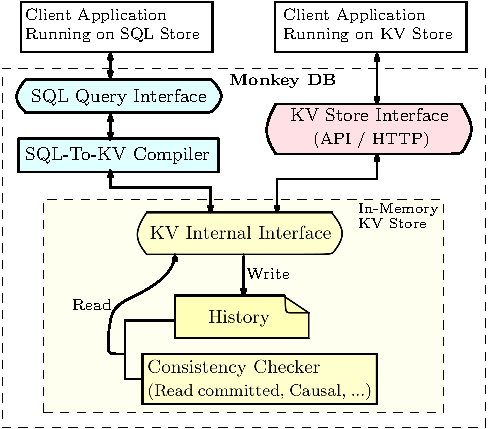
\includegraphics[scale=0.8]{Sources/sql/figures/block_dia.pdf}
\caption{Architecture of \tool{}}
\label{fig:block_dia}
\end{figure}

%The next two sections present an evaluation of \tool{} on a set of
%micro-benchmarks used in prior papers (\sectref{micro}) as well as applications
%from the OLTP benchmark suite \cite{DBLP:journals/pvldb/DifallahPCC13} that consists of
%representative transaction processing workloads running on SQL databases
%(\sectref{oltp}).
%We measure the effectiveness of \tool{} using the \textit{coverage} of weak
%behaviors as well as the ability to break invalid assertions.

%in exploring weak behaviors and in detecting invariant violations on various real-world applications. 
%For this purpose, we used \tool{} in place of actual storage systems and carried out experiments on two sets of benchmarks:
%(1)~a set of microbenchmarks containing shopping cart~\cite{DBLP:conf/pldi/Sivaramakrishnan15}, Twitter~\cite{twissandra}, stack~\cite{DBLP:conf/cav/NagarMJ20} and courseware~\cite{DBLP:conf/esop/NairP020} applications that are representative of real-world services running on Key-Value stores,  
%(2)~a set of applications from OLTP-Bench (Online Transaction Processing) benchmark suite~\cite{DBLP:journals/pvldb/DifallahPCC13} that are representative of transaction processing workloads running on SQL-based relational databases.
%We test these two sets of applications on Key-Value and SQL store interfaces of \tool{} respectively.
%We now discuss our experiments and observed results in detail in Section~\ref{ss:micro} and Section~\ref{sec:oltp}.



  %!TEX root = Thesis.tex

\section{Evaluation: Microbenchmarks}
\label{sec:micro}

We consider a set of micro-benchmarks inspired from real-world applications 
(\sectref{micro-benchmarks}) and evaluate the number of test iterations
required to fail an invalid assertion 
(\sectref{micro-assertion-violations}). We also measure the \textit{coverage} of
weak behaviors provided by MonkeyDB (\sectref{micro-coverage}). Each of these
applications were implemented based on their specifications described in prior
work; they all use MonkeyDB as a library, via its KV interface.  

%, also used in previous work, that are inspired
%from real-world applications:  
%Courseware~\cite{DBLP:conf/esop/NairP020}, Shopping
%cart~\cite{DBLP:conf/pldi/Sivaramakrishnan15} and Twitter~\cite{twissandra}, and
%also a concurrent stack data-structure \cite{DBLP:conf/cav/NagarMJ20}.
%We describe these applications in \sectref{micro-benchmarks}. We
%perform two kinds of experiments. We evaluate the number of test iterations
%required to fail an invalid assertion 
%(\sectref{micro-assertion-violations}) and we also measure the \textit{coverage} of
%weak behaviors provided by MonkeyDB (\sectref{micro-coverage}). Each of these
%use MonkeyDB as a library, via its KV interface.  

\subsection{Applications}
\label{sec:micro-benchmarks}

\paragraph{Twitter \cite{twissandra}}
This is based on a social-networking application that allows users to create a new account, follow,
unfollow, tweet, browse the newsfeed (tweets from users you follow)
and the timeline of any particular user. 
%More formally, $U$ is the set of all users,
%each user has a set of tweets $U.T$, a set of following user $U.FW$ and set of
%followers $U.FR$. 
\figref{twitter-algo} shows the pseudo code for two operations. 
%In \texttt{NewsFeed} and \texttt{Timeline} operations, tweets are
%always returned sorted to the user, by time.

A user can access twitter from multiple clients (sessions), which could lead to
unexpected behavior under weak isolation levels. 
Consider the following scenario with two users, $A$ and $B$ where user $A$ is accessing twitter from two
different sessions, $S_1$ and $S_2$. User $A$ views the timeline of user $B$
from one session (\texttt{$S_1$:Timeline($B$)}) and decides to follow $B$
through another session (\texttt{$S_2$:Follow($A$, $B$)}). Now when user $A$
visits their timeline or newsfeed (\texttt{$S_2$:NewsFeed($A$)}), they expect to
see all the tweets of $B$ that were visible via \texttt{Timeline} in session $S_1$. But
under weak isolation levels, this does not always hold true and there could
be missing tweets. 

\begin{figure}
  \begin{tabular}{@{\hspace{0ex}}l@{\hspace{-1ex}}l}
	\begin{minipage}{4cm}
		\begin{lstlisting}[basicstyle=\ttfamily\footnotesize,escapeinside={(*}{*)},language=MyLang]
			
// Get user's tweets
Timeline(user u) {
  Begin()
  key = "tweets:" + u.id
  T = read(key) 
  Commit()
  return sortByTime(T)
}
		\end{lstlisting}
	\end{minipage}
  &
	%\hspace{-5mm}
	\begin{minipage}{4.3cm}
		\begin{lstlisting}[xleftmargin=3mm,basicstyle=\ttfamily\footnotesize,escapeinside={(*}{*)},language=MyLang]
// Get following users' tweets
NewsFeed(user u) {
  Begin()
  FW = read("following:"+ u.id)
  NF = {}
  foreach v (*$\in$*) FW:
    T = read("tweets:"+ v.id)
    NF = NF (*$\cup$*) T
  Commit()
  return sortByTime(NF)
}
		\end{lstlisting}
	\end{minipage}
\end{tabular}
\vspace{-5ex}
	\caption{Example operations of the Twitter app}
	\label{fig:twitter-algo}
\end{figure}

\vspace{-2mm}
\paragraph{Shopping Cart \cite{DBLP:conf/pldi/Sivaramakrishnan15}}
This application allows a user to add,
remove and change quantity of items from different sessions. It also allows the
user to view all items present in the shopping cart. The pseudo code and
an unexpected behavior under weak isolation levels were discussed in
\sectref{intro}, \figref{motiv}.

\vspace{-2mm}	
\paragraph{Courseware \cite{DBLP:conf/esop/NairP020}}
This is an application for managing students and courses, allowing students
to register, de-register and enroll for courses. Courses can also be created 
or deleted. Courseware maintains the current status of
students (registered, de-registered), courses (active, deleted) as well as
enrollments.
%$S.P$ and $S.N$ are
%the set of registered students and de-registered students respectively.
%Similarly, $C.P$ and $C.N$ are for created and deleted courses. 
Enrollment can contain only registered students and active courses, subject to the capacity
of the course.
%, i.e., $E = \{(u, v) | u \in S.P, v \in C.P\}$ such that $ \forall
%v \in C.P : |\{(u, v) \in E\}| \leq capacity(v)$.  
%\figref{courseware-algo} shows an implementation of the \texttt{Enroll} operation.

Under weak isolation, it is possible that two different students, when trying to
enroll concurrently, will both succeed even though only one spot was left in the
course. Another example that breaks the application is when a student is trying
to register for a course that is being concurrently removed: once the course is
removed, no student should be seen as enrolled in that course.


%\begin{figure}
%\begin{lstlisting}[mathescape=true,language=MyLang]
%Enroll(student s, course c) {
%    Begin()
%    S = read("students") // registered students
%    C = read("courses")  // active courses
%    if (s $\notin$ S || c $\notin$ C)
%      throw InvalidEnrollment;
%    E = read("enrollments")
%    if |{u: (u, c) $\in$ E}| == capacity(c)
%      throw CourseFull;
%    E = E $\cup$ {(s, c)}
%    write("enrollments", E)
%    Commit()
%}
%\end{lstlisting}
%\caption{Courseware implementation of {\tt Enroll}}
%\label{Fi:courseware-algo}
%\end{figure}

\vspace{-2mm}
\paragraph{Treiber Stack \cite{DBLP:conf/cav/NagarMJ20}}
Treiber stack is a concurrent stack data structure that uses 
compare-and-swap (CAS) instructions instead of locks for synchronization. This
algorithm was ported to operate on a kv-store in prior work \cite{DBLP:conf/cav/NagarMJ20}
and we use that implementation. Essentially, the stack contents are placed in
a kv-store, instead of using an in-memory linked data structure.
Each row in the store contains a pair consisting of the stack element and the key of the next
row down in the stack. A designated key ``{\tt head}'' stores the key of the
top of the stack. CAS is implemented as a transaction, but the 
\texttt{pop} and \texttt{push} operations do not use transactions, i.e., each
read/write/CAS is its own transaction.
%The pseudo-code is shown in \figref{stack-algo}. 
%KV stores do not provide a CAS operation, so we implement it at the application level
%using a lock-protected section of a {\tt read} and (if equal) a {\tt write}.
%We determine id of the new node based on
%the current size of the kv-store.


%\begin{figure}
%	\begin{minipage}{4.2cm}
%		\begin{lstlisting}[xleftmargin=4mm,basicstyle=\ttfamily\footnotesize,escapeinside={(*}{*)},language=MyLang]
%Push(v) {
% n = {value: v, next: null};
% while (true) {
%  top = read("head");
%  n.next = top;
%  if (CAS("head", top, n))
%   break;
% }
%}
%		\end{lstlisting}
%	\end{minipage}
%	\begin{minipage}{1mm}
%		||
%	\end{minipage}
%	\hspace{-5mm}
%	\begin{minipage}{4.2cm}
%		\begin{lstlisting}[xleftmargin=5mm,basicstyle=\ttfamily\footnotesize,escapeinside={(*}{*)},language=MyLang]
%Pop() {
% while (true) {
%  top = read("head");
%  if (top == null)
%   return EMPTY;
%  v = top.value;
%  n = top.next;
%  if (CAS("head", top, n))
%   return v;
% }
%}
%		\end{lstlisting}
%	\end{minipage}
%  \caption{Treiber stack implementation. \akash{Might be useful to show the CAS
%  implementation, key generation, etc., but in the appendix.}}
%	\label{Fi:stack-algo}
%\end{figure}

When two different clients try to \texttt{pop} from the stack concurrently, 
under serializability, each \texttt{pop} would return a unique value, assuming that each pushed value is
unique. However, under causal consistency, concurrent \texttt{pop}s can return the same
value.

	

\subsection{Assertion Checking}
\label{sec:micro-assertion-violations}

We ran the above applications with MonkeyDB to find out if assertions, capturing
unexpected behavior, were violated under causal consistency. Table
\ref{tab:assert} summarizes the results. For each application, 
we used 3 client threads and 3 operations per thread. 
We ran each test with MonkeyDB for a total of 10,000 times; we refer to a run as
an iteration. We  report the average number of iterations (Iters) 
before an assertion failed, and the corresponding time taken 
(sec). All the assertions were violated within 58 iterations, in half a second
or less. In contrast, running with an actual database almost never
produces an assertion violation.

\begin{table}[]
	\footnotesize
	\begin{tabular}{|l|l|c|c|}
		
		\hline
		
    \textbf{Application} & \textbf{Assertion}   & \multicolumn{2}{c|}{\textbf{Avg. time to fail}}     \\ 
                         &                      & \textbf{(Iters)} & \textbf{(sec)} \\ \hline
		
    Stack                & Element popped more than once  & 3.7  & 0.02 \\ \hline
		
    Courseware           & Course registration overflow & 10.6 & 0.09  \\ \hline
		
    Courseware           & Removed course registration & 57.5 & 0.52   \\ \hline
		
    Shopping            & Item reappears after deletion & 20.2 & 0.14  \\ \hline
		
    Twitter              & Missing tweets in feed & 6.3 & 0.03 \\ \hline
		
	\end{tabular}
	\caption{\label{tab:assert}Assertions checking results in microbenchmarks}
\end{table}

%\begin{table}[]
%	\footnotesize
%	
%	\begin{tabular}{|c|c|c|c|}
%		
%		\hline
%		
%		\textbf{ID} & \textbf{\# Failed Iters} & \textbf{First Failure} & \textbf{Avg. Time to Fail (s)} \\ \hline
%		
%		A1      &      2673                         &                    9    &     0.02                           \\ \hline
%		
%		A2          & 948                           & 17                     & 0.09                           \\ \hline
%		
%		A3          & 174                           & 18                     & 0.52                           \\ \hline
%		
%		A4          & 496                           & 36                     & 0.14                           \\ \hline
%		
%		A5          &    1595                         &   11                      &  0.03                              \\ \hline
%		
%	\end{tabular}
%	\caption{\label{tab:assert-exp}Assertion failures with MonkeyDB in 10k iterations }
%	
%\end{table}

\subsection{Coverage}
\label{sec:micro-coverage}

The previous section only checked for a particular set of assertions. As an additional measure of
test robustness, we count the number of distinct \textit{client-observable
states} generated by a test. A client-observable state, for an execution, is the vector of values returned by
read operations. For instance, a stack's state is defined by return values of 
\texttt{pop} operations; a shopping cart's state is defined by the return value
of \texttt{GetCart} and so on. 

For this experiment, we randomly generated test harnesses; each harness spawns
multiple threads that each execute a sequence of operations. In order to compute the absolute maximum
of possible states, we had to limit the size of the tests: either 2 or 3
threads, each choosing between 2 to 4 operations. 

Note that any program that concurrently executes operations against a store has
two main sources of non-determinism: the first is the interleaving of operations
(i.e., the order in which operations are submitted to the store) and second is
the choice of read-from (i.e., the value returned by the store under its
configured isolation level). MonkeyDB only controls the latter; it is up to the
application to control the former. There are many tools that systematically enumerate
interleavings (such as \textsc{Chess} \cite{DBLP:conf/pldi/MusuvathiQ08},
\textsc{Coyote} \cite{coyote-web}), but we use a simple trick
instead to avoid imposing any burden on the application: 
we included an option in MonkeyDB to deliberately add a small random
delay (sleep between $0$ to $4$ ms) before each transaction begins. This option 
was sufficient in our experiments, as we show next.

We also implemented a special setup using the \textsc{Coyote} tool \cite{coyote-web} 
to enumerate all sources of non-determinism, interleavings as well as
read-from, in order to explore the entire state space of a
test. We use this to compute the total number of states. \figref{micro_dfs}
shows the number of distinct 
states observed under different isolation levels, averaged across multiple ($50$) test
harnesses. For each of serializability and causal consistency, we show the max
(as computed by \textsc{Coyote}) and versions with and without the delay option
in MonkeyDB. 

Each of these graphs show similar trends: the number of states with
causal consistency are much higher than with serializability. Thus, testing with a
store that is unable to generate weak behaviors will likely be ineffective.
Furthermore, the ``delay'' versions of MonkeyDB are able to approach the 
maximum within a few thousand attempts, implying that MonkeyDB's strategy of
per-read randomness is effective for providing coverage to the application.


\begin{figure*}[h]
	
	\centering
	
	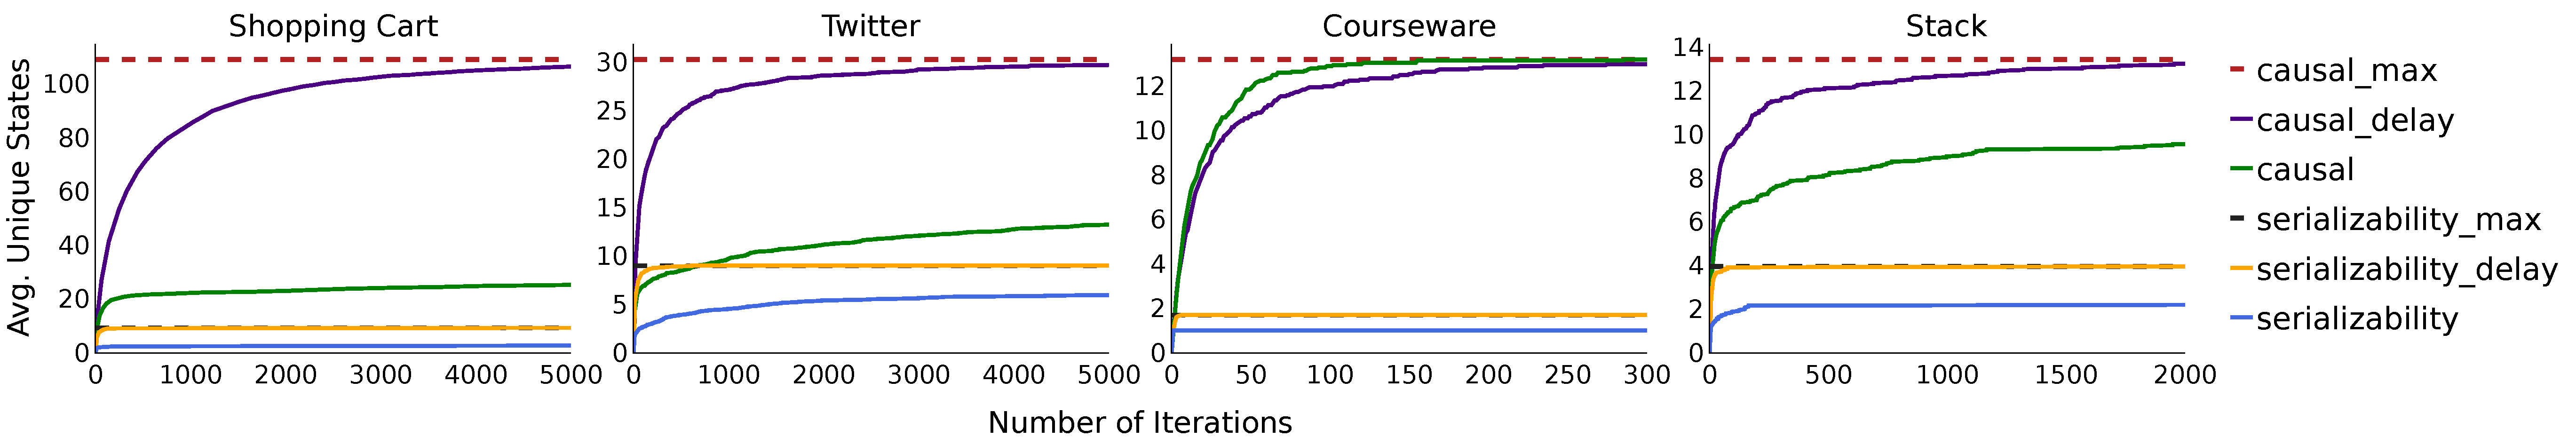
\includegraphics[width=1.0\textwidth]{Sources/sql/plots/random_avg.pdf}
	
	\caption{State coverage obtained with MonkeyDB for various microbenchmarks}
	
	\label{fig:micro_dfs}
\end{figure*}

%\begin{figure}[h]
%
%	\centering
%
%	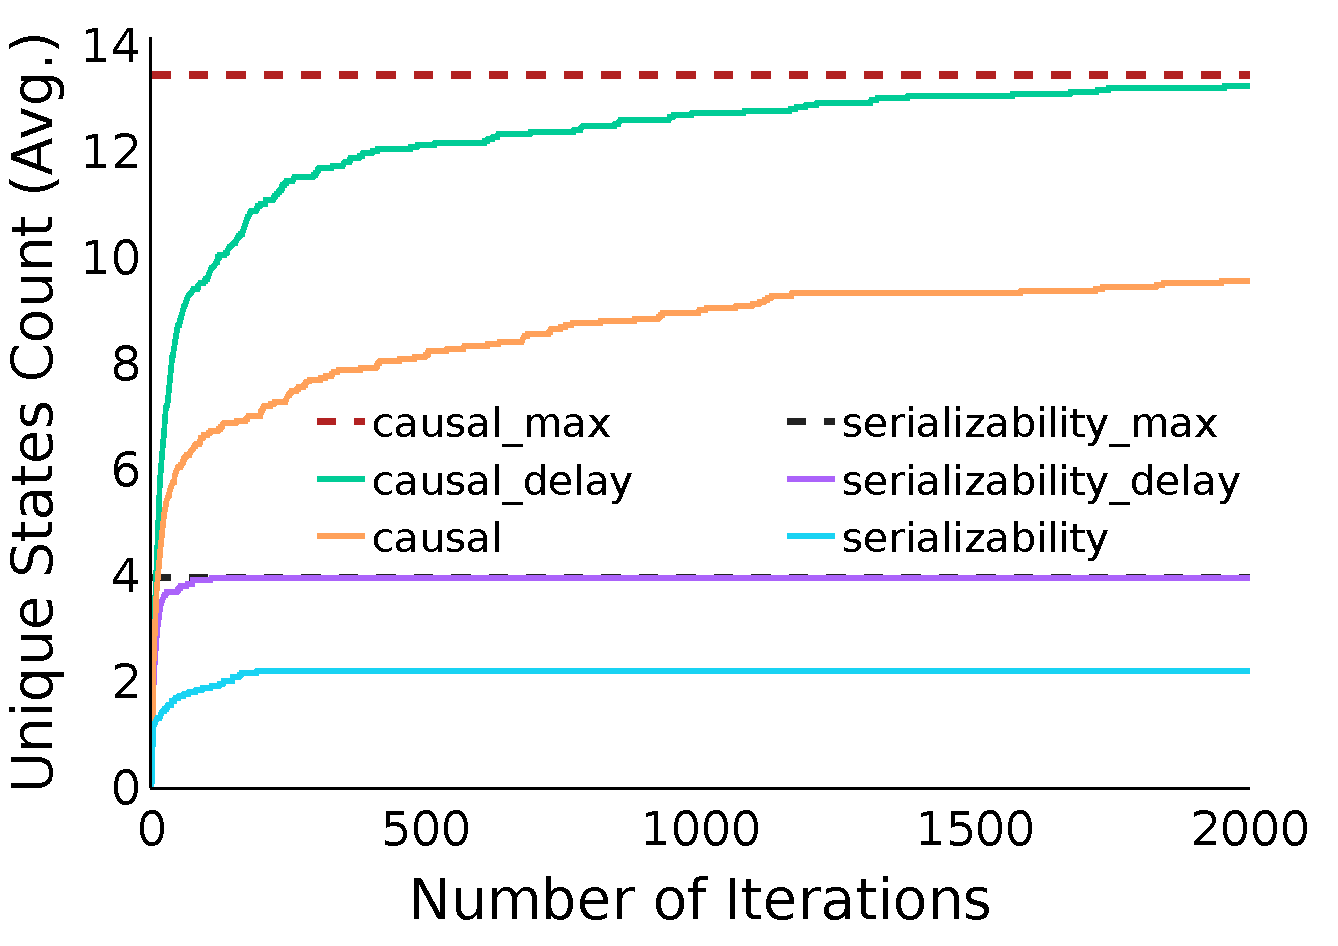
\includegraphics[width=0.4\textwidth]{plots/stack_random_avg.pdf}
%
%	\caption{Stack complete state exploration}
%
%	\label{fig:stack_dfs}
%\end{figure}
%
%
%\begin{figure}[h]
%	
%	\centering
%	
%	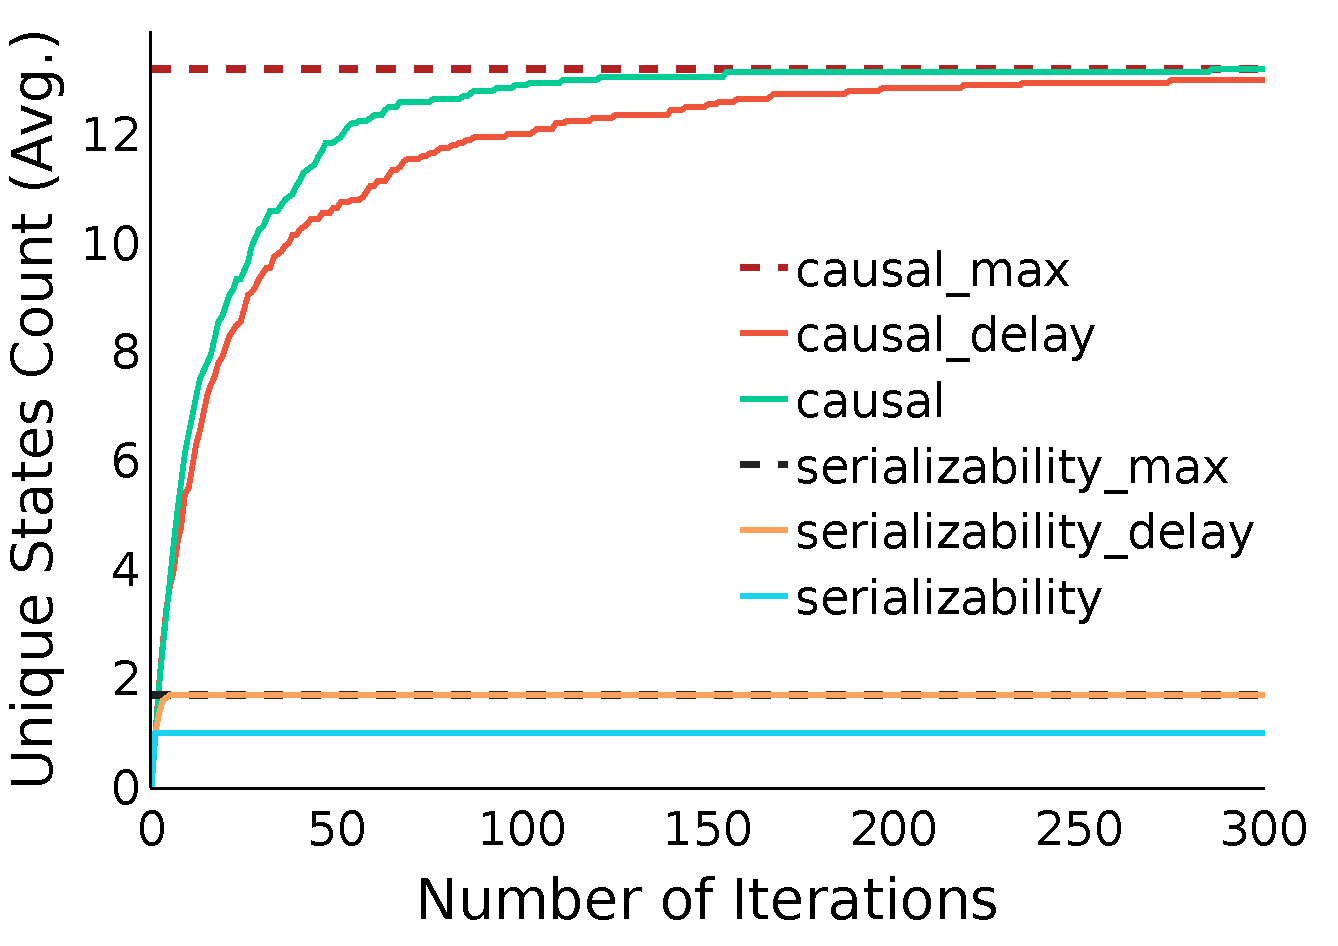
\includegraphics[width=0.4\textwidth]{plots/courseware_random_avg.pdf}
%	
%	\caption{Courseware complete state exploration}
%	
%	\label{fig:course_dfs}
%\end{figure}
%
%
%\begin{figure}[h]
%	
%	\centering
%	
%	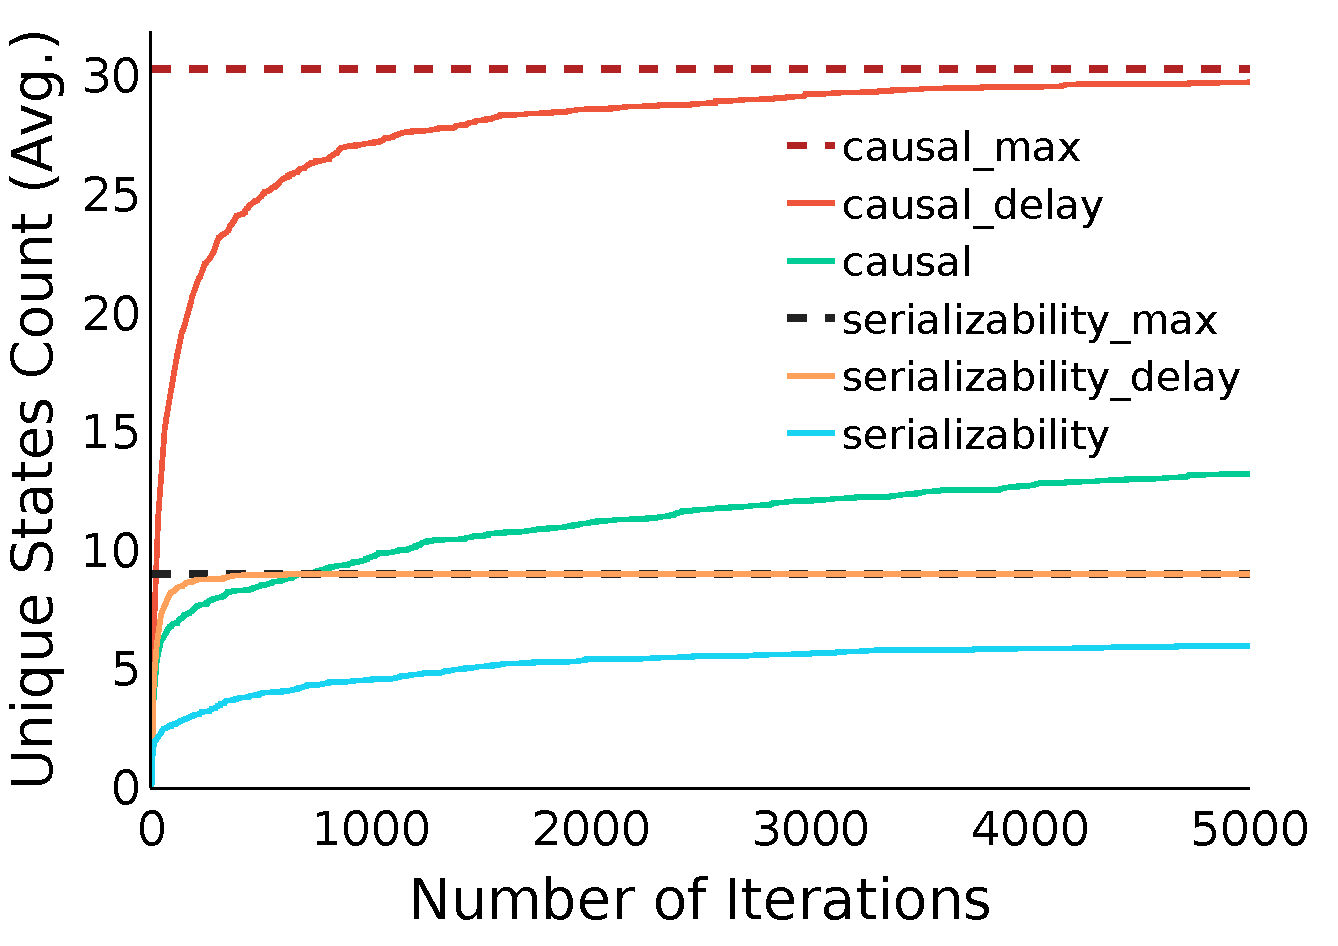
\includegraphics[width=0.4\textwidth]{plots/shopping_cart_random_avg.pdf}
%	
%	\caption{Shopping cart complete state exploration}
%	
%	\label{fig:cart_dfs}
%\end{figure}
%
%\begin{figure}[h]
%	
%	\centering
%	
%	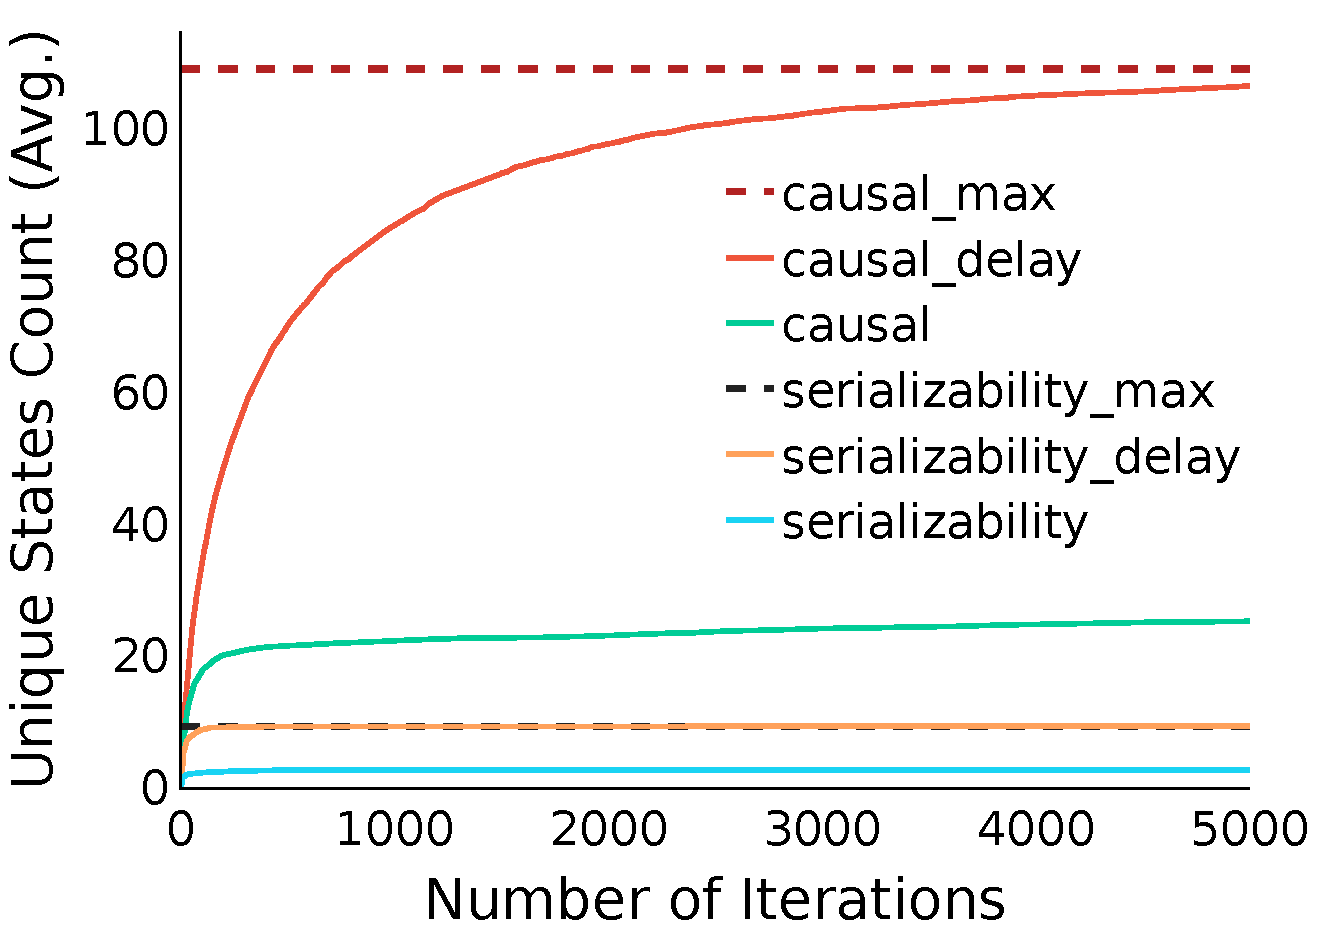
\includegraphics[width=0.4\textwidth]{plots/twitter_random_avg.pdf}
%	
%	\caption{Twitter complete state exploration}
%	
%	\label{fig:twitter_dfs}
%\end{figure}


%In the previous experiment, we were limited by DFS to explore all possible
%states, as it takes time to finish even for smaller test cases. We now show the
%effect of increasing the size of test case on the number of unique states
%observed. Figure \ref{fig:states_ops} shows the plot for stack application. We
%run stack application for 10,000 iterations with 3 threads and vary the number
%of operations per thread from 2 to 5. The states increase exponentially in
%causal consistency, but as we go towards larger test case, states tend to reach
%the upper limit possible to explore within 10,000 iterations.

%\begin{figure}[h]
%	
%	\centering
%	
%	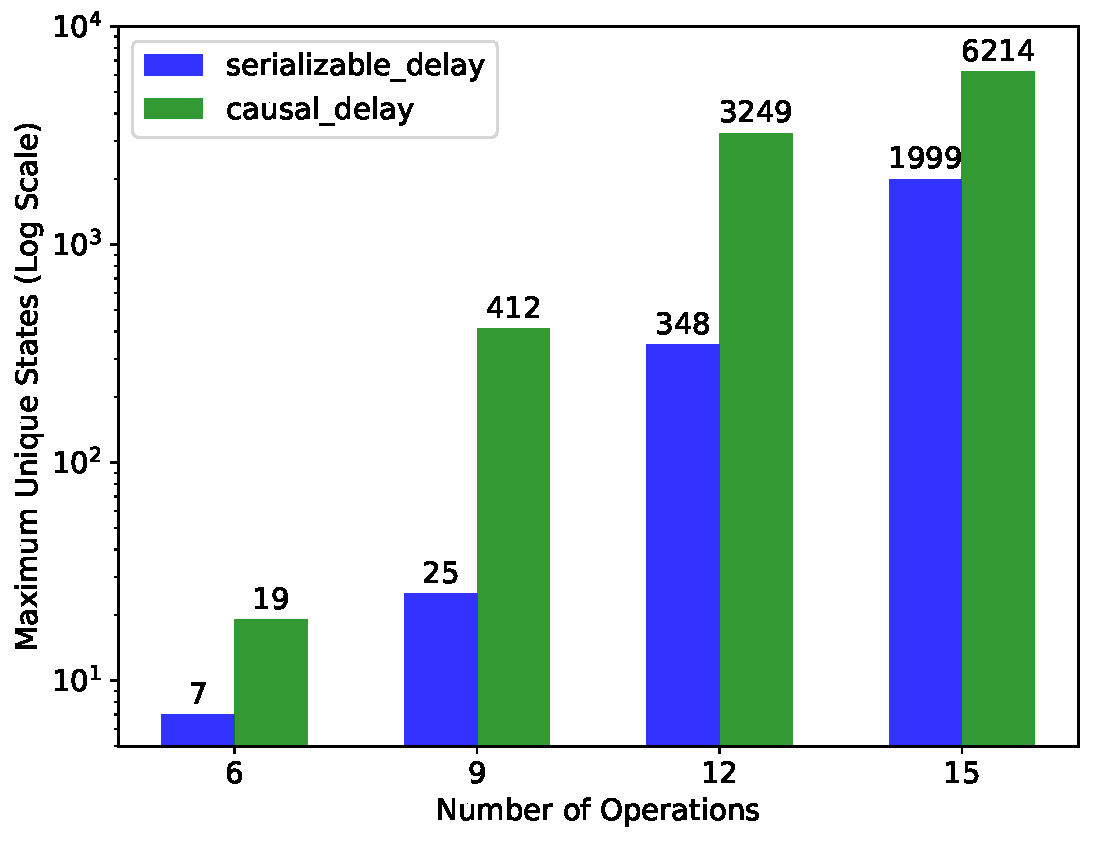
\includegraphics[width=0.5\textwidth]{plots/stack_states_op.pdf}
%	
%	\caption{Stack - maximum states possible with different operations}
%	
%	\label{fig:states_ops}
%\end{figure}

  %!TEX root = Thesis.tex

\section{Evaluation: OLTP Workloads}
\label{sec:oltp}

OLTPBench \cite{DBLP:journals/pvldb/DifallahPCC13} is a benchmark suite of representative 
OLTP workloads for relational databases.
%, obtained from applications such as
%wholesale supply, banking, seat booking, voting, collaborative-editing and so on. 
%OLTPBench consists of a configurable 
%load generator that takes care of populating database tables, followed by
%issuing various different transactions in a desired proportion. 
We picked a subset of OLTPBench for which we had reasonable assertions. 
Table~\ref{table-bench} lists basic
information such as the number of database tables, the
number of static transactions, how many of them are read-only, and the number of
different assertions corresponding to system invariants for testing the benchmark. 
%We included TPC-C, the
%most widely known benchmark, and a few others for which we could come up with
%reasonable assertions. 
We modified OLTPBench by rewriting SQL join and aggregation
operators 
%(16.67\% of total queries) 
into equivalent application-level
loops, following a similar strategy as prior work \cite{DBLP:journals/pacmpl/RahmaniNDJ19}. Except for
this change, we ran OLTPBench unmodified. 

For TPC-C, we obtained a set of $12$ invariants from its specification
document~\cite{tpcc-spec}. For all other benchmarks, we manually identified 
invariants that the application should satisfy. We asserted these invariants 
by issuing a read-only transaction to \tool{} 
at the end of the execution of the benchmark. 
None of the assertions fail under serializability; they are indeed invariants
under serializability.\footnote{We initially observed two assertions failing
under serializability. Upon analyzing the code, we identified that the
behavior is due to a bug in OLTPBench that we have reported to the authors (link
ommitted).} 
%We use \tool{} to test their
%validity under causal consistency and read committed isolation levels. 
When using weaker isolation, we configured MonkeyDB to use latest reads only
(\sectref{impl}) for the assertion-checking transactions 
in order to isolate the weak behavior to only the application. 

We ran each benchmark $100$ times and report, for each assertion, the number of
runs in which it was violated. Note that OLTPBench runs in two phases. The first
is a loading phase that consists of a big initial transaction to populates tables 
with data, and then the execution phase issues multiple concurrent transactions. 
With the goal of testing correctness, we \textit{turn down} the scale factor to
generate a small load and limit the execution phase time to ten seconds with 
just two or three sessions. A smaller test setup has the advantage
of making debugging easier. With \tool{}, there is no need to generate large
workloads.

%We first discuss our results on TPC-C~\cite{tpcc-bench} in detail followed by
%other benchmarks,
% as TPC-C specifies its invariants and all its invariants are well studied by
% previous works~\cite{DBLP:journals/pacmpl/RahmaniNDJ19,DBLP:journals/pvldb/GanRRB020}.
%We first discuss our results on SmallBank, SEATS, Voter and Wikipedia, followed by TPC-C in detail.

\begin{table}
  \footnotesize
	\begin{tabular}{|l|c|c|c|c|}
    \hline
		Benchmark & \#Tables & \#Txns &\#Read-only & \#Assertions \\ \hline
		TPC-C &  9 & 5 & 2& 12\\
		SmallBank & 3 & 6 & 1 & 1\\
		Voter & 3 & 1 & 0 & 1\\
		Wikipedia & 12 & 5 & 2 & 3\\
		\hline
	\end{tabular}	
	\caption{OLTP benchmarks tested with \tool{}}
	\label{table-bench}
\end{table}


\paragraph{TPC-C} TPC-C emulates a wholesale supplier transactional system
that delivers orders for a warehouse company.
This benchmark deals with customers, payments, orders, warehouses, 
deliveries, etc. 
%As listed in Table~\ref{table-bench}, it has five transactional procedures, out
%of which three (new order, payment and delivery) modify the database and two
%(order status and stock level) are read-only.
We configured OLTPBench to issue a higher proportion ($>85\%$) of update
transactions, compared to read-only ones.  
%(29, 29, 8, 29, 5)
Further, we considered a small input workload constituting of one warehouse, two
districts per warehouse and three customers per district.

%TODO A12 IS THE ASSERTION WHERE WE REPLACED EQUALITY WITH >= ?
%Ans: NO. THAT IS A11

TPC-C has twelve assertions (A1 to A12) that check for consistency between 
the database tables.
For example, A12 checks: for any customer, the sum of delivered order-line
amounts must be equal to the sum of balance amount and YTD (Year-To-Date)
payment amount of that customer.
%C_BALANCE + C_YTD_PAYMENT = sum(OL_AMOUNT)
%We observed that all these assertions succeed under Serializability, 
%when tested both on \tool{} and on a real database
%MariaDB~\cite{mariadb}\footnote{We initially observed two assertions failing
%under Serializability. Upon analyzing the code, we identified that the
%behavior is due to a bug in OLTPBench that we have reported to the authors (link
%ommitted).}. 
%(\url{https://github.com/oltpbenchmark/oltpbench/issues/345}).}.
%We ran TPC-C for 100 times.
%To test whether they preserve under weak behaviors, we run the benchmark on
%\tool{} under Causal and Read Committed isolation levels, for 100 test
%iterations.

\begin{figure*}[!ht]
    \centering
    \begin{minipage}{0.47\textwidth}
        \centering
    	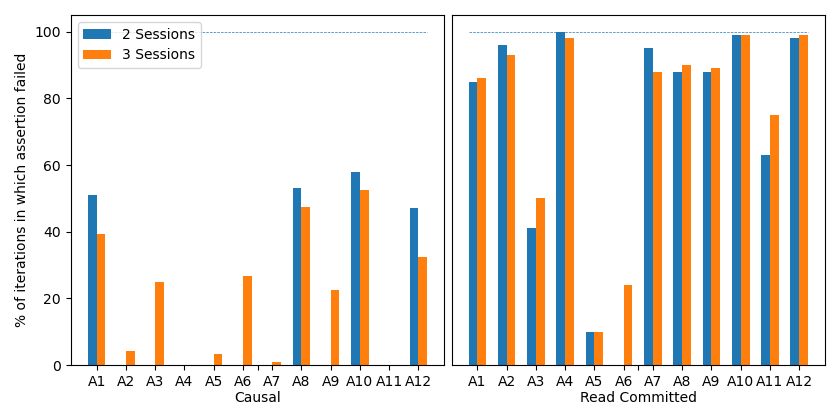
\includegraphics[scale=0.4]{Sources/sql/plots/random_strongest_tpcc.png}
	    \caption{\small Assertion checking: {TPC-C}}
        \label{fig:tpcc}
    \end{minipage}\hfill
    \begin{minipage}{0.47\textwidth}
        \centering
    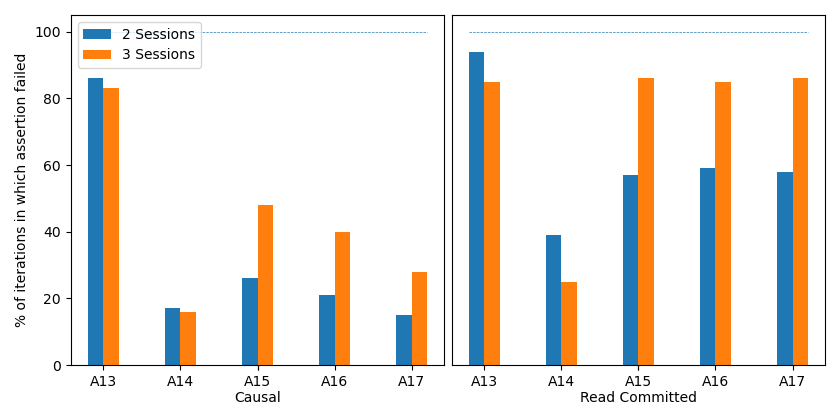
\includegraphics[scale=0.4]{Sources/sql/plots/random_strongest_all.png}
	    \caption{\small Assertion checking: SmallBank, Voter, and Wikipedia}
    \label{fig:rest}
    \end{minipage}
\end{figure*}

Figure~\ref{fig:tpcc} %and Figure~\ref{fig:tpcc-rc} 
shows the percentage of test runs in which an assertion failed. 
%Figure~\ref{fig:tpcc-rc} 
It shows that all the twelve assertions are violated under
Read~Committed isolation level. In fact, $9$ out of the $12$ 
assertions are violated in more than 60\% of the test runs.
In case of causal, %(Figure~\ref{fig:tpcc}), 
all assertions are violated
with three sessions, except for A4 and A11. We manually inspected TPC-C and
we believe that both these assertions are valid under causal consistency. 
For instance, A4 checks for consistency between two tables, both of which are
only updated within the same transaction, thus causal consistency is enough to
preserve consistency between them.
%For instance, A04 checks that for each district, the number of order lines of all 
%the orders in that district (obtained from ORDER\_LINE table) is the same as 
%the sum of order-line counts maintained for the corresponding orders (in the ORDER
%table). Both the concerned tables (ORDER\_LINE and ORDER) are updated within the same transaction,
%thus causal consistency is enough to ensure that they remain consistent with each
%other. 

%These results demonstrate the effectiveness of \tool{} in breaking (invalid) 
%assertions.

%To understand why A04 and A11 did not violate under Causal, we analyzed the two
%assertions and the transactional procedures associated with them in TPC-C.
%In our analysis, we found that it is not possible to violate A04 and A11 under
%Causal or any other stronger isolation levels.
%For example, A04 checks for every district, the number of order lines of all 
%the orders in that district (obtained from ORDER\_LINE table) is same as 
%the sum of order-line counts maintained for the corresponding orders (in ORDER
%table).
%This assertion cannot be violated under Causal because the insertions to both
%tables happen atomically in a single transactional procedure (`new
%order').
%A04: For every district, the number of orderlines of all orders is same as sum of orderline count (number of orderlines). %defined in order table.  
%sum(O_OL_CNT) = [number of rows in the ORDER-LINE table for this district]
%A11: For every district and every customer, the difference between number of orders and number of new orders must be equal to 2100.
%(count(*) from ORDER) - (count(*) from NEW-ORDER) = 2100

%\akash{This para can be skipped.}
%We also observed that MonkeyDB's read selection strategy had minor impact on the
%results. Choosing weakest-read gave geo-mean disimprovement of 27.1\%,
%whereas weak-biased-read gave geo-mean disimprovement of 61.7\%.   
%Similarly, instead of strongest-read strategy for the assertion checks, we
%used the same read strategy as the one used for the test. In this case, 
%random-read gave a geo-mean disimprovement of 36.2\%, weakest-read gave 
%geo-mean disimprovement of 53.9\%, weak-biased-read gave a geo-mean
%disimprovement of 73.7\%.
%These numbers indicate that the default random-read and strongest-read strategy
%combination works well in practice.

These results demonstrate the effectiveness of \tool{} in breaking (invalid) 
assertions. Running with MySQL, under read committed, was unable to violate any assertion except for
two (A10 and A12), even when increasing the number of sessions to $10$. We used
the same time limit of $10$ seconds for the execution phase. We note that MySQL
is much faster than MonkeyDB and ends up processing up to $50\times$ more
transactions in the same time limit, yet is unable to violate most assertions. 
Prior work \cite{DBLP:journals/pacmpl/RahmaniNDJ19} attempted a more sophisticated test
setup where TPC-C was executed on a Cassandra cluster, while running 
Jepsen~\cite{jepsen} for fault injection. This setup also was unable to violate 
all assertions, even when running without transactions, and on a weaker isolation level than read committed. 
Only six assertions were violated with 10 sessions, 
eight assertions with 50 sessions, and ten assertions with 100 sessions.
With \tool{}, there is no need to set up a cluster, use fault injection or
generate large workloads that can make debugging very difficult. 


%\begin{figure}
%    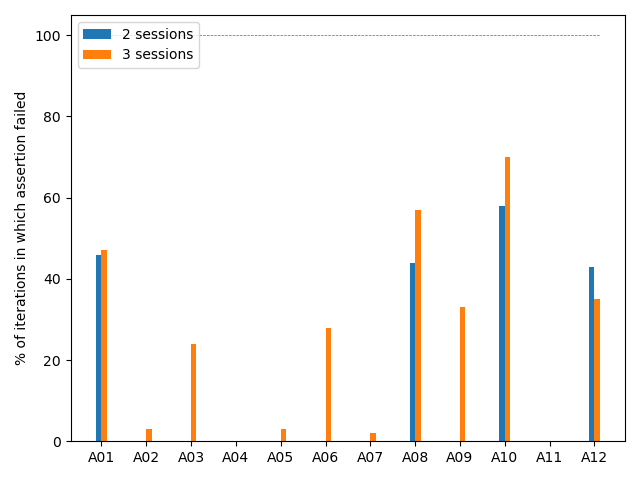
\includegraphics[scale=0.4,width=0.48\textwidth]{plots/tpcc_causal.png}
%    \caption{Assertion Violations under Causal Consistency.}
%    \label{fig:tpcc-causal}
%\end{figure}
%\begin{figure}
%    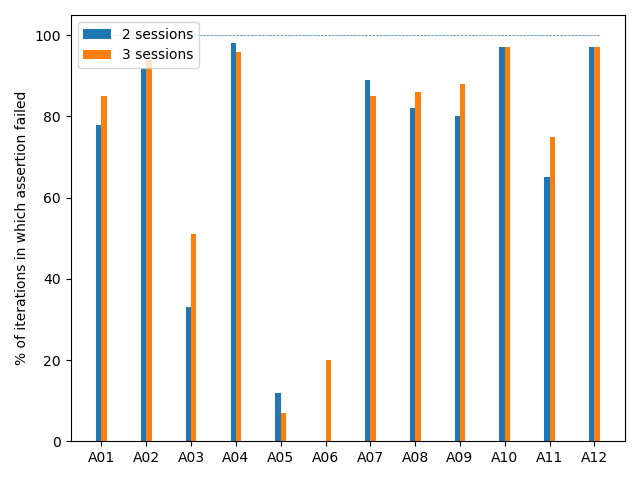
\includegraphics[scale=0.4,width=0.48\textwidth]{plots/tpcc_readcommitted.png}
%    \caption{Assertion Violations under Read Committed.}
%    \label{fig:tpcc-rc}
%\end{figure}
%

\paragraph{SmallBank, Voter, and Wikipedia} 
SmallBank is a standard financial banking system, dealing with customers, saving
and checking accounts, money transfers, etc.  
Voter emulates the voting system of a television show and allows users to vote for their favorite contestants.
%Concurrent votes by a user to the same contestant brings in complexity to the voting system. 
Wikipedia is based on the popular online encyclopedia. It deals with a complex database schema involving 
page revisions, page views, user accounts, logging, etc.  
It allows users to edit its pages and maintains a history of page edits and user actions. 
%Data contention in this system arises when multiple users edit the same page or when the same user edits a page from multiple sessions.

We identified a set of five assertions, A13 to A17, that should be satisfied by these systems.  
%Among the five assertions, three are from Wikipedia, and one each from SmallBank and Voter systems.
For SmallBank, we check if the total money in the bank remains the same while it
is transfered from one account to another (A13). 
Voter requires that the number of votes by a user is limited to a fixed threshold (A14).  
For Wikipedia, we check if for a given user and for a given page, the number of
edits recorded in the user information, history, and logging tables
%(USERACCT, RECENTCHANGES, and LOGGING tables) 
are consistent (A15-A17). 
%All these assertions are preserved under Serializability isolation level.
%We test these systems on \tool{} for assertion violations under Causal and Read Committed isolation levels.
%For all these benchmarks, we configure the weights of transactional procedures in OLTP-Bench 
%such that the transactions which update are executed more often.   
As before, we consider small work loads: (1) five customers for SmallBank, (2) one user for Voter, and (3) two pages and two users for Wikipedia.  

Figure~\ref{fig:rest} shows the results. 
\tool{} detected that all the assertions are invalid under the chosen isolation levels.
Under causal, \tool{} could break an assertion in 26.7\% (geo-mean) runs given 2 sessions and in 37.2\% (geo-mean) runs given 3 sessions.
Under read committed, the corresponding numbers are 56.1\% and 65.4\% for 2 and
3 sessions, respectively.
%Our results in this experiment confirm the generality and effectiveness of \tool{} in detecting assertion violations in diverse OLTP environments. 

%\begin{figure}[t]
%    \includegraphics[scale=0.4,width=0.48\textwidth]{plots/all_random_strongest.png}
%    \caption{\small Assertions violated under Causal and Read~Committed}
%    \label{fig:diverse-bench}
%\end{figure}

  %!TEX root = Thesis.tex

\section{Testing SQL Database}
\label{sec:app:related}

%AXIOMATIC FORMALIZATIONS OF ISOLATION LEVELS (ADYA, GOTSMAN, OOPSLA). RELATED TO WEAK CONSISTENCY FOR INDIVIDUAL OPERATIONS (POPL'14, ETC)

There have been several directions of work addressing the correctness of database-backed applications. 
We directly build upon one line of work concerned with the logical formalization
of isolation levels 
\cite{ansi,DBLP:conf/icde/AdyaLO00,DBLP:conf/sigmod/BerensonBGMOO95,DBLP:conf/concur/Cerone0G15,DBLP:journals/pacmpl/BiswasE19}.
Our work relies on the axiomatic definitions of isolation levels, as given
in~\cite{DBLP:journals/pacmpl/BiswasE19}, which also investigated
the problem of checking whether a given history satisfies a certain isolation
level. Our kv-store implementation relies on these algorithms 
to check the validity of the values returned by read operations. Working with a
logical formalization allowed us to avoid implementing an actual database with replication or
sophisticated synchronization.

Another line of work concentrates on the problem of finding ``anomalies'': 
behaviors that are not possible under serializability. This is typically done
via a static analysis of the application code that builds a static dependency graph that
over-approximates the data dependencies in all possible
executions of the application~\cite{DBLP:journals/jacm/CeroneG18,DBLP:journals/jacm/CeroneG18,DBLP:conf/concur/0002G16,DBLP:journals/tods/FeketeLOOS05,DBLP:conf/vldb/JorwekarFRS07,DBLP:conf/sigmod/WarszawskiB17,DBLP:journals/pvldb/GanRRB020}.
Anomalies with respect to a given isolation level then corresponds to a
particular class of cycles in this graph. Static dependency graphs turn out to
be highly imprecise in representing feasible executions, leading to false
positives. Another source of false positives is that an anomaly might not be a
bug because the application may already be designed to handle the
non-serializable behavior \cite{DBLP:conf/pldi/BrutschyD0V18,DBLP:journals/pvldb/GanRRB020}. 
Recent work has tried to address these issues by using more precise 
logical encodings of the application,
e.g.~\cite{DBLP:conf/popl/BrutschyD0V17,DBLP:conf/pldi/BrutschyD0V18} or
by using user-guided heuristics~\cite{DBLP:journals/pvldb/GanRRB020}. 

Another approach consists of modeling the application
logic and the isolation level in first-order logic and relying on SMT solvers to
search for anomalies~\cite{DBLP:journals/pacmpl/KakiESJ18,DBLP:conf/concur/NagarJ18,burcu-netys},
or defining specialized reductions to assertion
checking~\cite{DBLP:conf/concur/BeillahiBE19,DBLP:conf/cav/BeillahiBE19}.
The \textsc{Clotho} tool \cite{DBLP:journals/pacmpl/RahmaniNDJ19}, for instance, uses a static analysis of the application to
generate test cases with plausible anomalies, which are deployed in a concrete
testing environment for generating actual executions. 

Our approach, based on testing with MonkeyDB, has several practical advantages.
There is no need for analyzing application code; we can work with any
application. There are no false positives because we directly run the
application and check for user-defined assertions, instead of looking for
application-agnostic anomalies. The limitation, of course, is
the inherent incompleteness of testing.

Several works have looked at the problem of reasoning about the correctness of
applications executing under weak isolation and introducing additional
synchronization when
necessary~\cite{DBLP:conf/eurosys/BalegasDFRPNS15,DBLP:conf/popl/GotsmanYFNS16,DBLP:conf/esop/NairP020,DBLP:conf/usenix/0001LCPRV14}.
As in the previous case, our work based on testing has the advantage that it can
scale to real sized applications (as opposed to these techniques which are based
on static analysis or logical proof arguments), but it cannot prove that an
application is correct. Moreover, the issue of repairing applications is
orthogonal to our work. 
% works rely on static analysis or logical proof arguments whose application to  is limited. 

From a technical perspective, our operational semantics based on recording past
operations and certain data-flow and control-flow dependencies is similar to
recent work on stateless model checking in the context of weak memory
models,
e.g.~\cite{DBLP:journals/pacmpl/Kokologiannakis18,DBLP:conf/tacas/AbdullaAAJLS15}.
This work, however, does not consider transactions. Furthermore, their focus is on
avoiding enumerating equivalent executions, which is beyond the scope of our
work (but an interesting direction for future work).

%Proof techniques [CISE, Petri, Alvaro..]. Apply to particular isolation levels and to toy examples, hard to scale.
%
%Dynamic analyses [Acid, IsoDiff]: imprecise, or user input required

%TECHNICALLY, THE OPERATIONAL SEMANTICS BASED ON MAINTAINING A HISTORY IS RELATED TO OTHER WORKS IN WEAK MEMORY (VAFEAIDIS, PAROSH)



%To address developers' concerns in reasoning weak behaviours and in detecting invariant violations, 
%there were recent efforts spanning static analyses~\cite{DBLP:journals/pacmpl/RahmaniNDJ19, burcu-netys}, dynamic analyses~\cite{DBLP:conf/sigmod/WarszawskiB17, DBLP:journals/sigsoft/DabaghchianROMT17}, and testing~\cite{jepsen}.
%
%Static analyses~\cite{DBLP:journals/pacmpl/RahmaniNDJ19,burcu-netys} encode transactions, database consistency specification, and application invariant (sometimes) etc., in verification logic and use SMT solvers to prove that logical formula.
%While these static analyses provide full guarantees, using them requires expertise and also handling arbitrary code becomes challenging.
%\tool{} requires no modifications to the client appication under test.
%Also, new changes to the application may require renewed analysis, and using \tool{},
%developers must be able to perform testing as a continual activity as the application evolves.
%
%
%Dynamic analyses~\cite{DBLP:conf/sigmod/WarszawskiB17,DBLP:journals/sigsoft/DabaghchianROMT17} work on the abstract models built from the actual execution trace.
% These techniques require instrumenting the application code and it becomes difficult to replay the findings of such an analysis in the actual test environment because the analysis was performed offline (not during execution), and also  the offline analysis can sometimes suffer from false positives.   
%
%
%Although there are no automatic testing tools dedicated to database applications, random fuzzing based testing tools such as Jepsen~\cite{jepsen} designed for distributed applications can be used. 
%However, these tools cannot provide high coverage.

  %!TEX root = Thesis.tex

\section{SQL database}
\label{sec:conc}

Our goal is to enable developers to test the correctness of their storage-backed applications under 
weak isolation levels. Such bugs are hard to catch because weak behaviors are
rarely generated by real storage systems, but failure to address them can lead
to loss of business \cite{acidrain}. We present MonkeyDB, an easy-to-use mock storage system
for weeding out such bugs. MonkeyDB uses a logical understanding of isolation
levels to provide (randomized) coverage of all possible weak behaviors. Our evaluation reveals that
using MonkeyDB is very effective at breaking assertions that would otherwise
hold under a strong isolation level.



  \chapter{Conclusion}
  %!TEX root = ../Thesis.tex

This dissertation introduces some previously unexplored open problems in the distributed domains. In general, many of the weak consistencies and data types are not formally characterized. The state of the art testing frameworks are still using ad-hoc setup and network manipulation without giving proper testing coverage. We provide formal characterizations for these systems and come up with algorithms which are able to provide sound and complete testing and provide better coverage.

\section{Conflict-Free Replicated Data types}

At first, we provide formal characterizations for conflict free replicated data types. The characterizations enable us to reason about the admissibility of the histories of these data types corresponding to their weaker consistencies. We further explore the asymptotic complexities of the checking admissibility of these histories. We prove intractability and tractability results for these data types.

\subsection{Future Work}

The general problem of checking admissible problems for Flags, Set still remains open. We provide a sound algorithm which runs in polynomial-time.


\section{Transactional Systems}

Then, we move on to transactional systems with reads and writes. We explore different levels of weak consistencies for transactional systems. We propose novel characterizations for these weak consistencies over transactional systems. Using these characterizations we study the asymptotic complexities of checking these consistencies for transactional histories. We prove intractability and tractability results for these weak consistencies. But at the end, we show these intractable cases are tractable if we bound the number of sessions in the histories. We further extend this idea on a graph replicas where the bi-connected components are bounded.

\subsection{Future Work}

We provide a complete framework to test transactional systems. The possible next work would be find root causes for inconsistent history. Sometimes, the bugs are not visible in small number of sessions. Our tests on AntidoteDB exposed a bug when the number of sessions is 42. When the number of history is too big, it is natural to ask the smallest sub-history which violates the consistency. Although it is straightforward to see how one would give a solution to this problem, but for a efficient and online algorithm we keep this problem for future.

Next we can try to extend our algorithm to an online one. For now, we run the algorithm offline \ie we run the system and log the history at first, then run our algorithm. This is enough for unit tests, but in production, someone would want to run an auditor like tool to make sure the consistency of these systems are maintained all the time. Also, when an inconsistency is detected how to detect the root cause of the inconsistency bug and recover from it. 

\section{Applications Using Transactional Systems}

Having these two previous results, we explore if we can use our characterizations to test distributed applications built on top of some distributed systems. Usually these tests are done on real databases relying on artificial network manipulation. Since these systems are optimized for corner cases, it is very very hard to find the bugs due to corner cases. So these unit tests do not give good coverage. We presented \tool{}, which models different weak consistency levels using our characterizations. \tool{} simulates a consistency keeping track of a global history and making uniform choices which satisfies the characterization axioms. This drastically improves the test coverage, and we imperically show \tool{} were very quick to violate invariants in popular OLTP benchmarks.

\subsection{Future Work}

One of the problem that developers come across often is to write good sets of invariants for unit tests. We provide a formal characterizations for weak consistencies.

It would be interesting to see, provided a distributed application and the consistency level required, can we generate sets of invariants for that applications which robustly captures the bugs when run on some weaker consistency levels.

It would also be an interesting problem to find the weakest possible consistency level where the application still runs correctly. This would help the developers to choose the best consistency levels for their application, yet increase the concurrency of their application communication.

In modern databases, sometimes the operations are performed different level of consistency levels. It would be interesting to study the characterization problem of these hybrid-consistency problem and provide tractable admissiblity checking algorithms.

\tool{} is a prototype of our idea. Although it is made to work on OLTPBenchmark, the current versions of real world applications require far more engineering to make it work with \tool{}. We want to finish that work to provide a complete standalone mock database which can be used to test a larger set of real world applications. 

% This ensures that the subsequent sections are being included as root
% items in the bookmark structure of your PDF reader.
\bookmarksetup{startatroot}
\backmatter

  % \begingroup
  %   \let\clearpage\relax
  %   \glsaddall
  %   \printglossary[type=\acronymtype]
  %   \newpage
  %   \printglossary
  % \endgroup

  \printindex
  \printbibliography

\end{document}
